% This is an AMS-LaTeX v. 1.2 File.

\documentclass[leqno]{report}
%\usepackage{amsmath}
\usepackage{amsthm}
\usepackage{amssymb}
%\usepackage{amsfonts}
\usepackage{amsxtra}     % Use various AMS packages
\usepackage{rac}         % Use Rackham thesis macros
\usepackage{dbl12}
%\usepackage{srcltx}
\usepackage{epsfig}
\usepackage{verbatim}
\usepackage{hyperref}
\usepackage{xcolor}
\usepackage{multirow}
\usepackage{rotating}

\hypersetup{
    colorlinks = false,
    linkbordercolor = {white},
    citebordercolor = {white}
}
%%%%%%%%%%%%%%%%%%%%%%%%%%%%%%%%%%%%%%%%%%%%%%%%%%%%%%%%%%%%%%%%%%%%%%%%%%%%%%

% Redefine margins and other page formatting

\setlength{\oddsidemargin}{0.5in}

%%%%%%%%%%%%%%%%%%%%%%%%%%%%%%%%%%%%%%%%%%%%%%%%%%%%%%%%%%%%%%%%%%%%%%%%%%%%%%%

% Various theorem environments. All of the following have the same numbering
% system as theorem.

\theoremstyle{plain}
\newtheorem{theorem}{Theorem}
\newtheorem{prop}[theorem]{Proposition}
\newtheorem{corollary}[theorem]{Corollary}
\newtheorem{lemma}[theorem]{Lemma}
\newtheorem{question}[theorem]{Question}
\newtheorem{conjecture}[theorem]{Conjecture}
\newtheorem{assumption}[theorem]{Assumption}

\theoremstyle{definition}
\newtheorem{definition}[theorem]{Definition}
\newtheorem{notation}[theorem]{Notation}
\newtheorem{condition}[theorem]{Condition}
\newtheorem{example}[theorem]{Example}
\newtheorem{introduction}[theorem]{Introduction}

\theoremstyle{remark}
\newtheorem{remark}[theorem]{Remark}
\include{header}
%%%%%%%%%%%%%%%%%%%%%%%%%%%%%%%%%%%%%%%%%%%%%%%%%%%%%%%%%%%%%%%%%%%%%%%%%%%%%%%

\numberwithin{theorem}{chapter}        % Numbers theorems "x.y" where x
                                        % is the section number, y is the
                                        % theorem number

%\renewcommand{\thetheorem}{\arabic{chapter}.\arabic{theorem}}

%\makeatletter                          % This sequence of commands will
%\let\c@equation\c@theorem              % incorporate equation numbering
%\makeatother                           % into the theorem numbering scheme

%\renewcommand{\theenumi}{(\roman{enumi})}

%%%%%%%%%%%%%%%%%%%%%%%%%%%%%%%%%%%%%%%%%%%%%%%%%%%%%%%%%%%%%%%%%%%%%%%%%%%%%%


%%%%%%%%%%%%%%%%%%%%%%%%%%%%%%%%%%%%%%%%%%%%%%%%%%%%%%%%%%%%%%%%%%%%%%%%%%%%%%%
\begin{document}

\bibliographystyle{ieeetr}       % Set the bibliography style to AMS
                                % alphabetized. (Can use ``amsalpha'' or
                                % ``abbrv''instead.)

% Title page as required by Rackham dissertation guidelines

\titlepage{Beyond the Transcriptome: Facilitating Interpretation of Epigenomics and Metabolomics Data}{Raymond Cavalcante Jr.}{Doctor of Philosophy}
{Bioinformatics} {2017}
{ Associate Professor Maureen A. Sartor, Chair \\
  Assistant Professor Alan P. Boyle \\
  Associate Professor Maria Figueroa\\
  Research Assistant Professor Alla Karnovsky\\
  Professor Kerby A. Shedden }

% Copyright page
\copyrightpage{Raymond Cavalcante Jr.}{rcavalca@umich.edu}{ORCHID iD: 0000-0002-6986-4283}

% Begin the front matter as required by Rackham dissertation guidelines
\initializefrontsections

% Dedication page
\dedicationpage{To my parents, for their unwavering love and support.}

% Acknowledgements page
\startacknowledgementspage
{We are each the sum of the people we surround ourselves with, the experiences we have, and the inner lives we live. I have been fortunate throughout my entire life to have a loving family, wonderful friends, and supportive colleagues.

I would like to thank the members of my committee for their time and advice. I especially would like to thank Maureen for being an excellent advisor, but more for being an extraordinary person. She has helped me accomplish so much academically in these 5 years, but has also helped me to quite literally see the world. I have been \emph{enriched} by my time with Maureen, one could say.

I would like to thank my parents for having the wisdom and courage to let me explore the world on my own terms. Arthur, my love, and the man I will spend the rest of my life with. Bronwyn and Tim, you are two of the best things to have ever happened to me. Diego, for knowing that I had it in me. Shweta and Teal, for being a patronus when I needed it.
}

% Table of contents, list of figures, etc.
\tableofcontents
\listoffigures
\listoftables

%Abstract Page
\startabstractpage{\setcounter{page}{10} High-throughput omics experiments produce an incredible amount of data which must be put into context to make it useful. This is true of transcriptomics assays, epigenomics assays such as those measuring transcription factor binding and histone modifications (e.g. ChIP-seq) or those measuring DNA methylation (e.g. WGBS and RRBS), as well as for metabolomics assays quantifying small molecules (e.g. LC-MS). The field of transcriptomics, having been developed earlier than epigenomics and metabolomics, benefits from more, and more mature, interpretive tools. The primary goal of this dissertation is to develop software tools to interpret epigenomics and metabolomics data.

First, we developed Broad-Enrich, a gene set enrichment tool designed for histone modification ChIP-seq data and other broad genomic regions. We employ a logistic regression model with a smoothing spline to account for the relationship between the proportion of a gene covered by a peak and a gene's length. We demonstrate Broad-Enrich has correct Type I error across 55 ENCODE HM datasets, that Broad-Enrich returns more biologically relevant results than other approaches, and that the correct choice of gene locus definition improves the strength of enrichments.

Second, we developed ConceptMetab, an interactive web-based tool that maps and explores the relationships among biologically-defined metabolite sets developed from Gene Ontology, KEGG Pathways, and Medical Subject Headings, and based on statistical tests for association.  We demonstrate the utility of ConceptMetab with multiple vignettes, showing it can be used to identify known and potentially novel relationships among metabolic pathways, cellular processes, phenotypes, and diseases, and provides an intuitive interface for linking compounds to their molecular functions and higher level biological effects.

Third, we developed annotatr, a tool for annotating genomic regions to genomic annotations. The annotatr package reports all intersections of regions and annotations, giving a better understanding of the genomic context of the regions. A variety of functions are implemented to easily plot covariate data associated with the regions across the annotations, and across annotation intersections, providing insight into how characteristics of the regions differ across the genome.

Fourth, we developed mint, a pipeline to analyze, integrate, and annotate DNA methylation (5mC) and hydroxymethylation data (5hmC). Current gold-standard methods for measuring 5mC also capture 5hmC signal, confounding biological conclusions. The mint pipeline separates the signals \emph{in silico} to discern the effects of each epigenetic mark in the experiment under consideration. The pipeline supports group comparisons for general designs with covariate information, and data are integrated based upon overlapping signal of 5mC and 5hmC. Genomic annotations and summary visualizations are output at various stages to facilitate interpretation.

In sum, this body of work establishes tools enabling the interpretation of epigenomics and metabolomics data via functional enrichment, genomic annotation, data integration, and visualization.
}

\startthechapters
% The individual files for each of the chapters are put here.
% Save each chapter of your thesis to a seperate tex file
% and then use the \input command to include this file in your
% thesis.  For instance you can save a file to "intro.tex" and
% then type \input{intro}".

\setcounter{page}{1}

\chapter{Introduction}
\label{introduction}

%%%%%%%%%%%%%%%%%%%%%%%%%%%%%%%%%%%%%%%%%%%%%%%%%%%%%%%%%%%%%%%%%%%%%%%%%%%%%%%%
\section{Introduction}

At the turn of the 21st century, the Human Genome Project produced the first draft of the human genome sequence \cite{Lander:2001hk}. The technological developments that made this possible continued to evolve quickly, and the next-generation sequencing (NGS) technologies, also called high-throughput sequencing (HTS), enabled a myriad of ways to measure genomic and epigenomic phenomena. RNA-seq measures the vast transcriptome, chromatin immunoprecipitation followed by sequencing (ChIP-seq) measures patterns of gene regulation via protein-DNA interactions, and Whole Genome Bisulfite Sequencing (WGBS) measures the cytosines marked by methylation that are a crucial genomic regulatory mechanism. At the same time, advances in high-throughput metabolomics assays has enabled quantification of large numbers of the small molecules that define our metabolome. Indeed, metabolomics data serve as a direct signature of biochemical activity in organisms and is therefore easier to correlate with phenotype \cite{Patti:2012ek}. On this basis, metabolomics is a uniquely powerful tool in clinical diagnostics.

Each of these technologies produces a vast amount of data. The technologies probing the genome and epigenome yield tens of millions of short sequence reads, requiring computational and statistical methods to test hypotheses and make sense of them. Numerous algorithms and data structures have been developed to store, assess the quality of, and align the reads to a reference genome. Additional algorithms have been developed to determine the signal from the noise and determine differentially expressed genes \cite{Robinson:2010cw, Love:2014ka}, the location of transcription factor binding sites (TFBS) \cite{Zhang:2008gm}, the regions subject to histone modifications (HM) \cite{Xu:2014eh, Zhang:2014cu}, and methylated CpGs \cite{Krueger:2011eb}. In the realm of metabolomics, similar signal to noise issues require methods to determine chemical signatures representing small molecules present in samples \cite{Patti:2012ek}.

An important component in the analysis of data from each of the highlighted technologies is the ability to contextualize the information, facilitating interpretation. This can take the form of annotating TFBS, HMs, or methylated CpGs to genomic annotations to understand how these regulatory proteins and epigenetic marks are distributed and might affect gene regulation. At the same time, visualizing related data (such as percent methylation or fold change over background) across the annotations can help generate hypotheses. Another way to facilitate interpretation is to perform gene set enrichment testing to understand how the same regulatory proteins and epigenetic marks play roles in the context of established gene sets representing biological processes and pathways. Data integration can also help interpretation by helping to understand how two (or more) related measurements are changing with respect to each other. Lastly, the small molecules that make up our metabolome are better understood in their relationship to the other small molecules, and so visualizations representing this connectedness are useful for noticing relationships that can be more formally tested.

%%%%%%%%%%%%%%%%%%%%%%%%%%%%%%%%%%%%%%%%%%%%%%%%%%%%%%%%%%%%%%%%%%%%%%%%%%%%%%%%
\section{Background}

%%%%%%%%%%%%%%%%%%%%%%%%%%%%%%%%%%%%%%
\subsection{Histone modifications}

The human genome, when unfurled, extends to about 2m in length, but it is severely compacted into the nucleus of our cells. The beads-on-a-string model, whereby about 147bp of DNA is wrapped around an octomer of histones (forming a nucleosome), is accepted to be the primary structure enabling this compaction, and further compaction is possible with secondary and tertiary structures \cite{Luger:2012gc}. For decades, it has been known that the histones composing nucleosomes have polypeptide tails that contain post-translational modifications (PTMs), often called histone modifications (HMs).

Perhaps the most common and well-characterized forms of HMs include methylation and acetylation of lysines on H3, but a plethora of other chemical marks have been observed on other protein residues, and on histone tails of the other core histones \cite{Rothbart:2014kf}. Work across multiple laboratories over the previous decades has demonstrated that H3K27ac (acetylation of H3 at lysine 27) is associated with transcriptional activation, H3K4me3 is associated with active euchromatin and promoter regions, H3K9me3 is associated with DNA methylation and transcriptional repression, and H3K27me3 is also associated with transcriptional repression but is mutually exclusive with H3K9me3 \cite{Rothbart:2014kf}. These examples indicate a common theme, that the HMs of histones contribute to the complex state of chromatin, whether opened, closed, or poised. Indeed, the combination of such marks has been termed the 'histone code', which is still a topic under investigation \cite{Strahl:2000jj}.

Histone modifications can be measured genome-wide by using chromatin immunoprecipitation followed by sequencing (ChIP-seq) with an antibody aimed at the particular modification. The result of ChIP-seq experiments is millions of short sequence reads from the DNA fragments that were part of the nucleosomes selected for by the antibody. In other words, it is a small genomic region affected by the HM. The millions of short fragments, when aligned to a reference genome, compose a signal indicating regions subject to the HM under investigation. It is good practice for ChIP-seq to perform a corresponding control experiment with a non-specific antibody to determine the background pulldown rate of the antibody. A number of algorithms exist to compare the signal from the pulldown (IP or ChIP) against the control (often input DNA) \cite{Zhang:2008gm, Xu:2014eh, Zhang:2014cu} and call 'peaks' that represent the regions under the influence of that HM.

Understanding where such peaks fall by annotating them to genomic annotations is a common step in interpreting the experiment, and we describe a software package, annotatr, developed to accomplish this task in section \ref{intro:annotatr} and in detail in chapter \ref{chap4}. Another useful analysis is that of gene set enrichment on the HM peaks. In this analysis peaks are associated with genes, and a statistical test is performed to determine which sets of genes (representing biological processes and pathways) are enriched with signal from the HM. This part of the dissertation is described briefly in section \ref{intro:broad} and in detail in chapter \ref{chap2}.

%%%%%%%%%%%%%%%%%%%%%%%%%%%%%%%%%%%%%%
\subsection{DNA methylation}

The addition of a methyl group to the fifth position of genomic cytosine forms 5-methylcytosine (5mC), often called the fifth base, and is a widely studied epigenetic mark. In mammals, 5mC predominantly occurs in CpG context, but in other organisms it can occur in CHG and CHH contexts where H is an A,C, or T. 5mC is prevalent throughout various tissues with between 60\% - 80\% of CpGs being methylated \cite{Smith:2013cd}. 5mC has been implicated in various cellular processes such as transcriptional repression, X chromosome inactivation, embryonic development, genomic imprinting, alteration of chromatin structure, and transposon inactivation \cite{Yong:2016jw}.

A lesser understood epigenetic mark is formed by the oxidation of 5mC (catalyzed by TET proteins) creating 5-hydroxymethylcytosine (5hmC) \cite{Kriaucionis:2009bm, Tahiliani:2009kl}. Additional, iterative oxidation of 5hmC (also catalyzed by TET proteins) creates 5-formylcytosine (5fC) and 5-carboxylcytosine (5caC) \cite{He:2011hc, Ito:2011bv}, but we shall focus on 5mC and 5hmC in what follows. In general, 5hmC occurs at much lower rates than 5mC in the genome and varies in abundance across different cell types. In mouse, the central nervous system (CNS) contains the highest rates of 5hmC with up to 40\% that of 5mC. Heart and kidney are 25-50\% of CNS tissues, and spleen and thymus have 5-15\% of CNS tissues \cite{Wu:2017hu}.

The connection between 5mC and its oxidized forms lies in the active demethylation pathway discovered in \cite{Kriaucionis:2009bm, Tahiliani:2009kl}, and reviewed in \cite{Wu:2017hu}. The role of 5hmC as an intermediate in the active demethylation pathway would suggest that it is only a transient mark. However, a study wherein the turnover of oxidized 5mC was measured by isotope labeling suggests that 5hmC is a stable epigenetic mark \cite{Bachman:2014dla}. In addition, possible reader proteins have been found for 5hmC, which further strengthens the case that 5hmC is stable, and has biological roles differing from 5mC \cite{Spruijt:2013ep}.

There are many ways to measure DNA methylation and hydroxymethylation (reviewed extensively in \cite{Yong:2016jw} and \cite{Bock:2012kr}). In this work we focus on two classes of experiments: bisulfite conversion-based (BS) methods and immunoprecipitation-based (IP) methods. The BS class of methods rely on a bisulfite treatment of the DNA, which converts bare cytosines to thymine while methylated cytosines are protected. On this basis, one can determine which bases were methylated when compared against an \emph{in silico} bisulfite-treated reference genome. Whole Genome Bisulfite Sequencing (WGBS) and Reduced Representation Bisulfite Sequencing (RRBS) are the most widely used sequencing assays in this class. They result in base-resolution absolute quantification of methylation. The IP class of methods rely on an antibody that is specific to 5mC or 5hmC, and pulls down DNA fragments that have the corresponding mark. In particular the methylated DNA immunoprecipitation family of assays (MeDIP-seq for 5mC and hMeDIP-seq for 5hmC) are widely used. They result in region-resolution relative quantification of methylation.

While the BS methods described above are considered the gold standard (and are used widely by consortiums such as ENCODE and Roadmap Epigenomics), both methylation and hydroxymethylation protect cytosines from bisulfite-conversion, and so these assays actually measure 5mC \emph{and} 5hmC signal. In order to understand the possible distinct biological roles of 5hmC it is necessary to separate this signal. Two recent sequencing technologies have been developed to measure 5hmC, oxBS-seq and TAB-seq. The former has an oxidative step, whereas the latter has a glucosylation step followed by TET1 treatment. However, both are difficult to perform successfully and suffer from replicability issues, so neither platform is widely used, and there is a dearth of publicly available data. IP based methods can be used to determine 5hmC signal, and this data can be integrated with WGBS or RRBS to help separate the signal \emph{in silico}. This is precisely the motivation for developing the mint pipeline, briefly outlined in section \ref{intro:mint} and described in detail in chapter \ref{chap5}. Additionally, the genomic localization of 5hmC will be important to understanding its biological roles, and so the development of annotatr in chapter \ref{chap4} is also relevant.

%%%%%%%%%%%%%%%%%%%%%%%%%%%%%%%%%%%%%%
\subsection{Gene set enrichment}

Gene set enrichment (GSE) describes a group of methods that use biological knowledge bases, and statistical methods to functionally interpret the results of high-throughput experiments. The original GSE methods responded to the need to find biological meaning in long lists of differentially expressed genes resulting from the analysis of gene expression microarrays \cite{Subramanian:2005jt}. This approach has since been applied to RNA-seq \cite{Young:2010ud, Lee:2016es} and ChIP-seq \cite{McLean:2010iq, Welch:2014fb} data, as we will describe.

Concurrent to the development of microarrays was the debut of various biological knowledge bases such as the Gene Ontology \cite{Ashburner:2000ja} and KEGG Pathway database \cite{Kanehisa:2000jn}. These knowledge bases formalize the concept of a gene set on an evidentiary basis, and in the case of KEGG Pathway, enumerate the components of a biological process in the context of a network. Essentially, they contain our collective biological knowledge.

In the context of ChIP-seq data, GSE can only proceed once the peaks representing TFBSs or HMs are linked to genes. This is accomplished by what we call a gene locus definition, in other words, a genomic interval (or intervals) that can be considered to be regulatory regions of the gene. For example, a proximal promoter locus definition could be defined as the regions within 1 kilobase (kb) of a gene's transcription start site (TSS). As another example, a locus definition could be created by considering a region that extends halfway to the next gene's TSS or transcription end site (TES). Such a locus definition would essentially partition the genome and assign a peak to the nearest gene. Once ChIP-seq peaks are assigned to genes, the statistical test linking gene sets to the data can proceed.

The first statistical methods for GSE can be described as over-representation analysis, or the 2 $\times$ 2 table method, where genes are either differentially expressed or not (or in the case of ChIP-seq, have a peak or not), and genes are either in a gene set representing a biological process or not. A one-sided Fisher's Exact Test (FET) can then determine whether the gene set is overrepresented by genes having a signal. The DAVID enrichment tool uses this approach, though slightly modified by subtracting 1 from the cell containing the genes having signal and in the gene set \cite{Huang:2009gk}. However, as observed in a review of GSEA methods, the test used in DAVID, and other methods, make the assumption that all genes are equally likely to be differentially expressed, which is not necessarily true \cite{Khatri:2012fy}. In the context of ChIP-seq data, the assumption is that each gene is equally likely to have a peak. However, this is not true because genes with longer loci tend to be more likely to have a peak \cite{Taher:2009ko}. The ChIP-Enrich method was the first GSE method for genomic regions to account for this gene locus length bias on an empirical basis, and the correct type I error was demonstrated across dozens of ENCODE ChIP-seq data sets \cite{Welch:2014fb}. It's approach was that of a logistic regression model which evolved from the development of LRpath for gene expression microarray data \cite{Sartor:2008by}. We have developed a GSE approach specifically for histone modification ChIP-seq which we describe briefly in section \ref{intro:broad}, and in more detail in chapter \ref{chap2}.

%%%%%%%%%%%%%%%%%%%%%%%%%%%%%%%%%%%%%%
\subsection{Metabolomics}

Metabolism is defined as the chemical processes that occur within living organisms. A metabolite is a small molecule that is chemically transformed during metabolism, the metabolome is the collection of metabolites in organisms, and metabolomics is the study of the metabolome. Developments in mass spectrometry have enabled broad spectrum, high-throughput, measurement of thousands of metabolites simultaneously in biological samples. Metabolites are direct signatures of biochemical activity, making them easier to correlate with phenotype \cite{Patti:2012ek}. Correspondingly, metabolomics is of increasing interest for integration with genomic, epigenomic, and proteomic data. Metabolomic studies take two forms, targeted and untargeted assays. Targeted assays have the goal of detecting and measuring a single metabolite, or a selected group of metabolites. If a particular biological pathway is characterized, and of interest, the targeted approach makes sense. Untargeted metabolic assays are designed when the metabolites in a sample are not known. Such sasays can detect hundreds to thousands of metabolites simultaneously. Of the various mass spectrometry methods available, liquid-chromatography mass spectrometry (LC/MS) is considered the best approach for untargeted metabolomics experiments because it has the best coverage of different metabolite classes \cite{Buscher:2009ko}.

When performing an untargeted experiment with LC/MS, the result is intensity peaks representing the mass to charge ratio ($m/z$) and split by the retention time. Each of these peaks is called a 'metabolite feature', and algorithms have been developed to associate the metabolite features with known metabolite signatures. On this basis, LC/MS experiments detect metabolites in a sample, and are capable of detecting changes in metabolic signatures across different conditions.

Metabolomics is at the stage where experiments can detect changes in hundreds or thousands of metabolites, and this creates a need for functional interpretation. This is a similar situation that led to the creation of gene set enrichment analysis (as described above). Indeed, various metabolite set enrichment analysis (MSEA) methods exist \cite{Xia:2002gx, Xia:2010fv, Chagoyen:2011bl}, and they rely on established sets of metabolites from KEGG \cite{Kanehisa:2011fz}, the Human Metabolome Database (HMDB) \cite{Wishart:2012wa}, and the Chemical Entities of Biological Interest (ChEBI) \cite{Hastings:2012ww}, to name a few. However, there is currently no tool enabling the exploration of many metabolite set databases, which tests for overlaps of established metabolite sets, and which visualizes their relationships in heatmaps and networks. A tool for gene sets similar to this exists \cite{Sartor:2009fo}, and we believe that a similar tool for metabolite sets will enable researchers to better understand metabolites or metabolite sets of interest. We briefly describe ConceptMetab in section \ref{intro:metab}, and in more detail in chapter \ref{chap3}.

%%%%%%%%%%%%%%%%%%%%%%%%%%%%%%%%%%%%%%%%%%%%%%%%%%%%%%%%%%%%%%%%%%%%%%%%%%%%%%%%
\section{Dissertation overview}

The aforementioned high-throughput experiments generate an incredible amount of data, but that data must be put into context for it to be useful. This is true of gene expression data, epigenomics experiments such as those measuring transcription factor binding and histone modifications (ChIP-seq) or those measuring DNA methylation (WGBS, RRBS, etc.), as well as for metabolomics experiments that quantify small molecules (LC-MS). The field of transcriptomics had a head start compared to epigenomics and metabolomics, and consequently the tools for interpreting transcriptomics data are both more abundant and mature. Functional interpretation tools for epigenomics and metabolomics data are especially needed. While it is possible to use some approaches from transcriptomics in epigenomics and metabolomics, they always require modification to account for particular biases and properties of the data. In the chapters of this dissertation, I describe four tools I have developed that facilitate the functional interpretation of epigenomics and metabolomics data.

%%%%%%%%%%%%%%%%%%%%%%%%%%%%%%%%%%%%%%
\subsection{Chapter \ref{chap2}: Broad-Enrich}
\label{intro:broad}

In chapter \ref{chap2} we present a gene set enrichment method, Broad-Enrich \cite{Cavalcante:2014dr}, that is an extension of ChIP-Enrich \cite{Welch:2014fb}. Whereas ChIP-Enrich was designed primarily for narrow transcription factor binding site (TFBS) ChIP-seq peaks, Broad-Enrich is designed for broad histone modification (HM) ChIP-seq peaks.

The first step of gene set enrichment for ChIP-seq data is to assign peaks to genes. As described above, a gene locus definition is a way of defining regulatory control regions of genes. One can consider gene loci as consisting of the regions 1kb upstream and downstream of the TSSs, just the exons, or the gene bodies, to illustrate a few examples. Regardless, the standard practice has been to determine the intersection of a peak midpoint with a gene locus definition to assign the peaks to genes. However, we observed that HM peaks are wider and often span more than one gene's locus. Consequently, reducing a HM peak to its midpoint ignores potentially important regulatory information. In our enrichment model for Broad-Enrich, we therefore considered the ratio of a gene locus covered by peaks as the independent variable. As was observed in ChIP-Enrich, a bias is present that increases the probability of a peak occurring in longer gene loci. A similar bias must be accounted for in the Broad-Enrich model, because longer genes tend to have a lower proportion covered. The Broad-Enrich model empirically adjusts for this bias, as we demonstrate in detail in Chapter \ref{chap2}.

We demonstrate Broad-Enrich on 55 ENCODE HM ChIP-seq datasets, and show that the test achieves the correct type I error under the null hypothesis of no biological enrichment. Moreover, we demonstrate that the correction for the relationship between gene locus length and proportion of locus covered is necessary to achieve the correct type I error rate. We compare Broad-Enrich to Fisher's Exact Test and a binomial-test implemented in GREAT \cite{McLean:2010iq}, and show that Broad-Enrich finds more biologically relevant results and often with stronger enrichment signal. Finally, we explore how using a locus definition conforming to prior knowledge of where an HM tends to occur in a gene can improve the enrichment signal.

%%%%%%%%%%%%%%%%%%%%%%%%%%%%%%%%%%%%%%
\subsection{Chapter \ref{chap3}: ConceptMetab}
\label{intro:metab}

In chapter \ref{chap3} we present a metabolite database and exploratory tool, ConceptMetab \cite{Cavalcante:2016cj}, designed as a resource for querying the biological concepts associated with metabolites, as well as the relationships among biological concepts at the metabolite level.

Advances in mass spectrometry methods allow for higher throughput measurement of hundreds or thousands of metabolites. Consequently, experiments measuring changes in metabolites between conditions are becoming more common. However, there are not many tools that link metabolites to biologically meaningful concepts.

ConceptMetab is unique in its breadth of metabolite sets, which include biomedical concepts from KEGG, the three branches of the Gene Ontology (GO), and Medical Subject Headings from the National Library of Medicine (MeSH). In all, we annotated about 68,000 compounds to 16,000 biological concepts, and determined statistically significant associations among all possible combinations. The ConceptMetab web site allows users to explore the associations based on a metabolite or a biological concept of interest. Moreover, users can view supporting information and visualize relationships using network graphs and heatmaps. We demonstrated the utility of ConceptMetab with a few vignettes. Among them, to understand the molecular and anatomical risks and effects of atherosclerosis, to investigate the diseases associated with the unfolded protein reponse, and to explore the biological roles of a metabolite of interest.

%%%%%%%%%%%%%%%%%%%%%%%%%%%%%%%%%%%%%%
\subsection{Chapter \ref{chap4}: annotatr}
\label{intro:annotatr}

In chapter \ref{chap4} we present an R Bioconductor package, annotatr \cite{Cavalcante:2017gc}, designed to annotate genomic regions to genomic annotations that gives users the flexibility of selecting fine-grained annotations, as well as offering summarization and visualization options. A common step in genomic analyses is to annotate genomic regions to genomic annotations, such as genic features, CpG features, enhancers, etc. While a variety of tools exist to accomplish this task, we found that they suffer from some of the following shortcomings: 1) genomic annotations are too simple (e.g. annotating to gene bodies, without being able to distinguish between UTRs, exons, introns, etc.), 2) annotations are prioritized, meaning a genomic region can only be assigned to one annotation, which may not be the one most important to the researcher and ignores the possible importance of co-annotations in regulation, 3) an inability to visualize the annotations with covariate information (e.g. percent methylation for CpGs in different annotations), or 4) slow performance and/or high memory requirements.

With this state of affairs, we developed the R Bioconductor package annotatr to address each of these problems. We enumerate the variety of possible annotations from genic features and CpG features, long non-coding RNAs (lncRNAs), and enhancers. We also designed annotatr to report \emph{all} annotations intersecting a region because we consider it arbitrary to prioritize CpG islands over promoters, for example, when knowing a region falls in both simultaneously can be biologically important. We also demonstrate a variety of visualization functions in annotatr that enable users to explore data associated with the genomic regions across the annotations. This can be especially helpful to biologically interpret experiments. Finally, we demonstrate that annotatr is significantly faster than some of the alternative annotation packages.

%%%%%%%%%%%%%%%%%%%%%%%%%%%%%%%%%%%%%%
\subsection{Chapter \ref{chap5}: mint}
\label{intro:mint}

In chapter \ref{chap5} we present the methylation integration (mint) pipeline for analyzing, integrating, and annotating (with annotatr) DNA methylation and/or hydroxymethylation data [\emph{In press}]. As discussed above, the gold-standard technology for quantifying DNA methylation (WGBS) cannot distinguish between 5-methylcytosine (5mC) and 5-hydroxymethylcytosine (5hmC). However, current research indicates that 5hmC is a stable epigenetic mark that has different biological roles from 5mC. Consequently, differentiating the 5mC and 5hmC signals is important for understanding the different roles of the marks, as well as for understanding how corresponding changes  affect biological systems.

We describe the mint pipeline by analyzing a subset of an acute myeloid leukemia (AML) public dataset containing cancer samples with mutations in the IDH2 gene and normal bone marrow (NBM) samples. Previous findings indicate that mutations in IDH2 lead to increased 5mC levels and decreased 5hmC levels, caused by an inhibition of the active demethylation process. In brief, we describe the following modules used in mint: 1) the alignment module, which does initial QC steps, read trimming and alignment, 2) the sample module, which performs methylation quantification, 3) the comparison module, which tests for differentially methylated CpGs or regions with multi-factor designs with covariates, and 4) the integration module, which segments the genome into regions of 5mC / 5hmC or differential 5mC / 5hmC, depending on the experimental design. We also describe the variety of visual outputs of each module, which include genomic annotations and a UCSC Genome Browser track hub which enables users to view their data with more biological context to generate hypotheses and better understand their experimental results.


\chapter{Broad-Enrich: Functional interpretation of large sets of broad genomic regions}
\label{chap2}
\noindent This work has been published as: \textbf{R. G. Cavalcante}, C. Lee, R. P. Welch, S. Patil, T. Weymouth, L. J. Scott, and M. A. Sartor, "Broad-Enrich: functional interpretation of large sets of broad genomic regions.," \emph{Bioinformatics}, vol. 30, pp. i393–-400, Sept. 2014.

%%%%%%%%%%%%%%%%%%%%%%%%%%%%%%%%%%%%%%%%%%%%%%%%%%%%%%%%%%%%%%%%%%%%%%%%%%%%%%%%
\section{Introduction}
\label{broadenrich_introduction}

Chromatin immunoprecipitation followed by high-throughput sequencing (ChIP-seq) identifies transcription factor (TF) binding sites and the locations of histone modifications (HM) across the genome \cite{Barski:2007gh}, and is a step toward better understanding the gene regulatory programs of living organisms. Numerous algorithms, termed peak callers, have been developed to detect the genomic regions of significant signal (peaks) within the millions of aligned reads resulting from ChIP-seq experiments \cite{Valouev:2008ev, Zhang:2008gm, Bailey:2013ie}. Some of these peak callers are geared specifically to HMs, which are known to exhibit broader enriched domains on average compared to TFs \cite{Zang:2009ht}. HMs are numerous and varied, and like TFs, often drive the regulation of a specific biological program, such as cellular differentiation \cite{Sen:2008gx} or growth \cite{Bernstein:2006ip}. Specific signatures often occur at HM intersections, such as the bivalent domains observed for H3K4me3 and H3K27me3, which mark genes expected to be activated upon cellular differentiation \cite{Bernstein:2006ip, Pan:2007ey}. Other histone changes occur in disease progression \cite{Chi:2010bd} or in response to environmental signals \cite{Kaelin:2013kp}. Such signatures are likely often cell-type and context specific, and therefore assessing the biological commonalities among the targeted genes is a question of intense interest.

Gene set enrichment (GSE) is a common approach to infer biological function given a set of experimentally derived genes \cite{Draghici:2003uj}. GSE was originally developed to biologically interpret lists of differentially expressed genes derived from microarray studies \cite{Curtis:2005ck} in terms of particular biological functions, processes, or pathways (e.g., Gene Ontology \cite{Ashburner:2000ja} or KEGG Pathways \cite{Kanehisa:2000jn}). An early enrichment tool is DAVID \cite{Huang:2009gk}, which uses a slightly modified Fisher's exact test (FET) to determine whether experimentally derived genes significantly overlap a gene set representing a biological concept, relative to the remaining genes. Under the null hypothesis of no more overlap than expected by chance, FET assumes that each gene has the same probability of being detected as significant. In the context of GSE with ChIP-seq data, FET assumes that each gene has an equal probability of being associated with a peak. Although FET has been used with ChIP-seq data \cite{Blow:2010bu, Han:2013gv}, it is typically used only with peaks within or near gene promoters. When all peaks are used, the presence of a peak in a gene locus is often correlated with the length of the locus \cite{Ovcharenko:2005br}, thereby violating the FET assumption. We refer to this correlation as the locus length bias. Given that some gene sets contain genes that have, overall, significantly longer (e.g., nervous system, development, and transcription related) or shorter (e.g., metabolic processes and stimulus responses) than the average locus length, the possibility of confounding exists when no correction is made for locus length \cite{Taher:2009ko}. Using FET with only peaks near gene promoters removes nearly all of the length bias, but also ignores a large portion of the data.

Recent GSE tools for ChIP-seq experiments have attempted to correct for this length bias. One such tool, Genomic Regions Enrichment of Annotations Tool (GREAT), uses a binomial-based test to test whether the total number of peaks within the loci in a gene set is greater than expected relative to the total number of peaks, the total locus length of the gene set, and the non-gapped length of the genome \cite{McLean:2010iq}. In contrast to Fisher's exact test, the binomial test of GREAT assumes that the number of peaks in a locus and the locus length are proportional. Thus, FET and the binomial test have opposing assumptions regarding the relationship between the presence of a peak in a genomic region, and the length of that region. While FET is typically used after classifying each gene as either (a) having at least one associated peak or (b) having no peak, the binomial test uses the total number of peaks. Both methods typically use a single nucleotide point, the midpoint or mode of the peak, to represent the entire peak region.

We examined 100 TF and 55 HM ChIP-seq experiments from ENCODE \cite{ENCODEProjectConsortium:2012gc} for differences between peak sets from transcription-factor and histone based ChIP-seq experiments. HM peak sets have been observed to have broader peak regions than TFs, with individual peaks often spanning multiple genes \cite{Zang:2009ht}. We hypothesized that an enrichment method using such relevant regulatory information rather than simply the midpoint of each peak, as both Fisher's exact test and the binomial test do, would improve performance for HMs and other experiments resulting in broad domains.

To incorporate the properties of broad-domain peak sets into functional enrichment testing, we developed Broad-Enrich to functionally interpret large sets of broad genomic regions. A unique feature of our method is that we score gene loci according to the proportion of the locus covered by all peaks overlapping the locus, which we will refer to as the coverage proportion. Broad-Enrich then uses a logistic regression model that empirically adjusts for any bias in gene loci coverage relative to locus length, avoiding the pitfalls of either Fisher's exact test or binomial-based tests. We show that Broad-Enrich exhibits the correct type I error rate across 55 permuted ENCODE ChIP-seq datasets. We then illustrate the benefits of Broad-Enrich across the same set of 55 datasets, concentrating on H3K4me1,-2, and -3, H3K9me3, H3K27me3, and H3K79me2 in the GM12878 cell line.

%%%%%%%%%%%%%%%%%%%%%%%%%%%%%%%%%%%%%%%%%%%%%%%%%%%%%%%%%%%%%%%%%%%%%%%%%%%%%%%%
\section{Methods}
\label{broadenrich_methods}

%%%%%%%%%%%%%%%%%%%%%%%%%%%%%%%%%%%%%%
\subsection{Gene locus definitions}
\label{broadenrich_methods_locus}

We define a gene as the region between the furthest upstream transcription start site (TSS) and furthest downstream transcription end site (TES) for that gene. The UCSC knownGene table (human genome build hg19) was used to define TSS and TES sites. We removed small nuclear RNAs as they are likely to have different regulatory mechanisms than other genes and often reside within the boundaries of other genes. For functional enrichment testing we use three primary definitions of a gene locus (Figure \ref{chap2:fig:1}). (1) Nearest TSS: the region between the upstream and downstream midpoints of a gene's TSS and the adjacent gene's TSS; equivalent to assigning each peak to the gene with the nearest TSS.  (2) $\leq$ 5kb: the region within 5kb of all TSSs in a gene. If TSSs from the adjacent gene(s) are less than 10kb away, we use the midpoint between the two TSSs as the boundary of the locus for each gene. (3) Exons: the exons of each gene. When exons from multiple transcripts of the same gene overlap, the exons are consolidated into one continuous region. In the R package and on the website we include two additional definitions. (1) Nearest gene: the region from the midpoint between the TSS and the adjacent gene's TSS or TES (whichever is closest) to the midpoint between the TES and the adjacent gene's TSS or TES (whichever is closest). This is equivalent to assigning peaks to the nearest gene; (2) $\leq$ 1kb: same as $\leq$ 5kb, but within 1kb of all TSSs in a gene.

%%%%%%%%%%%%%%%%%%%%%%%%%%%%%%%%%%%%%%
\subsection{Proportional assignment of peaks to genes}
\label{broadenrich_methods_assignment}

A unique feature of Broad-Enrich is how peaks are assigned to gene loci. For a particular gene locus definition, each locus is scored according to the proportion covered by the union of all peaks overlapping the locus (Figure \ref{chap2:fig:1}). Our approach accounts for the extent to which a locus is covered by a peak, and allows coverage by multiple peaks.

%%%%%%%%%%%%%%%%%%%%%%%%%%%%%%%%%%%%%%
\subsection{Annotation databases}
\label{broadenrich_methods_databases}

Functional enrichment results presented here are performed on gene sets constructed from the Gene Ontology (GO) database and the KEGG Pathways database. We construct GO terms from GO biological processes, GO cellular components, and GO molecular functions using the org.Hs.eg.db and GO.db R packages. All analyses in the paper were performed using R version 3.0.1. KEGG Pathways are inherited from LRpath \cite{Kim:2012bk}. Eleven additional annotation databases are offered in the R package, including cytoband regions, Biocarta \cite{Nishimura:2001hd} and Panther pathways \cite{Mi:2013jj}, pFAM \cite{Punta:2012ko} and gene sets derived from literature-based Medical Subject Heading (MeSH) terms \cite{Kim:2012bk, Sartor:2009fo}. Prior to enrichment testing, all gene sets are filtered through the user selected gene locus definition so that only genes with a locus definition are included in the tests. By default, only gene sets containing between 10 and 2000 genes are tested. A minimum of 10 genes allows better convergence of the logistic regression model used for enrichment \cite{Peduzzi:1996cq} and the maximum of 2000 genes avoids general, less informative gene sets. Annotation databases were built for human (hg19), mouse (mm9 and mm10), and rat (rn4).

%%%%%%%%%%%%%%%%%%%%%%%%%%%%%%%%%%%%%%
\subsection{Broad-Enrich method for functional enrichment testing}
\label{broadenrich_methods_broadenrich}

We use a logistic regression framework to test for functional enrichment, similar to LRpath \cite{Sartor:2008by}, an enrichment testing method developed for microarray data. The independent variable $r$ for Broad-Enrich is the vector of proportions of each gene's locus that is covered by the union of all peaks (Figure \ref{chap2:fig:1} visually represents these proportions). The dependent variable is a binary vector indicating gene set membership (1 if the gene belongs to the gene set and 0 otherwise). Let $\pi$ be the proportion of genes in the gene set at a specified $r$ value and locus length $L$. Then the ratio $\frac{\pi}{1 - \pi}$ is the odds that a gene with peak coverage proportion $r$ and locus length $L$ is a member of a given gene set. If the log odds increases as $r$ increases, then we conclude the gene set is positively associated with the coverage proportion, and thus enriched with the experimental set of broad genomic regions. We use the model:
\begin{equation} \label{broadenrich_equation_model}
	\log \frac{\pi}{1 - \pi} = \beta_0 + \beta_1 r + SS (\log_{10} L)
\end{equation}
where $\beta_0$ is the intercept, $\beta_1$ is the coefficient of interest for the coverage proportion, the function $SS$ is a binomial cubic smoothing spline that adjusts for the potentially confounding effect of locus length, and the $log_{10}$-transformation is used to improve the model fit (data not shown).

The smoothing spline function is fit using generalized cross-validation to estimate the smoothing penalty, $\lambda$, and ten knots with the cubic spline basis as an approximation to a true cubic smoothing spline \cite{Wood:2010cl}. The overall model is fit using a penalized likelihood maximization approach with the gam function in the mgcv R package \cite{Wood:2010cl}. A Wald test is used to test the null hypothesis $H_0 : \beta_1 = 0$ versus the alternative $H_1 : \beta_1 \ne 0$ and to calculate the p-value for the significance of the coverage proportion coefficient, $\beta_1$ (Figure \ref{chap2:fig:1}). Gene sets with $\beta_1 > 0$ are enriched, while those with $\beta_1 < 0$ are depleted. P-values are corrected for multiple testing using the Benjamini-Hochberg false discovery rate adjustment \cite{Benjamini:1995cd}. For presented analyses, gene sets with $FDR < 0.05$ are considered to be significant.

%%%%%%%%%%%%%%%%%%%%%%%%%%%%%%%%%%%%%%
\subsection{Experimental ChIP-seq peak datasets}
\label{broadenrich_methods_datasets}

We used 155 ENCODE ChIP-seq datasets from 31 DNA binding proteins: 11 histone modifications (HMs) and 20 transcription factors (TFs) across 5 cell lines (GM12878, H1-hESC, HeLa-S3, HepG2, and K562), representing the largest complete matrix of experiments of HMs and TFs among tier 1 and tier 2 cell lines. Peaks for the 55 HM datasets were called by the ENCODE Consortium using Scripture, and used as is. The 100 TF datasets were originally called using a variety of peak callers according to the lab of origin. We implemented a standard peak calling pipeline for the TF datasets (Section \ref{broadenrich_methods_peaks}).

%%%%%%%%%%%%%%%%%%%%%%%%%%%%%%%%%%%%%%
\subsection{Standard peak calling pipeline}
\label{broadenrich_methods_peaks}
The 100 TF datasets used were originally called using a variety of peak callers according to the lab of origin. We implemented a standard peak calling pipeline for the TF datasets by downloading the alignments for each replicate and corresponding controls (including control replicates when present), calling peaks using MACS2 (\url{https://github.com/taoliu/MACS/}), and using the Irreproducible Discovery Rate (IDR) approach to combine peak information across the replicates \cite{Li:2011gg}. Briefly, the IDR approach determines the optimal number of peaks to select from the ranked pooled-replicate peak set based on a model of the reproducibility of peaks between the replicates.

We followed the recommendations of the ENCODE Consortium in our implementation of the IDR pipeline \cite{Landt:2012cl}. MACS2 was run using pooled controls on biological replicates, pooled pseudo-replicates, and biological-pseudo replicates with a p-value threshold of 1e-03, up-scaling the smaller dataset to match the larger dataset as recommended, and otherwise default settings. IDR rates were dynamically chosen depending on the number of peaks called for the biological replicates and the pooled pseudo-replicates.

%%%%%%%%%%%%%%%%%%%%%%%%%%%%%%%%%%%%%%
\subsection{Power study comparing Broad-Enrich to Fisher's exact test}
\label{broadenrich_methods_power}
For the 16 datasets with correct type I error for Fisher's exact test (Tables \ref{chap2:table:1}), we designed a simulation study to assess the power of Broad-Enrich versus FET. We randomly selected small, medium, and large GO terms: GO:0007435 'salivary gland morphogenesis' (30 genes), GO:0009306 'protein secretion' (150 genes), and GO:0048878 'chemical homeostasis' (763 genes). We simulated the proportion of genes in these terms with peaks (0.25, 0.5, 0.75, or 0.9), and in the case of Broad-Enrich, simulated the proportion of each gene locus covered by a peak (0.25, 0.5, 0.75, or 0.9). FET uses a 0/1 binary measure of locus/peak relationship. We performed 50 simulations for each combination of variables, and each GO term, and HM dataset. True positives are counted as gene sets with p-value $< 0.05$.

%%%%%%%%%%%%%%%%%%%%%%%%%%%%%%%%%%%%%%
\subsection{Permutations to test type I error rate}
\label{broadenrich_methods_permutations}

Two permutation scenarios were performed to assess the type I error rate of the enrichment tests under the null hypothesis of no true biological enrichment with gene sets from GO. In both scenarios, gene labels are permuted so that each gene is given the GO term assignments of a randomly chosen gene. Preserved in both scenarios is the number of genes in a gene set, and the correlations among the gene sets inherited from their parent/child relationships.

In the first scenario (referred to as 'Permuted'), we randomly permute gene labels relative to locus length and peak coverage proportion. The resulting permutations remove true biological association and remove the locus length bias inherent in the GO terms. In the second scenario (referred to as 'Permuted in Bins'), gene labels are randomly permuted within bins of 100 genes sorted by locus length. This has the effect of preserving the relationship between locus length and peak coverage proportion in the dataset. The resulting permutations remove true biological association in the gene sets while maintaining any locus length bias. Tests exhibiting inflated type I error under this scenario in excess of the first scenario can be considered as not appropriately accounting for locus length. Each type I error estimate was based on 5,404 tests.

%%%%%%%%%%%%%%%%%%%%%%%%%%%%%%%%%%%%%%
\subsection{Alternative functional enrichment testing methods}
\label{broadenrich_methods_alternatives}

We compared the functional enrichments for the 55 HM experiments (11 HMs across 5 cell lines) found with Broad-Enrich to those found by Fisher's exact test and our implementation of the binomial test of GREAT \cite{McLean:2010iq}. Additionally, we determined the type I error rate for a simplified version of the Broad-Enrich model excluding the smoothing spline (simple logistic regression (LR) model) to assess its necessity. Genes that were annotated in GO or KEGG, and had a defined locus were included in the analyses. We used a two-sided Fisher's exact test to test for association of peak presence ($\geq 1$ peak midpoint within a gene locus) and gene set membership. We used a binomial test similar to the one described in GREAT; we calculate the probability of seeing greater than or equal to the number of peaks we observe for a gene set, $\pi$, with the formula:

\begin{equation} \label{broadenrich_equation_great}
	\sum_{i = k_{\pi}}^{n} {n \choose i} p_{\pi}^i (1 - p_{\pi})^{n - i}
\end{equation}

where $n$ is the total number of peaks within gene loci in any gene set, and $k$ is the number of peaks annotated to gene set $\pi$. The term $p$ is defined as the expected proportion of peaks in gene set $\pi$. In other words, $p$ is the total non-gapped gene loci length in the gene set, divided by the total non-gapped length of loci with at least one gene set annotation. P-values are calculated as the probability of observing k or more peaks in the gene set.

We also used GREAT (\url{http://bejerano.stanford.edu/great/}) with hg19, the non-gapped genome as the background region, and the single nearest gene within 9999kb association rule excluding curated regulatory domains.

%%%%%%%%%%%%%%%%%%%%%%%%%%%%%%%%%%%%%%%%%%%%%%%%%%%%%%%%%%%%%%%%%%%%%%%%%%%%%%%%
\section{Results}

%%%%%%%%%%%%%%%%%%%%%%%%%%%%%%%%%%%%%%
\subsection{Differences between histone and transcription-factor based ChIP-seq data}
\label{broadenrich_results_differences}

We examined peaks from 155 ENCODE ChIP-seq experiments including 20 transcription factors and 11 histone modifications in 5 cell lines. We find that, relative to transcription factor based experiments, ChIP-seq experiments detecting histone modifications tend to have more peaks, broader peaks, and more variable peaks widths (Figure \ref{chap2:fig:2}). We also find histone based peaks tend to cover a much larger percentage of the hg19 genome (Figure \ref{chap2:fig:2}).

In addition to more and broader peaks in the HM datasets, we observed that the HM datasets also tend to have a higher proportion of peaks intersecting two or more gene loci compared to TF datasets. With the nearest TSS locus definition, we find the percentage of peaks covering two or more gene loci tends to be higher for HMs (median = 5.78\%, range = 1.71\%-24.66\%) than for TFs (median = 2.64\%, range = 0.17\%-8.82\%) (Figure \ref{chap2:fig:2}). Similarly, the percentage of peaks covering three or more loci is higher for HMs (median = 0.60\%, range = 0.17\%-7.64\%) than for TFs (median = 0\%, range = 0.00\%-0.14\%) (Figure \ref{chap2:fig:2}). The properties observed in HM peak sets indicate current methods may be ill-suited for detecting functional enrichment in HM ChIP-seq data.

%%%%%%%%%%%%%%%%%%%%%%%%%%%%%%%%%%%%%%
\subsection{Broad-Enrich method}
\label{broadenrich_results_method}

Based on the differences observed between transcription factors and histone modifications in ChIP-seq data, we aimed to develop an enrichment testing method that accounts for the extent to which each histone modification is associated with each gene. Using the number of peaks associated with a gene, as GREAT does, would yield stronger association to a gene with two very narrow peaks than to a gene with one very broad region covering the entire gene. Using a binary indicator of whether a gene has at least one peak associated with it, as is done with Fisher’s exact test (FET), would not account for any differences in the proportion of the gene locus covered.  Both approaches ignore instances where a peak covers a significant portion of the loci of two or more genes.

We first define the gene locus definitions, which capture the main trends of where HMs tend to occur relative to exons and TSSs. In this paper, we use (1) the region(s) within 5kb of every TSS of a gene ($\leq$ 5kb), (2) the combined exon regions for a given gene (exons), and (3) the region between the upstream and downstream midpoints between a gene’s TSS and the adjacent gene’s TSS (nearest TSS) (Figure \ref{chap2:fig:1}). These locus definitions represent binding in the greater promoter regions, throughout gene bodies, and anywhere in the surrounding genomic region including enhancers (assigned to the gene with the nearest TSS), respectively.

Given a locus definition, the proportion of each gene locus covered by all peaks overlapping the locus is determined. To test for significant enrichment, we use a logistic regression approach with gene set membership as the outcome and the proportion of a locus covered as the predictor. Due to the known confounding effect of locus length relative to the presence of ≥1 peak \cite{Taher:2009ko}, we examined and observed a similar relationship between locus length and peak coverage proportion (Figure \ref{chap2:fig:3}). We correct for $log_{10}$ locus length empirically using a binomial cubic smoothing spline (see Methods for more detail). P-values are then calculated for enrichment, and adjusted for multiple testing.

Broad-Enrich outputs three tab-delimited text files: (1) peak-to-gene locus assignments from the input peak set with lengths of peaks, loci, and overlap; (2) the gene locus coverage information after aggregating over all peaks overlapping a locus; (3) the enrichment results, with significance values and summary information for tested gene sets. QC plots showing the relationship between log10 locus length and the proportion of the locus covered by a peak are also output (Figure \ref{chap2:fig:3}).

%%%%%%%%%%%%%%%%%%%%%%%%%%%%%%%%%%%%%%
\subsection{Investigation of type I error}
\label{broadenrich_results_error}

Under the null hypothesis of no true gene set enrichment, the type I error rate, or proportion of false positives, for a dataset at a given threshold α is the proportion of gene sets with p-value less than $\alpha$. A method with type I error rate higher than the expected α level will result in an overabundance of false positives. We investigated the type I error rates for Broad-Enrich, the simple LR model, the binomial-based test, and FET, for 55 HM datasets under two permutation scenarios using the nearest TSS locus definition. Both permutations remove any true biological association between gene sets and the genes they contain. The first scenario (Permuted) assesses type I error of the enrichment test under no locus length bias. The second scenario (Permuted in Bins) has the effect of preserving the locus length properties of the gene sets, and illustrates the extent to which the type I error rate is affected by locus length.

We find that Broad-Enrich exhibits the correct type I error rates in both permutation scenarios and at different $\alpha$ levels. The binomial test exhibits severely inflated type I error in both scenarios, and both the simple LR model and FET exhibit the correct type I error rate in the Permuted scenario, but have inflated error for the Permuted in Bins scenario (Figure \ref{chap2:fig:4} ($\alpha = 0.05$) and ($\alpha = 0.001$), and Table \ref{chap2:table:1}). Comparing Broad-Enrich to the simple LR model, we conclude that the smoothing spline is essential for Broad-Enrich’s well-calibrated type I error. None of the 55 datasets tested exhibited correct type I error for the binomial-based test. Welch \emph{et al.} identified significant extra variability (beyond that expected by the binomial test) in the number of peaks assigned to genes in ENCODE ChIP-seq data; they show this, together with the incorrect assumption of the binomial test with respect to locus length  accounts for the inflated type I error \cite{Welch:2014fb}. In contrast, FET resulted in correct type I error for 16 of 55 datasets under both permutation scenarios (Figure \ref{chap2:fig:4} and Table \ref{chap2:table:1}). The inflated type I error of the remaining 39 datasets results from FET being unable to account for the locus length bias present in these datasets \cite{Welch:2014fb, Taher:2009ko}. We compare the enrichment results for these 16 datasets to those of Broad-Enrich in Section \ref{broad_results_great}.

%%%%%%%%%%%%%%%%%%%%%%%%%%%%%%%%%%%%%%
\subsection{Summary of ENCODE histone modification enrichment results}
\label{broadenrich_results_encode}

We tested for gene set enrichment using Broad-Enrich in the same 55 HM ChIP-seq datasets from the ENCODE Consortium. We find that significantly enriched gene sets outnumber significantly depleted gene sets by about 3:1 over all the datasets (Table \ref{chap2:table:2}). The number of enriched gene sets varies greatly among experiments, with as few as 8 for H3K9me3 in K562 and as many as 1,058 for H3K4me2 in H1-hESC (median number of enriched gene sets = 664) out of 5,591 total gene sets tested from GO and KEGG, and using the nearest TSS locus definition. For a fixed histone, the number of enriched gene sets can vary greatly across the 5 cell lines (e.g. H2az range = 74-767 and H3K9me3 range = 8-253) suggesting different biological activity for such HMs across GM12878, H1-hESC, HeLa-S3, HepG2, and K562.

For each histone modification we determined the extent of overlap among significantly enriched gene sets across the 5 cell lines with the nearest TSS locus definition (Table \ref{chap2:table:3}). GM12878 and H1-hESC tend to have the highest percentage of unique enrichments across all HMs. This could be an indication of more specific regulation via histone modifications in these cell lines compared to the others. H3K36me3 and H3K79me2 exhibit the highest percentage of enriched gene sets common to all cell lines (39\% each). Both modifications tend to occur within the gene body, and the observation of many mutually enriched gene sets could be a result of their necessary functions in constitutively expressed gene groups required by cells, such as transcription and RNA processing \cite{ENCODEProjectConsortium:2012gc}. H2az had the smallest percent (0.1\%) of mutually enriched gene sets among all five cell lines, with the most uniquely occurring in the embryonic stem cell line.

%%%%%%%%%%%%%%%%%%%%%%%%%%%%%%%%%%%%%%
\subsection{Comparison of Broad-Enrich to Fisher’s exact test and GREAT}
\label{broad_results_great}

FET has an acceptable type I error rate ($\leq 0.05$ at $\alpha = 0.05$ level) in only 16 out of 55 datasets (Figure \ref{chap2:fig:4} and Table \ref{chap2:table:1}). These datasets tend to have fewer peaks overall, and more peaks located within 5kb of the TSS compared to the 39 HM datasets with type I error rate $> 0.05$. For each of these 16 datasets, we compared the average peak coverage proportion of gene loci in the gene sets uniquely enriched by Broad-Enrich to those uniquely enriched by FET. The gene sets uniquely enriched by Broad-Enrich have a consistently higher proportion of the gene locus covered (Table \ref{chap2:table:4}). We also examined the percentage of significant enrichments which were stronger in one method versus the other by comparing the FDR values of gene sets enriched in either method. Broad-Enrich resulted in stronger enrichment signal in 12 of 16 datasets (Table \ref{chap2:table:4}). Finally, we compared the power of Broad-Enrich to FET in the 16 datasets by varying the proportion of genes with a peak, and the proportion of each gene locus covered by a peak. We find that Broad-Enrich has higher power than FET in nearly all cases (Table \ref{chap2:table:5}).

For comparison with GREAT (v1.8.2), we selected 6 histone datasets (H3K4me1,-2,-3, H3K9me3, H3K27me3, and H3K79me2 in the cell line GM12878) representing a mixture of activators/repressors and binding close/distal to TSSs. We tested all GO terms using the “single nearest gene” within 9999kb gene regulatory domain definition provided in GREAT because it is most similar to the nearest TSS definition in Broad-Enrich. We compared relative ranks of enrichments since the binomial-based test implemented in GREAT has overly significant p-values (inflated type I error rate). Comparing the top 20 ranked GO terms for each enrichment test, we find that compared to GREAT, Broad-Enrich consistently finds gene sets with higher coverage in terms of the proportion of each gene locus having the HM (Table \ref{chap2:table:6}).

The GM12878 cell line is a lymphoblastoid cell line. Lymphoblasts are naïve lymphocytes, which is the term used for any of the 3 types of white blood cell (leukocytes) in the vertebrate immune system. H3K4me1 is a known general transcriptional activator. The top 20 ranked GO terms for H3K4me1 in Broad-Enrich include leukocyte activation, lymphocyte activation, regulation of lymphocyte activity, positive regulation of immune response, and regulation of leukocyte activation (Tables \ref{chap2:table:7}, \ref{chap2:table:8}, and \ref{chap2:table:11}A). None of the above (and only one immune-related term) are in the top 20 ranked GO terms according to GREAT. In contrast, the top terms ranked by GREAT included mitochondrion and ribonucleotide binding related gene sets, which are not as strongly related to the known properties of GM12878 (Tables \ref{chap2:table:7}, \ref{chap2:table:8}, and \ref{chap2:table:11}B).

H3K27me3 is a known repressor of differentiation and developmental genes. Within the top 20 ranked GO terms from Broad-Enrich we find tissue development, organ morphogenesis, epithelium cell differentiation, and regionalization. According to GREAT, none of the above or related GO terms are ranked in the top 20, and only one is in the top 100 (Tables \ref{chap2:table:9} and \ref{chap2:table:10}). Moreover, the top terms ranked by GREAT included metabolic processes and energy/transport related gene sets, which are not commonly associated with the regulatory targets of H3K27me3.

In both instances we find that the binomial test not only finds an overabundance of significant ($FDR < 0.05$) terms, as indicated by its inflated type I error rate, but also that Broad-Enrich ranks biologically relevant terms better than GREAT.

%%%%%%%%%%%%%%%%%%%%%%%%%%%%%%%%%%%%%%
\subsection{Effect of locus definition on enrichment}
\label{broad_results_locus}

It is known that some histone marks preferentially occur in particular locations relative to gene features. To investigate the effect of locus definition on enrichment signal, we ran Broad-Enrich for each of the 55 HM ChIP-seq datasets with the nearest TSS, exons, and $\leq$ 5kb locus definitions. We hypothesized that using a locus definition better conforming to the known genomic location of the histone mark would result in stronger enrichment signal.

H3K4me2, known to occur in promoters \cite{Pekowska:2010hk}, tends to have strongest enrichment signal with the $\leq$ 5kb locus definition across the five cell lines (Figure \ref{chap2:fig:5}). H3K4me3, also known to occur in promoters \cite{Bernstein:2006ip} shows results similar to H3K4me2 (not shown). H3K79me2 binds near the 5' end of gene bodies and overall we see the strongest enrichment signal when using the $\leq$ 5kb definition (Figure \ref{chap2:fig:6}). In contrast H3K36me3 binds near the 3' end of the gene body and we see a somewhat stronger enrichment when using the exons definition compared to the $\leq$ 5kb definition (Figure \ref{chap2:fig:7}) \cite{Barth:2010jc, ENCODEProjectConsortium:2012gc}. Histone acetylation, such as H3K9ac, tends to occur near TSSs \cite{Barth:2010jc}, and we observe stronger enrichment signal for the $\leq$ 5kb locus definition across the five cell lines (Figure \ref{chap2:fig:8}). H3K27me3 gives stronger enrichment signal with the exons definition for all cell lines except H1-hESC, which performs best with the $\leq$ 5kb locus definition (Figure \ref{chap2:fig:9}). This may be indicative of a different regulatory regime for H3K27me3 in embryonic stem cells versus the other cell lines, consistent with current literature \cite{Xie:2013fk}. H3K4me1 is considered a distal, activating mark \cite{Dong:2012di}, and exhibits stronger enrichment signal with the nearest TSS locus definition in GM12878 and HepG2 but stronger signal with $\leq$ 5kb in H1-hESC, HeLa-S3, and K562 (Figure \ref{chap2:fig:10}). Broad-Enrich results from the additional tier 2 ENCODE cell lines A549, Huvec, and Monocytes-CD14+, and using the same three locus definitions, resulted in the same overall conclusions for the 11 HMs above (not shown). Overall, we observed that the locus definition closest to the known locations of an HM provided the strongest enrichment results. These results should be interpreted in light of the fact that nearest TSS is the only locus definition to include all peak regions; thus important information about individual genes within enriched gene sets may be lost for the $\leq$ 5kb or exons definitions.

%%%%%%%%%%%%%%%%%%%%%%%%%%%%%%%%%%%%%%%%%%%%%%%%%%%%%%%%%%%%%%%%%%%%%%%%%%%%%%%%
\section{Discussion}
\label{broadenrich_discussion}

Functional enrichment testing leverages our collective biological knowledge together with high-throughput genomic technologies in a statistical framework to functionally interpret new biological data. Unique properties observed in ChIP-seq data for histone modifications have led to the use of specialized peak calling algorithms. These properties, combined with the bias observed in gene loci coverage relative to locus length present challenges to existing functional enrichment methods. We have developed Broad-Enrich to address these issues in functionally interpreting large sets of broad genomic regions. Our approach uses the proportion of a gene locus covered by all peaks overlapping the locus, and a correction accounting for the locus length in a logistic regression model with gene set membership as the outcome.

Inflated type I error rates result in an overabundance of false positive results, while well-calibrated type I error rates result in accurately reported false discovery rates. We demonstrate that Broad-Enrich has a well-calibrated type I error rate across 55 HM ChIP-seq datasets representing a wide variety of technical and biological characteristics. In contrast, the binomial-based test consistently exhibits inflated type I error, while Fisher’s exact test (FET) has the correct type I error for only 16 of the 55 datasets. These 16 HMs represent transcriptional activators, or HMs occurring in actively transcribed genes. Even for these 16 HMs, Broad-Enrich tends to provide stronger enrichment signal than FET. Compared to GREAT, Broad-Enrich finds more biologically relevant terms in the top ranked gene sets, as illustrated with immune function related terms for  H3K4me1 and H3K27me3 in the context of lymphoblastoid cell line GM12878. While rank comparisons are not ideal, in the absence of a gold standard, we rely on known biological roles for the HMs combined with known characteristics in cellular context.

Finally, we examined the effect of locus definition on the enrichment signal from Broad-Enrich. We see the strongest enrichment signal by using the locus definition closest to the known locations of the histone modification. For two HMs, we observe differences in the optimal locus definition. For H3K27me3 the exons locus definition performs best in all cell lines except for H1-hESC, where ≤5kb performs best. This difference could be explained by the role H3K27me3 plays in embryonic stem cells, where it is known to often occur in promoters of genes having CpG islands to regulate differentiation of ES cells \cite{Deaton:2011cz, Xie:2013fk}. For H3K4me1 we observe that nearest TSS performs best for GM12878 and HepG2, while $\leq$ 5kb performs best for the remaining cell lines. This might indicate that GM12878 and HepG2 cells rely more heavily on long-range enhancer activity for gene activation than the other three cell lines. These results emphasize that the definition with strongest enrichment signal tends to mirror the currently understood location of HM binding. Our implementation of Broad-Enrich allows users to define their own custom locus definition to fit their own experimental contexts.

In addition to functionally interpreting single histone modification experiments, it is also possible to examine bi- or tri-valent HM signatures together (e.g. H3K4me3 and H3K27me3) with Broad-Enrich and compare the results to the HMs individually to determine if bivalency leads to unique biological function. Broad-Enrich is also applicable to other types of broad domain experiments, such as copy number variations.

As the regulatory programs of living organisms are better understood, Broad-Enrich may be improved with distal regulatory information from Hi-C experiments, allowing for more accurate locus definitions. The significance or strength of each peak region reported by peak callers may also be incorporated in the enrichment model. Such future changes may bring functional interpretation of broad genomic regions closer to making optimal use of peak information.

\clearpage
\section*{Figures}
\begin{figure}[ht!]
\centering
% manually adjust the width of the figure
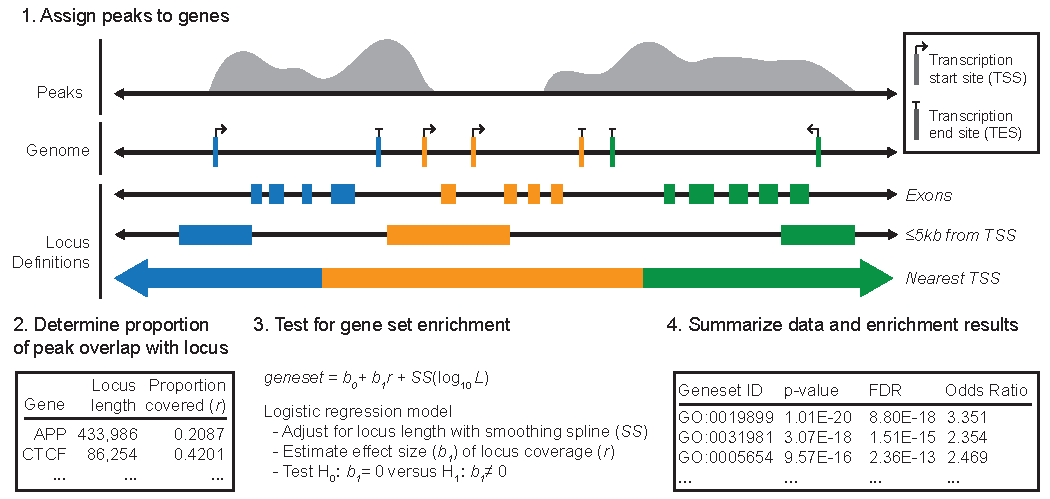
\includegraphics[width=1\textwidth]{chap2figs/figure2_1.pdf}
\caption[Broad-Enrich functions in four steps.]
{
% Rackham requires the figure list title matches the first sentence, so repeat that sentence here
\textbf{Broad-Enrich functions in four steps.}
(1) The user selects a gene locus definition (exons, $\leq$ 5kb, and nearest TSS are shown). (2) The proportion of each gene locus covered by ChIP-seq peaks from a given HM, or otherwise derived genomic regions, is determined. (3) For each gene set to be tested, logistic regression is performed using the model shown, where geneset refers to the binary vector of gene set membership, r refers to the vector of proportions of the gene loci covered by all peaks overlapping the respective loci, SS is a binomial cubic smoothing spline which corrects for any locus length bias, and L is a vector of gene locus lengths. (4) P-values for enrichment or depletion are adjusted for multiple testing and users are provided summarized functional enrichment results, peak to gene loci assignments, and diagnostic plots.
}
\label{chap2:fig:1}
\end{figure}

\newpage

\begin{figure}[ht!]
\centering
% manually adjust the width of the figure
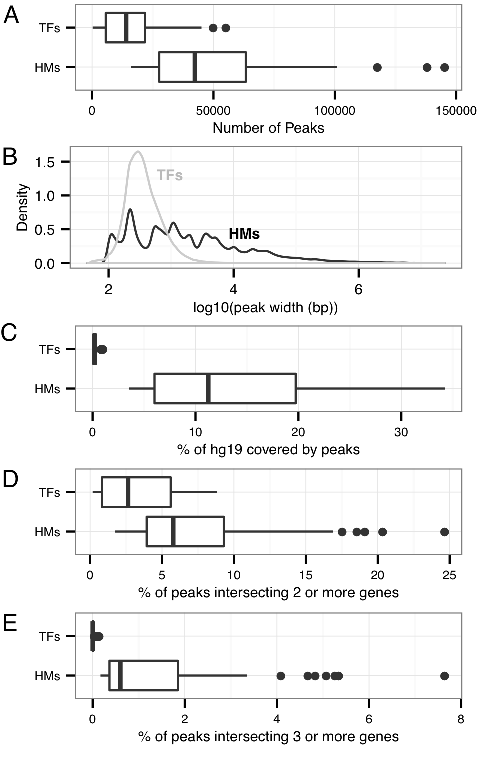
\includegraphics[width=0.7\textwidth]{chap2figs/figure2_2.pdf}
\caption[Histone (HM) and transcription-factor (TF) based peak sets exhibit several different properties.]
{
% Rackham requires the figure list title matches the first sentence, so repeat that sentence here
\textbf{Histone (HM) and transcription-factor (TF) based peak sets exhibit several different properties.} Observed over 100 TF and 55 HM ENCODE ChIP-seq datasets. (A) There tends to be more peaks in HM  experiments (median = 42,330) compared to TF experiments (median = 14,040). (B) The peak width distributions are significantly different. HM peaks (black) tend to be broad and highly variable (median = 1,255 bp, sd = 483,279 bp), while TF peaks (gray) tend to be narrow and less variable (median = 330 bp, sd = 560 bp). (C) HM peaks consistently cover a greater percentage of hg19 (median = 11.25\%) than TF peaks (median = 0.16\%). (D) The percentage of peaks covering two or more gene loci also tends to be higher for HMs (median = 5.78\%) than for TFs (median = 2.64\%). (E) The same is true of peaks covering three or more gene loci (median = 0.6\% and 0\%, respectively). Both (D) and (E) use the nearest TSS definition.
}
\label{chap2:fig:2}
\end{figure}

\newpage

\begin{figure}[ht!]
\centering
% manually adjust the width of the figure
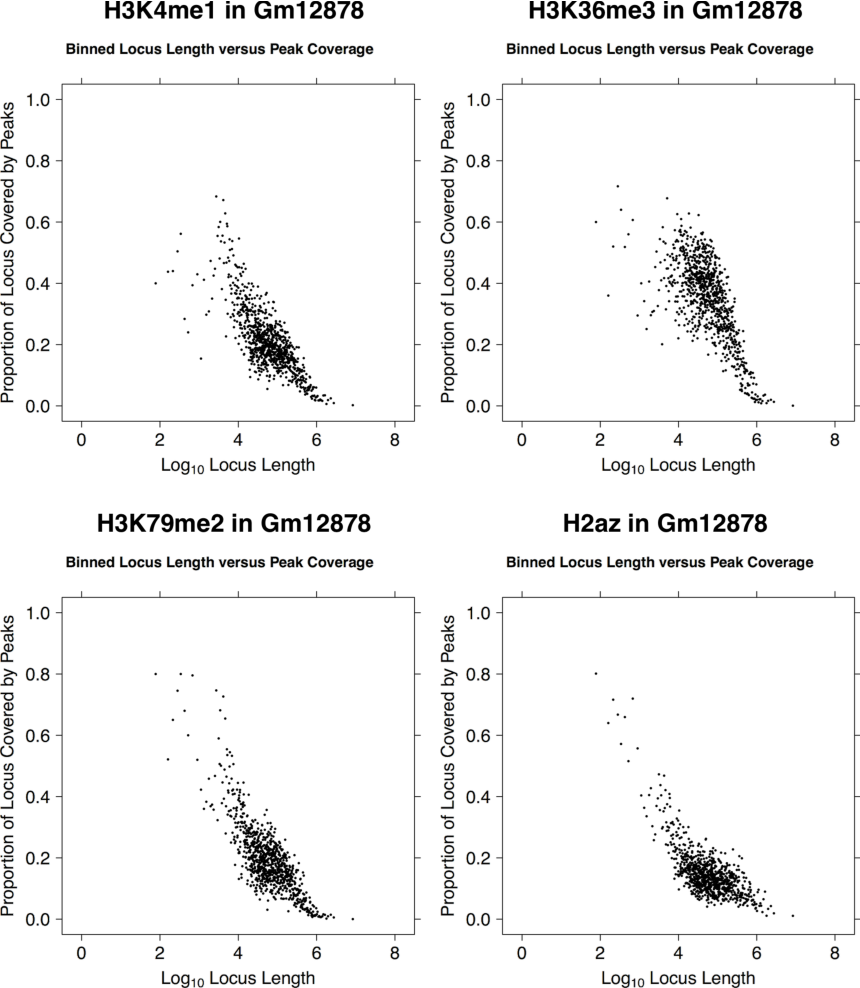
\includegraphics[width=0.7\textwidth]{chap2figs/figure2_3.pdf}
\caption[The relationship between gene locus length and the percentage of the locus covered by a peak.]
{
% Rackham requires the figure list title matches the first sentence, so repeat that sentence here
\textbf{The relationship between gene locus length and the percentage of the locus covered by a peak.} For selected HM datasets in cell line GM12878 using the nearest TSS locus definition. For visualization purposes, genes were binned in groups of 25 by their locus length, such that each point represents the average of 25 genes. There tends to be a strong negative correlation between log10 locus length and the proportion of the locus covered by a peak.
}
\label{chap2:fig:3}
\end{figure}

\newpage

\begin{figure}[ht!]
\centering
% manually adjust the width of the figure
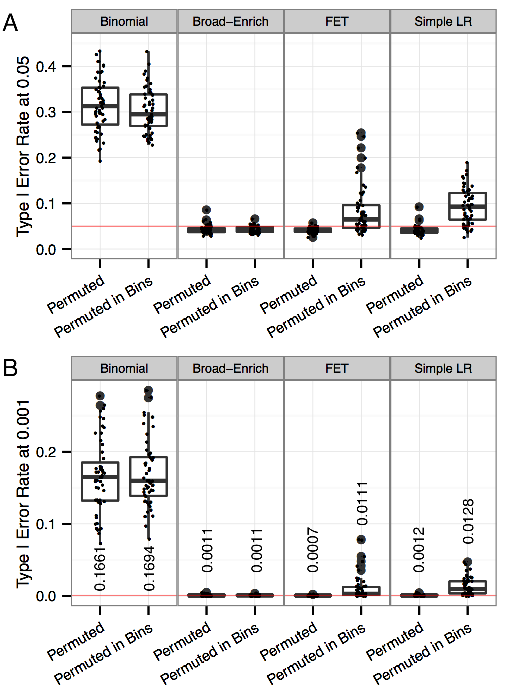
\includegraphics[width=0.7\textwidth]{chap2figs/figure2_4.pdf}
\caption[Type I error rates for enrichment tests.]
{
% Rackham requires the figure list title matches the first sentence, so repeat that sentence here
\textbf{Type I error rates for enrichment tests.} Type I error rates of the binomial-based test, Broad-Enrich, the simple LR model, and Fisher's exact test under the two permutation scenarios with the nearest TSS locus definition. Each point represents 1 of the 55 HM datasets. (A) At $\alpha = 0.05$  (red line), we find inflated type I error for the binomial test under both permutation scenarios, the correct error rate for Broad-Enrich, and the correct error rate for permutations eliminating length bias but often inflated error for permutations preserving length bias for both the simple LR model and Fisher's exact test. (B) At $\alpha = 0.001$ (red line), we observe results similar to $\alpha = 0.05$. Mean error rates are given inset.
}
\label{chap2:fig:4}
\end{figure}

\newpage

\begin{figure}[ht!]
\centering
% manually adjust the width of the figure
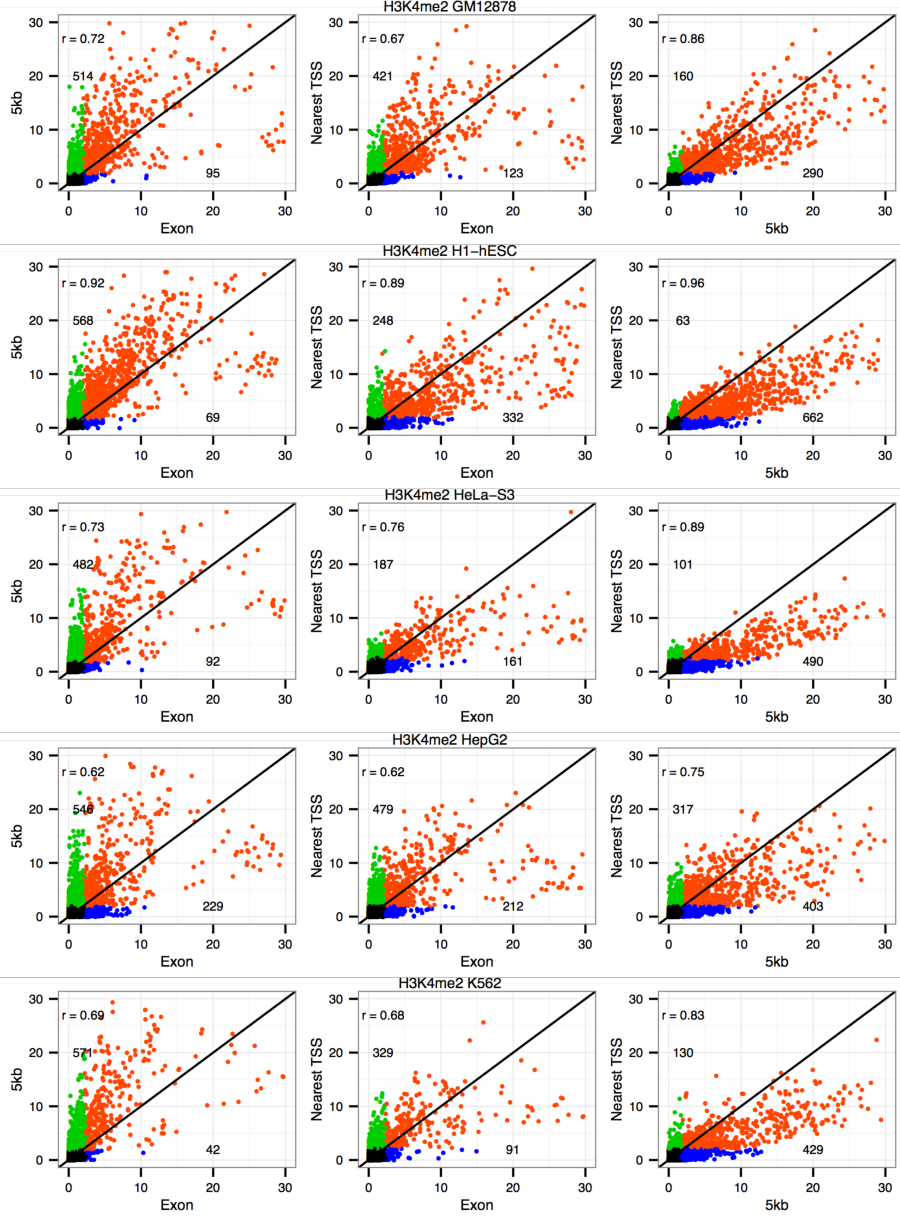
\includegraphics[width=0.8\textwidth]{chap2figs/figure2_5.pdf}
\caption[H3K4me2 enrichment signal for different locus definitions.]
{
% Rackham requires the figure list title matches the first sentence, so repeat that sentence here
\textbf{H3K4me2 enrichment signal for different locus definitions.} Enrichment signal (-log10 p-value) comparing nearest TSS, $\leq$ 5kb from TSS, and exons locus definitions for H3K4me2 across 5 cell lines. H3K4me2 tends to occur in the proximal promoter, and $\leq$ 5kb tends to perform better versus nearest TSS and versus exons. Axes limits are constrained for visual clarity. Pearson correlation coefficient of all p-values (including those outside axis limits) is reported inset. Green points are unique enrichments ($\beta_1 > 0$ and $FDR < 0.05$) for the locus definition on the y-axis (number is inset), blue points are unique enrichments for the locus definitions on the x-axis (number is inset), orange points are enriched in both, and black in neither.
}
\label{chap2:fig:5}
\end{figure}

\newpage

\begin{figure}[ht!]
\centering
% manually adjust the width of the figure
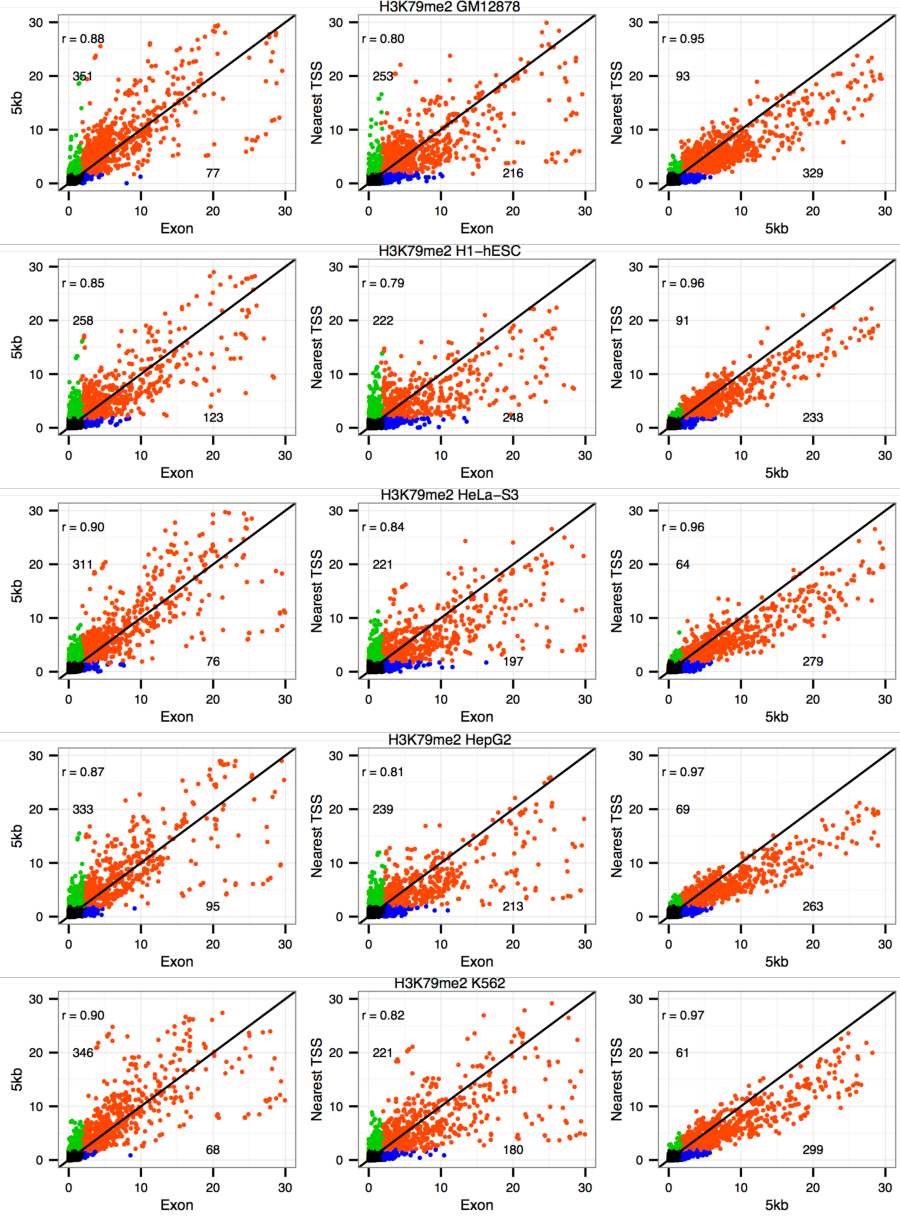
\includegraphics[width=0.8\textwidth]{chap2figs/figure2_6.pdf}
\caption[H3K79me2 enrichment signal for different locus definitions.]
{
% Rackham requires the figure list title matches the first sentence, so repeat that sentence here
\textbf{H3K79me2 enrichment signal for different locus definitions.} Enrichment signal (-log10 p-value) comparing nearest TSS, $\leq$ 5kb from TSS, and exons locus definitions for H3K79me2 across 5 cell lines. H3K79me2 preferentially occurs at the 5' end of genes, which is best captured by the $\leq$ 5kb locus definition, and $\leq$ 5kb performs better versus both nearest TSS and exons. Axes limits are constrained for visual clarity. Pearson correlation coefficient of all p-values (including those outside axis limits) is reported inset. Green points are unique enrichments ($\beta_1 > 0$ and $FDR < 0.05$) for the locus definition on the y-axis (number is inset), blue points are unique enrichments for the locus definitions on the x-axis (number is inset), orange points are enriched in both, and black in neither.
}
\label{chap2:fig:6}
\end{figure}

\newpage

\begin{figure}[ht!]
\centering
% manually adjust the width of the figure
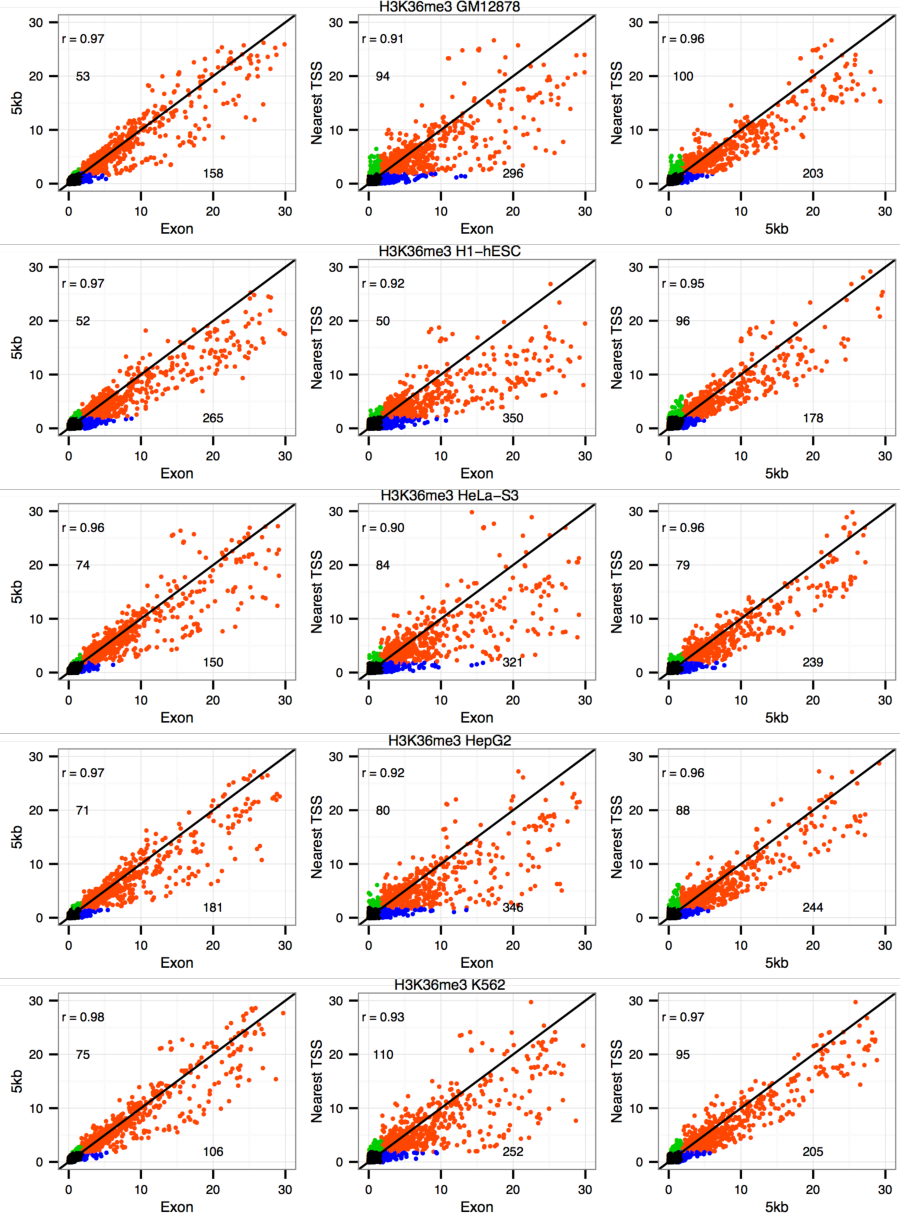
\includegraphics[width=0.8\textwidth]{chap2figs/figure2_7.pdf}
\caption[H3K36me3 enrichment signal for different locus definitions.]
{
% Rackham requires the figure list title matches the first sentence, so repeat that sentence here
\textbf{H3K36me3 enrichment signal for different locus definitions.} Enrichment signal (-log10 p-value) comparing nearest TSS, $\leq$ 5kb from TSS, and exons locus definitions for H3K36me3 across 5 cell lines. H3K36me3 preferentially occurs near the 3' end of genes, perhaps out of reach of the $\leq$ 5kb locus definition. The exons definition tends to provide stronger enrichment signal versus both nearest TSS and $\leq$ 5kb. Axes limits are constrained for visual clarity. Pearson correlation coefficient of all p-values (including those outside axis limits) is reported inset. Green points are unique enrichments ($\beta_1 > 0$ and $FDR < 0.05$) for the locus definition on the y-axis (number is inset), blue points are unique enrichments for the locus definitions on the x-axis (number is inset), orange points are enriched in both, and black in neither.
}
\label{chap2:fig:7}
\end{figure}

\newpage

\begin{figure}[ht!]
\centering
% manually adjust the width of the figure
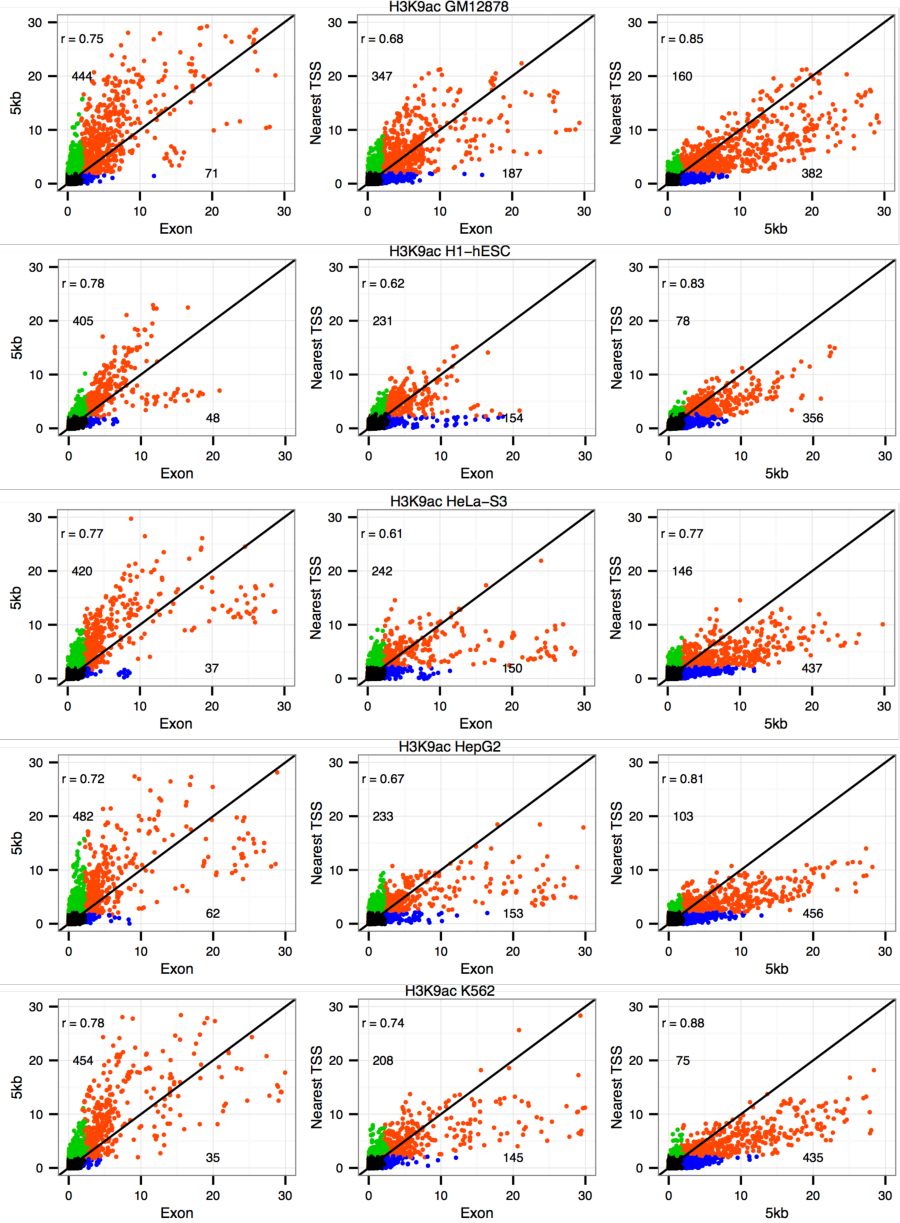
\includegraphics[width=0.8\textwidth]{chap2figs/figure2_8.pdf}
\caption[H3K9ac enrichment signal for different locus definitions.]
{
% Rackham requires the figure list title matches the first sentence, so repeat that sentence here
\textbf{H3K9ac enrichment signal for different locus definitions.} Enrichment signal (-log10 p-value) comparing nearest TSS, $\leq$ 5kb from TSS, and exons locus definitions for H3K9ac across 5 cell lines. Overall, $\leq$ 5kb and tends to perform better versus nearest TSS and versus exons. Note, for some gene sets exons clearly outperforms $\leq$ 5kb. This occurs specifically in embryonic stem cells and HeLa-S3 cells. Axes limits are constrained for visual clarity. Pearson correlation coefficient of all p-values (including those outside axis limits) is reported inset. Green points are unique enrichments ($\beta_1 > 0$ and $FDR < 0.05$) for the locus definition on the y-axis (number is inset), blue points are unique enrichments for the locus definitions on the x-axis (number is inset), orange points are enriched in both, and black in neither.
}
\label{chap2:fig:8}
\end{figure}

\newpage

\begin{figure}[ht!]
\centering
% manually adjust the width of the figure
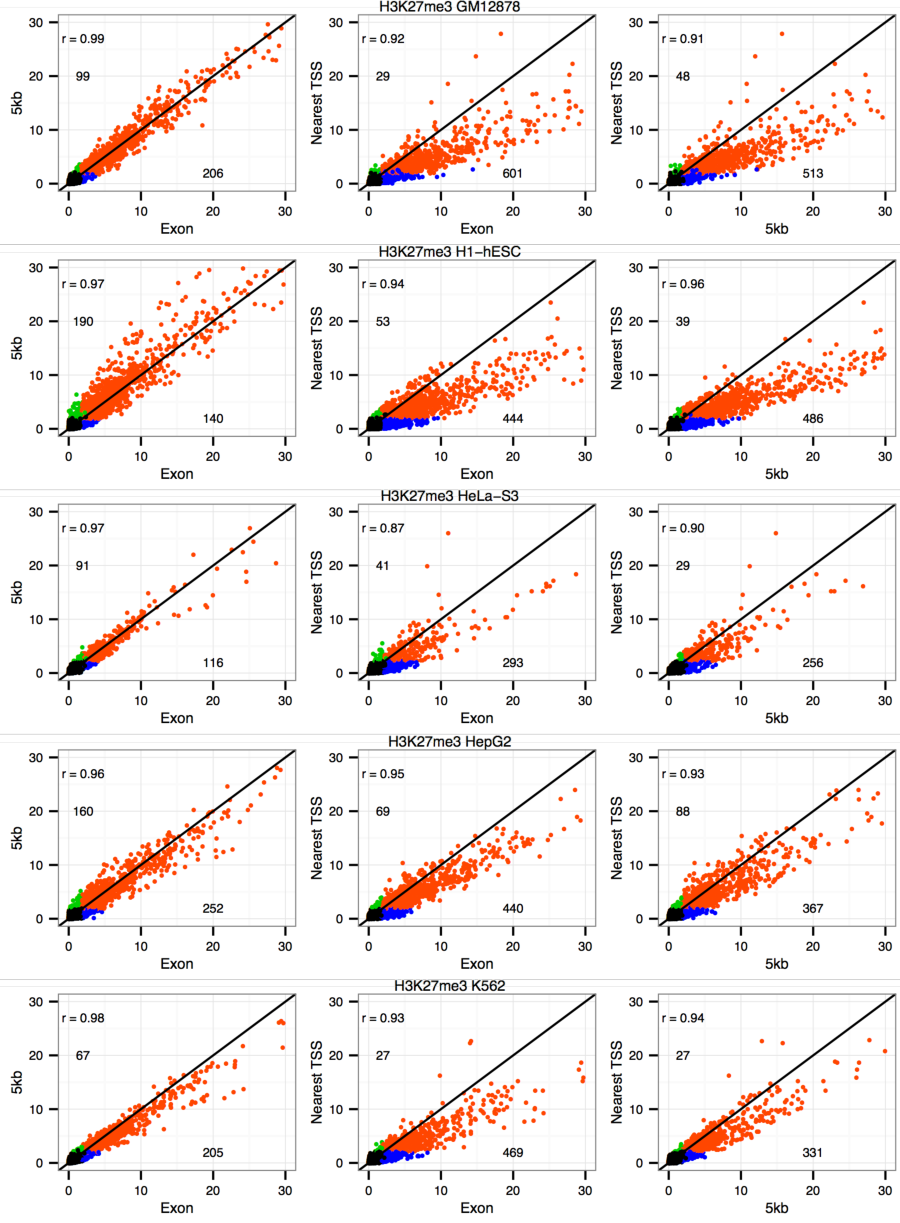
\includegraphics[width=0.8\textwidth]{chap2figs/figure2_9.pdf}
\caption[H3K27me3 enrichment signal for different locus definitions.]
{
% Rackham requires the figure list title matches the first sentence, so repeat that sentence here
\textbf{H3K27me3 enrichment signal for different locus definitions.} Enrichment signal (-log10 p-value) comparing nearest TSS, $\leq$ 5kb from TSS, and exons locus definitions for H3K27me3 across 5 cell lines. While both $\leq$ 5kb and exons perform better than nearest TSS, exons tends to perform slightly better than $\leq$ 5kb in all cell lines with the exception of H1-hESC. This could indicate a different regulatory regime for H3K27me3 in embryonic stem cells compared to the other, more differentiated, cell lines. Axes limits are constrained for visual clarity. Pearson correlation coefficient of all p-values (including those outside axis limits) is reported inset. Green points are unique enrichments ($\beta_1 > 0$ and $FDR < 0.05$) for the locus definition on the y-axis (number is inset), blue points are unique enrichments for the locus definitions on the x-axis (number is inset), orange points are enriched in both, and black in neither.
}
\label{chap2:fig:9}
\end{figure}

\newpage

\begin{figure}[ht!]
\centering
% manually adjust the width of the figure
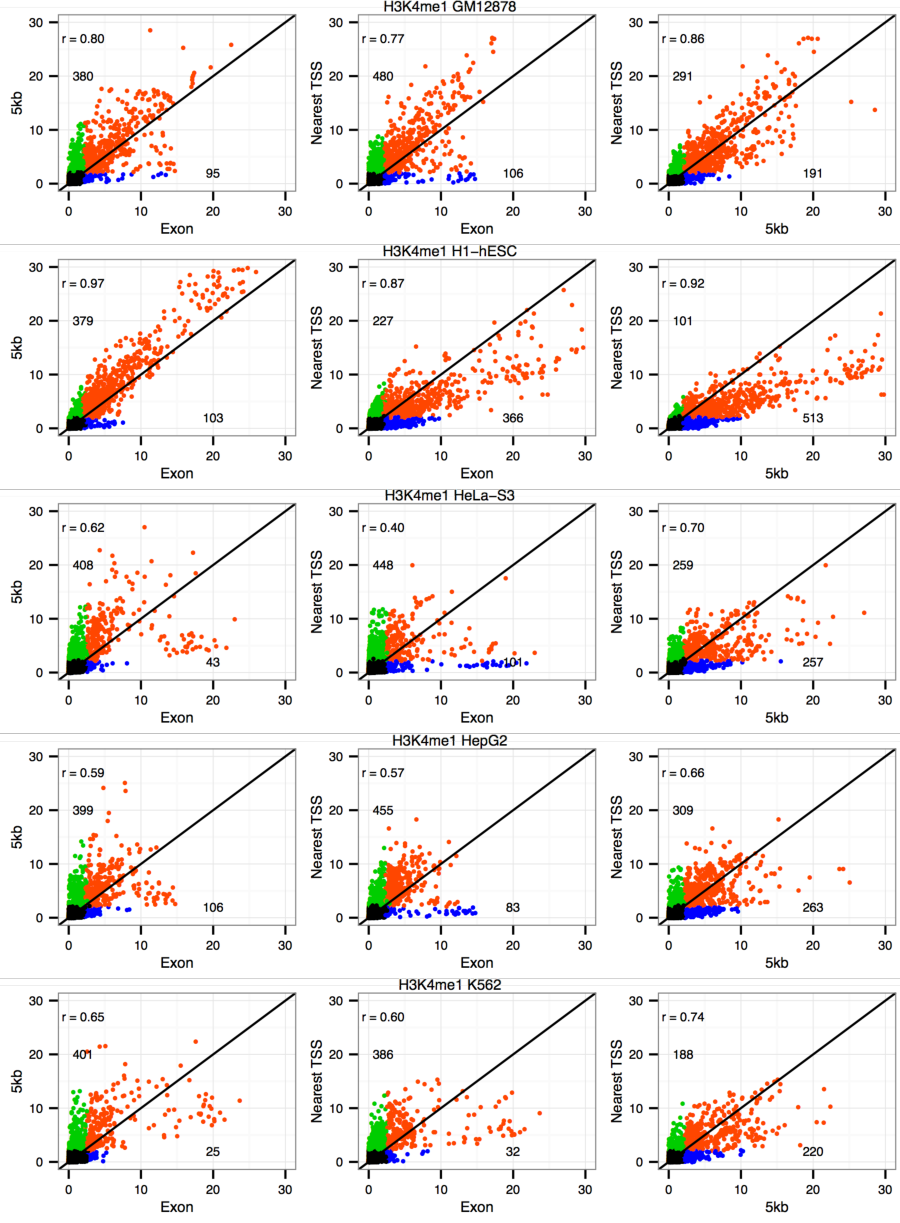
\includegraphics[width=0.8\textwidth]{chap2figs/figure2_10.pdf}
\caption[H3K4me1 enrichment signal for different locus definitions.]
{
% Rackham requires the figure list title matches the first sentence, so repeat that sentence here
\textbf{H3K4me1 enrichment signal for different locus definitions.} Enrichment signal (-log10 p-value) comparing nearest TSS, $\leq$ 5kb from TSS, and exons locus definitions for H3K4me1 across 5 cell lines. There is no clearly better performing locus definition across the cell lines. Nearest TSS performs better for GM12878 and HepG2, while $\leq$ 5kb performs better in H1-hESC, HeLa-S3, and K562. Recall, nearest TSS includes enhancer regions, whereas $\leq$ 5kb only includes proximal promoter regions. Consequently, the enrichment results may be a reflection of more long-range regulatory architecture in GM12878 and HepG2 versus more short-range architecture in the remaining cell lines. Axes limits are constrained for visual clarity. Pearson correlation coefficient of all p-values (including those outside axis limits) is reported inset. Green points are unique enrichments ($\beta_1 > 0$ and $FDR < 0.05$) for the locus definition on the y-axis (number is inset), blue points are unique enrichments for the locus definitions on the x-axis (number is inset), orange points are enriched in both, and black in neither.
}
\label{chap2:fig:10}
\end{figure}

\clearpage
\section*{Tables}
\begin{table}[!ht]
\tiny
\centering
\begin{tabular}{ll|ll|ll|ll|ll}
\multicolumn{2}{l}{}                                        & \multicolumn{2}{c}{{\color[HTML]{000000} \textbf{Binomial}}}                                                               & \multicolumn{2}{c}{\textbf{Broad-Enrich}}                                    & \multicolumn{2}{c}{\textbf{Broad-Enrich NS}}                                   & \multicolumn{2}{c}{\textbf{FET}}                                               \\
\multicolumn{1}{c}{\textbf{Histone}} & \multicolumn{1}{c}{\textbf{Cell Line}} & \multicolumn{1}{c}{{\color[HTML]{000000} \textbf{Permuted}}} & \multicolumn{1}{c}{{\color[HTML]{000000} \textbf{In Bins}}} & \multicolumn{1}{c}{\textbf{Permuted}} & \multicolumn{1}{c}{\textbf{In Bins}} & \multicolumn{1}{c}{\textbf{Permuted}} & \multicolumn{1}{c}{\textbf{In Bins}}   & \multicolumn{1}{c}{\textbf{Permuted}} & \multicolumn{1}{c}{\textbf{In Bins}}   \\\hline
H2az                                 & Gm12878                                & {\color[HTML]{CB0000} \textbf{0.3092}}                       & {\color[HTML]{CB0000} \textbf{0.3901}}                      & 0.0411                                & 0.0463                               & 0.0476                                & \textbf{0.0716}                        & 0.0409                                & \textbf{0.0603}                        \\
H3k27ac                              & Gm12878                                & {\color[HTML]{CB0000} \textbf{0.3127}}                       & {\color[HTML]{CB0000} \textbf{0.3368}}                      & 0.0527                                & 0.0352                               & 0.0426                                & {\color[HTML]{CB0000} \textbf{0.1295}} & 0.0387                                & 0.0398                                 \\
H3k27me3                             & Gm12878                                & {\color[HTML]{CB0000} \textbf{0.2195}}                       & {\color[HTML]{CB0000} \textbf{0.2409}}                      & 0.0494                                & 0.0444                               & 0.0398                                & {\color[HTML]{CB0000} \textbf{0.1105}} & 0.0385                                & {\color[HTML]{CB0000} \textbf{0.1401}} \\
H3k36me3                             & Gm12878                                & {\color[HTML]{CB0000} \textbf{0.1923}}                       & {\color[HTML]{CB0000} \textbf{0.2369}}                      & 0.0455                                & 0.0320                               & 0.0381                                & {\color[HTML]{CB0000} \textbf{0.1375}} & 0.0411                                & 0.0307                                 \\
H3k4me1                              & Gm12878                                & {\color[HTML]{CB0000} \textbf{0.3749}}                       & {\color[HTML]{CB0000} \textbf{0.4045}}                      & 0.0357                                & 0.0398                               & 0.0313                                & {\color[HTML]{CB0000} \textbf{0.1558}} & 0.0422                                & \textbf{0.0650}                        \\
H3k4me2                              & Gm12878                                & {\color[HTML]{CB0000} \textbf{0.3205}}                       & {\color[HTML]{CB0000} \textbf{0.3490}}                      & \textbf{0.0855}                       & 0.0396                               & 0.0437                                & {\color[HTML]{CB0000} \textbf{0.1031}} & 0.0326                                & \textbf{0.0751}                        \\
H3k4me3                              & Gm12878                                & {\color[HTML]{CB0000} \textbf{0.4110}}                       & {\color[HTML]{CB0000} \textbf{0.3033}}                      & 0.0365                                & 0.0483                               & 0.0479                                & \textbf{0.0790}                        & 0.0379                                & \textbf{0.0675}                        \\
H3k79me2                             & Gm12878                                & {\color[HTML]{CB0000} \textbf{0.2998}}                       & {\color[HTML]{CB0000} \textbf{0.2650}}                      & 0.0346                                & 0.0535                               & 0.0365                                & 0.0426                                 & 0.0402                                & 0.0431                                 \\
H3k9ac                               & Gm12878                                & {\color[HTML]{CB0000} \textbf{0.2759}}                       & {\color[HTML]{CB0000} \textbf{0.3087}}                      & 0.0446                                & 0.0324                               & 0.0498                                & \textbf{0.0725}                        & 0.0476                                & 0.0426                                 \\
H3k9me3                              & Gm12878                                & {\color[HTML]{CB0000} \textbf{0.3199}}                       & {\color[HTML]{CB0000} \textbf{0.3427}}                      & 0.0309                                & 0.0361                               & 0.0357                                & \textbf{0.0642}                        & 0.0407                                & {\color[HTML]{CB0000} \textbf{0.2215}} \\
H4k20me1                             & Gm12878                                & {\color[HTML]{CB0000} \textbf{0.2422}}                       & {\color[HTML]{CB0000} \textbf{0.2689}}                      & 0.0383                                & 0.0331                               & 0.0346                                & {\color[HTML]{CB0000} \textbf{0.1108}} & 0.0346                                & \textbf{0.0781}                        \\
H2az                                 & H1hesc                                 & {\color[HTML]{CB0000} \textbf{0.3869}}                       & {\color[HTML]{CB0000} \textbf{0.2950}}                      & 0.0372                                & 0.0402                               & 0.0392                                & \textbf{0.0646}                        & 0.0398                                & \textbf{0.0814}                        \\
H3k27ac                              & H1hesc                                 & {\color[HTML]{CB0000} \textbf{0.2678}}                       & {\color[HTML]{CB0000} \textbf{0.3024}}                      & 0.0415                                & 0.0490                               & 0.0392                                & \textbf{0.0731}                        & 0.0437                                & \textbf{0.0907}                        \\
H3k27me3                             & H1hesc                                 & {\color[HTML]{CB0000} \textbf{0.2568}}                       & {\color[HTML]{CB0000} \textbf{0.2328}}                      & 0.0368                                & 0.0398                               & 0.0352                                & \textbf{0.0883}                        & 0.0385                                & {\color[HTML]{CB0000} \textbf{0.1678}} \\
H3k36me3                             & H1hesc                                 & {\color[HTML]{CB0000} \textbf{0.2172}}                       & {\color[HTML]{CB0000} \textbf{0.2280}}                      & 0.0403                                & 0.0342                               & 0.0477                                & {\color[HTML]{CB0000} \textbf{0.1297}} & 0.0476                                & 0.0477                                 \\
H3k4me1                              & H1hesc                                 & {\color[HTML]{CB0000} \textbf{0.3327}}                       & {\color[HTML]{CB0000} \textbf{0.2857}}                      & 0.0405                                & 0.0501                               & 0.0333                                & {\color[HTML]{CB0000} \textbf{0.1584}} & 0.0392                                & {\color[HTML]{CB0000} \textbf{0.1005}} \\
H3k4me2                              & H1hesc                                 & {\color[HTML]{CB0000} \textbf{0.3571}}                       & {\color[HTML]{CB0000} \textbf{0.3174}}                      & 0.0522                                & \textbf{0.0661}                      & 0.0385                                & 0.0557                                 & 0.0468                                & \textbf{0.0818}                        \\
H3k4me3                              & H1hesc                                 & {\color[HTML]{CB0000} \textbf{0.2361}}                       & {\color[HTML]{CB0000} \textbf{0.2487}}                      & 0.0501                                & 0.0305                               & 0.0339                                & 0.0522                                 & 0.0337                                & 0.0540                                 \\
H3k79me2                             & H1hesc                                 & {\color[HTML]{CB0000} \textbf{0.3087}}                       & {\color[HTML]{CB0000} \textbf{0.3155}}                      & \textbf{0.0644}                       & 0.0376                               & 0.0318                                & 0.0398                                 & 0.0396                                & \textbf{0.0642}                        \\
H3k9ac                               & H1hesc                                 & {\color[HTML]{CB0000} \textbf{0.3190}}                       & {\color[HTML]{CB0000} \textbf{0.2887}}                      & 0.0370                                & 0.0487                               & \textbf{0.0629}                       & \textbf{0.0927}                        & 0.0435                                & \textbf{0.0968}                        \\
H3k9me3                              & H1hesc                                 & {\color[HTML]{CB0000} \textbf{0.2328}}                       & {\color[HTML]{CB0000} \textbf{0.2826}}                      & 0.0427                                & 0.0396                               & 0.0241                                & 0.0509                                 & 0.0494                                & {\color[HTML]{CB0000} \textbf{0.2469}} \\
H4k20me1                             & H1hesc                                 & {\color[HTML]{CB0000} \textbf{0.3205}}                       & {\color[HTML]{CB0000} \textbf{0.2509}}                      & 0.0444                                & 0.0518                               & 0.0472                                & \textbf{0.0831}                        & 0.0377                                & {\color[HTML]{CB0000} \textbf{0.1062}} \\
H2az                                 & Helas3                                 & {\color[HTML]{CB0000} \textbf{0.3886}}                       & {\color[HTML]{CB0000} \textbf{0.3397}}                      & 0.0353                                & 0.0344                               & 0.0294                                & 0.0252                                 & 0.0394                                & 0.0548                                 \\
H3k27ac                              & Helas3                                 & {\color[HTML]{CB0000} \textbf{0.3494}}                       & {\color[HTML]{CB0000} \textbf{0.2800}}                      & 0.0335                                & 0.0431                               & 0.0374                                & {\color[HTML]{CB0000} \textbf{0.1166}} & 0.0361                                & 0.0505                                 \\
H3k27me3                             & Helas3                                 & {\color[HTML]{CB0000} \textbf{0.2415}}                       & {\color[HTML]{CB0000} \textbf{0.2776}}                      & 0.0437                                & 0.0446                               & 0.0446                                & {\color[HTML]{CB0000} \textbf{0.1121}} & 0.0453                                & {\color[HTML]{CB0000} \textbf{0.1223}} \\
H3k36me3                             & Helas3                                 & {\color[HTML]{CB0000} \textbf{0.2522}}                       & {\color[HTML]{CB0000} \textbf{0.2778}}                      & 0.0389                                & 0.0453                               & 0.0357                                & \textbf{0.0972}                        & 0.0472                                & \textbf{0.0727}                        \\
H3k4me1                              & Helas3                                 & {\color[HTML]{CB0000} \textbf{0.4260}}                       & {\color[HTML]{CB0000} \textbf{0.4325}}                      & 0.0442                                & 0.0357                               & 0.0522                                & {\color[HTML]{CB0000} \textbf{0.1195}} & 0.0383                                & \textbf{0.0648}                        \\
H3k4me2                              & Helas3                                 & {\color[HTML]{CB0000} \textbf{0.3681}}                       & {\color[HTML]{CB0000} \textbf{0.3429}}                      & \textbf{0.0616}                       & 0.0561                               & 0.0355                                & \textbf{0.0872}                        & 0.0254                                & \textbf{0.0738}                        \\
H3k4me3                              & Helas3                                 & {\color[HTML]{CB0000} \textbf{0.2950}}                       & {\color[HTML]{CB0000} \textbf{0.3164}}                      & 0.0348                                & 0.0377                               & 0.0357                                & \textbf{0.0742}                        & 0.0442                                & 0.0476                                 \\
H3k79me2                             & Helas3                                 & {\color[HTML]{CB0000} \textbf{0.3436}}                       & {\color[HTML]{CB0000} \textbf{0.3038}}                      & 0.0377                                & 0.0511                               & 0.0400                                & \textbf{0.0725}                        & 0.0461                                & \textbf{0.0620}                        \\
H3k9ac                               & Helas3                                 & {\color[HTML]{CB0000} \textbf{0.2974}}                       & {\color[HTML]{CB0000} \textbf{0.2702}}                      & 0.0457                                & 0.0348                               & 0.0387                                & 0.0550                                 & 0.0483                                & 0.0520                                 \\
H3k9me3                              & Helas3                                 & {\color[HTML]{CB0000} \textbf{0.3035}}                       & {\color[HTML]{CB0000} \textbf{0.2470}}                      & 0.0377                                & 0.0437                               & 0.0311                                & \textbf{0.0674}                        & 0.0287                                & {\color[HTML]{CB0000} \textbf{0.1997}} \\
H4k20me1                             & Helas3                                 & {\color[HTML]{CB0000} \textbf{0.2953}}                       & {\color[HTML]{CB0000} \textbf{0.3830}}                      & 0.0403                                & 0.0353                               & 0.0357                                & \textbf{0.0664}                        & 0.0390                                & {\color[HTML]{CB0000} \textbf{0.1255}} \\
H2az                                 & Hepg2                                  & {\color[HTML]{CB0000} \textbf{0.3249}}                       & {\color[HTML]{CB0000} \textbf{0.2846}}                      & 0.0368                                & 0.0544                               & 0.0361                                & \textbf{0.0644}                        & 0.0409                                & 0.0555                                 \\
H3k27ac                              & Hepg2                                  & {\color[HTML]{CB0000} \textbf{0.3383}}                       & {\color[HTML]{CB0000} \textbf{0.3216}}                      & 0.0420                                & 0.0329                               & 0.0439                                & {\color[HTML]{CB0000} \textbf{0.1255}} & 0.0461                                & 0.0370                                 \\
H3k27me3                             & Hepg2                                  & {\color[HTML]{CB0000} \textbf{0.3014}}                       & {\color[HTML]{CB0000} \textbf{0.2859}}                      & 0.0439                                & 0.0509                               & 0.0476                                & \textbf{0.0951}                        & 0.0377                                & \textbf{0.0816}                        \\
H3k36me3                             & Hepg2                                  & {\color[HTML]{CB0000} \textbf{0.2976}}                       & {\color[HTML]{CB0000} \textbf{0.2459}}                      & 0.0427                                & 0.0429                               & 0.0376                                & {\color[HTML]{CB0000} \textbf{0.1893}} & 0.0477                                & 0.0392                                 \\
H3k4me1                              & Hepg2                                  & {\color[HTML]{CB0000} \textbf{0.4030}}                       & {\color[HTML]{CB0000} \textbf{0.3625}}                      & 0.0453                                & 0.0437                               & \textbf{0.0659}                       & {\color[HTML]{CB0000} \textbf{0.1719}} & 0.0392                                & \textbf{0.0949}                        \\
H3k4me2                              & Hepg2                                  & {\color[HTML]{CB0000} \textbf{0.4334}}                       & {\color[HTML]{CB0000} \textbf{0.3740}}                      & 0.0292                                & 0.0481                               & 0.0346                                & {\color[HTML]{CB0000} \textbf{0.1070}} & 0.0426                                & \textbf{0.0835}                        \\
H3k4me3                              & Hepg2                                  & {\color[HTML]{CB0000} \textbf{0.3531}}                       & {\color[HTML]{CB0000} \textbf{0.3311}}                      & 0.0455                                & 0.0540                               & 0.0446                                & {\color[HTML]{CB0000} \textbf{0.1386}} & 0.0366                                & 0.0444                                 \\
H3k79me2                             & Hepg2                                  & {\color[HTML]{CB0000} \textbf{0.3292}}                       & {\color[HTML]{CB0000} \textbf{0.2635}}                      & 0.0446                                & 0.0363                               & \textbf{0.0922}                       & 0.0431                                 & 0.0400                                & 0.0514                                 \\
H3k9ac                               & Hepg2                                  & {\color[HTML]{CB0000} \textbf{0.3298}}                       & {\color[HTML]{CB0000} \textbf{0.3118}}                      & 0.0581                                & 0.0390                               & 0.0381                                & 0.0377                                 & 0.0461                                & 0.0413                                 \\
H3k9me3                              & Hepg2                                  & {\color[HTML]{CB0000} \textbf{0.2837}}                       & {\color[HTML]{CB0000} \textbf{0.3370}}                      & 0.0470                                & 0.0435                               & 0.0313                                & 0.0575                                 & 0.0346                                & \textbf{0.2543}                        \\
H4k20me1                             & Hepg2                                  & {\color[HTML]{CB0000} \textbf{0.2552}}                       & {\color[HTML]{CB0000} \textbf{0.2720}}                      & 0.0455                                & 0.0411                               & 0.0411                                & \textbf{0.0981}                        & 0.0522                                & {\color[HTML]{CB0000} \textbf{0.1195}} \\
H2az                                 & K562                                   & {\color[HTML]{CB0000} \textbf{0.3647}}                       & {\color[HTML]{CB0000} \textbf{0.3705}}                      & 0.0361                                & 0.0376                               & 0.0466                                & \textbf{0.0964}                        & 0.0363                                & 0.0563                                 \\
H3k27ac                              & K562                                   & {\color[HTML]{CB0000} \textbf{0.4110}}                       & {\color[HTML]{CB0000} \textbf{0.3394}}                      & 0.0287                                & 0.0405                               & 0.0461                                & {\color[HTML]{CB0000} \textbf{0.1442}} & 0.0396                                & 0.0513                                 \\
H3k27me3                             & K562                                   & {\color[HTML]{CB0000} \textbf{0.2909}}                       & {\color[HTML]{CB0000} \textbf{0.2715}}                      & 0.0387                                & 0.0533                               & 0.0374                                & {\color[HTML]{CB0000} \textbf{0.1107}} & 0.0492                                & {\color[HTML]{CB0000} \textbf{0.1355}} \\
H3k36me3                             & K562                                   & {\color[HTML]{CB0000} \textbf{0.2691}}                       & {\color[HTML]{CB0000} \textbf{0.2541}}                      & 0.0518                                & 0.0550                               & 0.0453                                & {\color[HTML]{CB0000} \textbf{0.1273}} & 0.0359                                & 0.0435                                 \\
H3k4me1                              & K562                                   & {\color[HTML]{CB0000} \textbf{0.4010}}                       & {\color[HTML]{CB0000} \textbf{0.3546}}                      & 0.0366                                & 0.0435                               & 0.0429                                & {\color[HTML]{CB0000} \textbf{0.1628}} & 0.0383                                & 0.0402                                 \\
H3k4me2                              & K562                                   & {\color[HTML]{CB0000} \textbf{0.3871}}                       & {\color[HTML]{CB0000} \textbf{0.3568}}                      & 0.0468                                & 0.0409                               & 0.0400                                & {\color[HTML]{CB0000} \textbf{0.1301}} & 0.0300                                & 0.0326                                 \\
H3k4me3                              & K562                                   & {\color[HTML]{CB0000} \textbf{0.3451}}                       & {\color[HTML]{CB0000} \textbf{0.2907}}                      & 0.0485                                & 0.0394                               & 0.0370                                & {\color[HTML]{CB0000} \textbf{0.1158}} & 0.0439                                & 0.0452                                 \\
H3k79me2                             & K562                                   & {\color[HTML]{CB0000} \textbf{0.2659}}                       & {\color[HTML]{CB0000} \textbf{0.2432}}                      & 0.0377                                & 0.0470                               & 0.0498                                & 0.0457                                 & 0.0289                                & 0.0389                                 \\
H3k9ac                               & K562                                   & {\color[HTML]{CB0000} \textbf{0.3531}}                       & {\color[HTML]{CB0000} \textbf{0.3259}}                      & 0.0339                                & 0.0492                               & 0.0405                                & \textbf{0.0659}                        & 0.0346                                & 0.0387                                 \\
H3k9me3                              & K562                                   & {\color[HTML]{CB0000} \textbf{0.2807}}                       & {\color[HTML]{CB0000} \textbf{0.2400}}                      & 0.0361                                & 0.0372                               & 0.0370                                & 0.0509                                 & 0.0372                                & {\color[HTML]{CB0000} \textbf{0.1784}} \\
H4k20me1                             & K562                                   & {\color[HTML]{CB0000} \textbf{0.2446}}                       & {\color[HTML]{CB0000} \textbf{0.2837}}                      & 0.0540                                & 0.0390                               & 0.0426                                & {\color[HTML]{CB0000} \textbf{0.1447}} & 0.0575                                & \textbf{0.0894}
\end{tabular}
\normalsize
\caption[Type I error rate estimates for Broad-Enrich, the binomial-based test, and Fisher's exact test at the 0.05 $\alpha$-level.]
{
% Rackham requires the figure list title matches the first sentence, so repeat that sentence here
\textbf{Type I error rate estimates for Broad-Enrich, the binomial-based test, and Fisher's exact test at the 0.05 $\alpha$-level.}
"Permuted" refers to permutations that do not retain locus length bias. "In Bins" refers to permutations that retain the locus length bias (see Methods for more detail). Ideally, all estimates should be $= 0.05$. Values much higher than 0.05 will lead to an overabundance of false positives when testing real, non-permuted data. Broad-Enrich displays well-calibrated type 1 error rates for all tests, the binomial test has highly inflated type 1 error rates for all tests, and Fisher's exact test and Simple LR (the same model as Broad-Enrich but without the binomial smoothing spline) has elevated type 1 error rates only for a subset of the "In Bins" permutations. We note that FET, Broad-Enrich, and the simple LR model exhibit the same trend for being slightly conservative. This is known for FET and is due to the discrete nature of the data (Upton, 1992) which has a similar effect for Broad-Enrich and Simple LR. All estimates are based on 5,404 tests, the nearest TSS locus definition, and one permutation per data set. Type I error rates $> 0.06$ are in bold; those $> 0.10$ are in red.
}
\label{chap2:table:1}

\end{table}

\newpage

\begin{sidewaystable}[!ht]
\tiny
\centering
\begin{tabular}{ll|lllll|lllll|lllll}
\multicolumn{2}{l}{\textbf{}}         & \multicolumn{5}{c}{\textbf{Nearest TSS}}                                              & \multicolumn{5}{c}{\textbf{Exon}}                                                     & \multicolumn{5}{c}{\textbf{5kb}}                                                      \\
\textbf{}         & \textbf{HM}       & \textbf{Gm12878} & \textbf{H1hesc} & \textbf{Helas3} & \textbf{Hepg2} & \textbf{K562} & \textbf{Gm12878} & \textbf{H1hesc} & \textbf{Helas3} & \textbf{Hepg2} & \textbf{K562} & \textbf{Gm12878} & \textbf{H1hesc} & \textbf{Helas3} & \textbf{Hepg2} & \textbf{K562} \\\hline
\textbf{Enriched} & \textbf{H2az}     & 476              & 767             & 360             & 74             & 298           & 231              & 1,169           & 274             & 139            & 70            & 663              & 721             & 143             & 107            & 429           \\
                  & \textbf{H3k27ac}  & 985              & 488             & 756             & 661            & 531           & 812              & 419             & 585             & 638            & 550           & 1,165            & 525             & 1,001           & 920            & 877           \\
                  & \textbf{H3k27me3} & 959              & 906             & 339             & 986            & 664           & 1,531            & 1,308           & 591             & 1,357          & 1,107         & 1,424            & 1,358           & 566             & 1,265          & 968           \\
                  & \textbf{H3k36me3} & 822              & 587             & 761             & 761            & 834           & 1,027            & 889             & 997             & 1,026          & 976           & 922              & 668             & 921             & 916            & 944           \\
                  & \textbf{H3k4me1}  & 999              & 850             & 698             & 841            & 627           & 608              & 997             & 308             & 458            & 259           & 899              & 1,274           & 684             & 785            & 643           \\
                  & \textbf{H3k4me2}  & 1,015            & 1,058           & 580             & 1,012          & 683           & 697              & 1,078           & 539             & 717            & 414           & 1,147            & 1,676           & 976             & 1,101          & 980           \\
                  & \textbf{H3k4me3}  & 923              & 659             & 389             & 845            & 600           & 720              & 990             & 505             & 759            & 492           & 1,173            & 1,615           & 957             & 1,087          & 968           \\
                  & \textbf{H3k79me2} & 1,014            & 818             & 860             & 811            & 875           & 965              & 804             & 831             & 764            & 825           & 1,249            & 962             & 1,070           & 1,006          & 1,113         \\
                  & \textbf{H3k9ac}   & 926              & 529             & 561             & 564            & 588           & 756              & 452             & 467             & 485            & 521           & 1,140            & 809             & 851             & 920            & 947           \\
                  & \textbf{H3k9me3}  & 253              & 44              & 73              & 29             & 8             & 396              & 37              & 76              & 32             & 14            & 369              & 45              & 73              & 27             & 6             \\
                  & \textbf{H4k20me1} & 528              & 781             & 251             & 394            & 527           & 352              & 971             & 308             & 498            & 369           & 607              & 1,153           & 353             & 626            & 440           \\
\textbf{Depleted} & \textbf{H2az}     & 25               & 128             & 10              & 1              & 8             & 26               & 271             & 29              & 1              & 6             & 230              & 120             & 4               & 11             & 248           \\
                  & \textbf{H3k27ac}  & 224              & 69              & 112             & 188            & 102           & 309              & 119             & 183             & 278            & 234           & 627              & 104             & 505             & 469            & 597           \\
                  & \textbf{H3k27me3} & 320              & 121             & 258             & 172            & 205           & 471              & 230             & 314             & 314            & 379           & 481              & 303             & 301             & 206            & 311           \\
                  & \textbf{H3k36me3} & 714              & 510             & 748             & 839            & 769           & 1,412            & 1,148           & 1,238           & 1,418          & 1,392         & 1,154            & 706             & 1,014           & 1,187          & 1,148         \\
                  & \textbf{H3k4me1}  & 138              & 47              & 57              & 88             & 74            & 123              & 81              & 47              & 56             & 54            & 239              & 109             & 218             & 226            & 249           \\
                  & \textbf{H3k4me2}  & 243              & 221             & 145             & 121            & 162           & 173              & 146             & 183             & 110            & 136           & 545              & 534             & 596             & 504            & 707           \\
                  & \textbf{H3k4me3}  & 268              & 187             & 63              & 149            & 150           & 211              & 171             & 145             & 111            & 169           & 610              & 546             & 476             & 547            & 710           \\
                  & \textbf{H3k79me2} & 497              & 565             & 446             & 453            & 501           & 597              & 492             & 536             & 502            & 655           & 929              & 713             & 681             & 755            & 1,022         \\
                  & \textbf{H3k9ac}   & 182              & 25              & 76              & 116            & 154           & 209              & 40              & 120             & 146            & 225           & 565              & 68              & 374             & 515            & 747           \\
                  & \textbf{H3k9me3}  & 79               & 67              & 11              & 176            & -             & 124              & 67              & 30              & 97             & 2             & 44               & 36              & 11              & 47             & 2             \\
                  & \textbf{H4k20me1} & 45               & 390             & 35              & 66             & 73            & 34               & 631             & 71              & 84             & 80            & 64               & 559             & 68              & 86             & 72
\end{tabular}
\normalsize
\caption[A comparison of the number of enriched and depleted gene sets for each HM in each cell line using the nearest TSS, exons, and $\leq 5kb$ locus definitions.]
{
% Rackham requires the figure list title matches the first sentence, so repeat that sentence here
\textbf{A comparison of the number of enriched and depleted gene sets for each HM in each cell line using the nearest TSS, exons, and $\leq 5kb$ locus definitions.}
The number of significantly enriched ($\beta_1 > 0$ and $FDR < 0.05$) and significantly depleted ($\beta_1 < 0$ and $FDR < 0.05$) gene sets for the 55 histone based ChIP-seq datasets evaluated with Broad-Enrich using the nearest TSS, exons, and $\leq 5kb$ locus definition and a total of 5,591 gene sets from GO and KEGG. Number of enriched/depleted gene sets can vary substantially overall and across cell lines for a single histone modification. The number of enriched/depleted gene sets can also vary substantially across locus definitions for a single histone modification and cell line pair. Variation among histone modifications may partially be due to antibody quality rather than biological differences. Depleted gene sets in this context can be interpreted as having less histone modification coverage than expected by chance. On average, the significantly enriched terms outnumber significantly depleted terms by about 3:1.
}
\label{chap2:table:2}

\end{sidewaystable}

\newpage

\begin{table}[!ht]
\small
\centering
\begin{tabular}{l|lllll|l}
            & \multicolumn{5}{c}{\textbf{\% Uniquely Enriched in Cell Line}}                          & \multicolumn{1}{c}{}          \\
\textbf{HM} & \textbf{GM12878} & \textbf{H1-hESC} & \textbf{HeLa-S3} & \textbf{HepG2} & \textbf{K562} & \textbf{\% Mutually Enriched} \\\hline
H2az        & 14.7\%           & 30.8\%           & 0.9\%            & 1.8\%          & 6.7\%         & 0.1\%                         \\
H3k27ac     & 24.2\%           & 6.2\%            & 1.4\%            & 12.1\%         & 4.2\%         & 11.3\%                        \\
H3k27me3    & 10.0\%           & 12.6\%           & 0.4\%            & 11.4\%         & 2.4\%         & 8.8\%                         \\
H3k36me3    & 7.6\%            & 2.6\%            & 1.3\%            & 5.1\%          & 7.3\%         & 39.2\%                        \\
H3k4me1     & 19.4\%           & 16.7\%           & 0.4\%            & 10.9\%         & 4.1\%         & 9.9\%                         \\
H3k4me2     & 16.8\%           & 17.2\%           & 0.3\%            & 11.8\%         & 3.5\%         & 14.5\%                        \\
H3k4me3     & 20.4\%           & 8.6\%            & 0.1\%            & 15.3\%         & 5.5\%         & 12.7\%                        \\
H3k79me2    & 13.4\%           & 5.3\%            & 1.0\%            & 2.8\%          & 5.0\%         & 39.4\%                        \\
H3k9ac      & 21.6\%           & 11.6\%           & 1.1\%            & 9.4\%          & 7.7\%         & 7.7\%                         \\
H3k9me3     & 65.7\%           & 4.9\%            & 0.9\%            & 4.1\%          & 0.3\%         & 0.9\%                         \\
H4k20me1    & 11.2\%           & 23.1\%           & 0.2\%            & 5.2\%          & 9.8\%         & 6.2\%
\end{tabular}
\normalsize
\caption[Percentage of uniquely and mutually enriched gene sets by Broad-Enrich for each HM in each cell line.]
{
% Rackham requires the figure list title matches the first sentence, so repeat that sentence here
\textbf{Percentage of uniquely and mutually enriched gene sets by Broad-Enrich for each HM in each cell line.}
We observe that the cell lines GM12878 and H1-hESC tend to have the highest percentage of uniquely enriched gene sets across all HMs. Histone marks H3K36me3 and H3K79me2, which tend to bind in gene bodies, have the most gene sets mutually enriched among all 5 cell lines.
}
\label{chap2:table:3}

\end{table}

\newpage

\begin{sidewaystable}[!ht]
\tiny
\centering
\begin{tabular}{lll|p{1.5cm}p{1.5cm}p{1.5cm}p{1.5cm}p{1.5cm}p{1.5cm}}
\textbf{DBP} & \textbf{Cell Line} & \textbf{Method} & \textbf{\% Uniquely Enriched} & \textbf{\% Mutually Enriched} & \textbf{\% Stronger Enrichments} & \textbf{Avg \# GS Genes} & \textbf{GS Avg Length} & \textbf{GS Avg Coverage} \\\hline
H3k9ac       & Gm12878            & Broad-Enrich    & \textbf{31\%}                 & 46\%                          & \textbf{57\%}                    & 170                      & 162,413                & 18\%                     \\
             &                    & FET             & 23\%                          &                               & 43\%                             & 121                      & 137,357                & 15\%                     \\
H3k27ac      & Gm12878            & Broad-Enrich    & \textbf{36\%}                 & 46\%                          & \textbf{64\%}                    & 148                      & 153,043                & 20\%                     \\
             &                    & FET             & 17\%                          &                               & 36\%                             & 161                      & 143,318                & 15\%                     \\
H3k79me2     & Gm12878            & Broad-Enrich    & 18\%                          & 60\%                          & \textbf{53\%}                    & 163                      & 158,495                & 33\%                     \\
             &                    & FET             & \textbf{22\%}                 &                               & 47\%                             & 60                       & 128,346                & 30\%                     \\
H3k36me3     & Gm12878            & Broad-Enrich    & \textbf{35\%}                 & 48\%                          & \textbf{72\%}                    & 148                      & 130,460                & 56\%                     \\
             &                    & FET             & 17\%                          &                               & 28\%                             & 208                      & 153,056                & 45\%                     \\
H3k36me3     & H1hesc             & Broad-Enrich    & \textbf{25\%}                 & 51\%                          & \textbf{60\%}                    & 125                      & 121,990                & 49\%                     \\
             &                    & FET             & 24\%                          &                               & 40\%                             & 236                      & 177,800                & 36\%                     \\
H3k4me3      & Helas3             & Broad-Enrich    & 13\%                          & 34\%                          & 22\%                             & 191                      & 178,927                & 22\%                     \\
             &                    & FET             & \textbf{52\%}                 &                               & \textbf{78\%}                    & 255                      & 176,903                & 16\%                     \\
H3k9ac       & Hepg2              & Broad-Enrich    & \textbf{33\%}                 & 36\%                          & 50\%                             & 230                      & 159,961                & 23\%                     \\
             &                    & FET             & 31\%                          &                               & 50\%                             & 194                      & 145,440                & 17\%                     \\
H3k27ac      & Hepg2              & Broad-Enrich    & 23\%                          & 37\%                          & 36\%                             & 210                      & 160,203                & 20\%                     \\
             &                    & FET             & \textbf{40\%}                 &                               & \textbf{64\%}                    & 131                      & 137,333                & 14\%                     \\
H3k4me3      & Hepg2              & Broad-Enrich    & \textbf{49\%}                 & 41\%                          & \textbf{79\%}                    & 184                      & 181,263                & 16\%                     \\
             &                    & FET             & 10\%                          &                               & 21\%                             & 192                      & 158,142                & 12\%                     \\
H3k36me3     & Hepg2              & Broad-Enrich    & \textbf{32\%}                 & 47\%                          & \textbf{68\%}                    & 122                      & 129,180                & 53\%                     \\
             &                    & FET             & 21\%                          &                               & 32\%                             & 214                      & 162,036                & 42\%                     \\
H3k9ac       & K562               & Broad-Enrich    & 25\%                          & 45\%                          & 48\%                             & 243                      & 163,578                & 24\%                     \\
             &                    & FET             & \textbf{29\%}                 &                               & \textbf{52\%}                    & 142                      & 139,211                & 19\%                     \\
H3k4me3      & K562               & Broad-Enrich    & \textbf{39\%}                 & 39\%                          & \textbf{66\%}                    & 218                      & 144,140                & 20\%                     \\
             &                    & FET             & 22\%                          &                               & 34\%                             & 240                      & 155,380                & 14\%                     \\
H3k4me2      & K562               & Broad-Enrich    & \textbf{58\%}                 & 29\%                          & \textbf{82\%}                    & 284                      & 158,231                & 18\%                     \\
             &                    & FET             & 12\%                          &                               & 18\%                             & 233                      & 166,737                & 13\%                     \\
H3k79me2     & K562               & Broad-Enrich    & 20\%                          & 56\%                          & \textbf{52\%}                    & 227                      & 152,467                & 32\%                     \\
             &                    & FET             & \textbf{24\%}                 &                               & 48\%                             & 58                       & 134,907                & 29\%                     \\
H3k4me1      & K562               & Broad-Enrich    & \textbf{67\%}                 & 19\%                          & \textbf{80\%}                    & 357                      & 169,937                & 31\%                     \\
             &                    & FET             & 14\%                          &                               & 20\%                             & 285                      & 146,407                & 26\%                     \\
H3k36me3     & K562               & Broad-Enrich    & \textbf{39\%}                 & 46\%                          & \textbf{77\%}                    & 130                      & 131,744                & 55\%                     \\
             &                    & FET             & 15\%                          &                               & 23\%                             & 141                      & 158,565                & 45\%
\end{tabular}
\normalsize
\caption[A comparison between Fisher's exact test and Broad-Enrich for the 16 datasets with acceptable type I error rates for Fisher's exact test.]
{
% Rackham requires the figure list title matches the first sentence, so repeat that sentence here
\textbf{A comparison between Fisher's exact test and Broad-Enrich for the 16 datasets with acceptable type I error rates for Fisher's exact test.}
Results show that Broad-Enrich tends to identify more significantly enriched gene sets (11/16), stronger enrichment signal for gene sets identified by either (12/16), and gene sets with higher average proportions of the gene loci covered by a peak (16/16). The percentage of uniquely enriched gene sets is based on the number of gene sets with $\beta_1 > 0$ and $FDR < 0.05$ in one method and $\beta_1 > 0$ and $FDR > 0.05$ in the other divided by the number of enriched gene sets according to either method. The percentage of stronger enrichments is the number of genesets with $FDR_{Broad-Enrich} < FDR_{FET}$ (stronger in Broad-Enrich) and $FDR_{Broad-Enrich}>FDR_{FET}$ (stronger in FET) divided by the number of enriched gene sets according to either method. All results are with the nearest TSS locus definition. (GS: Gene set)
}
\label{chap2:table:4}

\end{sidewaystable}

\newpage

\begin{table}[!ht]
\small
\centering
\begin{tabular}{ll|l|llll|l}
\textbf{GO Term}            & \textbf{Size}        & \textbf{Peak Prop} & \multicolumn{5}{l}{\textbf{Coverage Proportion}}                          \\
                            &                      &                    & \multicolumn{4}{l}{Broad-Enrich}                            & FET         \\
                            &                      &                    & \textit{0.25} & \textit{0.5} & \textit{0.75} & \textit{0.9} & \textit{NA} \\\hline
\multirow{4}{*}{GO:0007435} & \multirow{4}{*}{30}  & \textit{0.25}      & 0.0625        & 0.5625       & 0.5625        & 0.6875       & 0           \\
                            &                      & \textit{0.5}       & 0.5625        & 0.75         & 0.9375        & 1            & 0           \\
                            &                      & \textit{0.75}      & 0.5625        & 1            & 1             & 1            & 0.375       \\
                            &                      & \textit{0.9}       & 0.625         & 1            & 1             & 1            & 0.875       \\\hline
\multirow{4}{*}{GO:0009306} & \multirow{4}{*}{150} & \textit{0.25}      & 0             & 0.3125       & 0.5625        & 0.5625       & 0           \\
                            &                      & \textit{0.5}       & 0.3125        & 0.6875       & 0.8125        & 1            & 0           \\
                            &                      & \textit{0.75}      & 0.5625        & 0.8125       & 1             & 1            & 0.4375      \\
                            &                      & \textit{0.9}       & 0.5625        & 1            & 1             & 1            & 1           \\\hline
\multirow{4}{*}{GO:0048878} & \multirow{4}{*}{763} & \textit{0.25}      & 0             & 0.375        & 0.5625        & 0.6875       & 0           \\
                            &                      & \textit{0.5}       & 0.375         & 0.75         & 0.875         & 1            & 0.0625      \\
                            &                      & \textit{0.75}      & 0.5625        & 0.875        & 1             & 1            & 0.5         \\
                            &                      & \textit{0.9}       & 0.6875        & 1            & 1             & 1            & 1
\end{tabular}
\normalsize
\caption[Power comparisons for Broad-Enrich versus Fisher's exact test]
{
% Rackham requires the figure list title matches the first sentence, so repeat that sentence here
\textbf{Power comparisons for Broad-Enrich versus Fisher's exact test.}
Three artificially enriched GO terms averaged across the 16 datasets with acceptable type I error for Fisher's exact test. We observe that Broad-Enrich tends to have higher power than FET in nearly all simulated datasets. Exceptions occur in some cases where the proportion of a locus covered by a peak is only 25\%. Values indicate the proportion of the 50 simulations $\times$ 16 HMs = 800 total simulated tests that resulted in $p < 0.05$. Among these original 16 datasets, the average coverage proportion for the identified enriched GO terms was 0.30, which corresponds to the coverage proportion times the peak proportion in the table below.
}
\label{chap2:table:5}

\end{table}

\newpage

\begin{table}[!ht]
\small
\centering
\begin{tabular}{ll|lll}
\textbf{Dataset} & \textbf{Method} & \textbf{Avg \# Genes} & \textbf{Avg GS Locus Length} & \textbf{Avg GS Coverage} \\\hline
H3k4me1          & Broad-Enrich    & 796                   & 155515                            & \textbf{31\%}                          \\
H3k4me1          & GREAT           & 1343                  & 145478                            & 25\%                          \\\hline
H3k4me2          & Broad-Enrich    & 1110                  & 149952                            & \textbf{22\%}                          \\
H3k4me2          & GREAT           & 1117                  & 148496                            & 21\%                          \\\hline
H3k4me3          & Broad-Enrich    & 1039                  & 142054                            & \textbf{20\%}                          \\
H3k4me3          & GREAT           & 1331                  & 151599                            & 17\%                          \\\hline
H3k9me3          & Broad-Enrich    & 552                   & 186518                            & \textbf{26\%}                          \\
H3k9me3          & GREAT           & 844                   & 156895                            & 18\%                          \\\hline
H3k27me3         & Broad-Enrich    & 888                   & 177617                            & \textbf{53\%}                          \\
H3k27me3         & GREAT           & 505                   & 162586                            & 47\%                          \\\hline
H3k79me2         & Broad-Enrich    & 1005                  & 130174                            & \textbf{33\%}                          \\
H3k79me2         & GREAT           & 1146                  & 133277                            & 30\%
\end{tabular}
\normalsize
\caption[A comparison of the characteristics of the top 20 gene sets identified by Broad-Enrich and GREAT.]
{
% Rackham requires the figure list title matches the first sentence, so repeat that sentence here
\textbf{A comparison of the characteristics of the top 20 gene sets identified by Broad-Enrich and GREAT.}
We used the nearest TSS locus definition for Broad-Enrich, and the "single nearest gene" within 9999kb as the gene regulatory domain for GREAT because it best approximates the nearest TSS definition. Average number of genes, average gene set locus length, and average gene set coverage for the top 20 ranked GO terms according to Broad-Enrich and GREAT (v1.8.2). Broad-Enrich finds gene sets with higher average coverage (6/6 datasets) and smaller average gene set size (5/6 datasets). (GS: Gene set)
}
\label{chap2:table:6}

\end{table}

\newpage

\begin{sidewaystable}[!ht]
\tiny
\centering
\begin{tabular}{lp{2cm}p{1cm}p{1cm}p{1.25cm}p{1.25cm}p{1cm}p{1.25cm}p{1.25cm}p{1.25cm}}
\textbf{GS ID}      & \textbf{Description}                                    & \textbf{Broad-Enrich Rank} & \textbf{GREAT Rank} & \textbf{Broad-Enrich p-value} & \textbf{GREAT p-value} & \textbf{Status}   & \textbf{\# GS Genes} & \textbf{GS Avg Length} & \textbf{GS Avg Gene Coverage} \\\hline
GO:0002376 & immune system process                          & 1                 & 5          & 3.01E-33             & 1.43E-157     & enriched & 1,605       & 138,051       & 28\%                 \\
GO:0002682 & regulation of immune system process            & 2                 & 59         & 1.14E-31             & 1.61E-73      & enriched & 790         & 146,017       & 31\%                 \\
GO:0002684 & positive regulation of immune system process   & 3                 & 165        & 6.58E-28             & 1.67E-43      & enriched & 506         & 148,279       & 32\%                 \\
GO:0002764 & immune response-regulating signaling pathway   & 4                 & 647        & 1.04E-27             & 5.57E-16      & enriched & 238         & 149,948       & 37\%                 \\
GO:0045321 & leukocyte activation                           & 5                 & 74         & 1.11E-27             & 1.38E-65      & enriched & 498         & 165,678       & 31\%                 \\
GO:0002757 & immune response-activating signal transduction & 6                 & 671        & 1.13E-27             & 1.75E-15      & enriched & 225         & 149,574       & 38\%                 \\
GO:0046649 & lymphocyte activation                          & 7                 & 80         & 7.28E-27             & 1.30E-63      & enriched & 419         & 170,823       & 32\%                 \\
GO:0006955 & immune response                                & 8                 & 28         & 2.97E-25             & 9.41E-104     & enriched & 966         & 118,625       & 30\%                 \\
GO:0001775 & cell activation                                & 9                 & 93         & 1.33E-24             & 5.50E-60      & enriched & 693         & 163,846       & 29\%                 \\
GO:0051249 & regulation of lymphocyte activation            & 10                & 182        & 3.49E-23             & 4.34E-41      & enriched & 274         & 168,362       & 34\%                 \\
GO:0035556 & intracellular signal transduction              & 11                & 63         & 1.57E-22             & 5.22E-72      & enriched & 1,684       & 178,113       & 25\%                 \\
GO:0050776 & regulation of immune response                  & 12                & 102        & 5.57E-22             & 1.14E-55      & enriched & 497         & 130,410       & 32\%                 \\
GO:0050778 & positive regulation of immune response         & 13                & 426        & 1.49E-21             & 7.99E-23      & enriched & 331         & 146,364       & 33\%                 \\
GO:0012501 & programmed cell death                          & 14                & 26         & 3.37E-21             & 1.37E-104     & enriched & 1,467       & 166,245       & 26\%                 \\
GO:0031347 & regulation of defense response                 & 15                & 452        & 1.03E-20             & 6.51E-22      & enriched & 390         & 138,909       & 33\%                 \\
GO:0002694 & regulation of leukocyte activation             & 16                & 148        & 1.47E-20             & 7.52E-47      & enriched & 311         & 167,196       & 32\%                 \\
GO:0006915 & apoptotic process                              & 17                & 24         & 4.46E-20             & 1.73E-106     & enriched & 1,454       & 166,538       & 26\%                 \\
GO:0016265 & death                                          & 18                & 23         & 9.31E-20             & 1.56E-106     & enriched & 1,620       & 164,585       & 25\%                 \\
GO:0050865 & regulation of cell activation                  & 19                & 147        & 9.50E-20             & 6.53E-47      & enriched & 333         & 167,988       & 31\%                 \\
GO:0008219 & cell death                                     & 20                & 22         & 2.73E-19             & 1.39E-109     & enriched & 1,617       & 164,758       & 25\%
\end{tabular}
\normalsize
\caption[Top 20 Broad-Enrich ranked GO terms for H3K4me1 in the cell line GM12878 with nearest TSS locus definition.]
{
% Rackham requires the figure list title matches the first sentence, so repeat that sentence here
\textbf{Top 20 Broad-Enrich ranked GO terms for H3K4me1 in the cell line GM12878 with nearest TSS locus definition.}
(GS: Gene set)
}
\label{chap2:table:7}

\end{sidewaystable}

\newpage

\begin{sidewaystable}[!ht]
\tiny
\centering
\begin{tabular}{lp{2cm}p{1cm}p{1cm}p{1.25cm}p{1.25cm}p{1cm}p{1.25cm}p{1.25cm}p{1.25cm}}
\textbf{GS ID}      & \textbf{Description}                                    & \textbf{Broad-Enrich Rank} & \textbf{GREAT Rank} & \textbf{Broad-Enrich p-value} & \textbf{GREAT p-value} & \textbf{Status}   & \textbf{\# GS Genes} & \textbf{GS Avg Length} & \textbf{GS Avg Gene Coverage} \\\hline
GO:0031981 & nuclear lumen                           & 27                & 1          & 8.64E-18             & 7.77E-298     & enriched & 1,999       & 135,832       & 26\%                 \\
GO:0005654 & nucleoplasm                             & 63                & 2          & 1.95E-14             & 1.13E-255     & enriched & 1,417       & 136,910       & 26\%                 \\
GO:0046907 & intracellular transport                 & 47                & 3          & 5.38E-16             & 2.09E-181     & enriched & 1,056       & 122,892       & 28\%                 \\
GO:0007049 & cell cycle                              & 148               & 4          & 3.38E-09             & 3.53E-165     & enriched & 1,329       & 144,297       & 25\%                 \\
GO:0002376 & immune system process                   & 1                 & 5          & 3.01E-33             & 1.43E-157     & enriched & 1,605       & 138,051       & 28\%                 \\
GO:0006996 & organelle organization                  & 56                & 6          & 2.93E-15             & 2.46E-151     & enriched & 1,948       & 148,087       & 25\%                 \\
GO:0005524 & ATP binding                             & 366               & 7          & 2.70E-05             & 3.09E-148     & enriched & 1,441       & 154,503       & 22\%                 \\
GO:0043687 & post-translational protein modification & 2009              & 8          & 3.77E-01             & 2.55E-147     & enriched & 176         & 192,579       & 22\%                 \\
GO:0032555 & purine ribonucleotide binding           & 337               & 9          & 1.30E-05             & 7.59E-143     & enriched & 1,798       & 150,579       & 22\%                 \\
GO:0032553 & ribonucleotide binding                  & 338               & 10         & 1.31E-05             & 1.23E-142     & enriched & 1,799       & 150,578       & 22\%                 \\
GO:0006917 & induction of apoptosis                  & 30                & 11         & 1.01E-17             & 9.53E-139     & enriched & 387         & 134,894       & 31\%                 \\
GO:0017076 & purine nucleotide binding               & 308               & 12         & 7.22E-06             & 2.13E-136     & enriched & 1,811       & 150,866       & 22\%                 \\
GO:0033554 & cellular response to stress             & 112               & 13         & 1.17E-10             & 3.75E-132     & enriched & 1,096       & 143,185       & 26\%                 \\
GO:0051641 & cellular localization                   & 106               & 14         & 8.02E-11             & 1.55E-131     & enriched & 1,837       & 151,526       & 24\%                 \\
GO:0044451 & nucleoplasm part                        & 178               & 15         & 2.63E-08             & 1.43E-129     & enriched & 785         & 144,434       & 25\%                 \\
GO:0005739 & mitochondrion                           & 281               & 16         & 3.07E-06             & 4.14E-129     & enriched & 1,417       & 112,739       & 25\%                 \\
GO:0051649 & establishment of localization in cell   & 116               & 17         & 2.13E-10             & 1.27E-126     & enriched & 1,633       & 143,002       & 25\%                 \\
GO:0032559 & adenyl ribonucleotide binding           & 392               & 18         & 5.46E-05             & 2.41E-125     & enriched & 1,466       & 157,613       & 22\%                 \\
GO:0030554 & adenyl nucleotide binding               & 360               & 19         & 2.29E-05             & 3.72E-119     & enriched & 1,476       & 157,899       & 22\%                 \\
GO:0012502 & induction of programmed cell death      & 25                & 20         & 1.49E-18             & 1.05E-118     & enriched & 390         & 139,087       & 31\%
\end{tabular}
\normalsize
\caption[Top 20 GREAT ranked GO terms for H3K4me1 in the cell line GM12878 with the "single nearest gene" within 9999kb as the gene regulatory domain.]
{
% Rackham requires the figure list title matches the first sentence, so repeat that sentence here
\textbf{Top 20 GREAT ranked GO terms for H3K4me1 in the cell line GM12878 with the "single nearest gene" within 9999kb as the gene regulatory domain.}
(GS: Gene set)
}
\label{chap2:table:8}
\end{sidewaystable}

\newpage

\begin{table}[!ht]
\tiny
\centering
\begin{tabular}{lllll}
\textbf{GO ID} & \textbf{Description}                         & \textbf{Broad-Enrich Rank} & \textbf{GREAT Rank} & \textbf{\% GS Avg Coverage} \\\hline
\multicolumn{5}{l}{\textit{A.     Broad-Enrich Results}}                                                                                       \\\hline
GO:0002684     & positive regulation of immune system process & 3                          & 165                 & 32                          \\
GO:0002764     & immune response-regulating signaling pathway & 4                          & 647                 & 37                          \\
GO:0045321     & leukocyte activation                         & 5                          & 74                  & 31                          \\
GO:0046649     & lymphocyte activation                        & 7                          & 80                  & 32                          \\
GO:0051249     & regulation of lymphocyte activation          & 10                         & 182                 & 34                          \\
GO:0035556     & intracellular signal transduction            & 11                         & 63                  & 25                          \\
GO:0050778     & positive regulation of immune response       & 13                         & 426                 & 33                          \\
GO:0012501     & programmed cell death                        & 14                         & 26                  & 26                          \\
GO:0031347     & regulation of defense response               & 15                         & 452                 & 33                          \\
GO:0002694     & regulation of leukocyte activation           & 16                         & 148                 & 32                          \\\hline
\multicolumn{5}{l}{\textit{B.      GREAT Results}}                                                                                             \\\hline
GO:0031981     & nuclear lumen                                & 27                         & 1                   & 26                          \\
GO:0046907     & intracellular transport                      & 47                         & 3                   & 28                          \\
GO:0002376     & immune system process                        & 1                          & 5                   & 28                          \\
GO:0005524     & ATP binding                                  & 366                        & 7                   & 22                          \\
GO:0043687     & post-translational protein modification      & 2,009                      & 8                   & 22                          \\
GO:0032553     & ribonucleotide binding                       & 338                        & 10                  & 22                          \\
GO:0006917     & induction of apoptosis                       & 30                         & 11                  & 31                          \\
GO:0017076     & purine nucleotide binding                    & 308                        & 12                  & 22                          \\
GO:0033554     & cellular response to stress                  & 112                        & 13                  & 26                          \\
GO:0005739     & mitochondrion                                & 281                        & 16                  & 25
\end{tabular}
\normalsize
\caption[Subset of top 20 genes ranked by Broad-Enrich and GREAT.]
{
% Rackham requires the figure list title matches the first sentence, so repeat that sentence here
\textbf{Subset of top 20 genes ranked by Broad-Enrich and GREAT.}
(A) A subset of the top 20 gene sets, as ranked by Broad-Enrich, for H3K4me1 in the GM12878 cell line using the nearest TSS definition. (B) A subset of the top 20 gene sets, as ranked by GREAT (v1.8.2), for H3K4me1 in the GM12878 cell line using the "single nearest gene" within 9999kb gene regulatory definition.
}
\label{chap2:table:11}

\end{table}

\newpage

\begin{sidewaystable}[!ht]
\tiny
\centering
\begin{tabular}{lp{2cm}p{1cm}p{1cm}p{1.25cm}p{1.25cm}p{1cm}p{1.25cm}p{1.25cm}p{1.25cm}}
\textbf{GS ID} & \textbf{Description}               & \textbf{Broad-Enrich Rank} & \textbf{GREAT Rank} & \textbf{Broad-Enrich p-value} & \textbf{GREAT p-value} & \textbf{Status} & \textbf{\# GS Genes} & \textbf{GS Avg Length} & \textbf{GS Avg Coverage} \\\hline
GO:0005576     & extracellular region               & 1                          & 2                   & 3.88883E-68                   & 3.62253E-28            & enriched        & 1959                 & 149495.5768            & 0.49291351               \\
GO:0044421     & extracellular region part          & 2                          & 63                  & 5.83E-46                      & 4.37E-13               & enriched        & 1,031                & 157,614                & 52\%                     \\
GO:0005615     & extracellular space                & 3                          & 75                  & 1.26E-39                      & 2.80E-12               & enriched        & 804                  & 146,729                & 53\%                     \\
GO:0009888     & tissue development                 & 4                          & 306                 & 2.28E-33                      & 8.03E-06               & enriched        & 1,118                & 200,244                & 49\%                     \\
GO:0005882     & intermediate filament              & 5                          & 389                 & 1.24E-28                      & 5.28E-05               & enriched        & 157                  & 55,607                 & 70\%                     \\
GO:0003008     & system process                     & 6                          & 153                 & 1.36E-28                      & 1.86E-08               & enriched        & 1,522                & 203,448                & 46\%                     \\
GO:0009653     & anatomical structure morphogenesis & 7                          & 994                 & 5.67E-25                      & 2.80E-02               & enriched        & 1,867                & 222,080                & 45\%                     \\
GO:0045111     & intermediate filament cytoskeleton & 8                          & 481                 & 2.21E-24                      & 2.44E-04               & enriched        & 193                  & 77,247                 & 62\%                     \\
GO:0009887     & organ morphogenesis                & 9                          & 609                 & 3.27E-23                      & 1.34E-03               & enriched        & 701                  & 216,324                & 51\%                     \\
GO:0060429     & epithelium development             & 10                         & 580                 & 4.61E-23                      & 1.02E-03               & enriched        & 514                  & 219,959                & 53\%                     \\
GO:0030855     & epithelial cell differentiation    & 11                         & 76                  & 4.92E-23                      & 3.00E-12               & enriched        & 275                  & 206,451                & 59\%                     \\
GO:0044459     & plasma membrane part               & 12                         & 86                  & 2.35E-21                      & 1.88E-11               & enriched        & 1,985                & 193,892                & 43\%                     \\
GO:0007267     & cell-cell signaling                & 13                         & 961                 & 3.47E-21                      & 2.38E-02               & enriched        & 1,016                & 226,091                & 47\%                     \\
GO:0003002     & regionalization                    & 14                         & 1,728               & 5.96E-21                      & 4.33E-01               & enriched        & 266                  & 209,625                & 59\%                     \\
GO:0031012     & extracellular matrix               & 15                         & 953                 & 7.99E-21                      & 2.29E-02               & enriched        & 404                  & 202,739                & 54\%                     \\
GO:0007389     & pattern specification process      & 16                         & 2,004               & 1.05E-20                      & 6.83E-01               & enriched        & 370                  & 217,164                & 56\%                     \\
GO:0050877     & neurological system process        & 17                         & 654                 & 1.77E-19                      & 2.16E-03               & enriched        & 1,101                & 217,460                & 46\%                     \\
GO:0045095     & keratin filament                   & 18                         & 463                 & 2.38E-19                      & 1.88E-04               & enriched        & 80                   & 24,339                 & 76\%                     \\
GO:0031226     & intrinsic to plasma membrane       & 19                         & 765                 & 7.54E-19                      & 5.87E-03               & enriched        & 1,216                & 203,748                & 45\%                     \\
GO:0005887     & integral to plasma membrane        & 20                         & 1,203               & 9.62E-19                      & 7.68E-02               & enriched        & 1,175                & 202,079                & 45\%
\end{tabular}
\normalsize
\caption[Top 20 Broad-Enrich ranked GO terms for H3K27me3 in the cell line GM12878 with nearest TSS locus definition.]
{
% Rackham requires the figure list title matches the first sentence, so repeat that sentence here
\textbf{Top 20 Broad-Enrich ranked GO terms for H3K27me3 in the cell line GM12878 with nearest TSS locus definition.}
(GS: Gene set)
}
\label{chap2:table:9}

\end{sidewaystable}

\newpage

\begin{sidewaystable}[!ht]
\tiny
\centering
\begin{tabular}{lp{2cm}p{1cm}p{1cm}p{1.25cm}p{1.25cm}p{1cm}p{1.25cm}p{1.25cm}p{1.25cm}}
\textbf{GS ID} & \textbf{Description}                                      & \textbf{Broad-Enrich Rank} & \textbf{GREAT Rank} & \textbf{Broad-Enrich p-value} & \textbf{GREAT p-value} & \textbf{Status} & \textbf{\# GS Genes} & \textbf{GS Avg Length} & \textbf{GS Avg Coverage} \\\hline
GO:0055094     & response to lipoprotein particle stimulus                 & 1,509                      & 1                   & 1.32E-01                      & 5.99E-32               & enriched        & 13                   & 195,722                & 53\%                     \\
GO:0005576     & extracellular region                                      & 1                          & 2                   & 3.89E-68                      & 3.62E-28               & enriched        & 1,959                & 149,496                & 49\%                     \\
GO:0060627     & regulation of vesicle-mediated transport                  & 2,123                      & 3                   & 4.25E-01                      & 7.20E-28               & enriched        & 199                  & 182,099                & 37\%                     \\
GO:0005868     & cytoplasmic dynein complex                                & 2,749                      & 4                   & 9.05E-01                      & 1.20E-27               & enriched        & 13                   & 146,250                & 38\%                     \\
GO:0004522     & pancreatic ribonuclease activity                          & 656                        & 5                   & 3.77E-03                      & 6.61E-25               & enriched        & 11                   & 36,163                 & 69\%                     \\
GO:0051049     & regulation of transport                                   & 114                        & 6                   & 2.46E-08                      & 3.99E-24               & enriched        & 894                  & 183,000                & 43\%                     \\
GO:0051668     & localization within membrane                              & 2,826                      & 7                   & 9.61E-01                      & 5.90E-24               & enriched        & 20                   & 154,071                & 35\%                     \\
GO:0015833     & peptide transport                                         & 425                        & 8                   & 4.28E-04                      & 1.29E-23               & enriched        & 183                  & 192,789                & 47\%                     \\
GO:0030431     & sleep                                                     & 700                        & 9                   & 5.23E-03                      & 4.47E-23               & enriched        & 26                   & 141,405                & 57\%                     \\
GO:0009749     & response to glucose stimulus                              & 2,427                      & 10                  & 6.46E-01                      & 1.41E-22               & enriched        & 104                  & 181,683                & 37\%                     \\
GO:0009893     & positive regulation of metabolic process                  & 1,330                      & 11                  & 8.06E-02                      & 2.99E-22               & enriched        & 1,833                & 176,536                & 37\%                     \\
GO:0010604     & positive regulation of macromolecule metabolic process    & 1,399                      & 12                  & 9.78E-02                      & 4.40E-21               & enriched        & 1,706                & 176,977                & 37\%                     \\
GO:0009611     & response to wounding                                      & 109                        & 13                  & 2.22E-08                      & 8.61E-21               & enriched        & 1,042                & 154,859                & 42\%                     \\
GO:0016892     & endoribonuclease activity, producing 3'-phosphomonoesters & 504                        & 14                  & 9.57E-04                      & 1.00E-20               & enriched        & 14                   & 41,597                 & 69\%                     \\
GO:0051930     & regulation of sensory perception of pain                  & 1,817                      & 15                  & 2.51E-01                      & 2.52E-20               & enriched        & 18                   & 185,052                & 46\%                     \\
GO:0032879     & regulation of localization                                & 73                         & 16                  & 1.12E-10                      & 2.71E-20               & enriched        & 1,209                & 197,426                & 42\%                     \\
GO:0017157     & regulation of exocytosis                                  & 1,462                      & 17                  & 1.16E-01                      & 4.89E-20               & enriched        & 73                   & 172,934                & 42\%                     \\
GO:0046903     & secretion                                                 & 48                         & 18                  & 3.99E-13                      & 1.68E-19               & enriched        & 730                  & 174,058                & 46\%                     \\
GO:0043616     & keratinocyte proliferation                                & 1,521                      & 19                  & 1.37E-01                      & 1.89E-19               & enriched        & 23                   & 300,646                & 49\%                     \\
GO:0001533     & cornified envelope                                        & 216                        & 20                  & 4.78E-06                      & 2.02E-19               & enriched        & 24                   & 108,955                & 74\%
\end{tabular}
\normalsize
\caption[Top 20 GREAT ranked GO terms for H3K27me3 in the cell line GM12878 with the "single nearest gene" within 9999kb as the gene regulatory domain.]
{
% Rackham requires the figure list title matches the first sentence, so repeat that sentence here
\textbf{Top 20 GREAT ranked GO terms for H3K27me3 in the cell line GM12878 with the "single nearest gene" within 9999kb as the gene regulatory domain.}
(GS: Gene set)
}
\label{chap2:table:10}

\end{sidewaystable}


\chapter{ConceptMetab: Exploring relationships among metabolite sets to identify links among biomedical concepts}
\label{chap3}
\noindent This work has been published as: \textbf{R. G. Cavalcante}, S. Patil, T. E. Weymouth, K. G. Bendinskas, A. Karnovsky, and M. A. Sartor, "ConceptMetab: exploring relationships among metabolite sets to identify links among biomedical concepts.," \emph{Bioinformatics}, vol. 32, pp. 1536-–1543, May 2016.

%%%%%%%%%%%%%%%%%%%%%%%%%%%%%%%%%%%%%%%%%%%%%%%%%%%%%%%%%%%%%%%%%%%%%%%%%%%%%%%%
\section{Introduction}
\label{conceptmetab_introduction}

In recent years, metabolomics has emerged as a new quantitative technique with the ability to characterize large numbers of small molecules in a wide variety of biological samples. Advances in liquid chromatography-mass spectrometry (LC-MS), gas chromatography-mass spectrometry (GC-MS) and nuclear magnetic resonance spectroscopy (NMR), allow rapid and quantitative measurement of several hundreds of metabolites \cite{Jonsson:2004bo, Wishart:2011kd}. Untargeted LC-MS based methods have potential to push the number of detected metabolites to several thousands, however securing the identities of the individual features remains challenging and time consuming \cite{Baker:2011fd}. As experimental detection methods continue to improve, metabolomics has the potential to provide increasingly informative readouts of metabolic changes in complex diseases \cite{Sreekumar:2009bk, Urayama:2010du, Wang:2011bz, Wisloff:2005iy, Yap:2010cv}. In contrast to genes and proteins, metabolites have been described as providing direct signatures of biochemical activity and are therefore easier to correlate with phenotype \cite{Patti:2012ek}.

Following these technological advances, a number of pathway databases and tools linking metabolites to biochemical reactions, enzymes, proteins and genes were developed (reviewed in \cite{Sas:2015go}). Among these, there are several tools for metabolite set enrichment testing, including MSEA \cite{Xia:2010fv}, MetaboAnalyst 2.0 \cite{Xia:2012fs}, and MBRole \cite{Chagoyen:2011bl}. These programs follow the paradigm of gene set enrichment tools, which test for biological functions or pathways (e.g., Gene Ontology (GO) \cite{Harris:2004kt} or KEGG Pathways \cite{Kanehisa:2011fz}) that have significant gene overlap with an experimentally derived set of genes \cite{Khatri:2012fy}.

Biological interpretation of metabolites has unique challenges compared to genes, including a relatively small number of measurable metabolites, low coverage of those by annotation databases, and the presence of ubiquitous metabolites (e.g. co-factors). To improve the annotation of small molecules to their biological contexts, we developed Metab2Mesh \cite{Sartor:2012eb}, which contains 4,646,000 significant associations ($p < 0.0001$) between 99,871 compounds and 20,683 biomedical terms. Metab2MeSH uses PubChem and Medical Subject Heading (MeSH) terms to identify statistically significant co-occurrences of metabolites and MeSH terms in published manuscripts, thus annotating metabolites to biomedical concepts via the literature.

An additional challenge to working with metabolites is the lack of convenient, standardized identifiers. While IUPAC nomenclature provides a systematic method of naming organic compounds and chemists use the CAS Registry Number, biologists prefer more familiar names that often ignore counter-ions. Consequently, biological databases often contain such names or use their own identifiers. To address these challenges, careful assembly of metabolite sets with synonyms and cross-references is needed.

Due to these challenges, metabolite enrichment testing has not been as widely used as for genes. Enrichment testing among pre-defined biologically-relevant metabolite sets can help us better understand and overcome the above challenges, and improve enrichment testing with experimental data. The careful assembly, characterization, and exploration of metabolite sets could facilitate the discovery of relationships among metabolic reactions, diseases, and other biological phenomena in terms of the metabolites involved. Indeed, several tools for exploring similar relationships based on gene sets exist \cite{Araki:2012bv, PerezLlamas:2011ju, Rhodes:2007bd, Sartor:2010fo} and have been fundamental in generating novel hypotheses and identifying unexpected associations. However, no comparable tool based on small metabolites yet exists.

We have developed ConceptMetab to explore the relationships among metabolite-based biomedical concepts and generate novel hypotheses. Metabolites were annotated to biomedical concepts using KEGG \cite{Kanehisa:2011fz}, the three branches of GO, and Medical Subject headings from the National Library of Medicine (MeSH) \cite{Coletti:2001gv}. Statistically significant associations were identified among all pairs of metabolite sets (concepts), and maintained with additional supporting information. The ConceptMetab website enables searching, browsing, filtering, and data exporting capabilities, as well as complementary visualizations (network graphs and heatmaps). We demonstrate the utility of ConceptMetab with example workflows, and by illustrating important relationships identified with metabolites that were not identified with genes. In summary, ConceptMetab assists in understanding links between metabolites, metabolic pathways and biological phenomena, phenotypes, environmental exposures, and diseases.

%%%%%%%%%%%%%%%%%%%%%%%%%%%%%%%%%%%%%%%%%%%%%%%%%%%%%%%%%%%%%%%%%%%%%%%%%%%%%%%%
\section{Methods}
\label{conceptmetab_methods}

%%%%%%%%%%%%%%%%%%%%%%%%%%%%%%%%%%%%%%
\subsection{Mapping small molecules to annotations}
\label{conceptmetab_methods_mapping}

Small molecules were annotated to 74 KEGG human metabolic pathways based on the XML pathway representations from the Summer 2011 freeze of KEGG. Metabolites were annotated to GO terms in two stages. First, KEGG Pathways were used to map metabolites to genes through chemical reactions. Second, the Bioconductor package org.Hs.eg.db (R version 3.1.1) was used to map genes to GO terms, providing a complete mapping from metabolites to GO. GO terms are partitioned by their three branches: Biological Process (BP), Cellular Component (CC), and Molecular Function (MF). Enzyme metabolite sets were created by combining all metabolites involved in a reaction with the same enzyme. The metabolite-to-gene mappings from KEGG were used again, and the org.Hs.eg.db package was used to map genes to enzymes.

Small molecules were annotated to MeSH terms by their co-occurrences in biomedical literature (PubMed database, updated to version 14 on May 19, 2014) using Metab2MeSH \cite{Sartor:2012eb}. Briefly, Metab2MeSH considers a PubChem compound to be associated with a MeSH term if the number of co-occurring annotations to PubMed articles is significant according to a two-sided Fisher's exact test. We selected the most relevant top-level MeSH categories for use in ConceptMetab (Figure \ref{chap3:fig:1}). Because some MeSH terms occur in more than one top-level category, we assigned membership according to the following priority: 1) Diseases, 2) Phenomena and Process, 3) Psychiatry and Psychology, 4) Anatomy, 5) Organisms, and 6) Technology, Industry, Agriculture. In all cases, we retain only those concepts associated with $\geq 5$ compounds. Figure \ref{chap3:fig:1} gives a diagrammatic overview of the compound-to-concept mappings.
The resulting mappings linking compounds to biological concepts are stored in a MySQL database. The same relational database is also used to store all testing results, as described in Section \ref{conceptmetab_methods_enrichment} below.

%%%%%%%%%%%%%%%%%%%%%%%%%%%%%%%%%%%%%%
\subsection{Compound dictionary}
\label{conceptmetab_methods_dictionary}

To compare MeSH terms (based on PubChem IDs) to the other concept types (based on KEGG IDs), we used the dictionary previously developed for Metab2MeSH \cite{Sartor:2012eb}. In Metab2MeSH, KEGG IDs are linked to PubChem substance IDs (SIDs) via the KEGG REST API (\url{http://www.kegg.jp/kegg/rest/}). The SIDs are linked to PubChem compound IDs (CIDs) via PubChem \cite{Wang:2009cf}.

We observed some PubChem compounds having the same name, or differing only by capitalization, that had different CIDs. Therefore, all PubChem compound names were transformed to lower-case, and assigned a new internal ID to each instance where the lower-case names match. Next, any existing CID to KEGG ID links were propagated to all newly equivalent CIDs from the previous step. About 5,500 uninformative compounds that had purely numeric or alpha-numeric names in PubChem and were not connected to a KEGG ID were removed. In all, ConceptMetab has 97,104 unique compounds, 68,556 with $\geq 1$ annotation. Among these, 15,231 have both a KEGG ID and a PubChem CID, 1,629 have only a KEGG ID, and 80,244 have only a PubChem ID.

%%%%%%%%%%%%%%%%%%%%%%%%%%%%%%%%%%%%%%
\subsection{Metabolite set enrichment testing}
\label{conceptmetab_methods_enrichment}

We tested for associated metabolite sets using a modified one-sided Fisher's exact test (FET) which tests whether the number of compounds in both concepts exceeds that expected by chance relative to the background set of compounds. Given two concepts, the background set of compounds was the intersection of the sets of compounds in all concepts in the two concept types (e.g., all compounds annotated in both GO and MeSH diseases if testing a GO term versus a disease). We modified FET by subtracting one from the intersection of the two concepts, as has previously been done \cite{Huang:2009gka, Sartor:2009fo}. This modification results in a more conservative test for small concepts, which are more likely be affected by chance co-occurrences, while having minimal effect on large concepts. After computing p-values and odds ratios for all pairs of concepts, we applied the False Discovery Rate (FDR) multiple testing correction of Benjamini and Hochberg and stored all results in the database.

%%%%%%%%%%%%%%%%%%%%%%%%%%%%%%%%%%%%%%
\subsection{Visualizing relationships among concepts}
\label{conceptmetab_methods_visualizing}

The main benefits of ConceptMetab are its interactivity, various workflows, and visualizations (Figures \ref{chap3:fig:2} - \ref{chap3:fig:8}). The web interface was built using Grails and Javascript, which communicate with the MySQL database. Users can either browse or query a compound or concept (disease, biological process, etc) and choose among the matches to obtain an overview of results. In the case of a concept, users can obtain the significantly overlapping concepts, filter the results, and either output tabular results or visualize the resulting relationships as network graphs or a heatmap created via hierarchical clustering. In the case of a compound, users can retrieve all concepts to which it is annotated and further analyze those concepts.

The Cytoscape Web Javascript API is used to display the two interactive network graphs: the star network and the complete network. In both cases, nodes represent concepts; their size and color represent the number of compounds and the concept type, respectively. Graph edges represent significant enrichment at user-defined levels between concepts (default $FDR < 0.05$ and $OR > 0$). The star network displays only edges connected to the selected concept (Figure \ref{chap3:fig:6}) while the complete network shows relationships among all of the concepts enriched relative to the selected concept (Figure \ref{chap3:fig:7}). Clicking a node gives concept information, and clicking an edge gives FET results and lists the compounds intersecting the two concepts connected by that edge.

The interactive heatmap, created using the gplots R package, illustrates which compounds are responsible for the enrichment of each concept, and the similarity among those concepts relative to the selected concept (Figure \ref{chap3:fig:8}). Rows and columns are hierarchically clustered using the Euclidean distance metric and average-linkage criterion. Heatmaps displayed on the website are interactive, and the underlying, unclustered data is available for download.

For visual clarity, networks may not exceed 200 concepts (nodes). For heatmaps, if the concept of interest has more than 2000 compounds, up to 200 concepts can be selected. When the concept of interest has between 1000 and 2000 compounds, up to 500 concepts can be selected. Users may filter concepts by p-value, q-value, or odds ratio, or may select individual concepts for the network or heatmap in the table view.

%%%%%%%%%%%%%%%%%%%%%%%%%%%%%%%%%%%%%%
\subsection{Visualizing metabolite sets as networks in MetScape}
\label{conceptmetab_methods_metscape}

When viewing the list of metabolites in a concept, users have the option to visualize the KEGG compounds in the MetScape plug-in of Cytoscape \cite{Karnovsky:2012cf} using the automatic web-start feature. Metscape will construct a network of metabolites and metabolic reactions that allows users to explore the interactions between metabolites, enzymes, and genes as determined by metabolic pathways.

%%%%%%%%%%%%%%%%%%%%%%%%%%%%%%%%%%%%%%%%%%%%%%%%%%%%%%%%%%%%%%%%%%%%%%%%%%%%%%%%
\section{Results}
\label{conceptmetab_results}

%%%%%%%%%%%%%%%%%%%%%%%%%%%%%%%%%%%%%%
\subsection{Overview of ConceptMetab database}
\label{conceptmetab_results_overview}

ConceptMetab annotates 68,556 compounds to 16,069 biomedical concepts including diseases, metabolic pathways, cellular processes and components, phenotypes, environmental exposures, and organisms. Concepts originate from 11 concept types: KEGG Pathways, GO, Enzymes (defined by the metabolites involved in their associated chemical reactions), and six of the top level MeSH categories (\url{https://www.nlm.nih.gov/mesh/}). Figure 1 shows how compounds were mapped to each of the concepts for the different annotation sources. The number of concepts in a concept type ranges from 74 (KEGG Pathways) to 4,089 (MeSH Diseases). Concept sizes vary widely across concept types (Figure \ref{chap3:fig:9}), with the mean number of compounds in a concept ranging from 11 (Enzymes) to 404 (MeSH Phenomena and Processes) (Table \ref{chap3:table:1}). The broad range of concept sizes is reflective of the widely differing number of compounds required for very specific chemical tasks compared to much broader biological phenomena.

Compounds were annotated to radically different numbers of concepts, ranging from 1 to 1,611. A few compounds were annotated to a large number of concepts while the majority occurred in fewer than eight (Figure \ref{chap3:fig:10}). The compounds annotated to the most concepts were: arachidonate, ATP, AMP, cyclic AMP, GTP, water, cyclic GMP, nitric oxide, glutathione, and linoleate. The distributions for the 3 GO branches were the least skewed among the concept types, with compounds on average belonging to between 20-100 concepts (Figure \ref{chap3:fig:10}).

A dictionary mapping between KEGG and PubChem IDs makes concepts from KEGG Pathways, GO terms, and Enzymes comparable to MeSH terms. Upon testing the statistical significance of overlap among all 129,098,346 possible pairs of concepts, a total of 10,334,760 pairs (8\%) were statistically significant ($FDR< 0.05$), providing a rich network of interactions to explore.

%%%%%%%%%%%%%%%%%%%%%%%%%%%%%%%%%%%%%%
\subsection{ConceptMetab workflow}
\label{conceptmetab_results_workflow}

The ConceptMetab website (\url{http://conceptmetab.med.umich.edu}) allows users to explore biomedical concepts and their relationships to one another in a variety of ways. As specific examples, it can be used to (1) examine the links between an enzyme such as '17-beta-estradiol 17-dehydrogenase' and diseases (70 MeSH Diseases are significant with $FDR < 0.05$) via their common metabolites; (2) query a disease or phenotype such as 'confusion' to identify relationships with processes or other diseases, and the small molecules on which those relationships are based; or (3) explore the biological annotations of a specific compound of interest, and relationships among them. Users can choose a concept type and then browse the list of concepts in that type, or concepts may be searched directly (Figure \ref{chap3:fig:2} and \ref{chap3:fig:3}). Users may also search for a particular compound of interest. Table \ref{chap3:table:2} shows how ConceptMetab's features differ from other metabolite analysis tools.

Upon selecting a concept, a summary page provides: 1) a list of the compounds in the concept, 2) filtering options, 3) a link to the originating database 4) the percent of significant terms in each concept type, and 5) links to visualizations including a star network, a complete network, a heatmap, and a table view (Figure \ref{chap3:fig:4}). The table provides the metabolite enrichment testing results, including p-values, FDR values, odds ratios, and numbers of overlapping compounds (Figure \ref{chap3:fig:5}). Users may adjust the p-value or FDR cutoff, and also use a cutoff on the odds ratio. Users can link to the list of compounds annotated to both the queried term and any of the enriched terms, and then link to PubChem or KEGG for more information on a compound. Users can also visualize the compounds in metabolic networks using a one-click link to the MetScape Cytoscape plugin \cite{Karnovsky:2012cf}, where there is information about metabolic reactions, enzymes, genes and pathways. The star network shows which concepts have significant overlap with the concept of interest given the selected cutoffs (Figure \ref{chap3:fig:6}). The complete network adds significant interactions among all of the associated concepts in the star network (Figure \ref{chap3:fig:7}).

The heatmap illustrates the relationships between compounds in the queried metabolite set and the enriched concepts to which they belong. This allows users to find groups of compounds that are closely related functionally, and to determine which compounds were responsible for the enrichment of particular concepts (Figure \ref{chap3:fig:8}).

%%%%%%%%%%%%%%%%%%%%%%%%%%%%%%%%%%%%%%
\subsection{Significant relationships among metabolite annotation sources}
\label{conceptmetab_results_sigrelationships}

Of the greater than 10 million (8\%) significant concept pairs, 4.1 million (39\%) were within the same concept type while 6.3 million (61\%) were between concept types. Overall, 18\% of the tests within a concept type and 6\% of tests between two concept types were significant. At the concept type level, KEGG ID-based concept types (Enzyme, GO, and KEGG Pathway) have a greater percentage of significant associations with other KEGG-based concepts compared to PubChem-based concepts, and the same is true for PubChem-based concepts (Figure \ref{chap3:fig:11}). This is likely because only a subset of the compounds could be mapped between KEGG and PubChem. Certain concept types, most notably MeSH Psychology and Psychiatry, have a large degree of overlap in compounds among their concepts (lighter squares along the diagonal in Figure \ref{chap3:fig:11}). Others such as Enzymes, KEGG Pathways, and MeSH Organisms, have more unique non-overlapping metabolite sets. Although the percentages are smaller, we found the most interesting associations to be between KEGG ID-based annotation concepts and MeSH-based concepts, as these often link molecular level reactions or cellular processes (KEGG-based) to macro-scale biological phenomena, such as diseases, anatomy, diet, environmental exposure, or other phenotypes (MeSH-based). In any user workflow, one can easily filter to any such subset of results of interest.

%%%%%%%%%%%%%%%%%%%%%%%%%%%%%%%%%%%%%%
\subsection{Comparing biological associations based on metabolites to those based on genes}
\label{conceptmetab_results_comparing}

Although our development of an interactive tool for exploring relationships among biological metabolite-sets is novel, similar tools for gene-based concepts are relatively well-established. We therefore wanted to assess how well metabolites can predict relationships between various biological phenomena and diseases compared to genes. ConceptMetab annotates 68,556 compounds to 16,069 biological concepts, and includes concepts based on molecular evidence (GO, KEGG, and Enzymes) and biomedical literature (MeSH); a similar database based on genes (ConceptGen \cite{Sartor:2009fo}) annotates 36,393 genes to 21,086 biological concepts, includes many of the same concept types, and uses the same approach for determining significant association between pairs of concepts.

We compared associations identified between MeSH Disease and MeSH Phenomena \& Processes. We based our comparison on two MeSH-based concepts (as opposed to MeSH Disease versus GO) because both metabolites and genes are assigned to MeSH terms using the same approach, resulting in a fair comparison of metabolites versus genes. ConceptMetab and ConceptGen tested the association of all such pairs of concepts, identifying 857,378 and 5,147 to be significant ($FDR < 0.05$), respectively. The main reason for the drastically higher number of significant metabolite-based associations is that the majority of MeSH terms did not have $\geq 5$ genes assigned to them, which was a requirement for the test. Overall, 10,515 concept pairs had at least two elements in common and were tested for association based on both metabolites and genes. Among these, 3,853 pairs were significant in both approaches, 757 uniquely significant based on genes, and 851 uniquely significant based on metabolites, indicating a high level of agreement when sufficient data exists for both metabolites and genes. However, overall these results point to a strong advantage to using metabolite-based associations, as these result in a $>$100-fold increase in the ability to detect associations owing to there being more compounds than genes, and having more compounds annotated to biological functions.

Interestingly, the top 10 types of MeSH Phenomena \& Processes terms that are associated with the most diseases in ConceptMetab are in the Organic Chemistry Phenomena, Chemical Processes, Cell Physiological Processes, Metabolism, Biophysical Phenomena, and Biochemical Phenomena branches of the MeSH tree. On the other hand, the top 10 types of MeSH Phenomena \& Processes terms uniquely significant based on genes are in the Genetic Variation, Phenotype, Gene Frequency, Inheritance Patterns, and Genotype branches of the MeSH tree. We found that the terms uniquely enriched in ConceptMetab tended to be more biologically meaningful than those based on genes, for example "cell cycle, drug resistance, DNA damage, and platelet aggregation" as opposed to "phenotype, genetic markers, gene frequency, linkage disequilibrium, and genotype". This illustrates the important (and until now unexplored) contribution that metabolites make to understanding of the relationships among biological concepts.

Doing a similar analysis for MeSH Disease terms, among those uniquely enriched in ConceptMetab we found Nervous and Digestive System Neoplasms, Neurodegenerative Diseases, Neoplastic Processes, Pancreatic and Liver Diseases, Endocrine Gland Neoplasms, and Metabolic Diseases within the top 20 types of diseases. In contrast, we find Graft vs. Host Disease, Bronchial and Joint Diseases, Connective Tissue and Joint Diseases, RNA Virus Infections, and Vascular Diseases uniquely enriched based on genes. Indeed, there are diseases and biological concepts where metabolites play a more important role than genes, and vice versa.

%%%%%%%%%%%%%%%%%%%%%%%%%%%%%%%%%%%%%%
\subsection{Using ConceptMetab to understand the molecular/anatomical risks and effects of a disease}
\label{conceptmetab_results_risks}

Atherosclerosis is an inflammatory disease of the arteries and is characterized by an accumulation of lipids within the artery wall, which can lead to reduced blood flow and infarction. Consequently, atherosclerosis is more than an inflammatory disease; it is also a leading cause of heart attack and stroke \cite{Ross:1993tb}.

Atherosclerosis is a MeSH Disease concept in ConceptMetab with 755 compounds. It is significantly associated with 203 GO terms, 425 MeSH Phenomena and Processes concepts, 488 MeSH Anatomy concepts, and others at the $FDR < 0.05$ level. In particular, MeSH Anatomy concepts such as 'Endothelium', 'Macrophages', 'Monocytes', 'T-lymphocytes', 'Blood platelets', and various specific arteries are significantly associated with atherosclerosis. MeSH Phenomena and Processes that are significantly associated with atherosclerosis include 'Vasoconstriction', 'Platelet adhesiveness', and 'Platelet aggregation'.

These terms are expected because atherosclerosis is localized to the inner walls (endothelium) of arteries, wherein monocyte-derived macrophages and subtypes of T-lymphocytes mediate the inflammatory response. The inflammatory response in turn increases adhesiveness of the endothelium, especially with respect to blood platelets, resulting in platelet aggregation. Ultimately, the increased adhesion and aggregation within the artery contributes to vasoconstriction \cite{Ross:1999jw}.

ConceptMetab also finds a number of GO terms associated with atherosclerosis. Fatty acid catabolism, metabolism, and biosynthesis are enriched, along with 'Smooth muscle contraction', 'Foam cell differentiation' and 'Prostanoid metabolic process'. The inflammatory response is partly mediated by prostanoids, and foam cell formation, in conjunction with smooth muscle migration, contributes to the growth of the fatty atherosclerotic lesion.

As noted above, atherosclerosis is an inflammatory disease that is the leading cause of heart attack and stroke. ConceptMetab finds MeSH Disease concepts such as 'Inflammation', 'Myocardial infarction', and 'Stroke' to be highly associated with atherosclerosis, thus predicting comorbidities. Risk factors such as 'Hypercholesterolemia' and 'Atherosclerotic plaque' are also found. Overall, ConceptMetab correctly associates numerous risk factors, molecular mechanisms, anatomical features and observed downstream effects with atherosclerosis, providing a comprehensive overview of related biological concepts and the metabolites that explain these relationships.

%%%%%%%%%%%%%%%%%%%%%%%%%%%%%%%%%%%%%%
\subsection{Using ConceptMetab to investigate the diseases associated with an aberrant biological process}
\label{conceptmetab_results_disease}

The unfolded protein response (UPR) is a well-studied cellular response that occurs under stress and is tightly coupled with endoplasmic reticulum stress. The UPR can be either pro-survival or pro-apoptotic, depending on specific cellular conditions, and leads to the induction of a specific battery of genes while repressing a wealth of genes transcribed under normal growth conditions to allow the cell to regain control. In ConceptMetab, 'Unfolded Protein Response' is represented as a MeSH Phenomena and Processes concept, with 189 compounds, and with 36 significantly enriched GO terms and 255 MeSH Diseases at the $FDR < 0.05$ level and restricting to terms with $OR > 8$.

In the table view, many well-known relationships are readily identified at the cellular level at the top of the list, including 'Endoplasmic Reticulum Stress', 'Cell Death' and 'Autophagy', 'Gene Silencing', heat-shock response, protein folding and transport, and oxidative phosphorylation. Creating a heatmap of the significantly associated diseases, we saw they fall into four main groups (Figure \ref{chap3:fig:12}). Continuing to the interactive heatmap, we saw that the first group corresponded to anemias, deficiencies, toxic poisonings, and a few neurologic diseases that all have in common glutathione, glutamine and several related derivatives. The second group involved blood, bone, and heart-related diseases which mainly had calcium-related compounds in common, and the third group consisted mainly of diabetes and nutritional diseases and were related by several sugar compounds, and insulin/velosulin. Finally, the last group of diseases contained many neoplasms having drugs in common, including borozimib, which is known to induce ER stress and lead to apoptosis. Several specific protein-folding related diseases in these groups were Lipoatrophic Diabetes Mellitus, 'Insulin Resistance', 'Fatty Liver', 'Neurodegenerative Diseases', fibrotic diseases \cite{Lenna:2012cy}, cadmium poisoning \cite{Gardarin:2010gs}, and lymphomas. We also identified less known relationships with the UPR that are supported by the literature nonetheless. For example, Sturge-Weber syndrome, a rare neurological and skin disease, was identified as significant ($FDR=1.3 \times 10^{-5}$), and clicking on the number of overlapping compounds shows this relationship includes galactose, hexose, and glucose. Recently it was observed that oxidative stress (the UPR is closely linked to OS and is activated upon OS exposure), may play an important role in the pathogenicity of Sturge-Weber syndrome \cite{Kadam:2012im}.)

%%%%%%%%%%%%%%%%%%%%%%%%%%%%%%%%%%%%%%
\subsection{Exploring relationships between metabolic pathways and diseases}
\label{conceptmetab_results_pathways}

To explore relationships between metabolic pathways and diseases, we took the significant KEGG Pathway-MeSH Disease concept pairs and imported the data into Cytoscape. Figure \ref{chap3:fig:13} shows the resulting network. Not surprisingly, there are several network hubs (diamonds) representing a relatively small number of pathways connected to a large number of diseases (squares). Some of the pathway hubs, such as amino acid metabolism, are connected to many well-documented metabolic diseases, e.g. 'Inborn Errors of Amino Acid Metabolism' and 'Ornithine Cabamoyltransferase Deficiency Disease'. Other expected connections include steroid metabolism and hormone dependent neoplasms (e.g. breast and prostate cancer), retinol metabolism and anemia and many others. Interestingly, the central highly interconnected network component includes amino acid (alanine, aspartate arginine, proline, glutamine/glutamate, glycine, serine and threonine, branched chain amino acids), fatty acid and energy metabolism (glycolysis, oxidative phosphorylation) pathways that share many of the same disease connections. Given the central role of these pathways as part of primary metabolism, it is not surprising that their dysregulation has implications for a variety of diseases ranging from brain injuries to cancers to metabolic diseases. Since our pathway – disease network is based on biochemical pathways and literature-derived metabolite concepts, we expect it to be biased towards diseases that are linked to metabolic dysregulations that have been sufficiently described in publications.

%%%%%%%%%%%%%%%%%%%%%%%%%%%%%%%%%%%%%%
\subsection{Using ConceptMetab to explore the biological roles of a metabolite}
\label{conceptmetab_results_metabolite}

One of the challenges in analyzing metabolomics data is connecting the experimentally observed changes to the associated phenotypes. The usual analysis workflow involves mapping metabolites to known metabolic pathways \cite{Lanza:2010jr}. This helps establish connections between metabolites and a relatively small portion of genes encoding metabolic enzymes, but often neglects broader biological context. Pathway databases have relatively low representation of experimentally detected metabolites, which further limits their utility. ConceptMetab provides an alternative way to explore biological connections of metabolites. To demonstrate the compound analysis capabilities of ConceptMetab, we selected gamma-hydroxybutyrate (GHB, 4-hydroxybutanoate), a compound notoriously known as a date rape drug \cite{Bendinskas:2011ea} and a club drug \cite{Gahlinger:2004ud}. GHB also has well-documented medicinal uses \cite{Mamelak:1986du}, is found naturally at low concentrations in the mammalian brain \cite{Vayer:1987cj}, and accumulates in patients with succinic semialdehyde dehydrogenase (SSADH) deficiency \cite{Pearl:2003dx}.

ConceptMetab shows that GHB is part of 106 concepts that span seven MeSH headings, including Anatomy and Diseases. Predictably, GHB was linked to Central Nervous System (CNS), Alcoholism, and Brain Ischemia. Each of these concepts contains hundreds of compounds. We proceeded to select these three concepts and built a complete network (Figure \ref{chap3:fig:14}). ConceptMetab provides an easy way to explore the overlap between the concepts displayed in the Complete Network view. Clicking on the edge connecting the concept nodes displays the list of compounds shared between them. The Alcoholism - Brain Ischemia edge and the CNS - Brain Ischemia edge both list taurine, a compound which, like GHB, has neuro-protective properties \cite{Shuaib:2002vq}. Interestingly, taurine is being tested as a potential treatment in patients with the SSADH deficiency \cite{Pearl:2014ct}. Inspection of the CNS - Alcoholism edge includes baclofen, which is a specific agonist of GABA-B receptors used for alcoholism treatment \cite{Addolorato:2000wz} but is also known to help with GHB withdrawal \cite{LeTourneau:2008gj}. Thus, ConceptMetab helps find known as well as unexpected useful chemical links between biological concepts.

%%%%%%%%%%%%%%%%%%%%%%%%%%%%%%%%%%%%%%%%%%%%%%%%%%%%%%%%%%%%%%%%%%%%%%%%%%%%%%%%
\section{Discussion}
\label{conceptmetab_discussion}

As the ultimate readout of metabolic state, metabolomics has the potential to transform our understanding of mechanisms underlying disease and further enhance knowledge generation through integration with other omics data. As experimental metabolomics matures and the number of measurable metabolites approaches the estimated number of endogenous metabolites, metabolomics together with transcriptomics, proteomics, and epigenomics will provide a comprehensive understanding of a biological system as a whole. While gene-based technologies, analysis methods, and annotation have well established standards and an abundance of relevant bioinformatics software, the parallel requirements for high throughput metabolomics still lag far behind. As a step towards bridging this gap, we have developed a tool that annotates both endogenous and synthetic small compounds to various types of biological concepts, and that provides interactive exploration of the relationships among these concepts. With the novel MeSH-based annotation source, we have increased the number of annotated metabolites by about 25-fold and shown that many relevant relationships not identified by genes are identified via metabolites.

The ability to visualize relationships not only between pairs of metabolite sets but also the network structure among many can help bridge the gaps from molecular level to phenotype level to population level biomedical concepts. No other program allows testing for significant enrichment among predefined metabolite sets. The few programs that currently offer enrichment testing of experimental metabolite sets only annotate a small minority of compounds. The next step will be to expand upon ConceptMetab to offer such analysis with greatly expanded annotation.

In ConceptMetab, both KEGG and PubChem IDs were used to maximize annotation, giving us the benefits of both traditional annotation sources such as KEGG and GO, and our MeSH term annotations. We chose KEGG because it is well-established, consistent, and cross-referenced with PubChem. We recognize that other databases such as BioCyc \cite{Caspi:2013je}, Recon2 \cite{Thiele:2013jd}, Reactome \cite{Croft:2014iq}, and SMPDB \cite{Jewison:2014gc} may provide a complimentary view of metabolic pathways. Overall, ConceptMetab provides a rich resource documenting relationships among different types of metabolite-based concepts, which will aid in understanding the complex and interrelated biological roles of metabolites.

\clearpage
\section*{Figures}
\begin{figure}[ht!]
\centering
% manually adjust the width of the figure
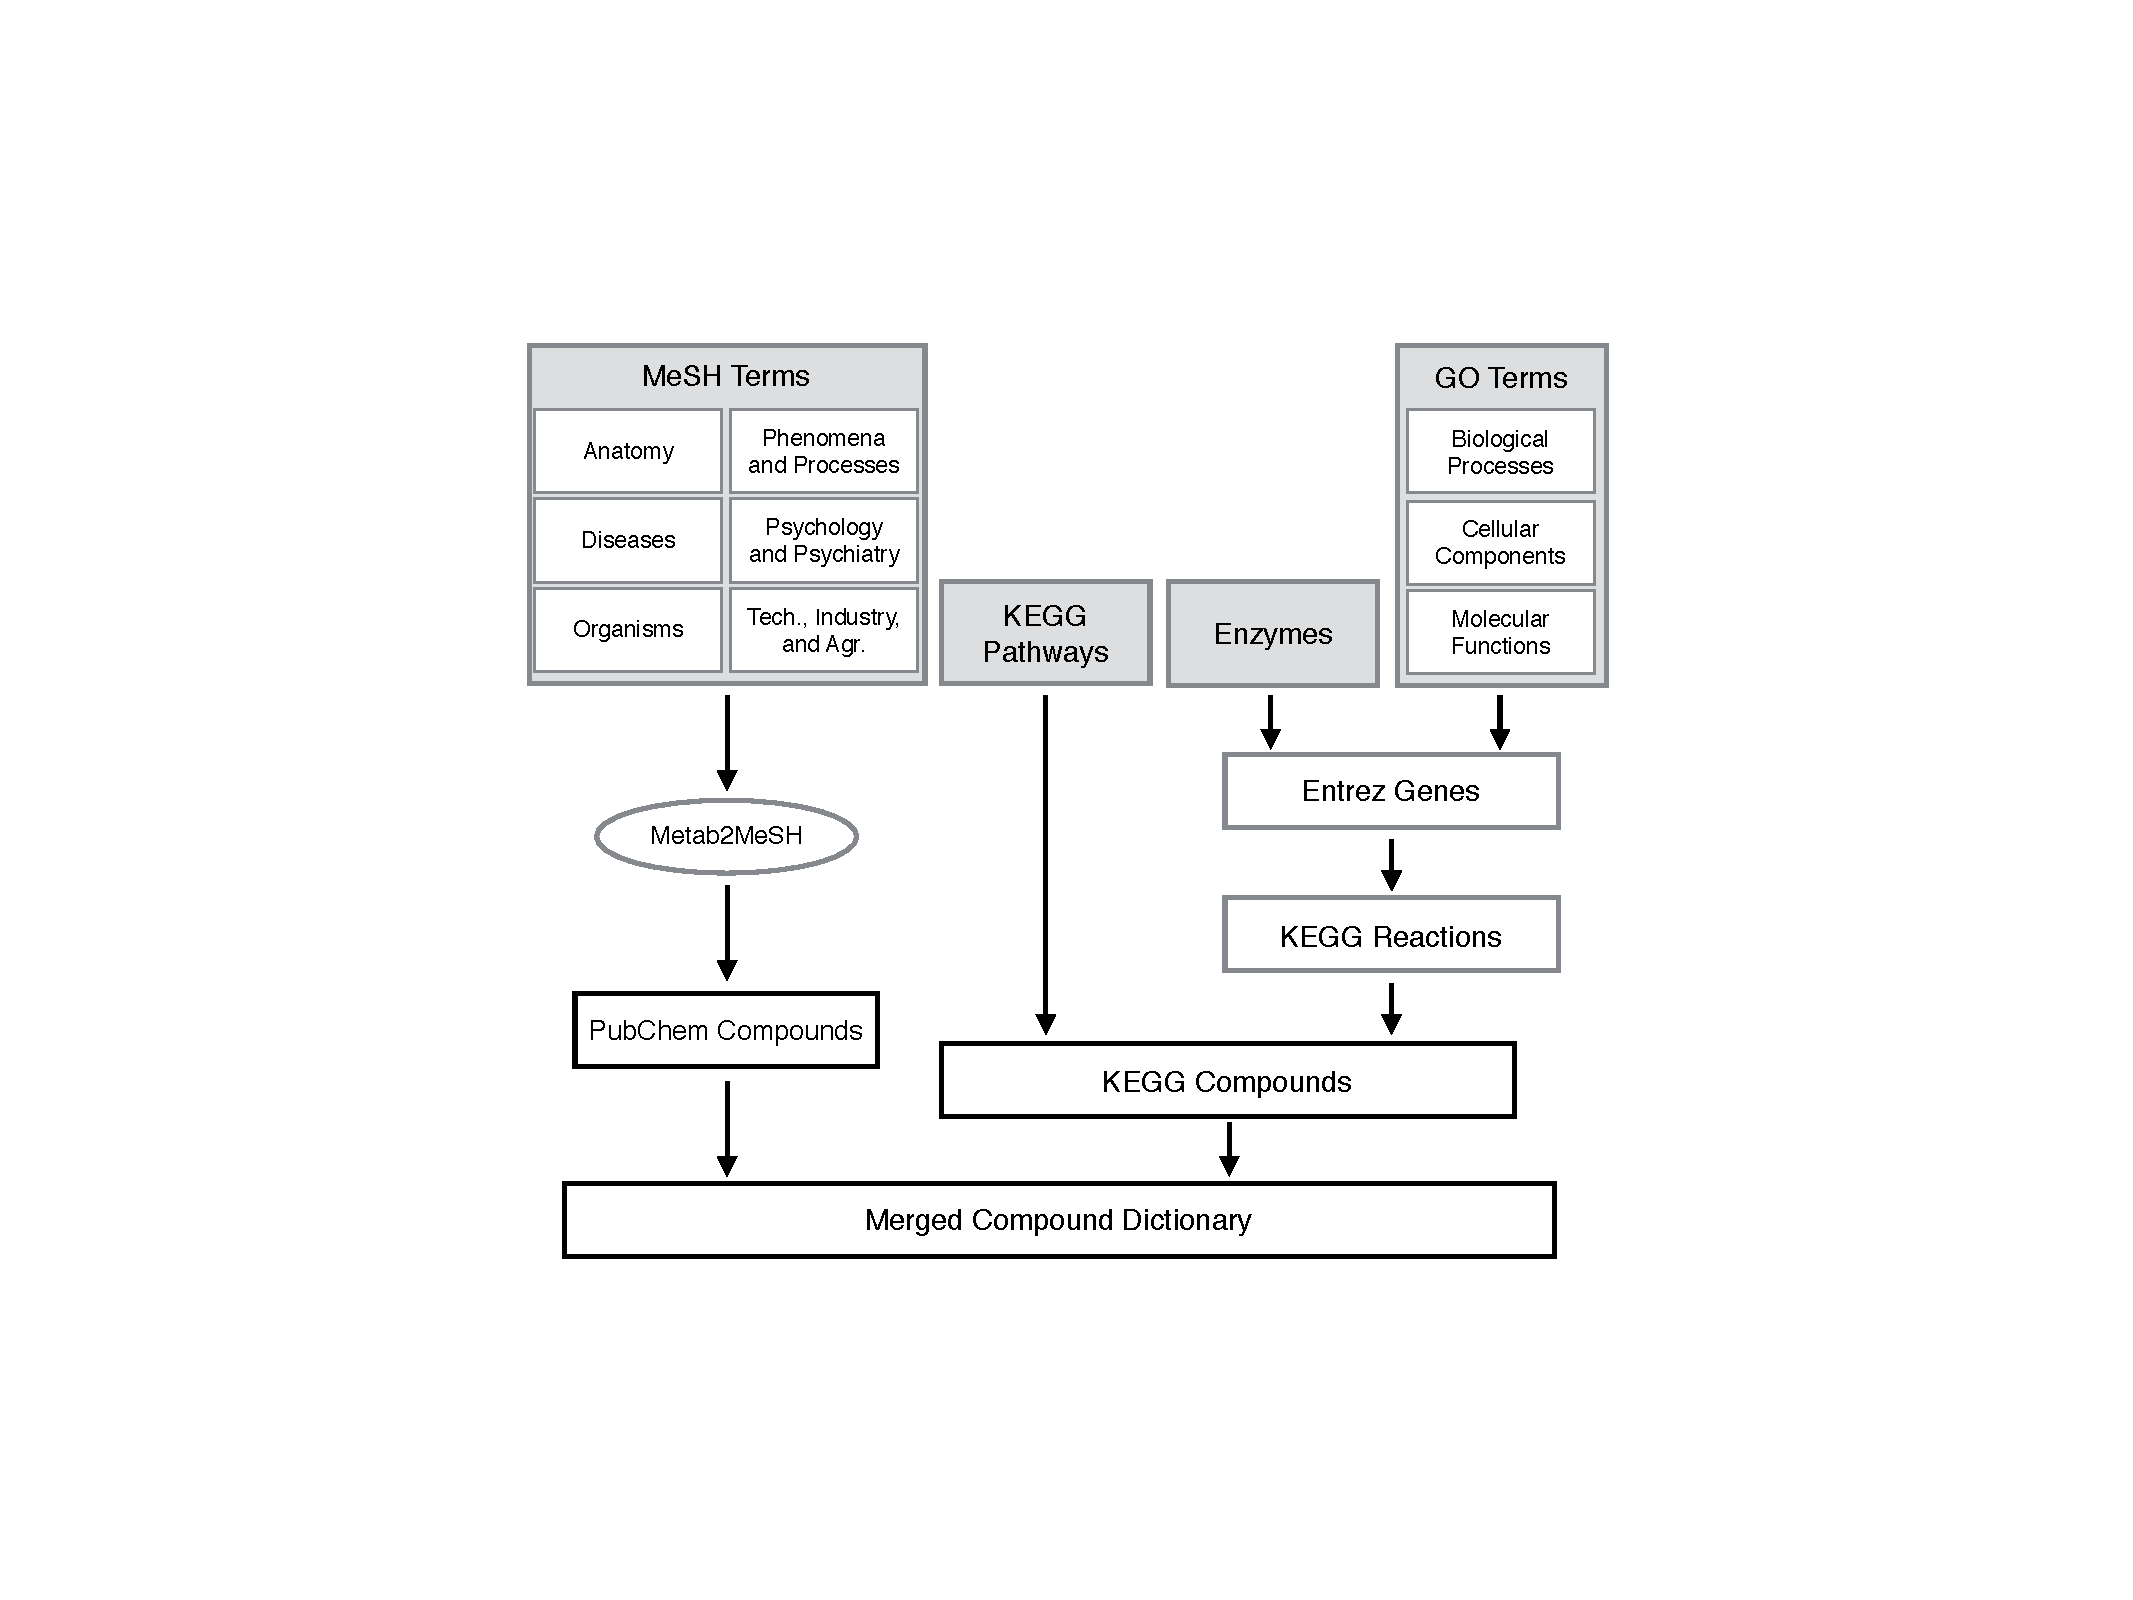
\includegraphics[width=1\textwidth]{chap3figs/figure3_1.pdf}
\caption[A diagrammatic view of how small molecules are annotated to concepts in ConceptMetab.]
{
% Rackham requires the figure list title matches the first sentence, so repeat that sentence here
\textbf{A diagrammatic view of how small molecules are annotated to concepts in ConceptMetab.} PubChem compounds are associated with MeSH Terms via Metab2MeSH. Metabolites with KEGG IDs are associated with KEGG Pathways via their XML representation. Enzymes and GO terms are mapped to KEGG compounds through Entrez genes and KEGG reactions. Finally, PubChem and KEGG small molecules are linked via a dictionary used in Metab2MeSH.
}
\label{chap3:fig:1}
\end{figure}

\newpage

\begin{figure}[ht!]
\centering
% manually adjust the width of the figure
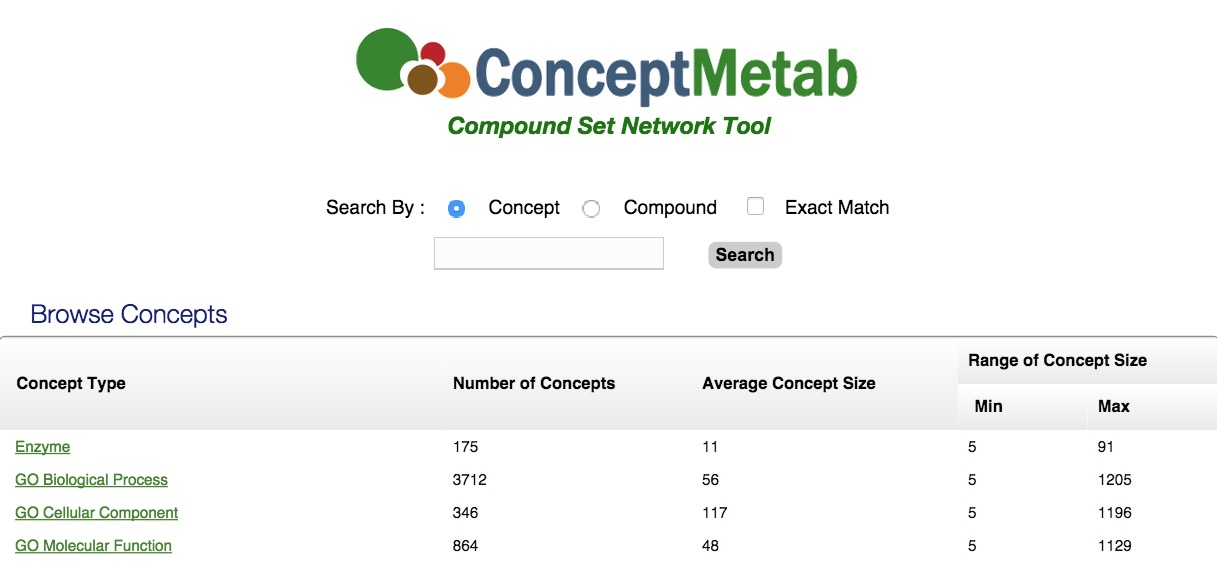
\includegraphics[width=1\textwidth]{chap3figs/figure3_2.jpg}
\caption[Searching in ConceptMetab.]
{
% Rackham requires the figure list title matches the first sentence, so repeat that sentence here
\textbf{Searching in ConceptMetab.} Users may search by biological concept or compound, or browse by concept type.
}
\label{chap3:fig:2}
\end{figure}

\newpage

\begin{figure}[ht!]
\centering
% manually adjust the width of the figure
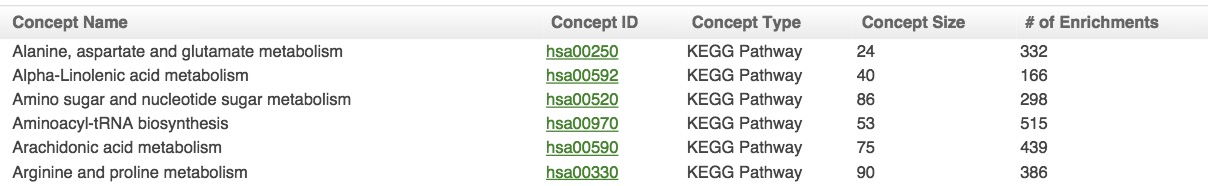
\includegraphics[width=1\textwidth]{chap3figs/figure3_3.jpg}
\caption[Browsing in ConceptMetab.]
{
% Rackham requires the figure list title matches the first sentence, so repeat that sentence here
\textbf{Browsing in ConceptMetab.} Browsing by concept type displays a list of biological concepts, their IDs from the originating database, the number of compounds in each concept, and the number of significantly associated concepts in ConceptMetab ($FDR < 0.05$).
}
\label{chap3:fig:3}
\end{figure}

\newpage

\begin{figure}[ht!]
\centering
% manually adjust the width of the figure
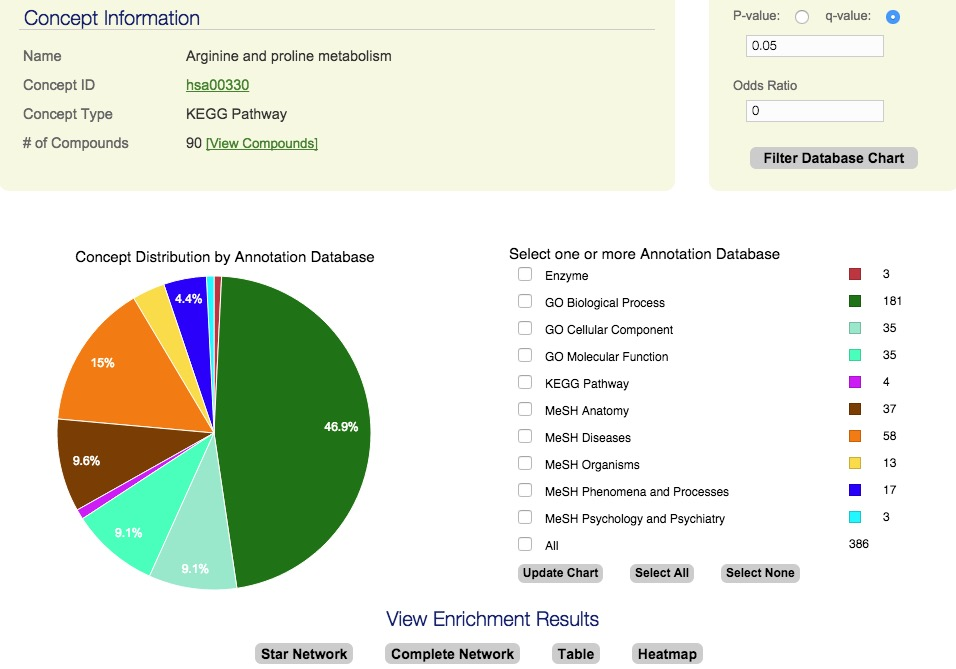
\includegraphics[width=1\textwidth]{chap3figs/figure3_4.jpg}
\caption[Concept overviews.]
{
% Rackham requires the figure list title matches the first sentence, so repeat that sentence here
\textbf{Concept overviews.} Selecting a concept displays an overview, including a summary of the concepts that are significantly associated with the chosen term. Users may alter the criteria for significance. Links are provided to the network visualizations, the enrichment table, and the heatmap.
}
\label{chap3:fig:4}
\end{figure}

\newpage

\begin{figure}[ht!]
\centering
% manually adjust the width of the figure
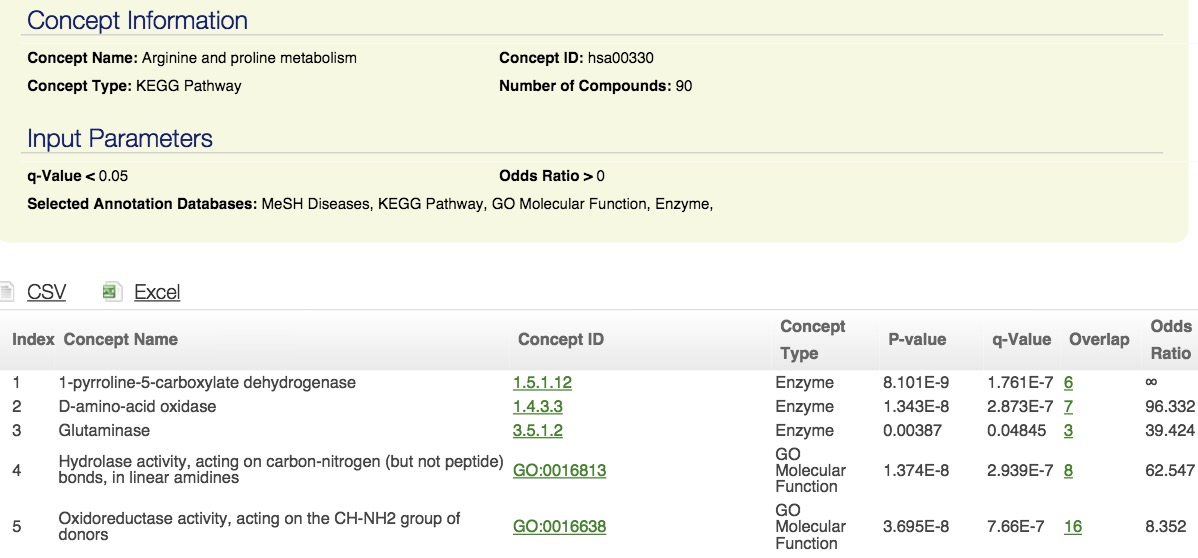
\includegraphics[width=1\textwidth]{chap3figs/figure3_5.jpg}
\caption[Enrichment results.]
{
% Rackham requires the figure list title matches the first sentence, so repeat that sentence here
\textbf{Enrichments results.} The enrichment table displays typical enrichment results with interactive links, and the ability to select individual concepts for inclusion in visualizations.
}
\label{chap3:fig:5}
\end{figure}

\newpage

\begin{figure}[ht!]
\centering
% manually adjust the width of the figure
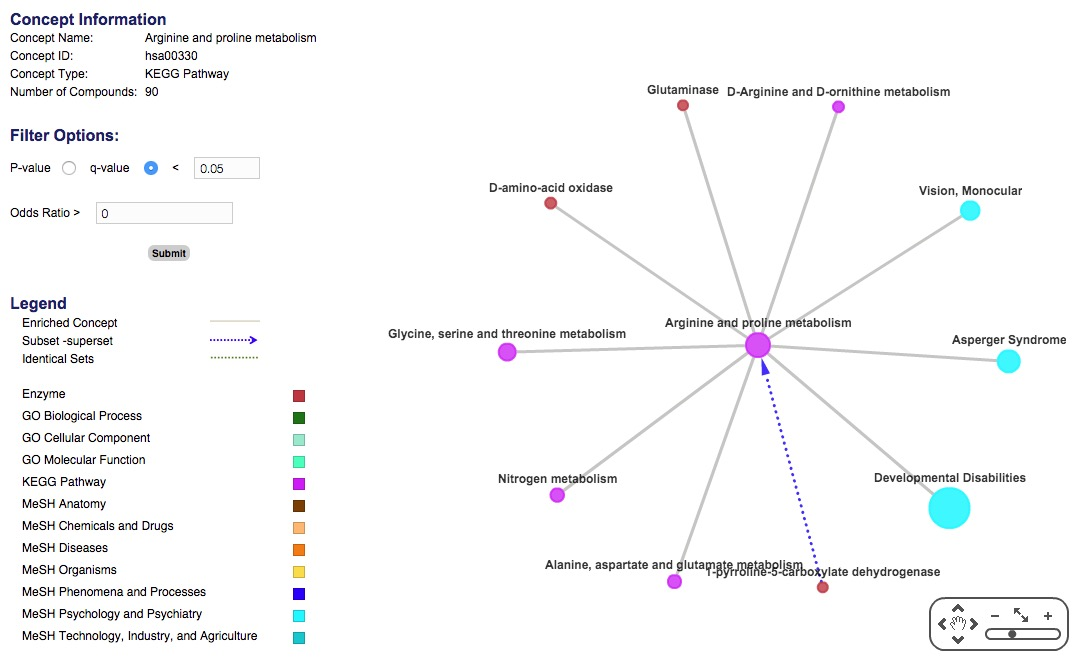
\includegraphics[width=1\textwidth]{chap3figs/figure3_6.jpg}
\caption[Star networks.]
{
% Rackham requires the figure list title matches the first sentence, so repeat that sentence here
\textbf{Star networks.} The star network visualizes concepts significantly associated with the concept. Color represents concept type and the size of node indicates the number of compounds. Clicking on a node displays concept information, and clicking an edge displays the compounds in common between the two concepts.
}
\label{chap3:fig:6}
\end{figure}

\newpage

\begin{figure}[ht!]
\centering
% manually adjust the width of the figure
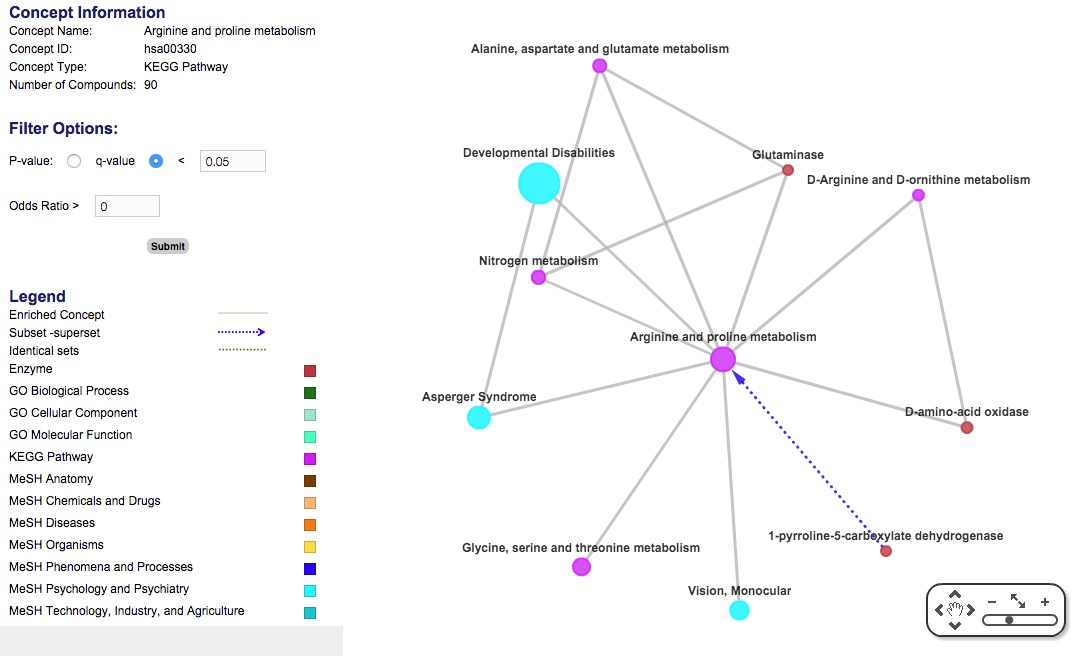
\includegraphics[width=1\textwidth]{chap3figs/figure3_7.jpg}
\caption[Complete networks.]
{
% Rackham requires the figure list title matches the first sentence, so repeat that sentence here
\textbf{Complete networks.} The complete network contains the same nodes as the star network, but also displays associations among the nodes.
}
\label{chap3:fig:7}
\end{figure}

\newpage

\begin{figure}[ht!]
\centering
% manually adjust the width of the figure
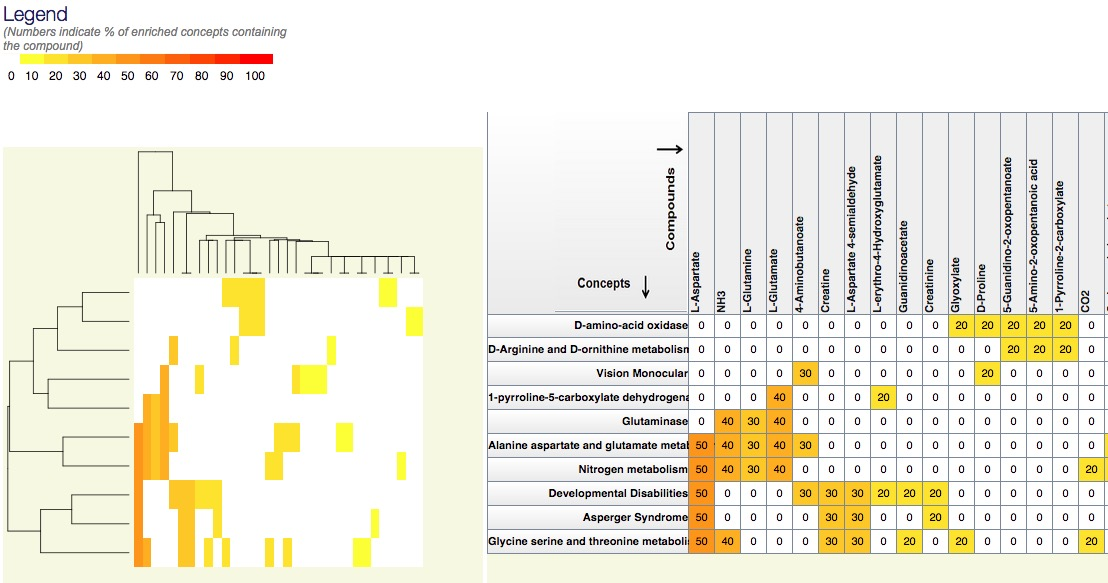
\includegraphics[width=1\textwidth]{chap3figs/figure3_8.jpg}
\caption[Heatmap.]
{
% Rackham requires the figure list title matches the first sentence, so repeat that sentence here
\textbf{Heatmap.} The heatmap allows users to investigate the compounds that are responsible for the observed associations. An overview heatmap image and an interactive version are provided.
}
\label{chap3:fig:8}
\end{figure}

\newpage

\begin{figure}[ht!]
\centering
% manually adjust the width of the figure
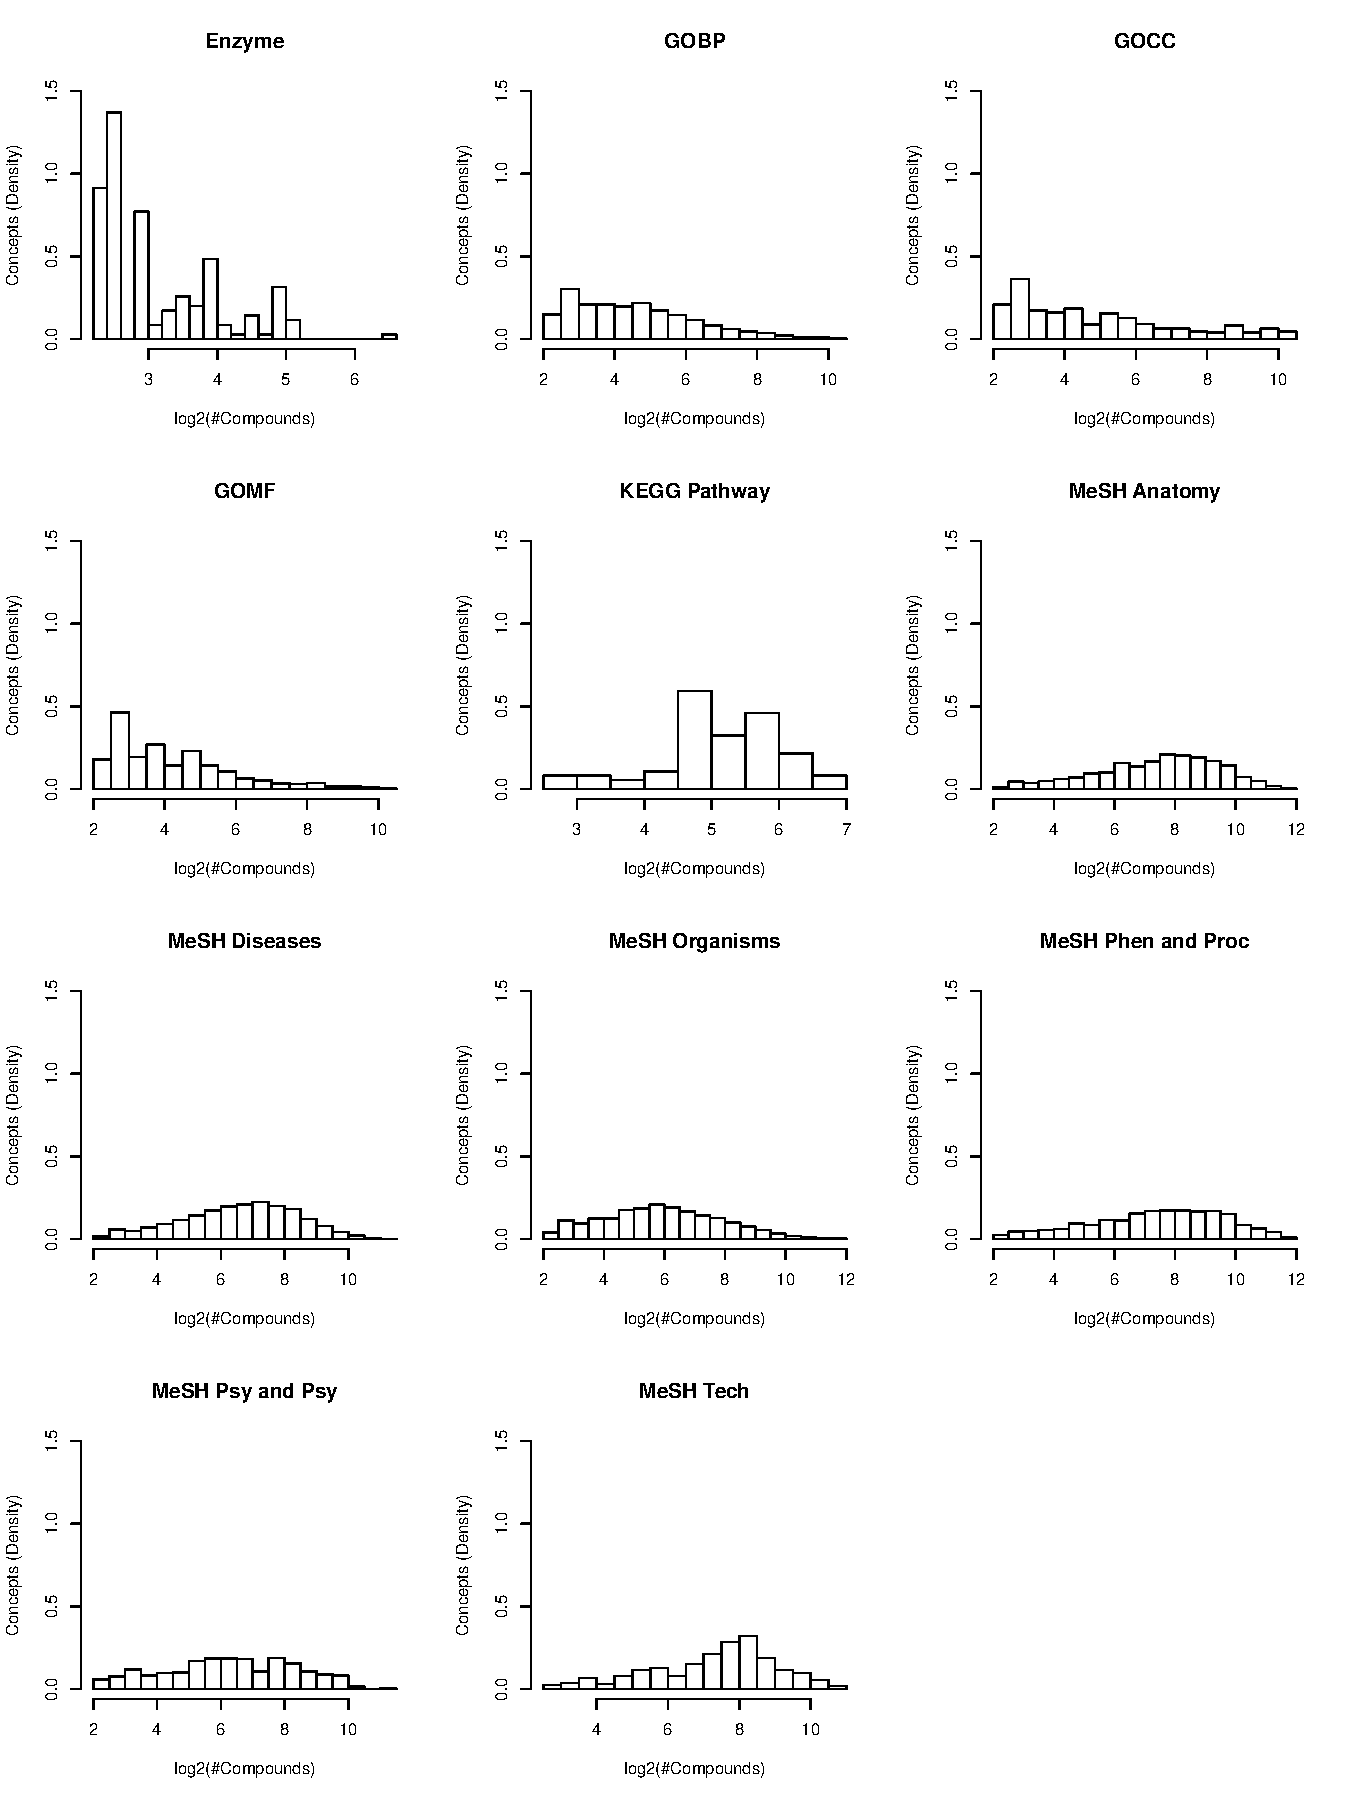
\includegraphics[width=1\textwidth]{chap3figs/figure3_10.pdf}
\caption[Distributions of the number of compounds per concept for each concept type.]
{
% Rackham requires the figure list title matches the first sentence, so repeat that sentence here
\textbf{Distributions of the number of compounds per concept for each concept type.} GOBP=Gene Ontology (GO) biological process; GOCC=GO cellular component; GOMF=GO molecular function.

}
\label{chap3:fig:9}
\end{figure}

\newpage

\begin{figure}[ht!]
\centering
% manually adjust the width of the figure
\includegraphics[width=1\textwidth]{chap3figs/figure3_9.pdf}
\caption[Distributions of the number of concepts per compound for each concept type.]
{
% Rackham requires the figure list title matches the first sentence, so repeat that sentence here
\textbf{Distributions of the number of concepts per compound for each concept type.}

}
\label{chap3:fig:10}
\end{figure}

\newpage

\begin{figure}[ht!]
\centering
% manually adjust the width of the figure
\includegraphics[width=1\textwidth]{chap3figs/figure3_11.pdf}
\caption[Proportion of enrichments between concept types.]
{
% Rackham requires the figure list title matches the first sentence, so repeat that sentence here
\textbf{Percentage of enrichments between concept types.} Numbers in each cell are the percentage of enrichment tests between the respective concept types which were significant ($FDR < 0.05$). Observe that KEGG-based concepts tend to be more enriched with other KEGG-based concepts, and similarly for PubChem-based concepts.
}
\label{chap3:fig:11}
\end{figure}

\newpage

\begin{figure}[ht!]
\centering
% manually adjust the width of the figure
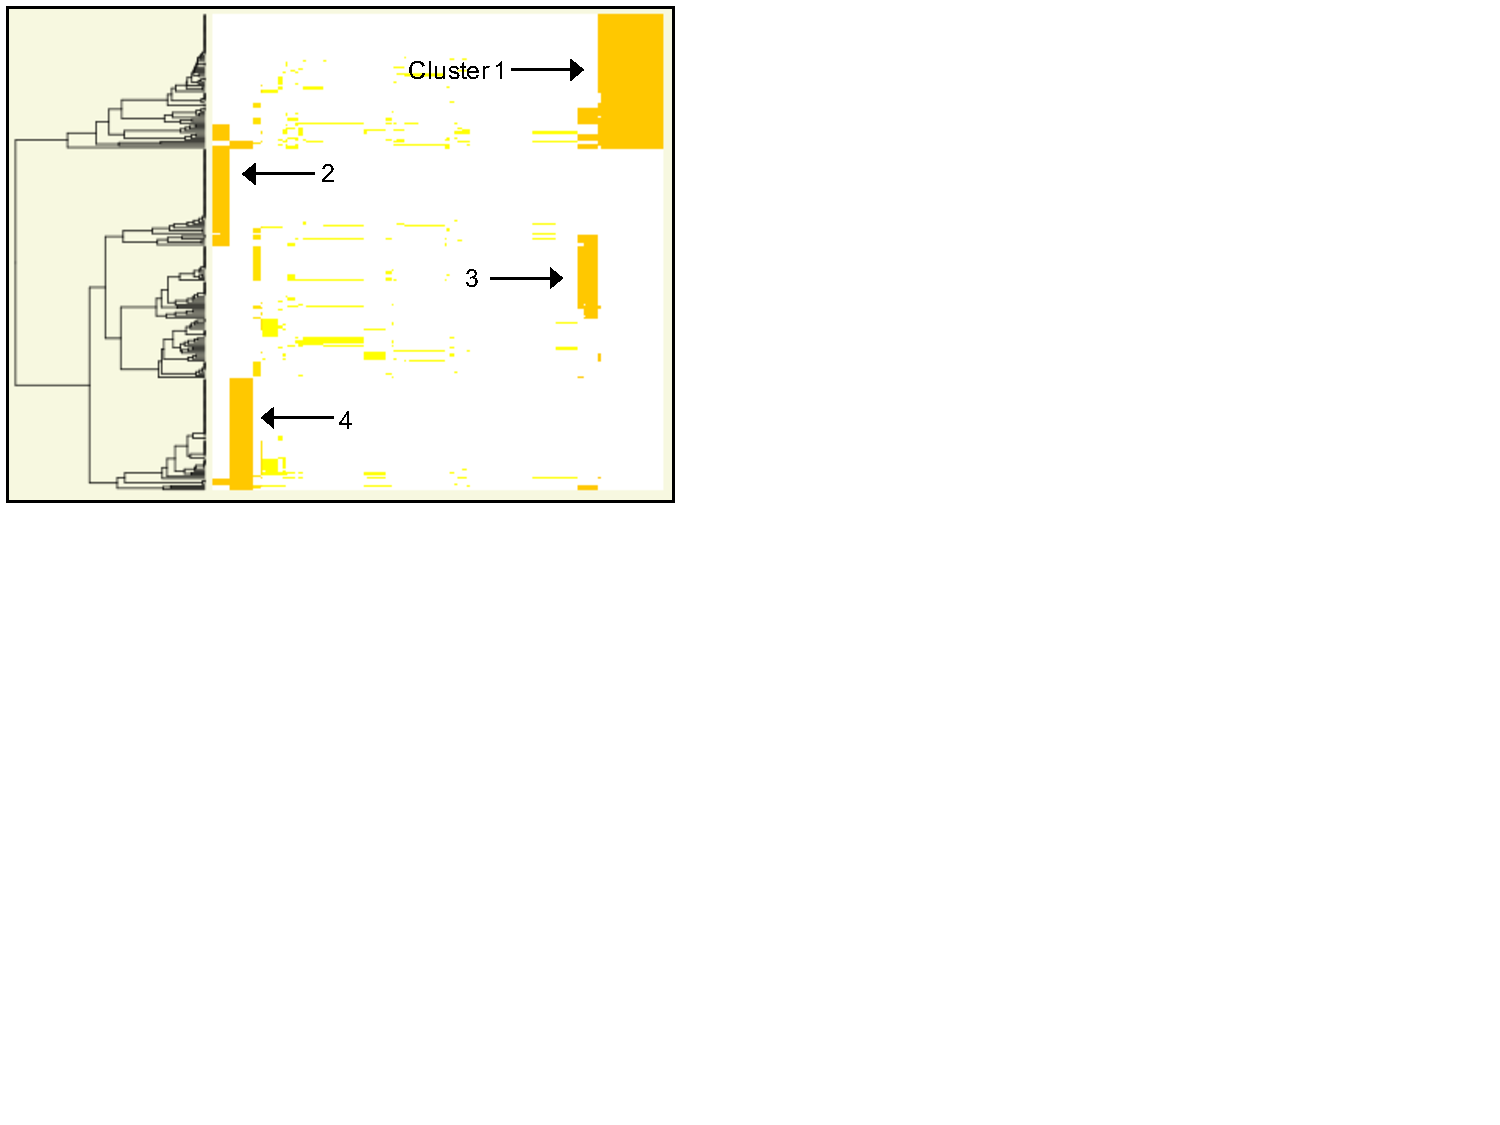
\includegraphics[width=1\textwidth]{chap3figs/figure3_12.pdf}
\caption[Overview heatmap for diseases associated with Unfolded Protein Response.]
{
% Rackham requires the figure list title matches the first sentence, so repeat that sentence here
\textbf{Overview heatmap for diseases associated with Unfolded Protein Response.} Each row represents a MeSH disease and each column is a compound. The UPR is associated with four main groups of diseases, defined by the types of overlapping compounds.  From here, users may click to proceed to an interactive heatmap view.
}
\label{chap3:fig:12}
\end{figure}

\newpage

\begin{figure}[ht!]
\centering
% manually adjust the width of the figure
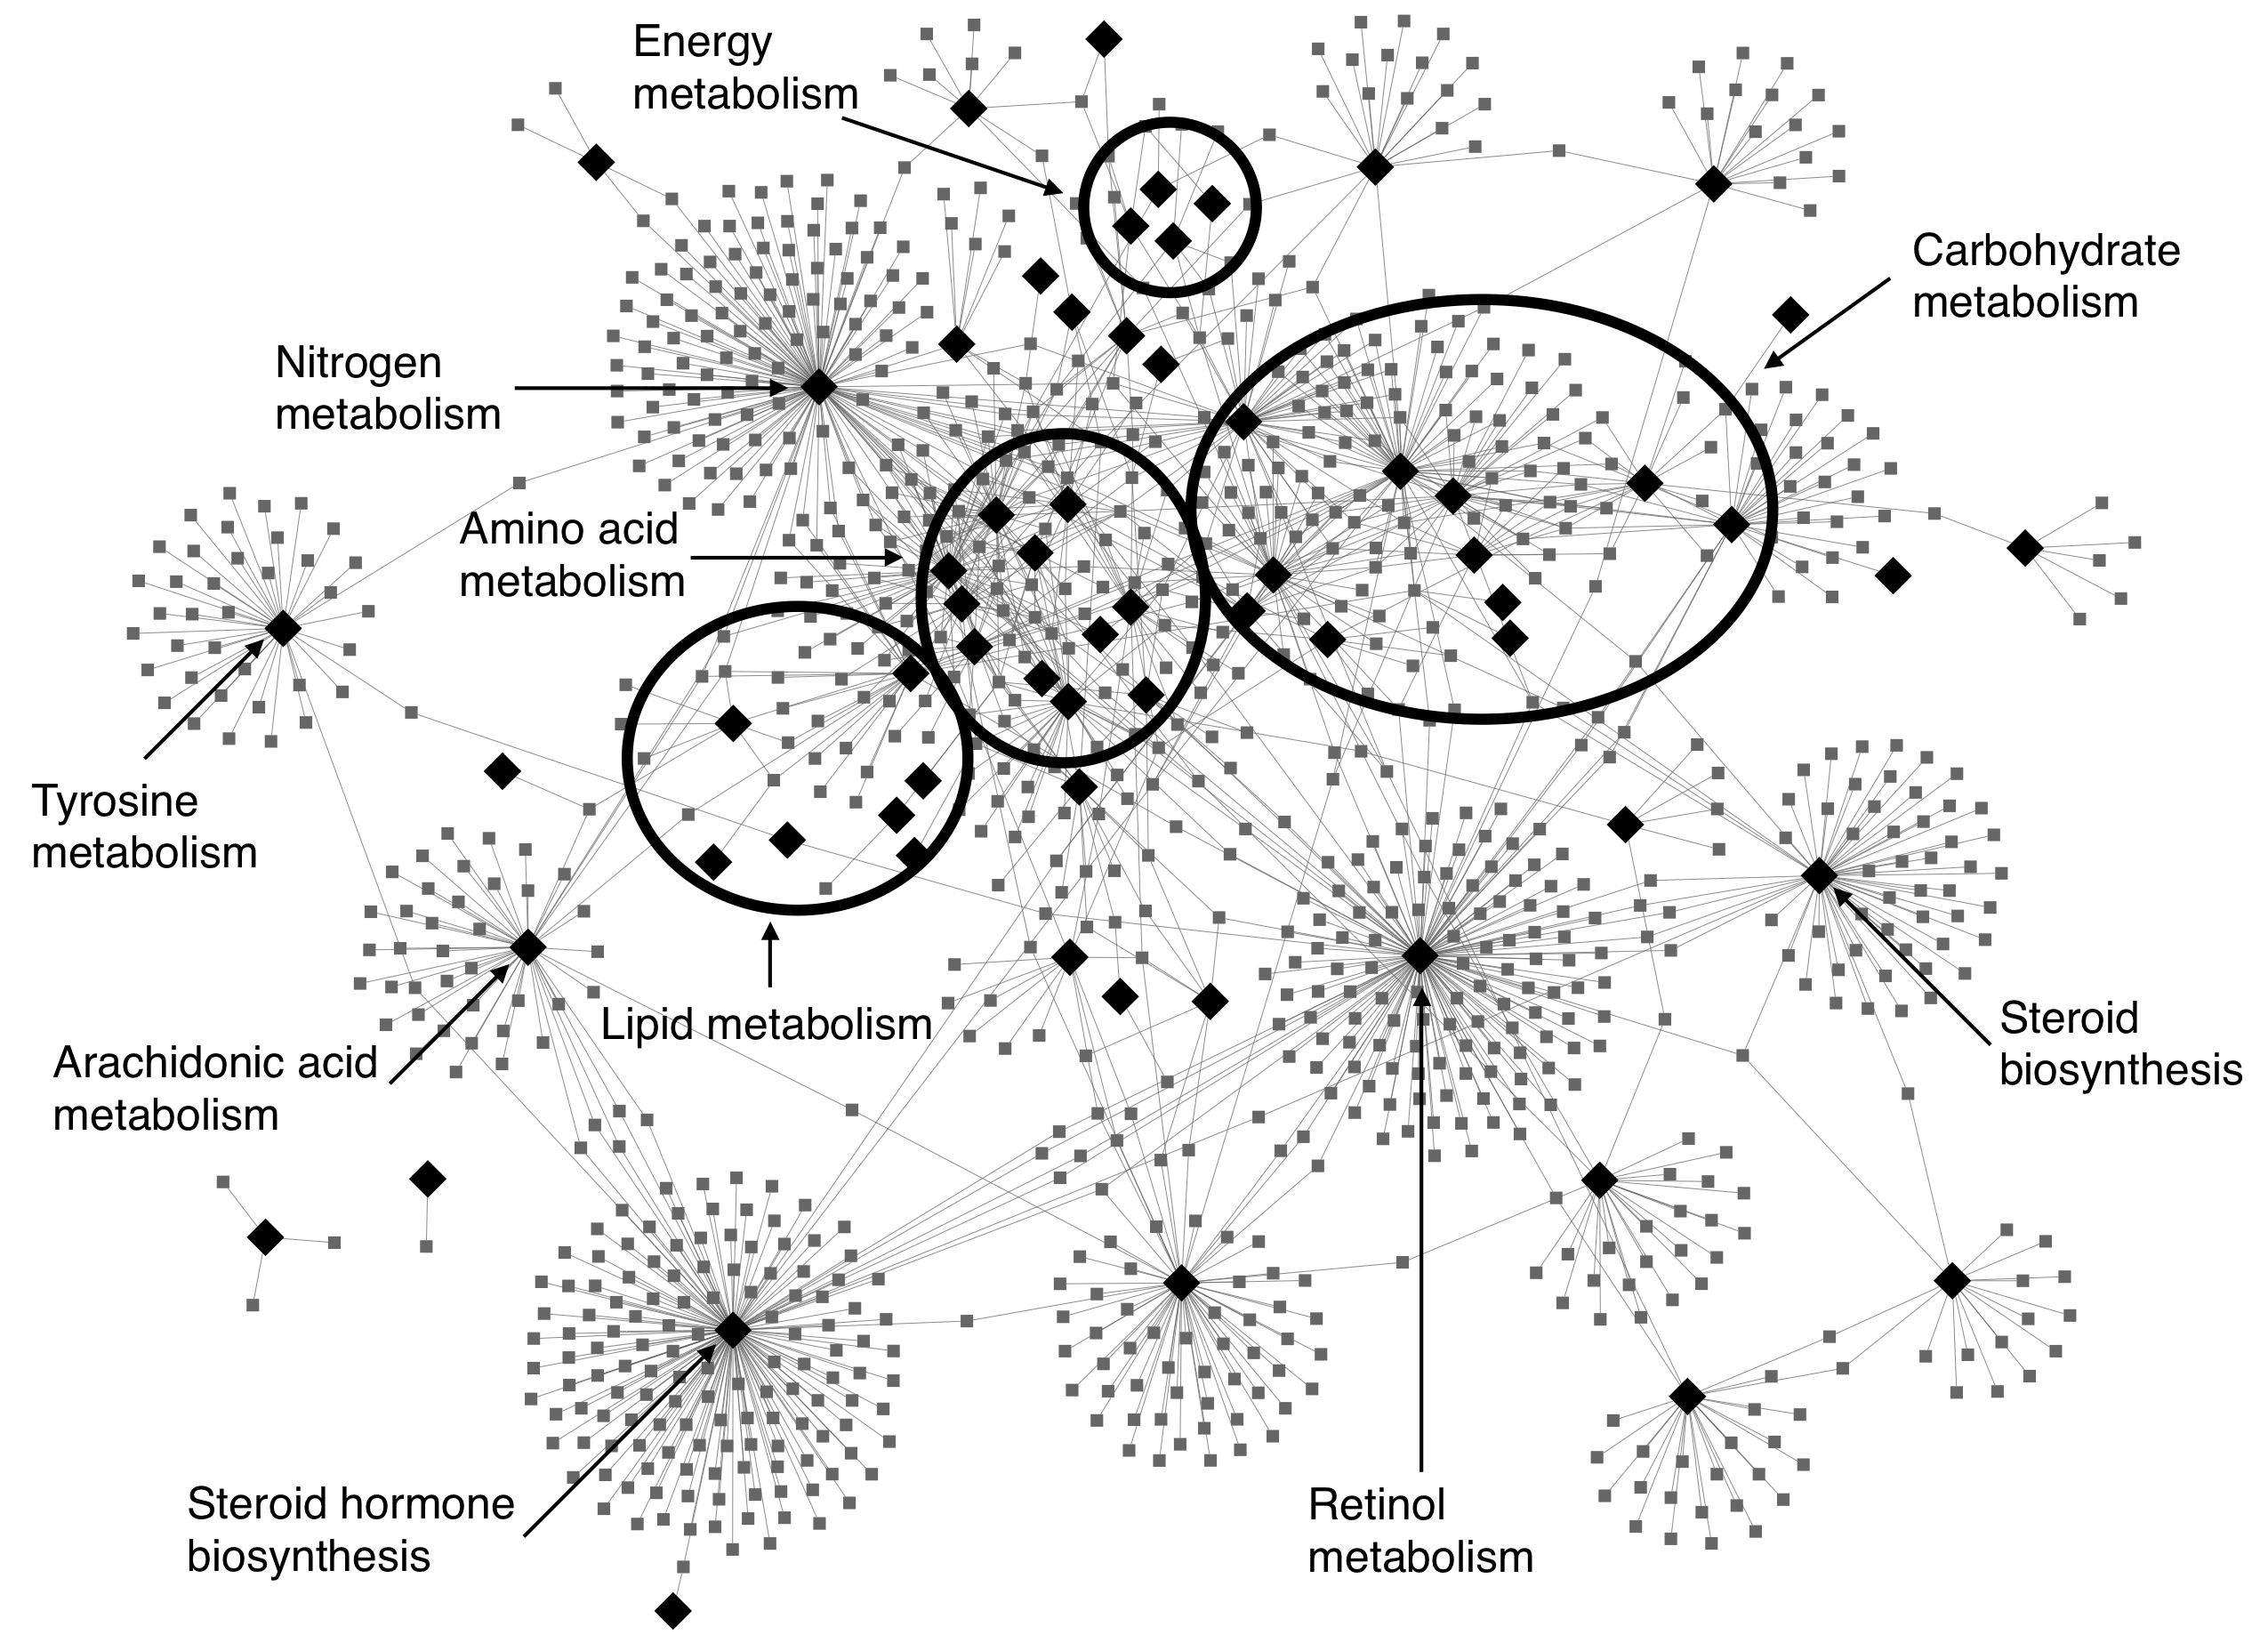
\includegraphics[width=1\textwidth]{chap3figs/figure3_13.jpg}
\caption[Bipartite metabolic pathway.]
{
% Rackham requires the figure list title matches the first sentence, so repeat that sentence here
\textbf{Bipartite metabolic pathway.} A disease network identified by ConceptMetab and displayed in Cytoscape. Black diamonds represent pathways; grey squares are diseases. The ovals in the center represent groups of several KEGG pathways, e.g. carbohydrate metabolism includes amino sugar, nucleotide sugar, galactose, fructose and mannose metabolism.

}
\label{chap3:fig:13}
\end{figure}

\newpage

\begin{figure}[ht!]
\centering
% manually adjust the width of the figure
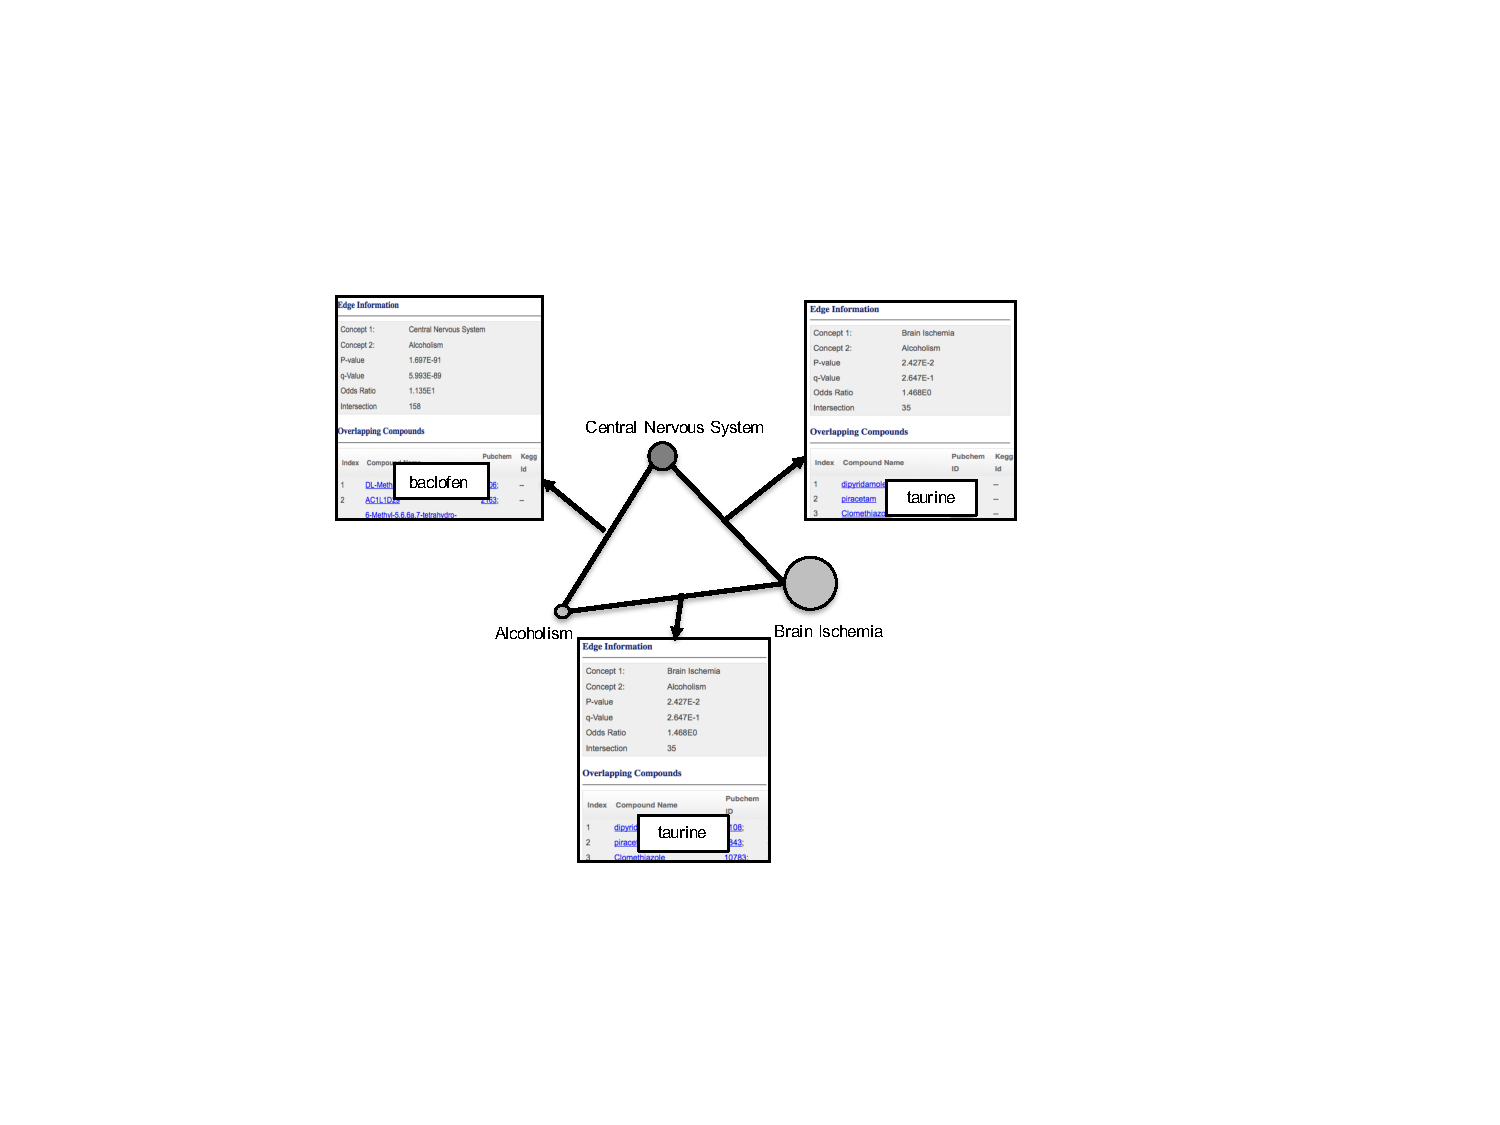
\includegraphics[width=1\textwidth]{chap3figs/figure3_14.pdf}
\caption[ConceptMetab complete network.]
{
% Rackham requires the figure list title matches the first sentence, so repeat that sentence here
\textbf{ConceptMetab complete network.} Network nodes represent concepts. By clicking on an edge user can obtain the information about compounds that are in common between concepts.

}
\label{chap3:fig:14}
\end{figure}

\clearpage
\section*{Tables}
\begin{table}[!ht]
\small
\centering
\begin{tabular}{l|llll}
\textbf{Concept Type}       & \textbf{\# Concepts} & \textbf{Mean Size} & \textbf{Median Size} & \textbf{\# Compounds} \\\hline
\textbf{Enzyme}             & 175                  & 11                 & 7                    & 874                   \\
\textbf{GOBP}               & 3712                 & 56                 & 20                   & 1220                  \\
\textbf{GOCC}               & 346                  & 117                & 19                   & 1213                  \\
\textbf{GOMF}               & 864                  & 48                 & 14                   & 1226                  \\
\textbf{KEGG Pathway}       & 74                   & 42                 & 38                   & 2427                  \\
\textbf{MeSH Anatomy}       & 1506                 & 357                & 208                  & 37706                 \\
\textbf{MeSH Diseases}      & 4089                 & 182                & 105                  & 33074                 \\
\textbf{MeSH Organisms}     & 3011                 & 150                & 58                   & 48688                 \\
\textbf{MeSH Phen and Proc} & 1443                 & 404                & 195                  & 43016                 \\
\textbf{MeSH Psy and Psy}   & 519                  & 180                & 79                   & 9188                  \\
\textbf{MeSH Tech}          & 330                  & 280                & 198                  & 15721
\end{tabular}
\normalsize
\caption[An overview of the annotation databases in ConceptMetab.]
{
% Rackham requires the figure list title matches the first sentence, so repeat that sentence here
\textbf{An overview of the annotation databases in ConceptMetab.}
The number of biological concepts, the mean and median number of compounds in them, and the number of unique compounds across all concepts in each concept type are given.
}
\label{chap3:table:1}

\end{table}

\newpage

\begin{sidewaystable}[!ht]
\tiny
\centering
\begin{tabular}{l|p{1.5cm}p{1.5cm}|p{1cm}p{1cm}p{1cm}p{1cm}|p{2cm}p{2cm}p{2cm}|p{2cm}}
\textbf{}             & \multicolumn{2}{l}{\textbf{Query Methods}}                        & \multicolumn{4}{l}{\textbf{Annotations}}                                     & \multicolumn{3}{l}{\textbf{Enrichment and Mapping}}                                                                                                         & \textbf{Visualizations} \\
\textbf{Tool}         & \textbf{Query by Biological Concept} & \textbf{Query by Compound} & \textbf{MeSH} & \textbf{Metabolic Pathways} & \textbf{GO} & \textbf{Enzymes} & \textbf{Pathway Mapping of User-supplied Compounds} & \textbf{Enrichment of User-supplied Compound Sets} & \textbf{Enrichment of Pre-defined Compound Sets} & \textbf{}               \\\hline
\textbf{ConceptMetab} & Yes                                  & Yes                        & Yes           & Yes                         & Yes         & Yes              & No                                                  & No                                                 & Yes                                              & Yes                     \\
\textbf{MetScape}     & No                                   & Yes                        & Yes           & Yes                         & No          & Yes              & Yes                                                 & No                                                 & No                                               & Yes                     \\
\textbf{MetDisease}   & No                                   & Yes                        & Yes           & Yes                         & No          & Yes              & No                                                  & No                                                 & No                                               & Yes                     \\
\textbf{Metab2MeSH}   & No                                   & Yes                        & Yes           & No                          & No          & No               & No                                                  & No                                                 & No                                               & No                      \\
\textbf{MBRole}       & No                                   & No                         & No            & Yes                         & No          & Yes              & Yes                                                 & Yes                                                & No                                               & No                      \\
\textbf{MSEA}         & No                                   & No                         & No            & Yes                         & No          & Yes              & Yes                                                 & Yes                                                & No                                               & Yes                     \\
\textbf{MetPA}        & No                                   & No                         & No            & Yes                         & No          & Yes              & Yes                                                 & Yes                                                & No                                               & Yes
\end{tabular}
\normalsize
\caption[A feature comparison of ConceptMetab and other metabolite-related tools.]
{
% Rackham requires the figure list title matches the first sentence, so repeat that sentence here
\textbf{A feature comparison of ConceptMetab and other metabolite-related tools.}
}
\label{chap3:table:2}

\end{sidewaystable}


\chapter{annotatr: Genomic regions in context}
\label{chap4}
\noindent This work has been published as: \textbf{R. G. Cavalcante} and M. A. Sartor, "annotatr: Genomic regions in context.," \emph{Bioinformatics}, Mar. 2017.

%%%%%%%%%%%%%%%%%%%%%%%%%%%%%%%%%%%%%%%%%%%%%%%%%%%%%%%%%%%%%%%%%%%%%%%%%%%%%%%%
\section{Introduction}
\label{annotatr_introduction}

Genomic regions resulting from next-generation sequencing experiments and bioinformatics pipelines require annotation to genomic features for context. For example, hyper-methylation of CpG shores in promoters may indicate different regulatory regimes in one condition compared to another, or it may be of interest that a transcription factor overwhelmingly binds in enhancers, while another tends to bind at exon-intron boundaries.

While tools exist to intersect genomic regions of interest with genomic annotations, we found the annotations, methods of intersection, and graphics options had room for improvement. ChIPpeakAnno \cite{Zhu:2010be} is an R package that has been used in many studies across a variety of organisms. It returns only one genomic annotation per input region, and while providing the user with some plots, these are limited by their inability to incorporate data associated with the regions of interest such as methylation rates, fold changes, etc. Another R package, goldmine \cite{Bhasin:2016bk}, returns either all annotations intersecting regions of interest (a one-to-many mapping) or annotations based on a prioritization (a one-to-one mapping). The goldmine package provides helper functions to create annotations from any UCSC genome browser table. However, it does not offer built-in functions for summary plots, nor to plot data related to the regions over the annotations. Outside of the R ecosystem, BEDtools \cite{Quinlan:2010km}, implemented in C++, intersects and aggregates genomic regions with annotations, and is very fast. However, its more general purpose means users must provide all annotations and manually generate plots.

We developed annotatr, a Bioconductor package that reports all intersections of genomic regions with built-in genomic annotations for D. melanogaster (dm3 and dm6), H. Sapiens (hg19 and hg38), M. musculus (mm9 and mm10), R. norvegicus (rn4, rn5, and rn6), annotations imported from the AnnotationHub R package, or custom annotations for any organism. annotatr enables users to associate numerical or categorical data with regions, enabling better understanding of the underlying experiments via summarization and visualization functions. annotatr is fast, flexible, and easily included in bioinformatics pipelines.

%%%%%%%%%%%%%%%%%%%%%%%%%%%%%%%%%%%%%%%%%%%%%%%%%%%%%%%%%%%%%%%%%%%%%%%%%%%%%%%%
\section{Methods}
\label{annotatr_methods}

%%%%%%%%%%%%%%%%%%%%%%%%%%%%%%%%%%%%%%
\subsection{Construction of genomic annotations}
\label{annotatr_methods_construction}

%%%%%%%%%%%%%%%%%%%
\subsubsection{CpG features}
We use the AnnotationHub R package (Morgan, 2016) to obtain the CpG island annotations when available (hg19, mm9, rn4, and rn5), and otherwise use the UCSC Golden Path (hg38, mm10, and rn6). Using functions in the GenomicRanges R package \cite{Lawrence:2013hi}, we defined CpG shores as 2kb upstream and downstream of the CpG island boundaries and excluding CpG islands. CpG shelves are defined as the 2kb regions immediately upstream and downstream of the CpG shores opposite of the CpG island. Again, this excludes regions already annotated as CpG islands and CpG shores. See Figure \ref{chap4:fig:1} for a schematic of the CpG annotations, and Table \ref{chap4:table:1} for the organisms and genome builds with CpG annotations.

%%%%%%%%%%%%%%%%%%%
\subsubsection{Genic features}
We use the TxDb R packages for the specified genomes (e.g. the Bioconductor package: TxDb.Hsapiens.UCSC.hg19.knownGene (Carlson, 2015) for human genome version hg19) and functions from the GenomicFeatures R package \cite{Lawrence:2013hi} to extract 1-5kb regions upstream of a TSS, promoters ($<$1Kb upstream of a TSS), 5'UTRs, exons, introns, and 3'UTRs. Intron/exon and exon/intron boundaries are defined as 200bp around the boundary. Intergenic annotations are taken to be the complement of the aforementioned annotations. We allow all genic annotations to overlap. See Figure \ref{chap4:fig:1} for a schematic of the genic annotations, and Table \ref{chap4:table:1} for organisms and genome builds with genic annotations.

%%%%%%%%%%%%%%%%%%%
\subsubsection{lncRNA features}
We use GENCODE long non-coding RNAs (lncRNA) from GENCODE at the transcript level \cite{Harrow:2012cx}. For hg19 we use GENCODE v19, for hg38 we use GENCODE v23, and for mm10 we use GENCODE vM6. Relevant GENCODE biotypes (\url{https://www.gencodegenes.org/gencode_biotypes.html}) are included as part of the annotations.

%%%%%%%%%%%%%%%%%%%
\subsubsection{Enhancer features}
We use enhancers defined via bi-directional CAGE transcription from the FANTOM5 consortium \cite{Andersson:2014bn} for human (hg19) and mouse (mm9). We provide enhancer annotations for hg38 and mm10 with the rtracklayer::liftover() function on the hg19 and mm9 enhancer annotations. Additional enhancer regions are defined within the chromatin state features (see below). Enhancers in hg38 and mm10 will be available in the April 2017 Bioconductor release, or users may download annotatr from the GitHub repository to use this feature.

%%%%%%%%%%%%%%%%%%%
\subsubsection{Chromatin state features}
We use the chromatin states given by chromHMM \cite{Ernst:2012ii} in each of 9 human cell lines. The cell lines are: GM12878, H1-hESC, HepG2, HUVEC, HMEC, HSMM, K562, NHEK, NHLF. The genomic coordinates are with respect to hg19 only. In brief, numerous ChIP-seq experiments and a hidden Markov model were used to segment the genome into the following 15 functional chromatin states: active promoter, weak promoter, inactive/poised promoter, strong enhancer (2 classes), weak enhancer (2 classes), insulator, transcriptional transition, transcriptional elongation, weak transcribed, polycomb repressed, heterochromatin, and repetitive/CNV (2 classes).

%%%%%%%%%%%%%%%%%%%
\subsubsection{AnnotationHub resources}
Any GRanges class resource from the AnnotationHub R package can be converted to an annotatr annotation via the build\_ah\_annots() function. Some resources of special interest to users may be COSMIC mutations, GWAS catalog mutations, and ENCODE/Roadmap Epigenomics datasets. Among the ENCODE and Roadmap datasets are many transcription factor binding peaks and histone modification peaks. This feature will be available in the April 2017 Bioconductor release, or users may download annotatr from the GitHub repository to use this feature.

%%%%%%%%%%%%%%%%%%%%%%%%%%%%%%%%%%%%%%
\subsection{Benchmarking with microbenchmark and lineprof}
\label{annotatr_methods_benchmarking}

The microbenchmark R package (Mersmann, 2015) was used on three data sets to compare runtimes over 10 runs of annotatr v1.0.1, ChIPpeakAnno v3.8.1 \cite{Zhu:2010be}, and goldmine v1.0.0 \cite{Bhasin:2016bk}.

Benchmarks were run on our lab server containing 40 cores and 128 GB of RAM. The three data sets, ranging in size from 31,000 to 2,500,000 lines, are:

\begin{enumerate}
	\item A ~31,000 line ChIP-seq peak file from ENCODE for Pol2 in the Gm12878 cell line \cite{ENCODEProjectConsortium:2012gc}.
	\item A ~290,000 line file of hydroxymethylation peaks resulting from macs2 \cite{Zhang:2008gm} on GEO dataset GSE52945 \cite{Figueroa:2010ch}.
	\item A ~2,500,000 line CpG bedGraph report from Bismark \cite{Krueger:2011eb} on a whole genome bisulfite sequencing run (unpublished data).
\end{enumerate}

%%%%%%%%%%%%%%%%%%%%%%%%%%%%%%%%%%%%%%%%%%%%%%%%%%%%%%%%%%%%%%%%%%%%%%%%%%%%%%%%
\section{Results}
\label{annotatr_results}

%%%%%%%%%%%%%%%%%%%%%%%%%%%%%%%%%%%%%%
\subsection{Implementation and features}
\label{annotatr_results_implementation}

A core feature of annotatr is the variety of standard and specialized genomic annotations it includes. Standard annotations include CpG island related features (CpG islands, shores, shelves, and "open sea") and genic features (promoters, 5'UTRs, exons, introns, CDS, and 3'UTRs) (Figure \ref{chap4:fig:1}). Specialized genomic annotations include intron/exon boundaries, enhancers, lncRNAs, and chromatin state segmentations. A built-in function easily transforms resources in the AnnotationHub R package (such as COSMIC, ENCODE, and Roadmap Epigenomics) into usable annotations. Finally, custom annotations can supplement built-in annotations or enable annotation to any organism.

The annotatr package consists of four modules that read, annotate, summarize, and visualize genomic regions. The read module reads a BED6+ file, defined as BED6 and any number of numerical or categorical data columns (Table \ref{chap4:table:2}). The annotate module reports the overlap of all input regions with all intersecting genomic annotations selected by the user, with a user-defined threshold overlap between regions and annotations (Figure \ref{chap4:table:3}). The summarize module enables users to quickly compute summarized information of any numerical (Table \ref{chap4:table:4}) or categorical data (Table \ref{chap4:table:4}) over the annotations.

The collective goal of the visualization module is to provide insight into modes of regulation, and to discover specific relationships among the input regions and genomic annotations with minimum code or forethought. Consider bisulfite sequencing results from methylSig \cite{Park:2014ho} reporting genome-wide differential methylation (DM) between two sample groups. It has columns for DM status (hyper, hypo, none), p-value, methylation difference between the groups, and methylation rates of each group. The annotatr package implements functions to show: 1) the number of DM regions in each annotation type with the option to compare against randomized regions (Figure \ref{chap4:fig:2}), 2) a heatmap of the number of regions annotated to pairs of annotation types (Figure \ref{chap4:fig:3}), 3) the distribution of numerical data across the annotations or any categorical variable (Figure \ref{chap4:fig:4}), 4) the joint distribution of two numerical data columns across the annotations or any categorical variable (Figure \ref{chap4:fig:5}), 5) the distribution of numerical data for regions in any two intersecting annotations (Figure \ref{chap4:fig:6}), and 6) the distribution of a categorical variable across the annotations or any other categorical variable (Figure \ref{chap4:fig:7}).

%%%%%%%%%%%%%%%%%%%%%%%%%%%%%%%%%%%%%%
\subsection{Benchmarking}
\label{annotatr_results_benchmarking}

We compared runtimes between ChIPpeakAnno (v3.8.1), goldmine (v1.0.0), and  annotatr (v1.0.1) on three data sets varying in size from 31,000 to 2,500,000 lines (Supplementary Methods). annotatr performs up to 13.1x faster than ChIPpeakAnno, and up to 27.5x faster than goldmine, with increasingly better performance as file size increases (Table \ref{chap4:table:6} and Figure \ref{chap4:fig:8}). In addition to benchmarking, we have compared the features of the three packages (Table \ref{chap4:table:7}).

%%%%%%%%%%%%%%%%%%%%%%%%%%%%%%%%%%%%%%%%%%%%%%%%%%%%%%%%%%%%%%%%%%%%%%%%%%%%%%%%
\section{Discussion}
\label{annotatr_discussion}

Associating regions of interest to genomic annotations is a standard part of many bioinformatics pipelines. The annotatr package improves upon existing annotation tools by returning all the genomic annotations associated with a region instead of artificially prioritizing one annotation type over another, giving a clearer picture of the biological complexities at play. In addition to tabular output of the annotations, annotatr's built-in plotting functions provide an easy and flexible way to summarize the annotations and view how data associated with the regions changes in different genomic contexts. The annotatr package thus enables fast exploration, more complete genomic contextualization of experiments, and more potential discoveries.

\clearpage
\section*{Figures}
\begin{figure}[ht!]
\centering
% manually adjust the width of the figure
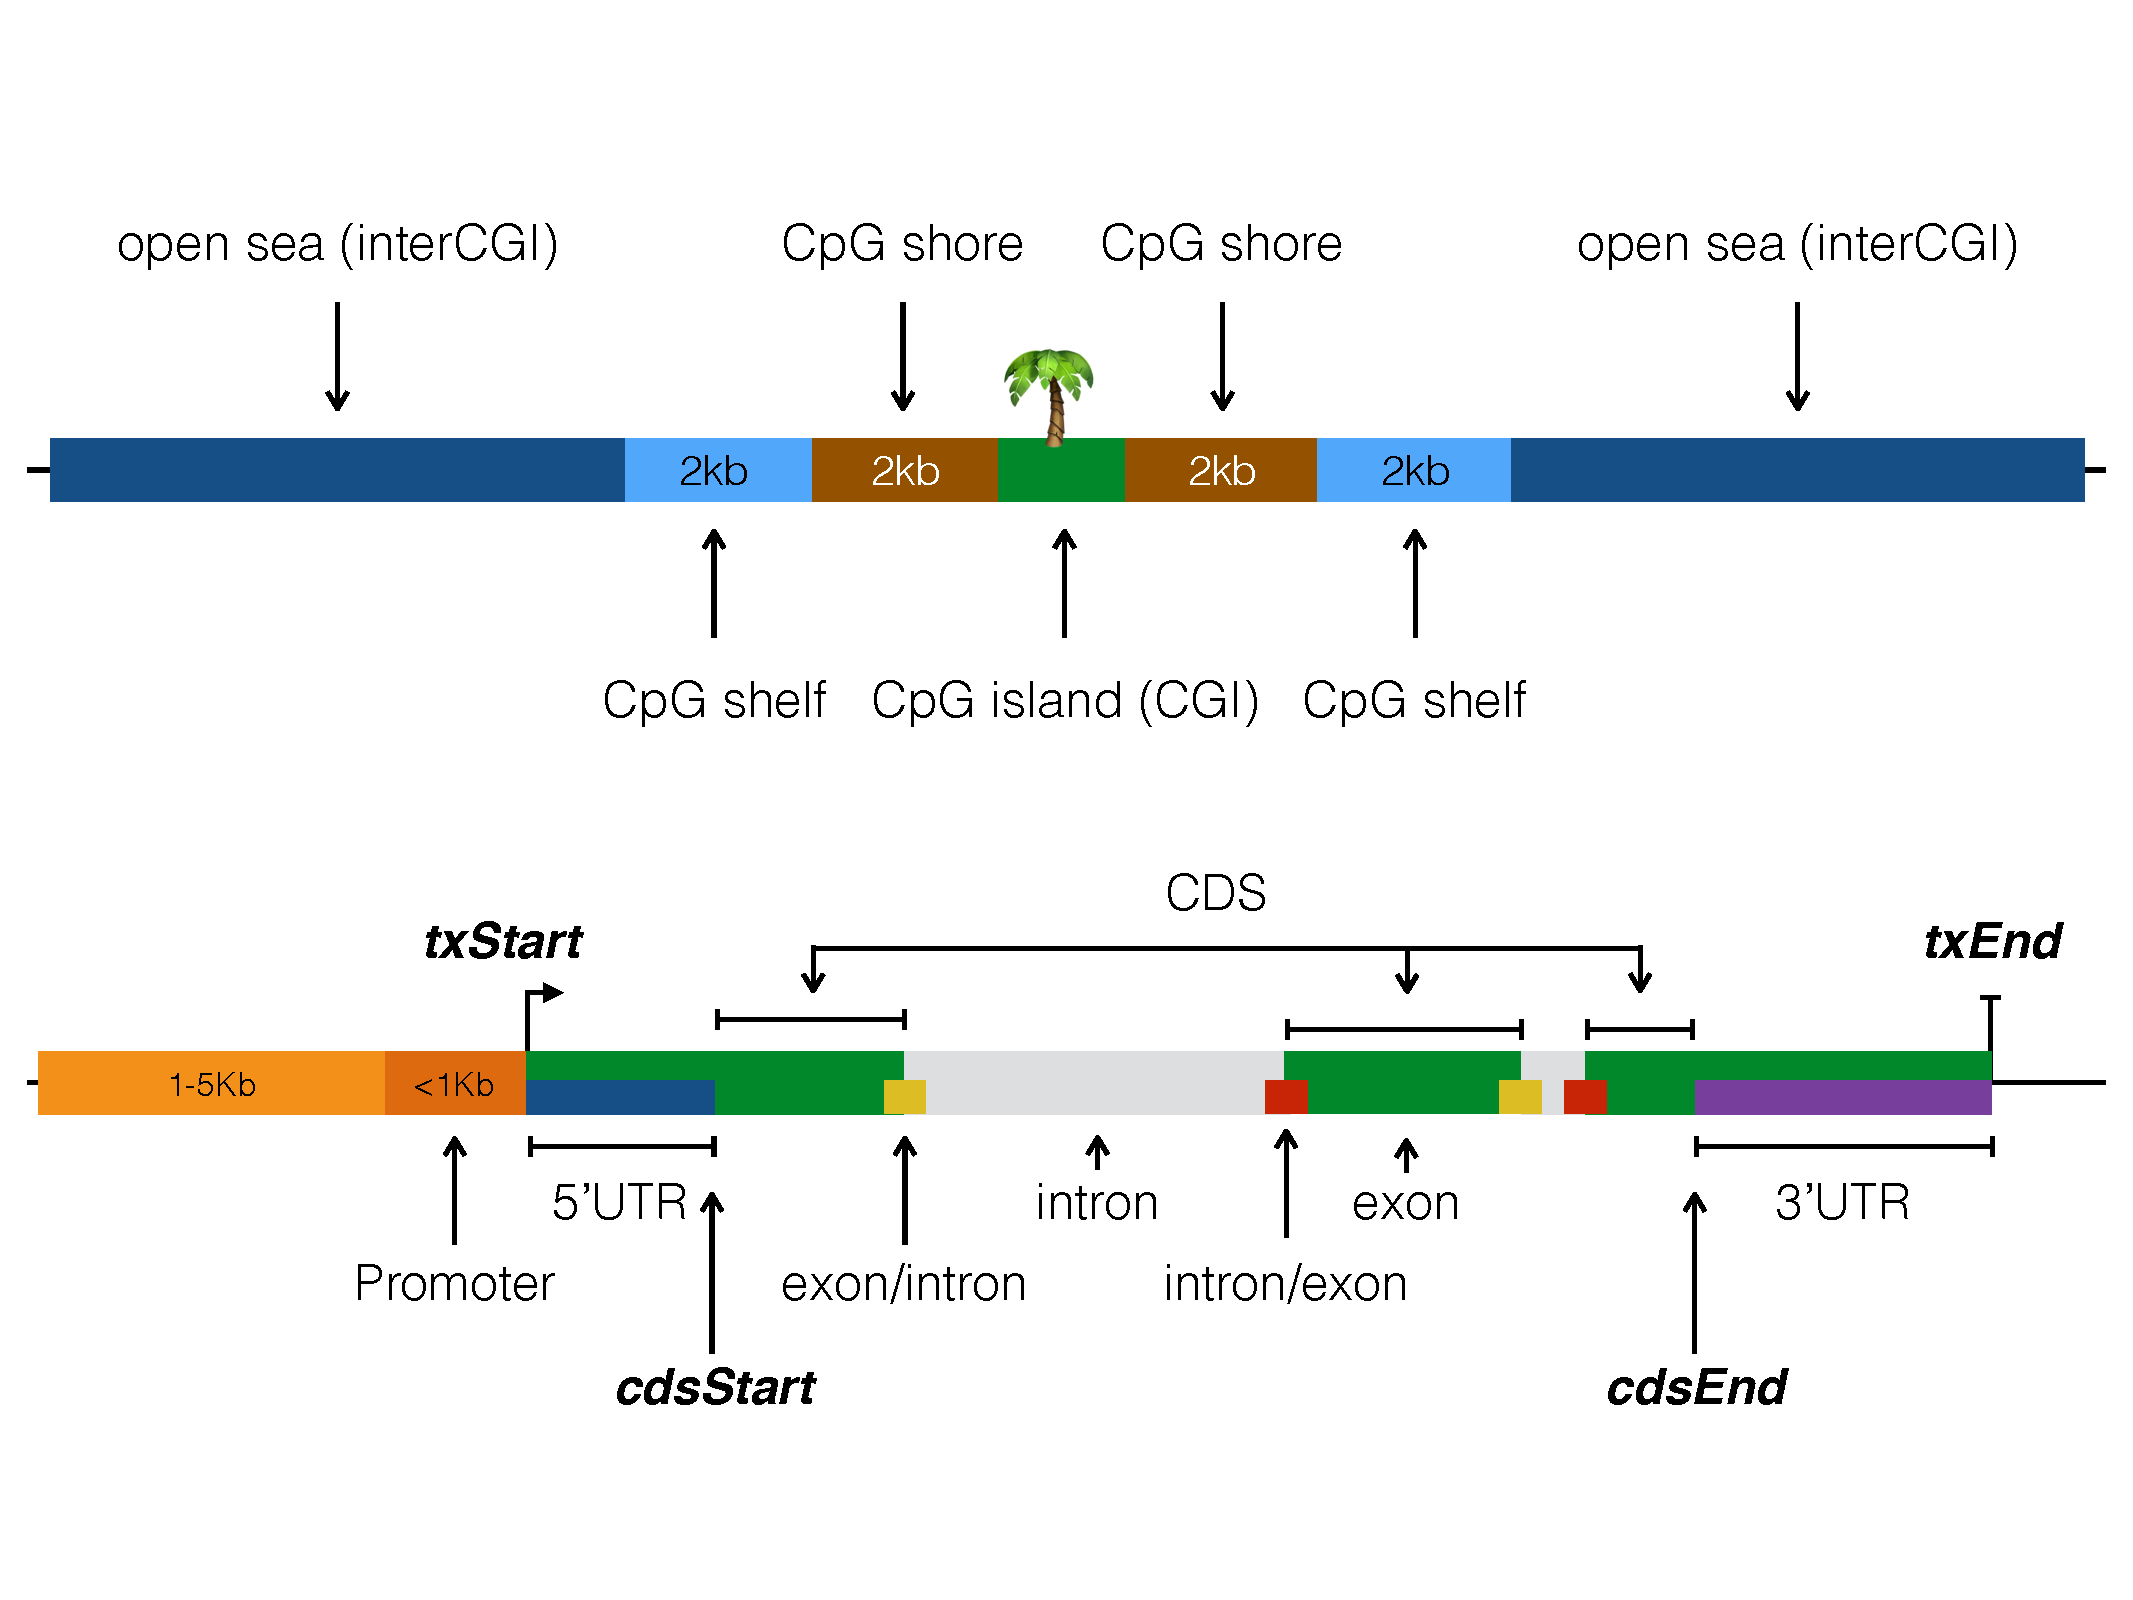
\includegraphics[width=1\textwidth]{chap4figs/figure4_1.pdf}
\caption[Schematics of the CpG and genic annotation types used.]
{
% Rackham requires the figure list title matches the first sentence, so repeat that sentence here
\textbf{Schematics of the CpG and genic annotation types used.} (Top) Schematic of the UCSC CpG annotations used in annotatr. The CpG islands are retrieved from either the AnnotationHub R package or the UCSC Golden Path, depending on availability for the genome build. CpG shores are defined as the 2kb extension upstream and downstream of the CpG island boundaries, less any CpG islands. The CpG shelves are a further 2kb extension upstream and downstream of the furthest upstream and downstream boundaries of the CpG shores, less any CpG island and shore annotations. The complement of the CpG islands, shores, and shelves make up the "open sea" or interCGI annotation. (Bottom) A schematic of the genic annotations available in annotatr. Functions from the GenomicFeatures R package in conjunction with custom functions are used to extract regions 1-5Kb upstream of a TSS, promoters, 5'UTRs, exons, introns, and 3'UTRs. Additionally, exon/intron and intron/exon boundaries are determined by 200bp regions around such boundaries. Annotations may overlap one another from the same or from different transcripts. Genic annotations always have UCSC Transcript IDs and Entrez Gene IDs and gene symbols when applicable.
}
\label{chap4:fig:1}
\end{figure}

\newpage

\begin{figure}[!ht]

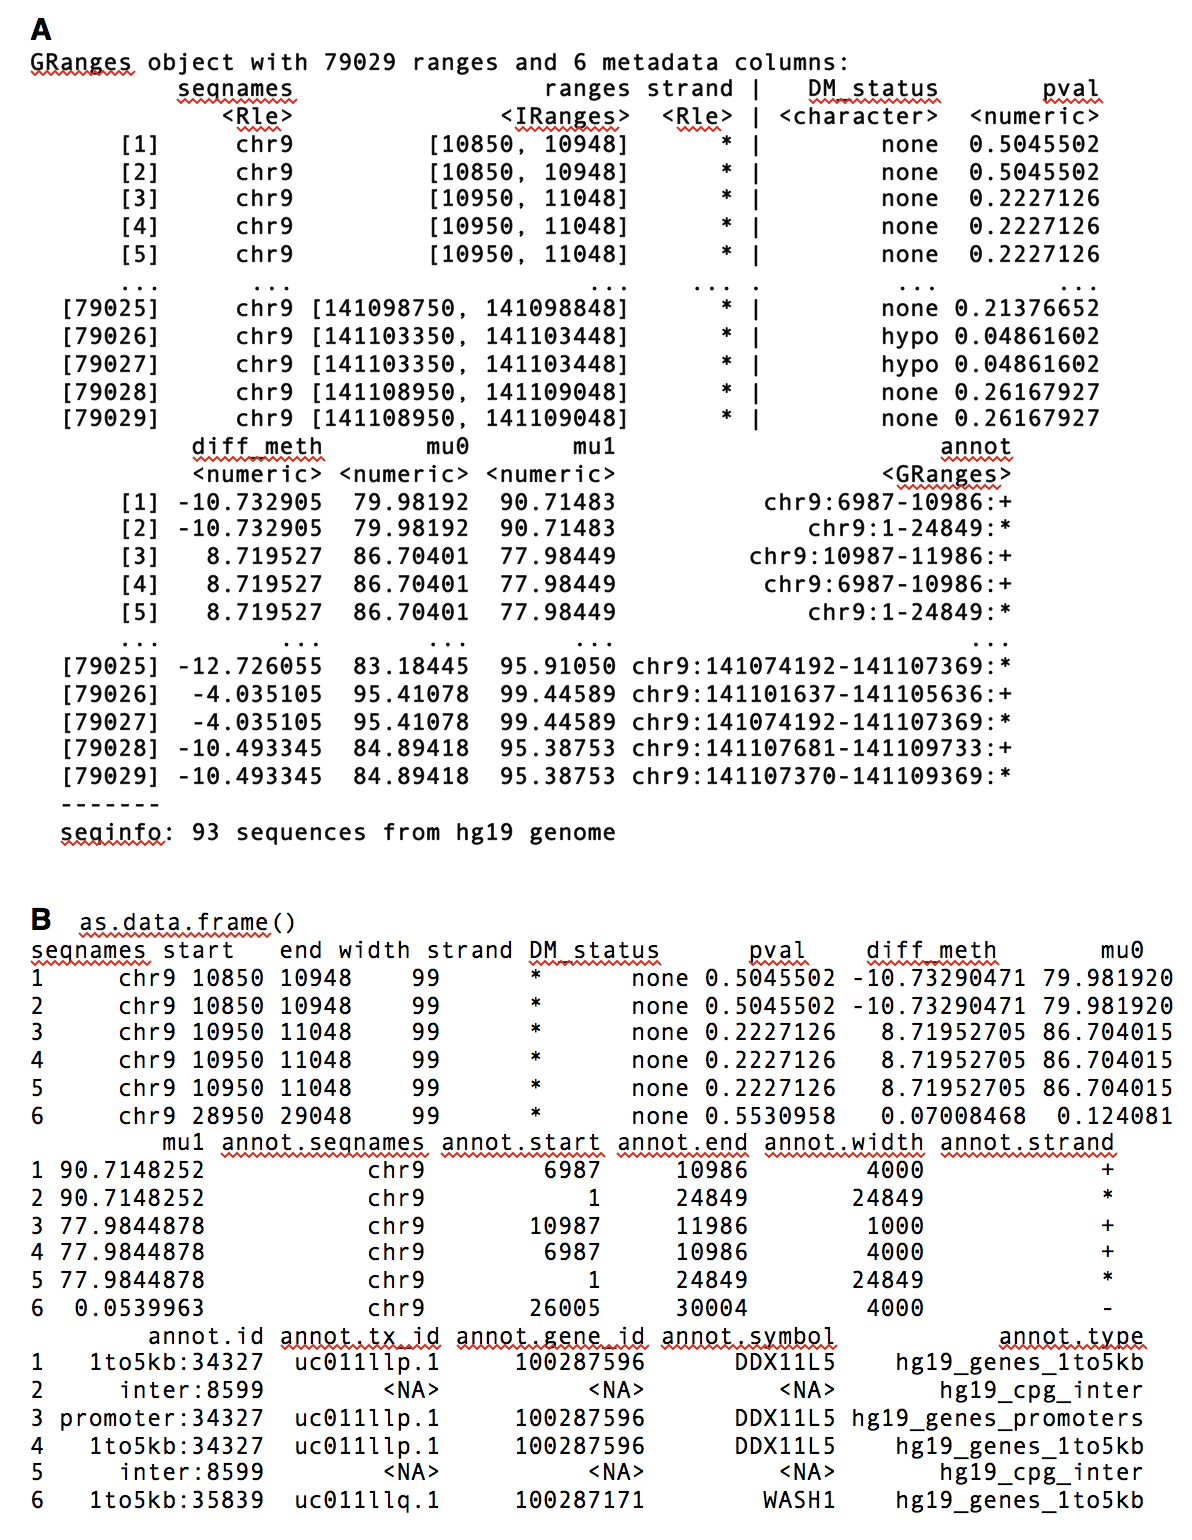
\includegraphics[width=0.8\textwidth]{chap4tables/table4_3.png}
\caption[Example output of the annotate\_regions() function as a GRanges object (A) and data.frame (B).]
{
% Rackham requires the figure list title matches the first sentence, so repeat that sentence here
\textbf{Example output of the annotate\_regions() function as a GRanges object (A) and data.frame (B).}
(A) Output of GRanges object with extra columns containing extra data from the input regions (DM\_status, pval, diff\_meth, mu0, and mu1). In addition, a column giving complete details about the annotations is in the annot column, however the gene information is hidden in this output. Of note is that regions with multiple annotations are repeated (see rows 1-2 and 3-5). (B) Using data.frame() allows users to coerce this GRanges object into a flat table and expose the gene information (last five columns).
}
\label{chap4:table:3}

\end{figure}

\newpage

\begin{figure}[ht!]
\centering
% manually adjust the width of the figure
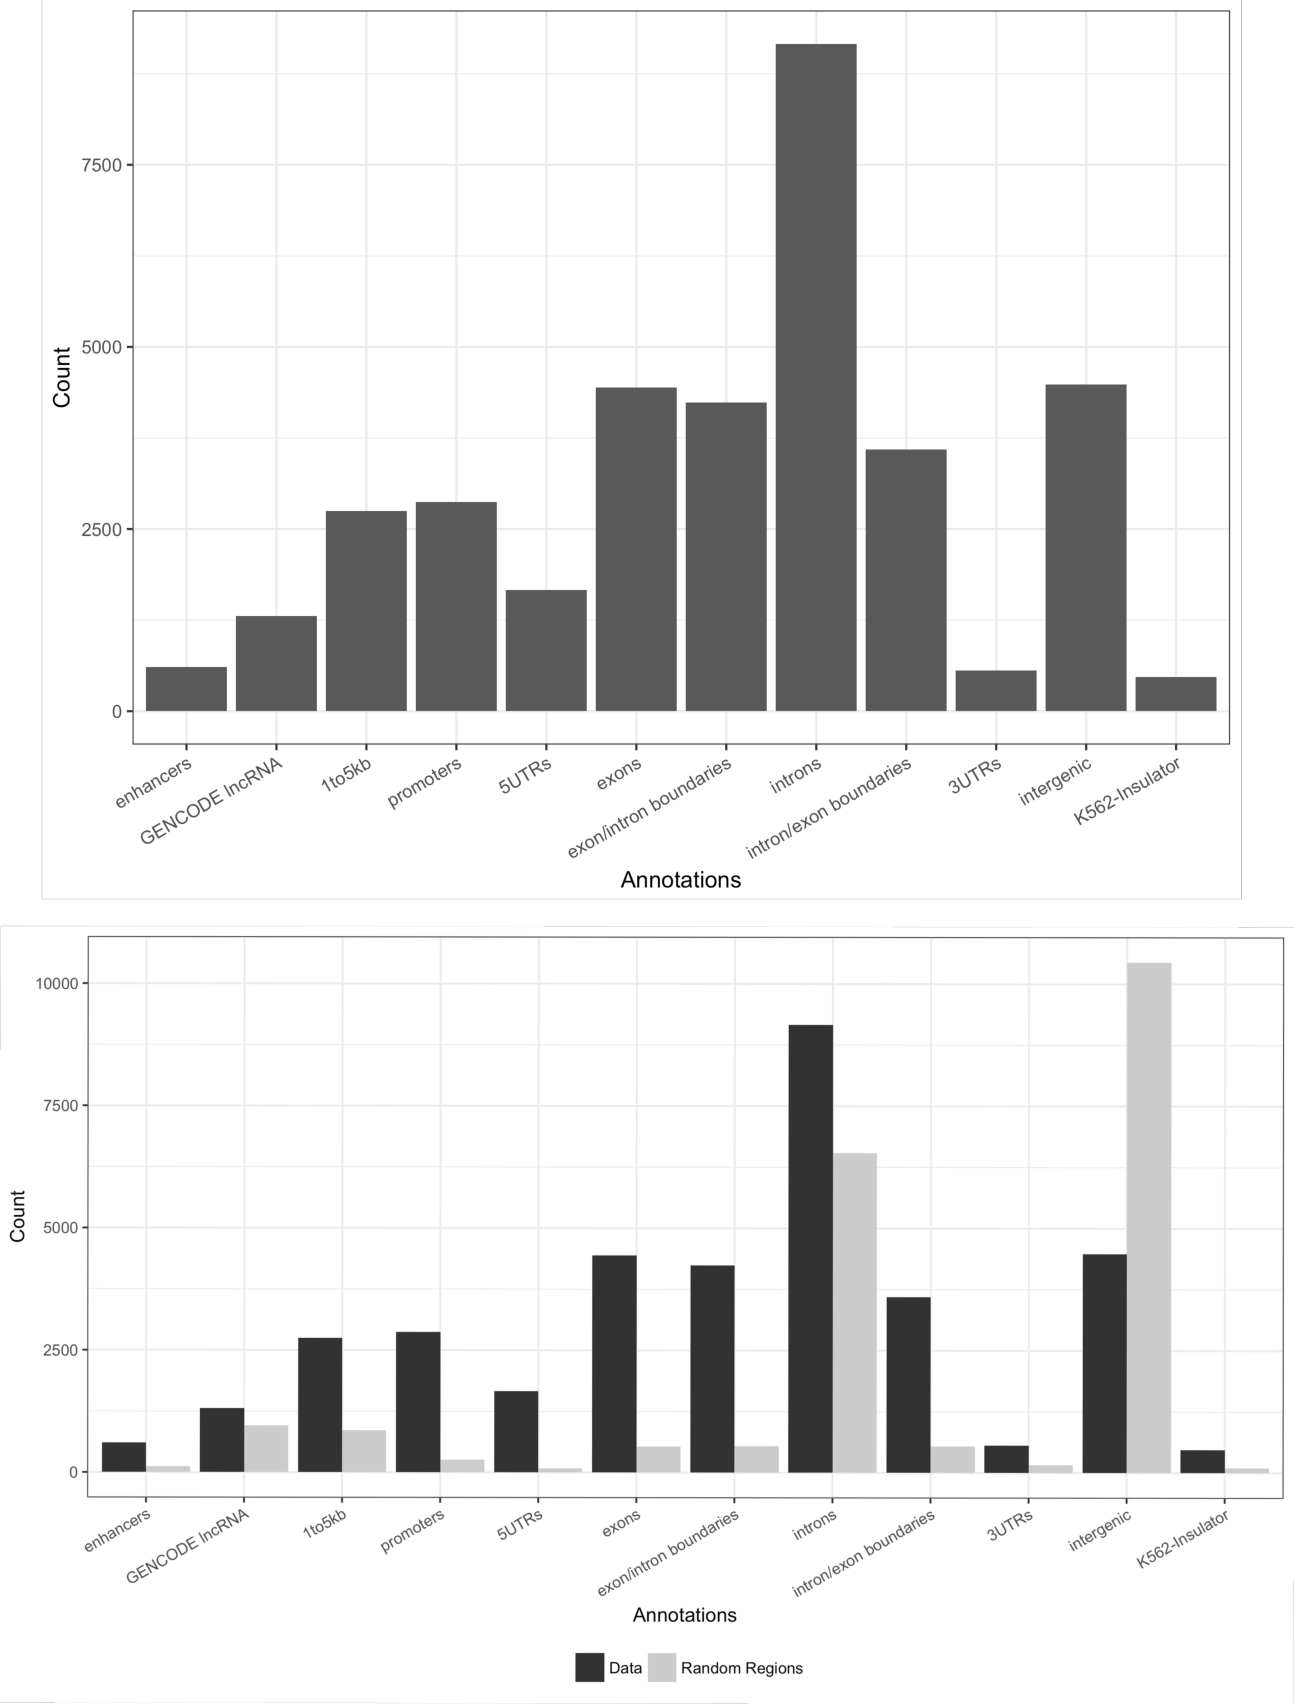
\includegraphics[width=1\textwidth]{chap4figs/figure4_2.pdf}
\caption[Examples of annotatr barplots.]
{
% Rackham requires the figure list title matches the first sentence, so repeat that sentence here
\textbf{Examples of barplots.} The counts of regions per annotation type (top), and with annotations of random regions for comparison (bottom). In (bottom) we note that many annotations appear to be enriched (enhancers, promoters, exon/intron boundaries, and K562-insulators, and only intergenic regions are depleted. All plots are based on the ggplot2 package (Wickham, 2009).
}
\label{chap4:fig:2}
\end{figure}

\newpage

\begin{figure}[ht!]
\centering
% manually adjust the width of the figure
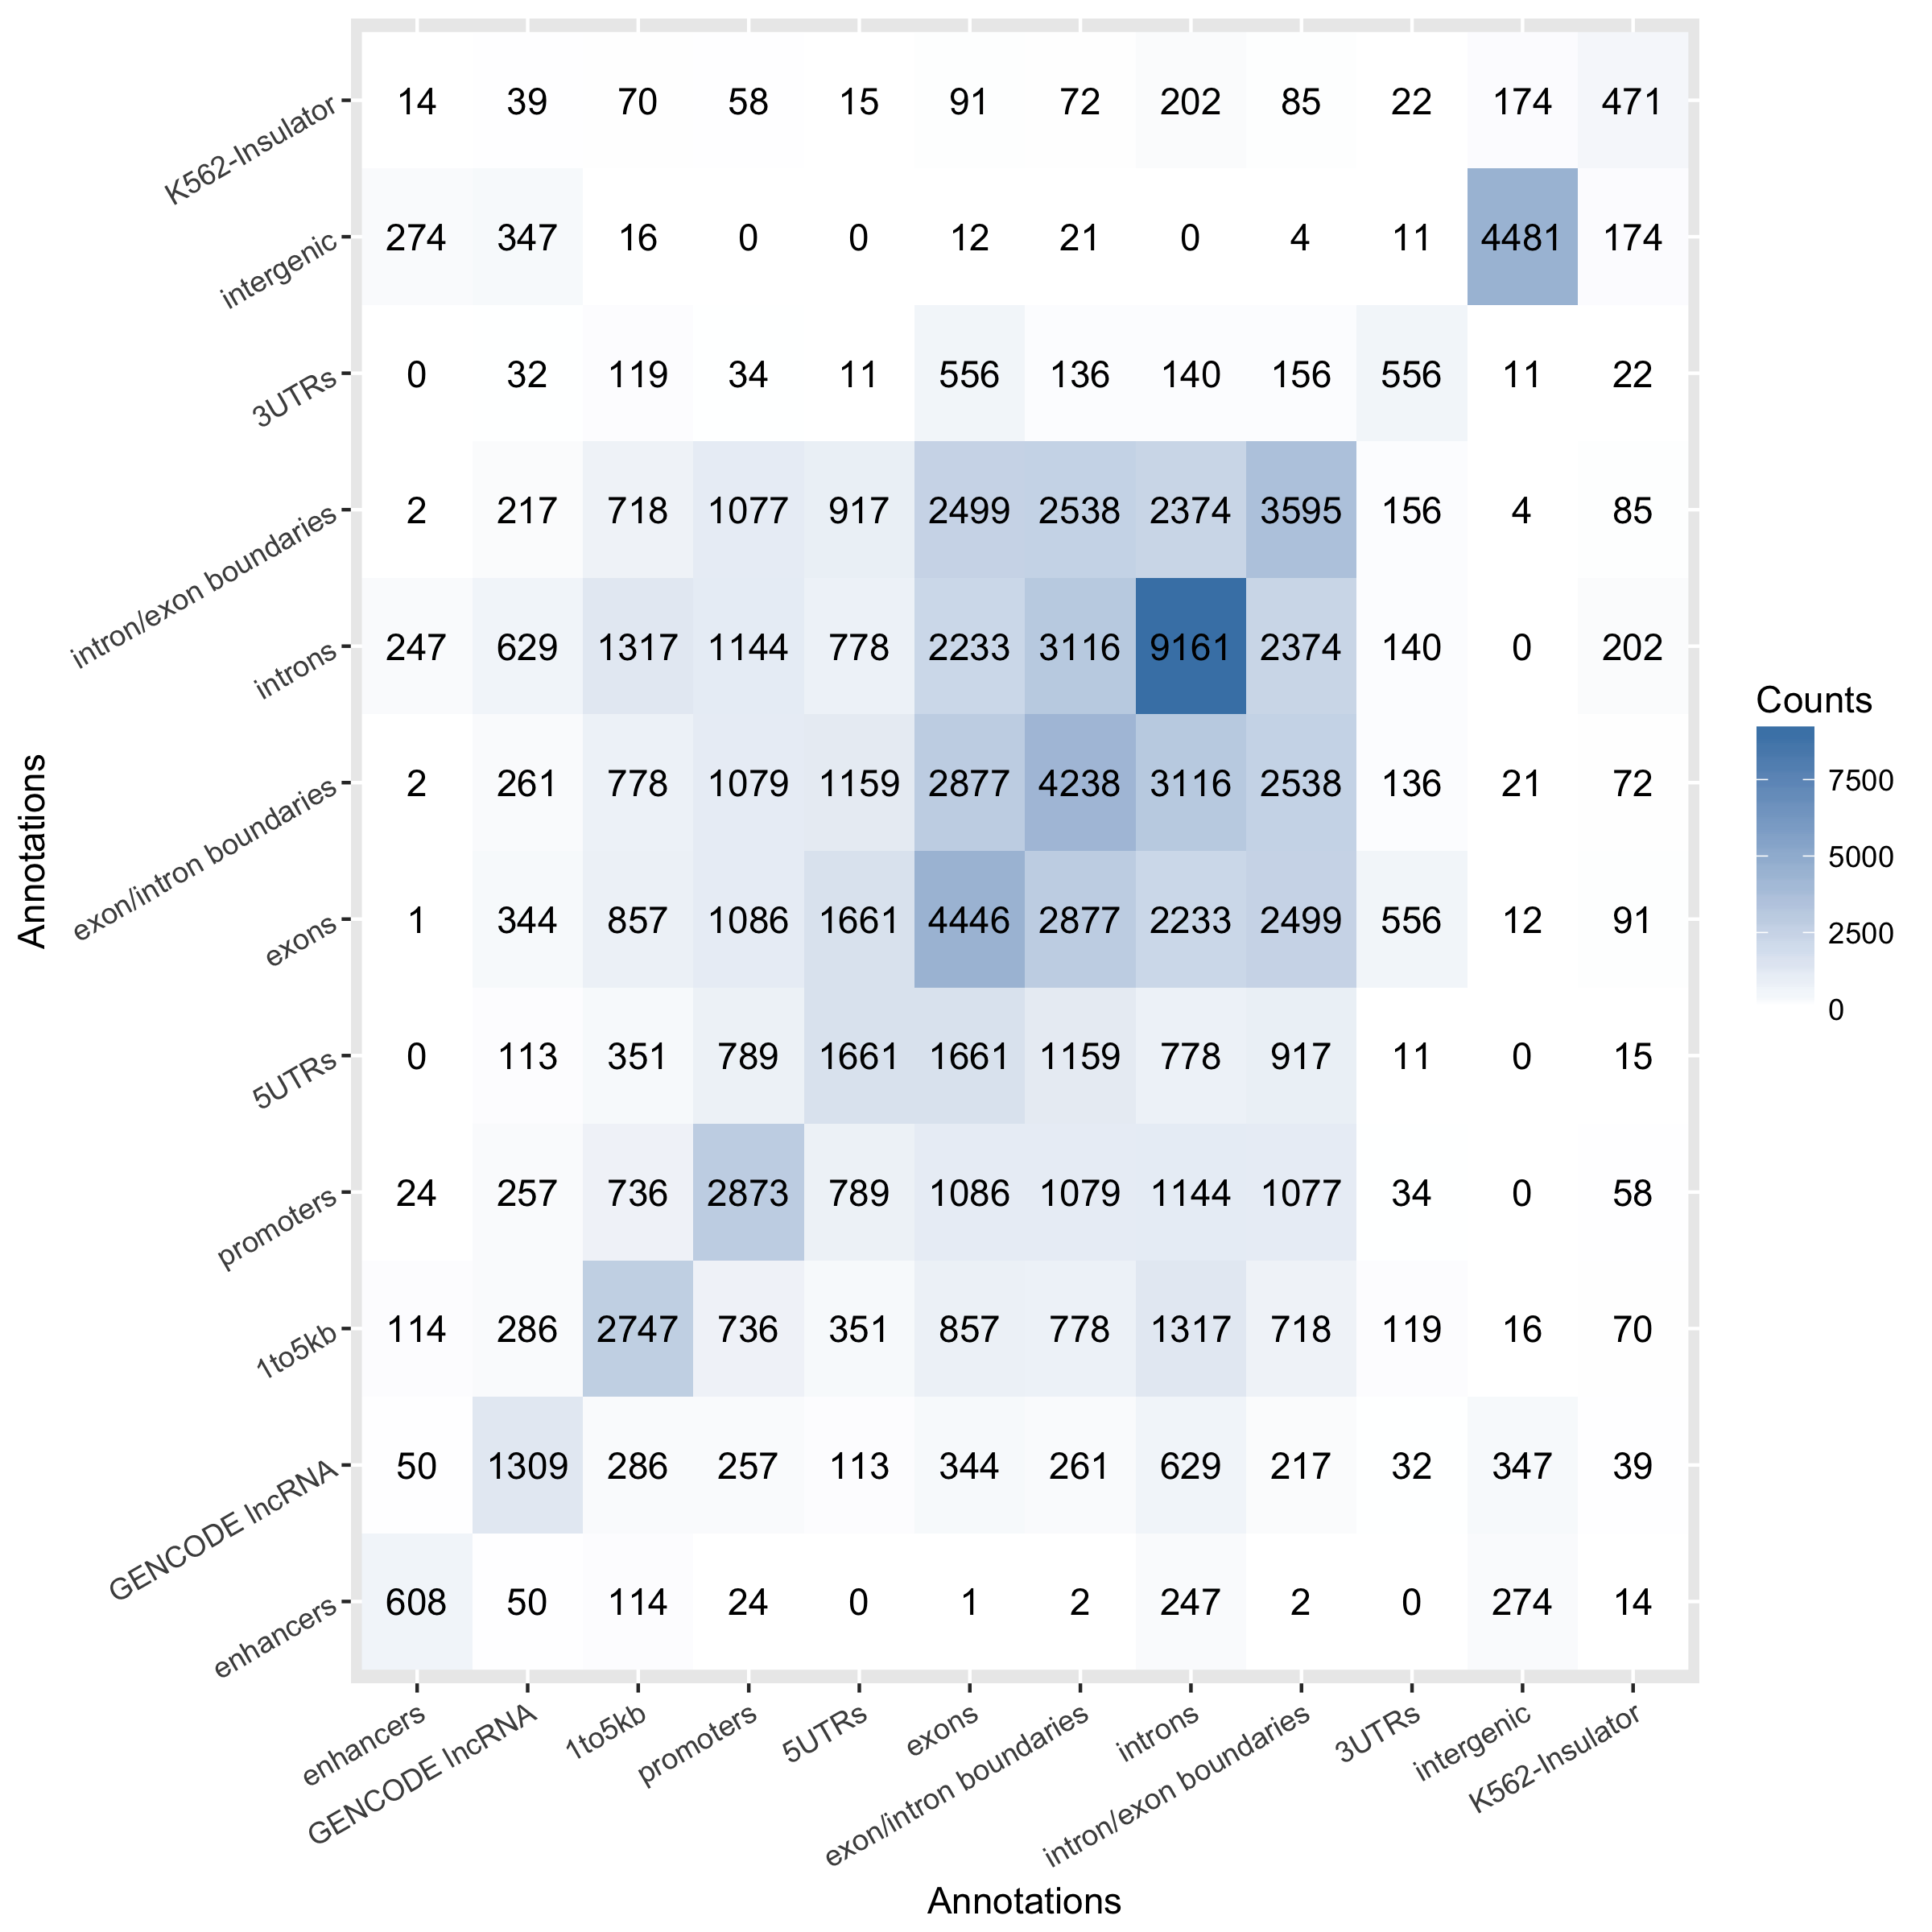
\includegraphics[width=1\textwidth]{chap4figs/figure4_3.png}
\caption[Example of annotatr coannotation heatmap.]
{
% Rackham requires the figure list title matches the first sentence, so repeat that sentence here
\textbf{Example of coannotation heatmap.} The number of input genomic regions occurring in intersections of annotation pairs. This visualization is helpful for prioritizing types of regions to examine in more detail. For example, there are 247 regions that are in an enhancer and reside in an intron.
}
\label{chap4:fig:3}
\end{figure}

\newpage

\begin{figure}[ht!]
\centering
% manually adjust the width of the figure
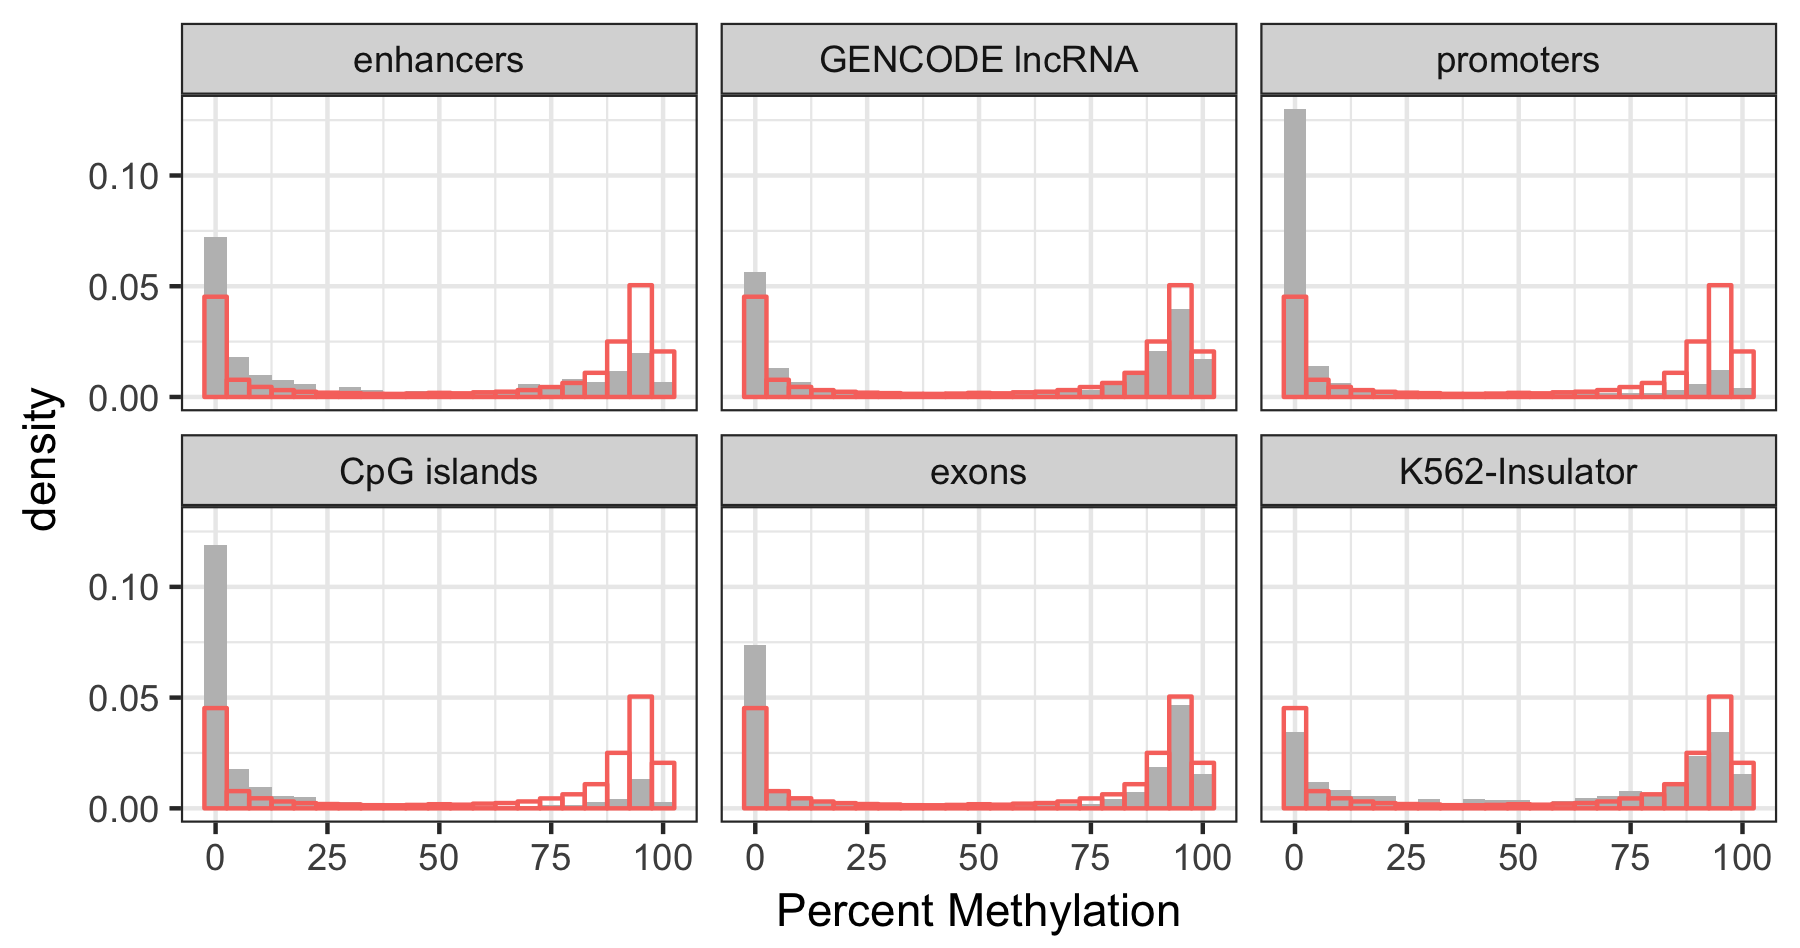
\includegraphics[width=1\textwidth]{chap4figs/figure4_4.png}
\caption[Example of numerical distributions.]
{
% Rackham requires the figure list title matches the first sentence, so repeat that sentence here
\textbf{Example of numerical distributions.} The distribution of the methylation rate across annotations (solid) with the background distribution (outline). Note the clearly visible hyper- and hypo-methylation trends in the different annotation types.
}
\label{chap4:fig:4}
\end{figure}

\newpage

\begin{figure}[ht!]
\centering
% manually adjust the width of the figure
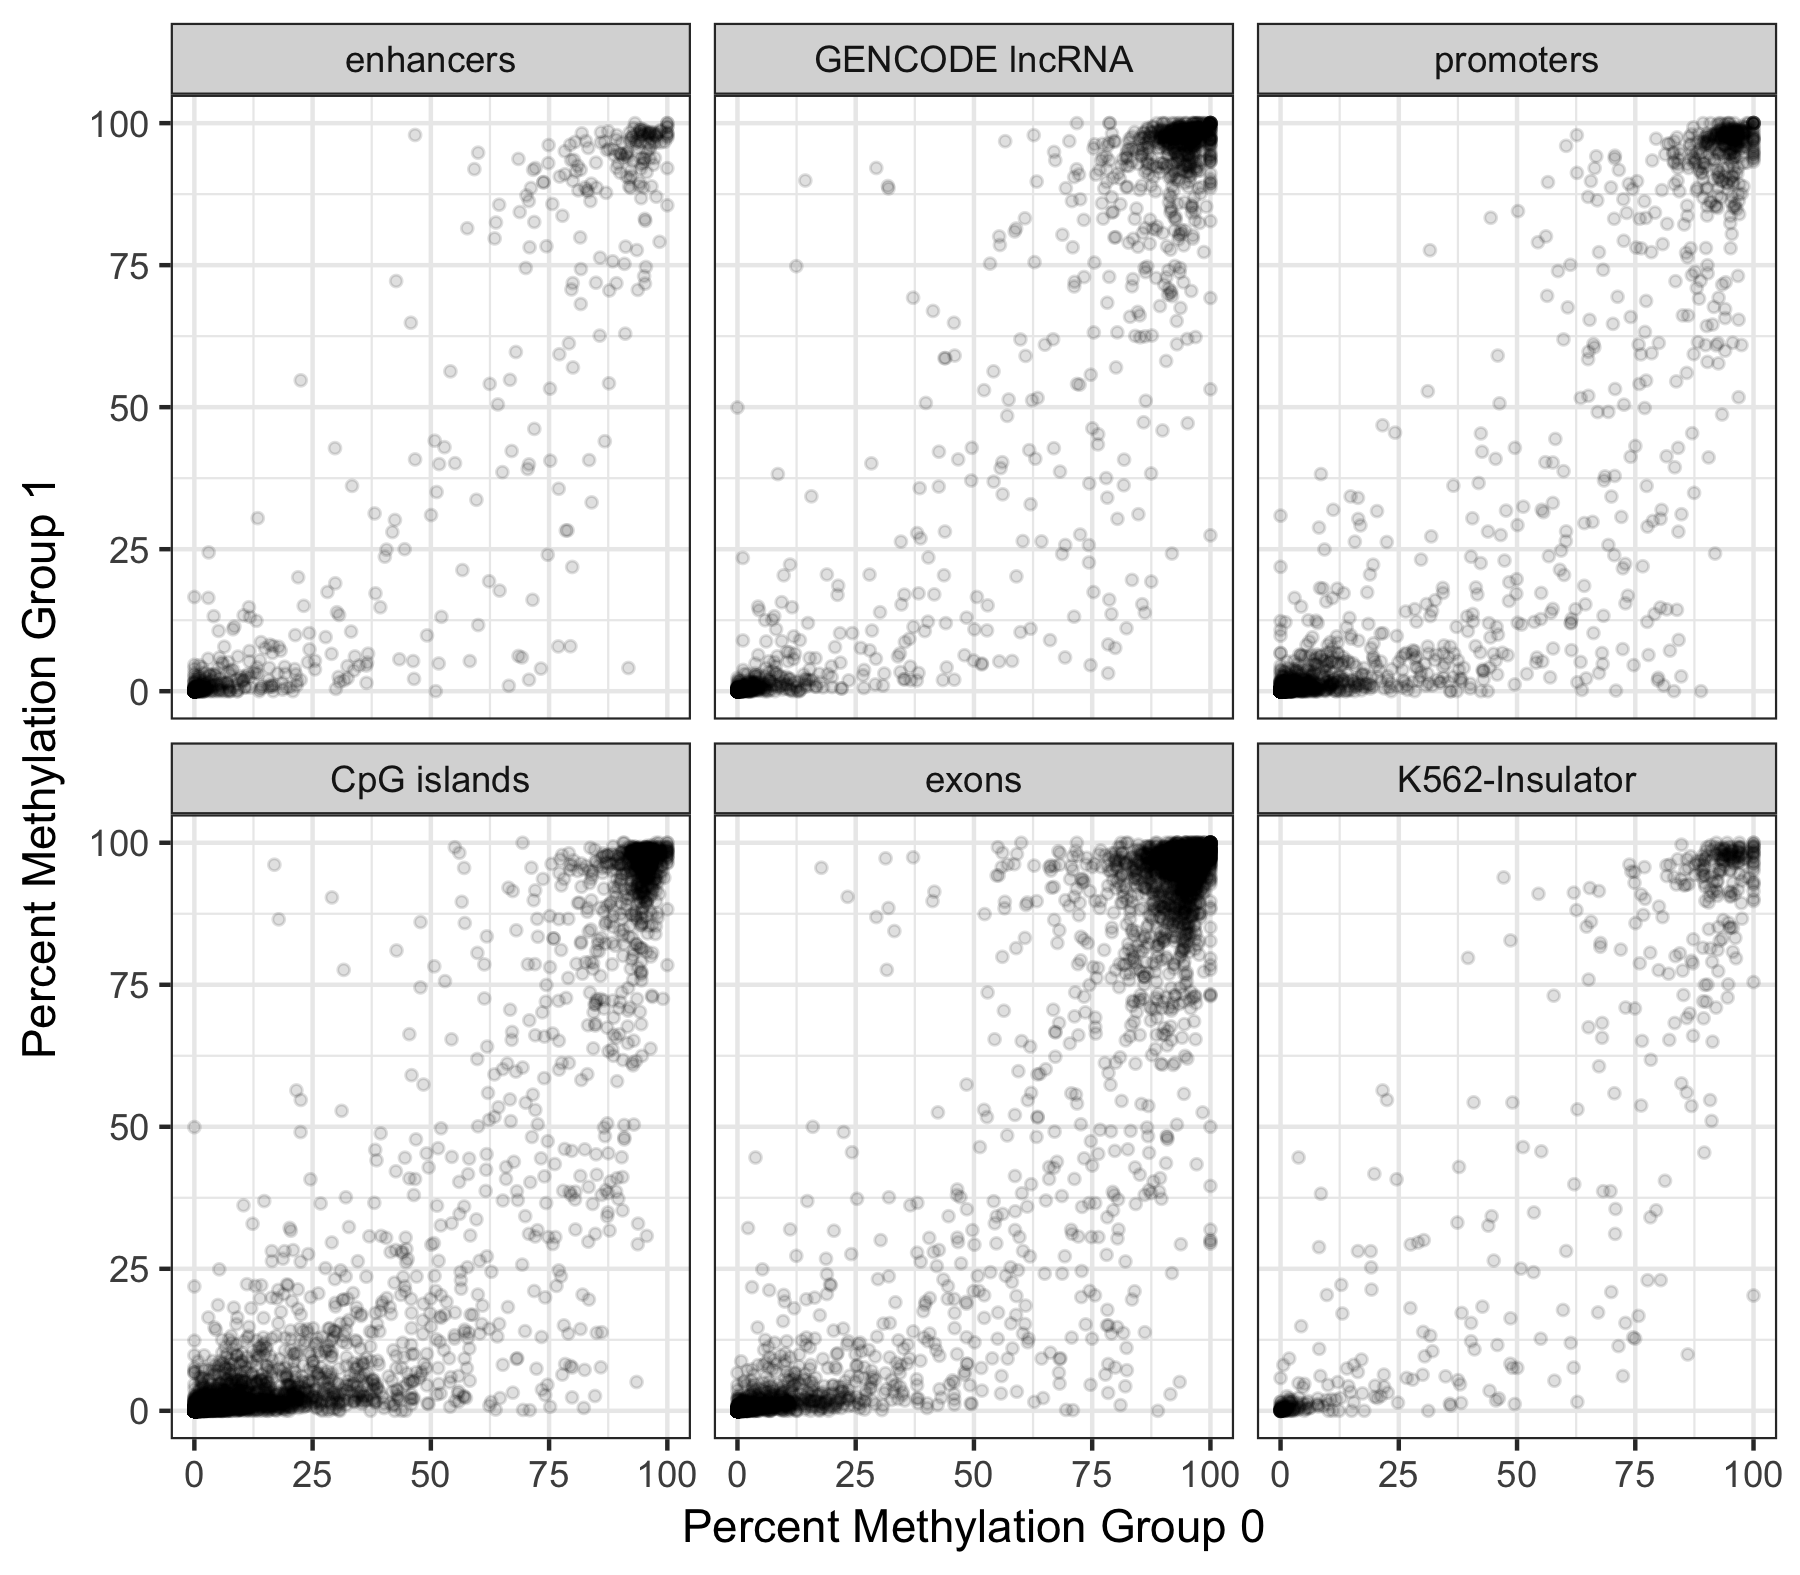
\includegraphics[width=1\textwidth]{chap4figs/figure4_5.png}
\caption[Example of scatterplots.]
{
% Rackham requires the figure list title matches the first sentence, so repeat that sentence here
\textbf{Example of scatterplots.} Scatter plots of methylation rates comparing two sample groups across a subset of the annotation types. This visualization enables quick assessment of correlations in numerical data across different annotations types (or categorical variables).
}
\label{chap4:fig:5}
\end{figure}

\newpage

\begin{figure}[ht!]
\centering
% manually adjust the width of the figure
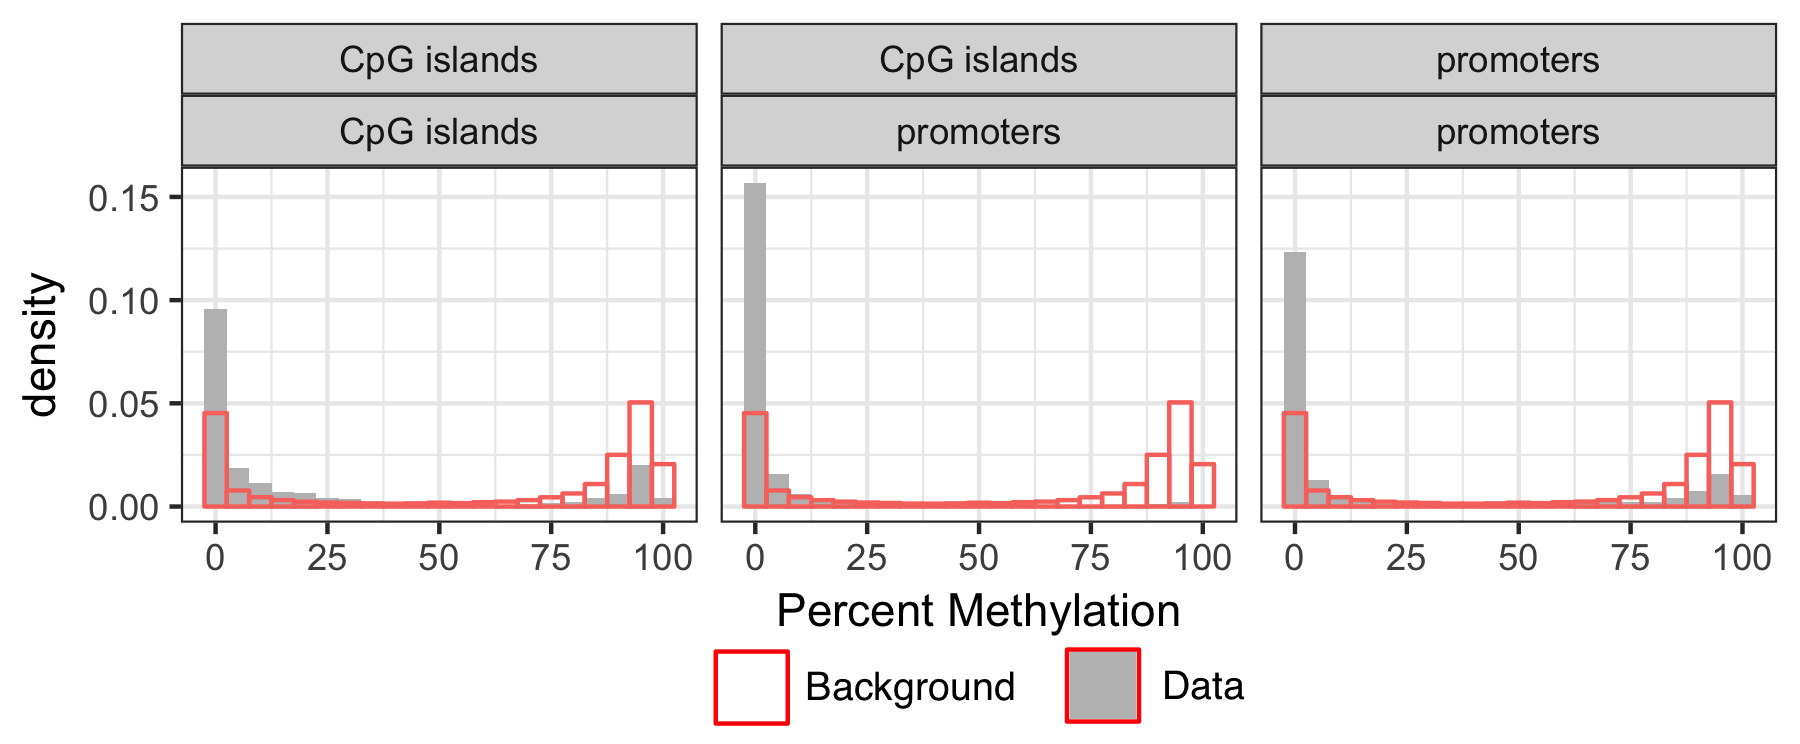
\includegraphics[width=1\textwidth]{chap4figs/figure4_6.png}
\caption[Example of numerical coannotations.]
{
% Rackham requires the figure list title matches the first sentence, so repeat that sentence here
\textbf{Example of numerical coannotations.} The distribution of the methylation rate of regions in just CpG islands (left), promoters and CpG islands (middle), and just promoters (right). Note the relative hypermethylation trend in the co-annotated regions compared to the singly annotated regions.
}
\label{chap4:fig:6}
\end{figure}

\newpage

\begin{figure}[ht!]
\centering
% manually adjust the width of the figure
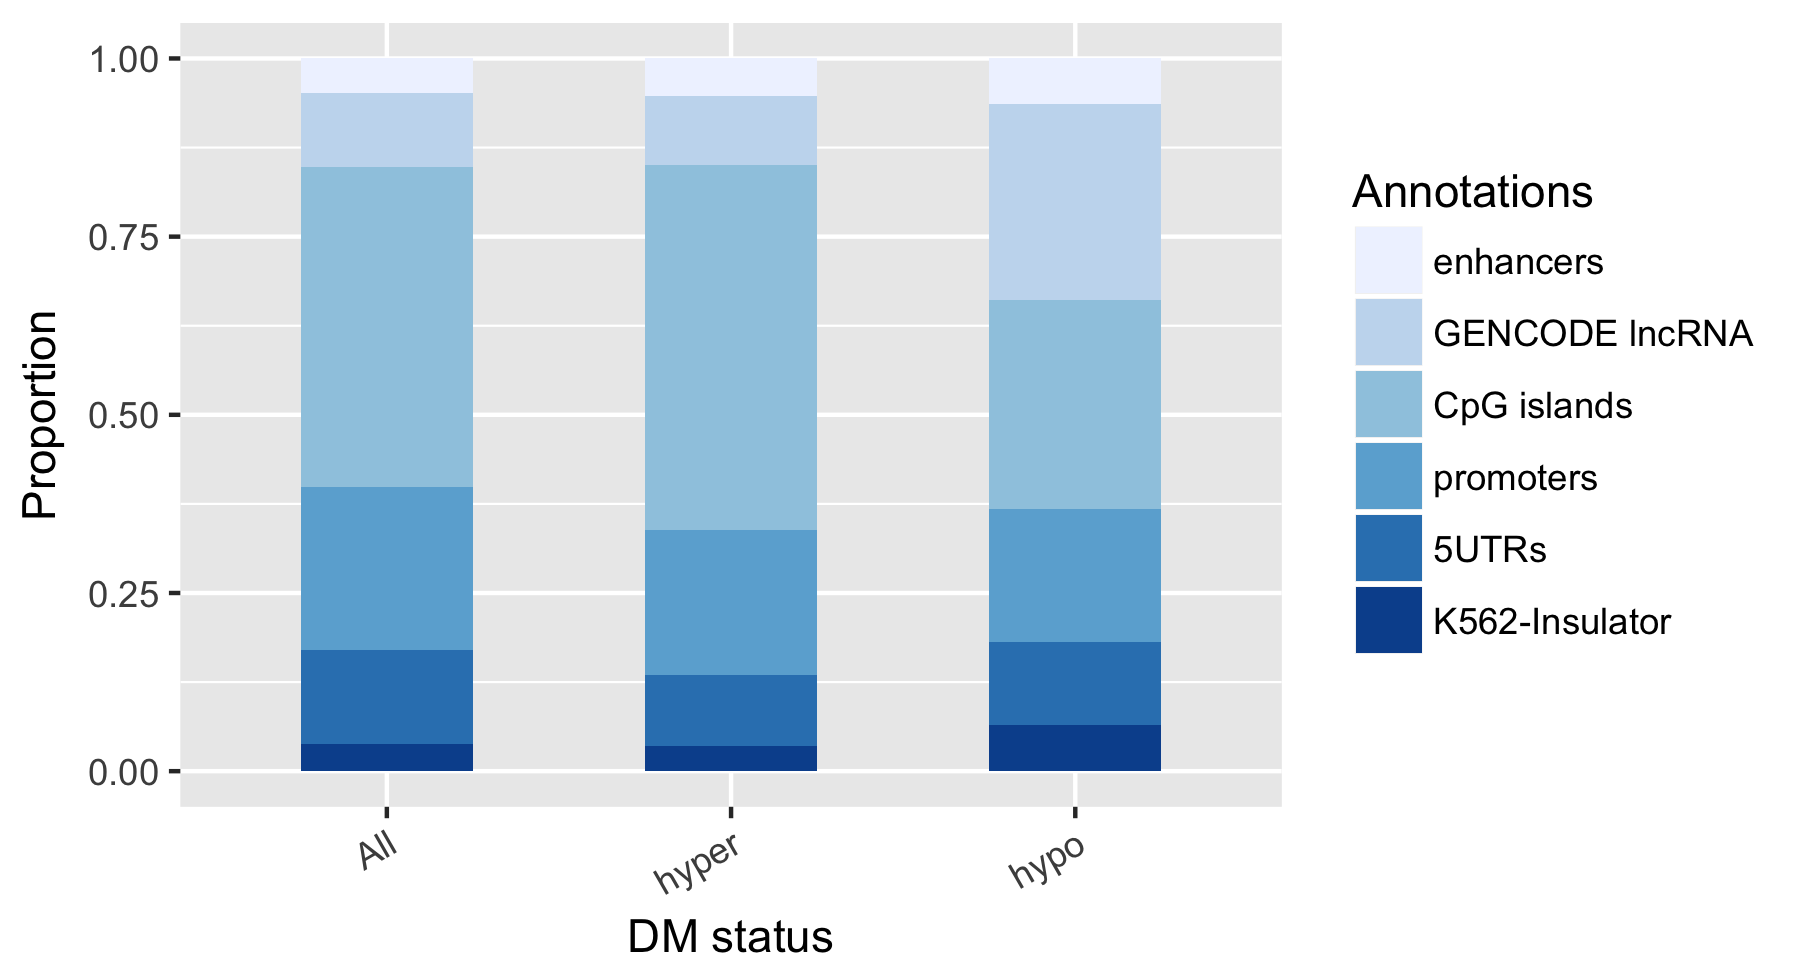
\includegraphics[width=1\textwidth]{chap4figs/figure4_7.png}
\caption[Example of categorical annotations.]
{
% Rackham requires the figure list title matches the first sentence, so repeat that sentence here
\textbf{Example of categorical annotations.} The proportion of annotations of hyper- and hypo-methylated regions, with the background distribution (All) for comparison. Note the differences in enhancers, CpG islands, lncRNAs, and K562-insulators between hyper- and hypo-methylated regions compared to each other and all tested regions.
}
\label{chap4:fig:7}
\end{figure}

\newpage

\begin{figure}[ht!]
\centering
% manually adjust the width of the figure
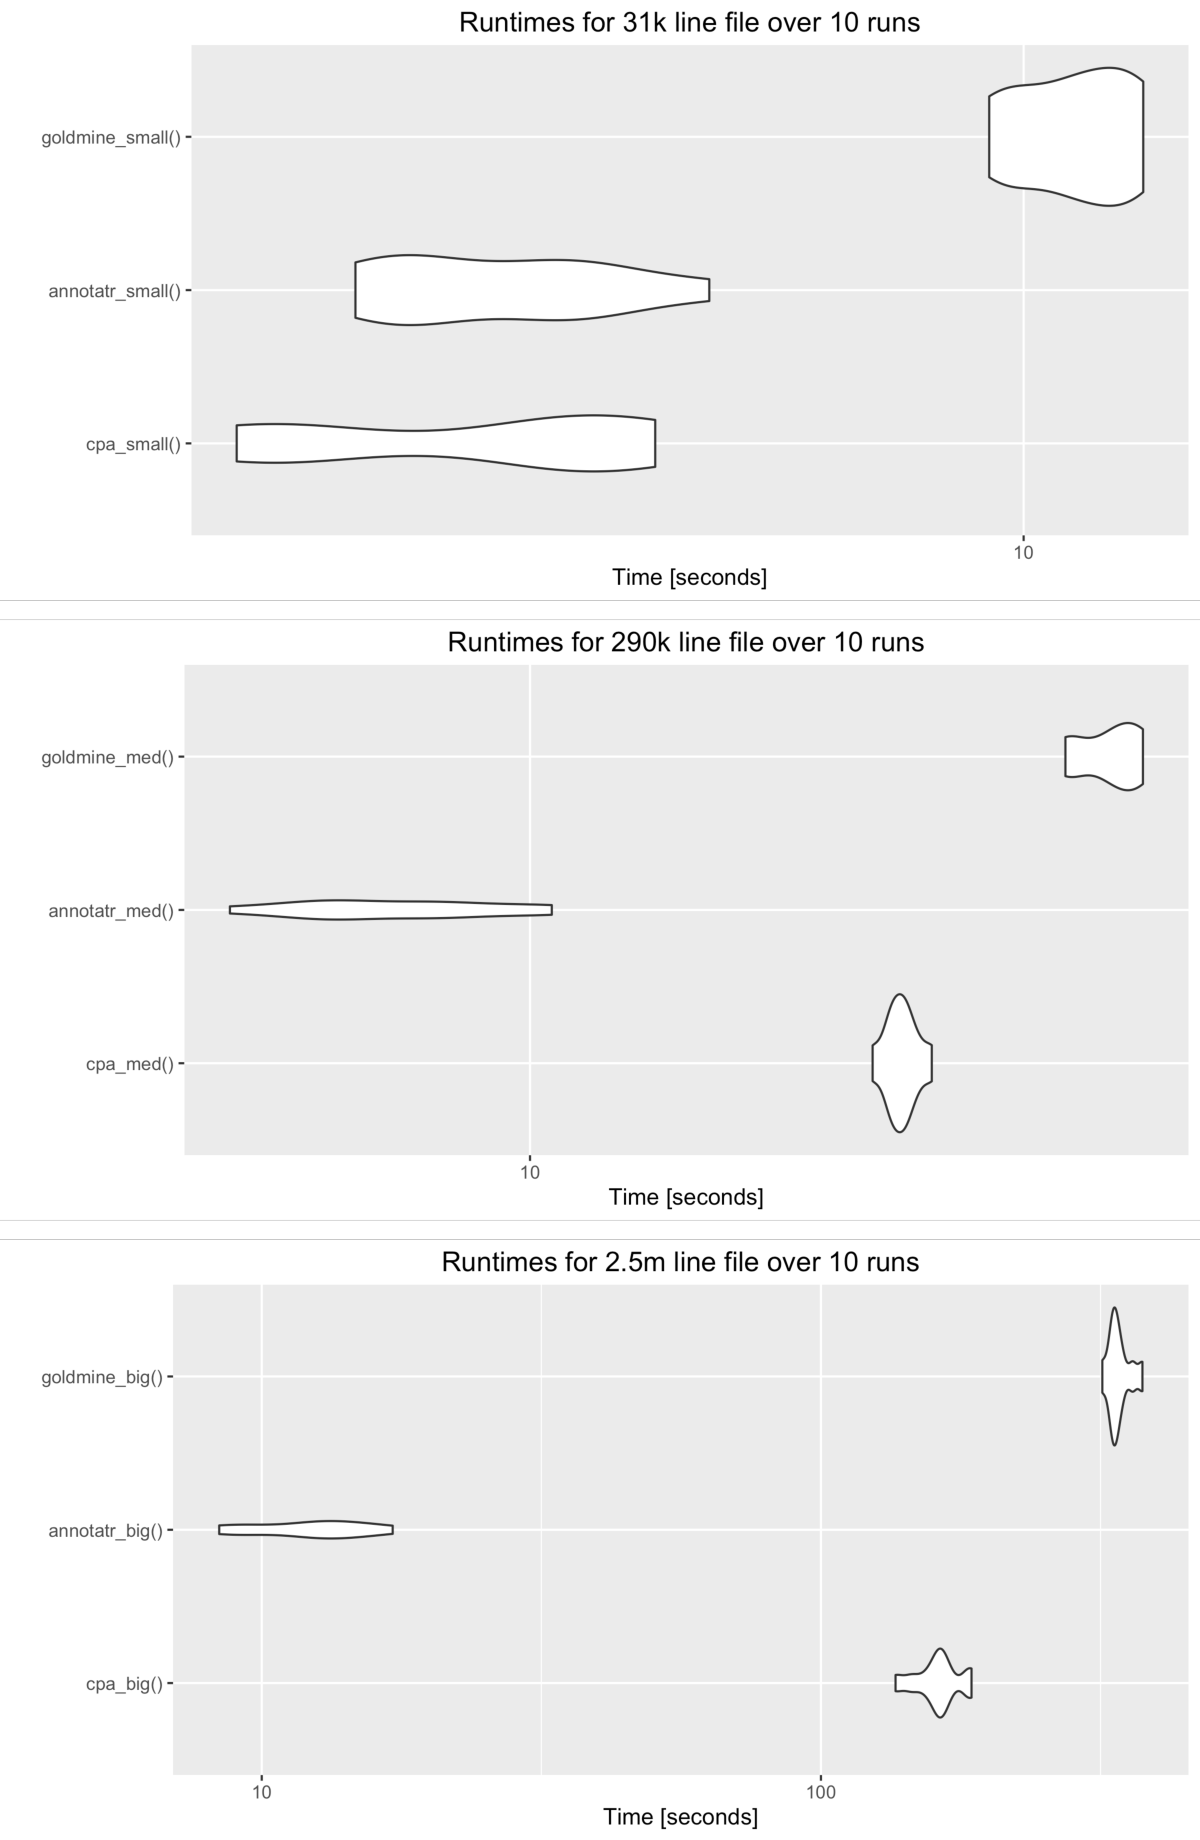
\includegraphics[width=0.8\textwidth]{chap4figs/figure4_8.pdf}
\caption[Benchmarking results for annotatr.]
{
% Rackham requires the figure list title matches the first sentence, so repeat that sentence here
\textbf{Benchmarking results for annotatr.} Violin plots of benchmarking results comparing annotatr to ChIPpeakAnno and goldmine from file read to annotation for small (31k, Top), medium (265k, Middle), and large (2.5m, Bottom) files over 10 runs. Both annotatr and ChIPpeakAnno perform about the same for small files (Top), but for larger files annotatr is clearly faster (Middle) and (Bottom).
}
\label{chap4:fig:8}
\end{figure}

\clearpage
\section*{Tables}
\begin{table}[!ht]
\centering
\small
\begin{tabular}{l|ll}
\textbf{Annotation Type} & \textbf{Organism}      & \textbf{Genome Builds}                         \\\hline
\textbf{Genic}           & Fly, Human, Mouse, Rat & dm3, dm6, hg19, hg38, mm9, mm10, rn4, rn5, rn6 \\
\textbf{CpG}             & Human, Mouse, Rat      & hg19, hg38, mm9, mm10, rn4, rn5, rn6           \\
\textbf{lncRNA}          & Human, Mouse           & hg19, hg38, mm10                               \\
\textbf{Enhancers}       & Human, Mouse           & hg19, hg38, mm9, mm10                          \\
\textbf{Chromatin State} & Human                  & hg19
\end{tabular}
\normalsize
\caption[A summary of annotations available for organisms and genome builds.]
{
% Rackham requires the figure list title matches the first sentence, so repeat that sentence here
\textbf{A summary of annotations available for organisms and genome builds.}
Custom annotations may be used in conjunction with built-in annotations, or for organisms with no built-in annotations. Note, enhancers for hg38 and mm10 use the rtracklayer::liftOver() function on enhancers from hg19 and mm9, respectively.
}
\label{chap4:table:1}

\end{table}

\newpage

\begin{table}[!ht]
\small
\centering
\begin{tabular}{lllllllll}
\textbf{chr} & \textbf{start} & \textbf{end} & \textbf{DM\_status} & \textbf{pval} & \textbf{strand} & \textbf{mu0} & \textbf{mu1} & \textbf{diff\_meth} \\
chr9         & 10849          & 10948        & none                & 0.505         & *               & -10.73       & 79.98        & 90.71               \\
chr9         & 10949          & 11048        & none                & 0.223         & *               & 8.72         & 86.7         & 77.98               \\
chr9         & 28949          & 29048        & none                & 0.553         & *               & 0.07         & 0.12         & 0.05                \\
chr9         & 72849          & 72948        & hyper               & 0.012         & *               & 44.88        & 72.46        & 27.58               \\
chr9         & 72949          & 73048        & none                & 0.175         & *               & 17.76        & 28.44        & 10.68               \\
chr9         & 73049          & 73148        & hyper               & 0.029         & *               & 3.8          & 4.14         & 0.34                \\
chr9         & 73149          & 73248        & none                & 0.28          & *               & 1.62         & 2.21         & 0.59                \\
chr9         & 73349          & 73448        & none                & 0.19          & *               & -1.05        & 0            & 1.05
\end{tabular}
\normalsize
\caption[Example of a BED6$+$ file used for input into annotatr.]
{
% Rackham requires the figure list title matches the first sentence, so repeat that sentence here
\textbf{Example of a BED6$+$ file used for input into annotatr.}
The BED6 format has 6 required columns in the following order: chr, start, end, name, score, and strand. Annotatr can interpret BED files with any number of columns after these 6 (the $+$), so long as they are named and their type is explicitly given (see ?annotatr::read\_regions for details). The underlying rtracklayer::import() function can also read files that have the first 3, 4, or 5 columns. Additionally, bedGraph files are supported using the format='bedGraph' parameter. In this example file, the additional columns are used to provide the mean methylation levels of two groups of samples (mu0 and mu1) and the difference in percent methylation between them.
}
\label{chap4:table:2}

\end{table}

\newpage

\begin{table}
\small
\centering
\begin{tabular}{lllll}
\textbf{annot.type}               & \textbf{annot.id}         & \textbf{n} & \textbf{mean} & \textbf{sd} \\
hg19\_genes\_exonintronboundaries & exonintronboundary:301892 & 5          & 3.84          & 4.89        \\
hg19\_genes\_introns              & intron:282469             & 10         & 1.71          & 7.6         \\
hg19\_genes\_introns              & intron:287513             & 3          & -2.55         & 3.07        \\
hg19\_genes\_introns              & intron:289069             & 4          & 0.93          & 7.61        \\
hg19\_genes\_introns              & intron:296414             & 2          & 13.89         & 4.67        \\
hg19\_genes\_introns              & intron:299213             & 3          & -0.13         & 0.41        \\
hg19\_genes\_promoters            & promoter:35271            & 3          & 0.19          & 0.25        \\
hg19\_genes\_promoters            & promoter:37273            & 6          & 10.16         & 15.87
\end{tabular}
\normalsize
\caption[Example of summarized information of a numerical column over the annotations.]
{
% Rackham requires the figure list title matches the first sentence, so repeat that sentence here
\textbf{Example of summarized information of a numerical column over the annotations.}
Shown is a subset of the result of the summarize\_numerical() function by annotation types (annot.type) and the specific annotated regions (annot.id, an internal ID specific to annotatr) over the column containing change in percent methylation (diff\_meth). The input regions are the results of tests for differential methylation as described in the text. Each row is an annotation and contains the average diff\_meth (mean) and standard deviation (sd) over all the input regions intersecting the annotation (the total number of which is n). The annot.id column can be cross referenced with the annotated regions (Table \ref{chap4:table:3}) for information about the specific annot.id (such as Entrez ID or gene symbol) and the n intersecting input regions (such as the exact diff\_meth values for each region).
}
\label{chap4:table:4}

\end{table}

\newpage

\begin{table}[!ht]
\small
\centering
\begin{tabular}{lll}
\textbf{annot.type}             & \textbf{DM\_status} & \textbf{n} \\
hg19\_chromatin\_K562-Insulator & hyper               & 66         \\
hg19\_chromatin\_K562-Insulator & hypo                & 11         \\
hg19\_chromatin\_K562-Insulator & none                & 394        \\
hg19\_cpg\_inter                & hyper               & 523        \\
hg19\_cpg\_inter                & hypo                & 596        \\
hg19\_cpg\_inter                & none                & 7052       \\
hg19\_cpg\_islands              & hyper               & 976        \\
hg19\_cpg\_islands              & hypo                & 50         \\
hg19\_cpg\_islands              & none                & 4621       \\
hg19\_cpg\_shelves              & hyper               & 63         \\
hg19\_cpg\_shelves              & hypo                & 70         \\
hg19\_cpg\_shelves              & none                & 1114       \\
hg19\_cpg\_shores               & hyper               & 477        \\
hg19\_cpg\_shores               & hypo                & 151        \\
hg19\_cpg\_shores               & none                & 2963       \\
hg19\_enhancers\_fantom         & hyper               & 100        \\
hg19\_enhancers\_fantom         & hypo                & 11         \\
hg19\_enhancers\_fantom         & none                & 497        \\
hg19\_genes\_1to5kb             & hyper               & 322        \\
hg19\_genes\_1to5kb             & hypo                & 91         \\
hg19\_genes\_1to5kb             & none                & 2334       \\
hg19\_genes\_3UTRs              & hyper               & 69         \\
hg19\_genes\_3UTRs              & hypo                & 31         \\
hg19\_genes\_3UTRs              & none                & 456        \\
hg19\_genes\_5UTRs              & hyper               & 191        \\
hg19\_genes\_5UTRs              & hypo                & 20         \\
hg19\_genes\_5UTRs              & none                & 1450
\end{tabular}
\normalsize
\caption[Power comparisons for Broad-Enrich versus Fisher's exact test]
{
% Rackham requires the figure list title matches the first sentence, so repeat that sentence here
\textbf{Example of summarized information of a categorical data column over the annotations.}
The summarize\_categorical() function was used by type of annotation (annot.type) and differential methylation status (DM\_status), a categorical data column defined as hyper, hypo, or none. The result indicates the number of annotated regions in each annotation type and with each of the DM\_status types.
}
\label{chap4:table:5}

\end{table}

\newpage

\begin{sidewaystable}[!ht]
\small
\centering
\begin{tabular}{ll|llll}
\textbf{File Size (lines)} & \textbf{Software} & \textbf{Runtime Min. (s)} & \textbf{Runtime Mean (s)} & \textbf{Runtime Max (s)} & \textbf{X Mean / annotatr mean} \\\hline
\textbf{31k}               & ChIPpeakAnno      & 1.97                      & 3.33                      & 4.67                     & 0.96x                           \\
\textbf{}                  & goldmine          & 9.31                      & 11.17                     & 12.79                    & 3.2x                            \\
\textbf{}                  & annotatr          & 2.51                      & 3.47                      & 5.22                     & --                              \\\hline
\textbf{290k}              & ChIPpeakAnno      & 26.75                     & 29.08                     & 31.71                    & 4.1x                            \\
\textbf{}                  & goldmine          & 46.55                     & 52.92                     & 58.16                    & 7.51x                           \\
\textbf{}                  & annotatr          & 4.22                      & 7.04                      & 10.64                    & --                              \\\hline
\textbf{2.5m}              & ChIPpeakAnno      & 135.96                    & 162.67                    & 185.89                   & 13.1x                           \\
\textbf{}                  & goldmine          & 318.56                    & 341.11                    & 375.75                   & 27.5x                           \\
\textbf{}                  & annotatr          & 8.39                      & 12.41                     & 17.14                    & --
\end{tabular}
\normalsize
\caption[Benchmarking results.]
{
% Rackham requires the figure list title matches the first sentence, so repeat that sentence here
\textbf{Benchmarking results.}
Benchmarking (in seconds, over 10 runs and 3 datasets) of ChIPpeakAnno and goldmine versus annotatr using the microbenchmark R package. In summary, the annotatr package tends to perform faster than competing packages.
}
\label{chap4:table:6}

\end{sidewaystable}

\newpage

\begin{table}[!ht]
\small
\centering
\begin{tabular}{l|lll}
\textbf{Feature}                           & \textbf{annotatr} & \textbf{goldmine} & \textbf{ChIPpeakAnno} \\\hline
\textbf{Built-in Annotation Types}         &                   &                   &                       \\\hline
CpG features                               & Yes               & Yes               & No                    \\
Genic features                             & Yes               & Yes               & Yes                   \\
A la carte selection of genic features     & Yes               & No                & No                    \\
Enhancers                                  & Yes               & Yes               & No                    \\
miRNA                                      & No                & Yes               & Yes                   \\
lncRNAs                                    & Yes               & Yes               & No                    \\
Chromatin States                           & Yes               & Yes               & No                    \\
Custom Annotations                         & Yes               & Yes               & Yes                   \\
Import Annotations from UCSC Tables        & No                & Yes               & No                    \\\hline
\textbf{Annotation Reporting}              &                   &                   &                       \\\hline
One-to-many annotation reporting           & Yes               & Yes               & No                    \\
Prioritized annotation reporting           & No                & Yes               & Yes                   \\\hline
\textbf{Summaries and Plots}               &                   &                   &                       \\\hline
Summarization functions                    & Yes               & Yes               & Yes                   \\
Plot regions per annotation type           & Yes               & No                & Yes                   \\
Plot regions per pair of annotation types  & Yes               & No                & No                    \\
Plot region data over annotations          & Yes               & No                & No                    \\
Plot region data over pairs of annotations & Yes               & No                & No
\end{tabular}
\normalsize
\caption[Feature comparison between comparable annotation tools.]
{
% Rackham requires the figure list title matches the first sentence, so repeat that sentence here
\textbf{Feature comparison between comparable annotation tools.}
}
\label{chap4:table:7}

\end{table}


\chapter{Integrating DNA methylation and hydroxymethylation data with the mint pipeline}
\label{chap5}
\noindent This work is in press as: \textbf{R. G. Cavalcante}, S. Patil, Y. Park, L. S. Rozek, and M. A. Sartor, "Integrating DNA methylation and hydroxymethylation data with the mint pipeline.," \emph{Cancer Research}, In Press.

%%%%%%%%%%%%%%%%%%%%%%%%%%%%%%%%%%%%%%%%%%%%%%%%%%%%%%%%%%%%%%%%%%%%%%%%%%%%%%%%
\section{Introduction}
\label{mint_introduction}

Methylation of cytosines to form 5-methylcytosine (5mC), especially at CpGs, is an epigenetic mark with important roles in mammalian development and tissue specificity, genomic imprinting, and environmental responses \cite{Schubeler:2015it}. Dysregulation of 5mC causes aberrant gene expression, affecting cancer risk, progression and treatment response \cite{Baylin:2011ef}. 5-hydroxymethylcytosine (5hmC) is an intermediate in the cell's active DNA demethylation pathway with tissue-specific distribution affecting gene expression \cite{Branco:2011gg} and carcinogenesis \cite{Rampal:2014ka}.

Bisulfite-conversion (BS) assays such as whole genome bisulfite sequencing (WGBS) and reduced representation bisulfite sequencing (RRBS) are widely used to quantify methylation levels at CpG-resolution. However, neither distinguishes 5mC from 5hmC since they are both protected from transformation under sodium bisulfite treatment. To distinguish the marks, OxBS-seq and TAB-seq detect either 5mC or 5hmC at CpG-resolution, respectively, however neither has been widely adopted. Immunoprecipitation (IP) assays such as MeDIP-seq, hMeDIP-seq, and hMeSeal are region-resolution assays detecting 5mC or 5hmC, respectively, and are more widely used and easily adopted. A review of these technologies can be found in \cite{Song:2012eb}.

Currently, differentiating 5mC from 5hmC is done in silico via signal integration from multiple assays. A small number of methylation analysis pipelines exist, though none support the integrative analysis of diverse data types for genome-wide 5mC and 5hmC. The methylPipe Bioconductor package \cite{Kishore:2015jg} supports the analysis and visualization of base pair resolution methylation data. However, methylPipe does not support IP approaches and starts with bismark alignments, meaning users must perform QC, trimming, and alignment separately. SMAP is another methylation analysis pipeline, which supports processing from raw data, but only for RRBS experiments \cite{Wang:2015dc}. Here we present mint, a methylation integration pipeline for processing, analyzing, integrating, and visualizing genome-wide 5mC and/or 5hmC data.

%%%%%%%%%%%%%%%%%%%%%%%%%%%%%%%%%%%%%%%%%%%%%%%%%%%%%%%%%%%%%%%%%%%%%%%%%%%%%%%%
\section{Methods}
\label{mint_methods}

%%%%%%%%%%%%%%%%%%%%%%%%%%%%%%%%%%%%%%
\subsection{Overview of the mint pipeline}
\label{mint_methods_overview}

We developed mint to help jointly analyze and integrate 5mC and 5hmC genome-wide. From raw reads to integration and interpretation, users can analyze BS and IP technologies together (a 'hybrid' experiment), multiple IP technologies (e.g., MeDIP-seq and hMeDIP-seq 'pulldown' experiments), or a single type of experiment without integration.
For any experimental setup, mint performs quality control, adapter and quality trimming, sample-wise methylation quantification, and differential methylation analysis steps (Figure \ref{chap5:fig:1}). 5mC and 5hmC data are then integrated in a genomic segmentation based on overlapping signal, and genomic annotations with graphical summaries (Figures \ref{chap5:fig:2} and \ref{chap5:fig:3}) and a UCSC Genome Browser track hub (Figure \ref{chap5:fig:4}) are generated for seamless visualization, interpretation, and hypothesis-generation. The mint pipeline is implemented as a command-line tool using make (\url{https://github.com/sartorlab/mint}), and as a GUI tool using the Galaxy web-based platform \cite{Afgan:2016il} (\url{https://github.com/sartorlab/mint_galaxy}).

Analysis with mint is modular (described below), with the 5mC (either BS or IP-based) and 5hmC (IP-based) data handled independently until the integration module. To setup a project in the command-line tool, users must create tables containing sample metadata (Table \ref{chap5:table:1}), and comparison metadata (Table \ref{chap5:table:2}). After initializing a project, users may alter tool parameters in the make configuration file. In Galaxy, users input metadata and select appropriate files within the GUI. Tool parameters are specified on each tool's Galaxy page, and the tools are arranged into workflows. Galaxy workflows function both as pipelines and visualizations for the modules. The Galaxy implementation is currently limited to group versus group comparisons, with a planned future update to allow other experimental designs.

%%%%%%%%%%%%%%%%%%%%%%%%%%%%%%%%%%%%%%
\subsection{Demonstration data}
\label{mint_methods_data}

We demonstrate the mint pipeline on enhanced RRBS and hMeSeal data from two Acute Myeloid Leukemia (AML) samples with IDH2 mutations and two normal bone marrow (NBM) samples from \cite{Rampal:2014ka} (GEO accession GSE52945). Previous findings indicate mutations in IDH2 lead to increased 5mC levels and decreased 5hmC levels, caused by an inhibition of the active demethylation process. In total, this data set has 8 pulldown samples and 4 bisulfite samples, and requires about 12 hours to run from raw reads to integration and visualization using 20 cores. Runtimes for other data will vary depending on the number samples, the number of CpGs covered, and available computing resources.

%%%%%%%%%%%%%%%%%%%%%%%%%%%%%%%%%%%%%%%%%%%%%%%%%%%%%%%%%%%%%%%%%%%%%%%%%%%%%%%%
\section{Results}
\label{mint_results}

%%%%%%%%%%%%%%%%%%%%%%%%%%%%%%%%%%%%%%
\subsection{Alignment modules}
\label{mint_results_alignment}

The alignment modules assess sample quality with FastQC, perform adapter and quality trimming with Trim Galore!, and align reads with bismark \cite{Krueger:2011eb} for BS data and bowtie2 \cite{Langmead:2012jh} for IP data. The reports for each sample are collated with MultiQC \cite{Ewels:2016bk}.

%%%%%%%%%%%%%%%%%%%%%%%%%%%%%%%%%%%%%%
\subsection{Sample modules}
\label{mint_results_sample}

The sample modules determine CpG-specific percent methylation levels for BS data with bismark methylation extractor \cite{Krueger:2011eb} and qualitative methylation for IP data in the form of peaks called by macs2 \cite{Feng:2012hi}. For each data type, mint performs ‘simple classifications' of methylation levels into no, low, medium, or high. For BS data, thresholds of the absolute methylation level are used; for IP data, sample-wise tertiles based on fold change are used.

In our AML samples, we saw less hydroxymethylation peaks in IDH2 mutants, as expected and previously reported \cite{Rampal:2014ka}. We observe more hydroxymethylation and less methylation in enhancers and 5'UTRs, respectively, compared to background regions (Figures \ref{chap5:fig:5} and \ref{chap5:fig:6}). We also observe hydroxymethylation to be similarly distributed across CpG features regardless of strength (Figure \ref{chap5:fig:7}), while we observe an increasing proportion of CpG island regions and decreasing CpG shelves as methylation strength decreases (Figure \ref{chap5:fig:8}).

%%%%%%%%%%%%%%%%%%%%%%%%%%%%%%%%%%%%%%
\subsection{Comparison modules}
\label{mint_results_comparison}

The comparison modules test for differentially methylated CpGs (DMCs) or regions (DMRs) and differentially hydroxymethylated regions (DhMRs) with multi-factor designs allowing for categorical and/or continuous covariates (Table \ref{chap5:table:2}). For BS data, we allow users to destrand and group CpGs into tiles prior to testing for DMCs or DMRs with the R Bioconductor package DSS \cite{Wu:2016hq}. The user sets FDR and methylation difference thresholds in the configuration file (or the Galaxy tool page) as criteria for differential methylation. For IP data, the R Bioconductor package csaw \cite{Lun:2016jv} tests for DhMRs, and the results are classified into weak, moderate, or strong DhMRs.

As in previous findings, we observe that mutations in IDH2 increase 5mC levels genome-wide (Figure \ref{chap5:fig:9}) and cause hypo-hydroxymethylation at specific loci, including the KIRREL locus (Figure \ref{chap5:fig:10}) \cite{Rampal:2014ka}. Additionally, hypo-hydroxymethylated regions in IDH2 samples tend to occur more often at 5' ends of genes and in exons with concurrent hyper-methylated regions at the same genomic annotations (Figures \ref{chap5:fig:11} and \ref{chap5:fig:12}). Interestingly, enhancers appear to be enriched for regions of hyper-hydroxymethylation and hyper-methylation in IDH2 samples (Figures \ref{chap5:fig:11} and \ref{chap5:fig:12}).

%%%%%%%%%%%%%%%%%%%%%%%%%%%%%%%%%%%%%%
\subsection{Integration modules}
\label{mint_results_integration}

The integration modules segment the genome by 5mC and 5hmC signal per sample on the basis of overlapping signal, and/or by differential 5mC and 5hmC signal per comparison (Tables \ref{chap5:table:3}). For example, as in the sample module, integration of 5mC and 5hmC in the IDH2mut\_2 sample shows that low levels of 5mC occur in very different regions relative to CpG islands than either 5hmC or high 5mC (Figure \ref{chap5:fig:14}). Integrating the DMRs and DhMRs from the IDH2 mutant versus NBM comparison reveals regions of joint differential methylation and hydroxymethylation, and we observe that regions of hyper-5mC and hypo-5hmC (with respect to IDH2 mutation) occur primarily at CpG islands, shores, and shelves (Figure \ref{chap5:fig:15}), as well as in promoters and exons of genic regions (Figure \ref{chap5:fig:16}).

%%%%%%%%%%%%%%%%%%%%%%%%%%%%%%%%%%%%%%
\subsection{Annotation and Genome Browser Tracks}
\label{mint_results_annotation}

To facilitate hypothesis generation and biological interpretation, results from each module are annotated to genomic features using the annotatr Bioconductor package \cite{Cavalcante:2017gc}. Default genomic features include CpG features (islands, shores, shelves, and open sea), genic features (1-5kb upstream of TSS, promoter ($<$1kb upstream of TSS), 5'UTR, exons, introns, and 3'UTR), enhancers, and lncRNAs.

The R session, summary tables, and plots tailored to the input data are saved, and users may reload them to further investigate the genomic annotations, summarize the data differently, alter default plots, or generate new plots (Figures \ref{chap5:fig:2} - \ref{chap5:fig:3}, Figures \ref{chap5:fig:5} - \ref{chap5:fig:9}, and Figures \ref{chap5:fig:11} - \ref{chap5:fig:16}). UCSC Genome Browser tracks are generated and arranged in a track hub folder for seamless viewing (Figures \ref{chap5:fig:4} and \ref{chap5:fig:17}).

\section{Discussion}
\label{mint_discussion}

We developed the mint pipeline to jointly analyze 5mC and 5hmC signals in silico to better understand the biological roles of each epigenetic mark. The pipeline enables users to focus on optimizing parameters and interpreting experiments rather than interfacing with ten or more tools. The genomic annotations and default graphical outputs enable users to discover enriched features and associations that may have otherwise gone unexplored (e.g. overall hypo-methylation of CpG islands intersecting introns). Thus, mint streamlines data exploration and hypothesis generation, leading to discoveries that might otherwise be overlooked.

The modular design of mint facilitates 5mC and 5hmC integration, but also supports analysis of WGBS, RRBS, hMe-DIP, or Me-DIP, etc. experiments alone. Users can run mint on small pilot data and later add more samples without having to rerun previous samples. Furthermore, its modularity allows users to stop and extract data at any step, and continue with a different program. If oxBS-seq and TAB-seq become more widely adopted, implementing support for them will be straightforward due to mint's modular implementation.

Here we presented mint using a small AML dataset, but are also using mint to analyze 5mC and 5hmC in a set of 36 head and neck squamous cell carcinoma samples, and experiments studying bisphenol-A effects on aging in mice. Regardless of context, the mint pipeline facilitates complex, comprehensive analyses of genome-wide methylation and hydroxymethylation data, enabling new biological discoveries.

\clearpage
\section*{Figures}
\begin{figure}[ht!]
\centering
% manually adjust the width of the figure
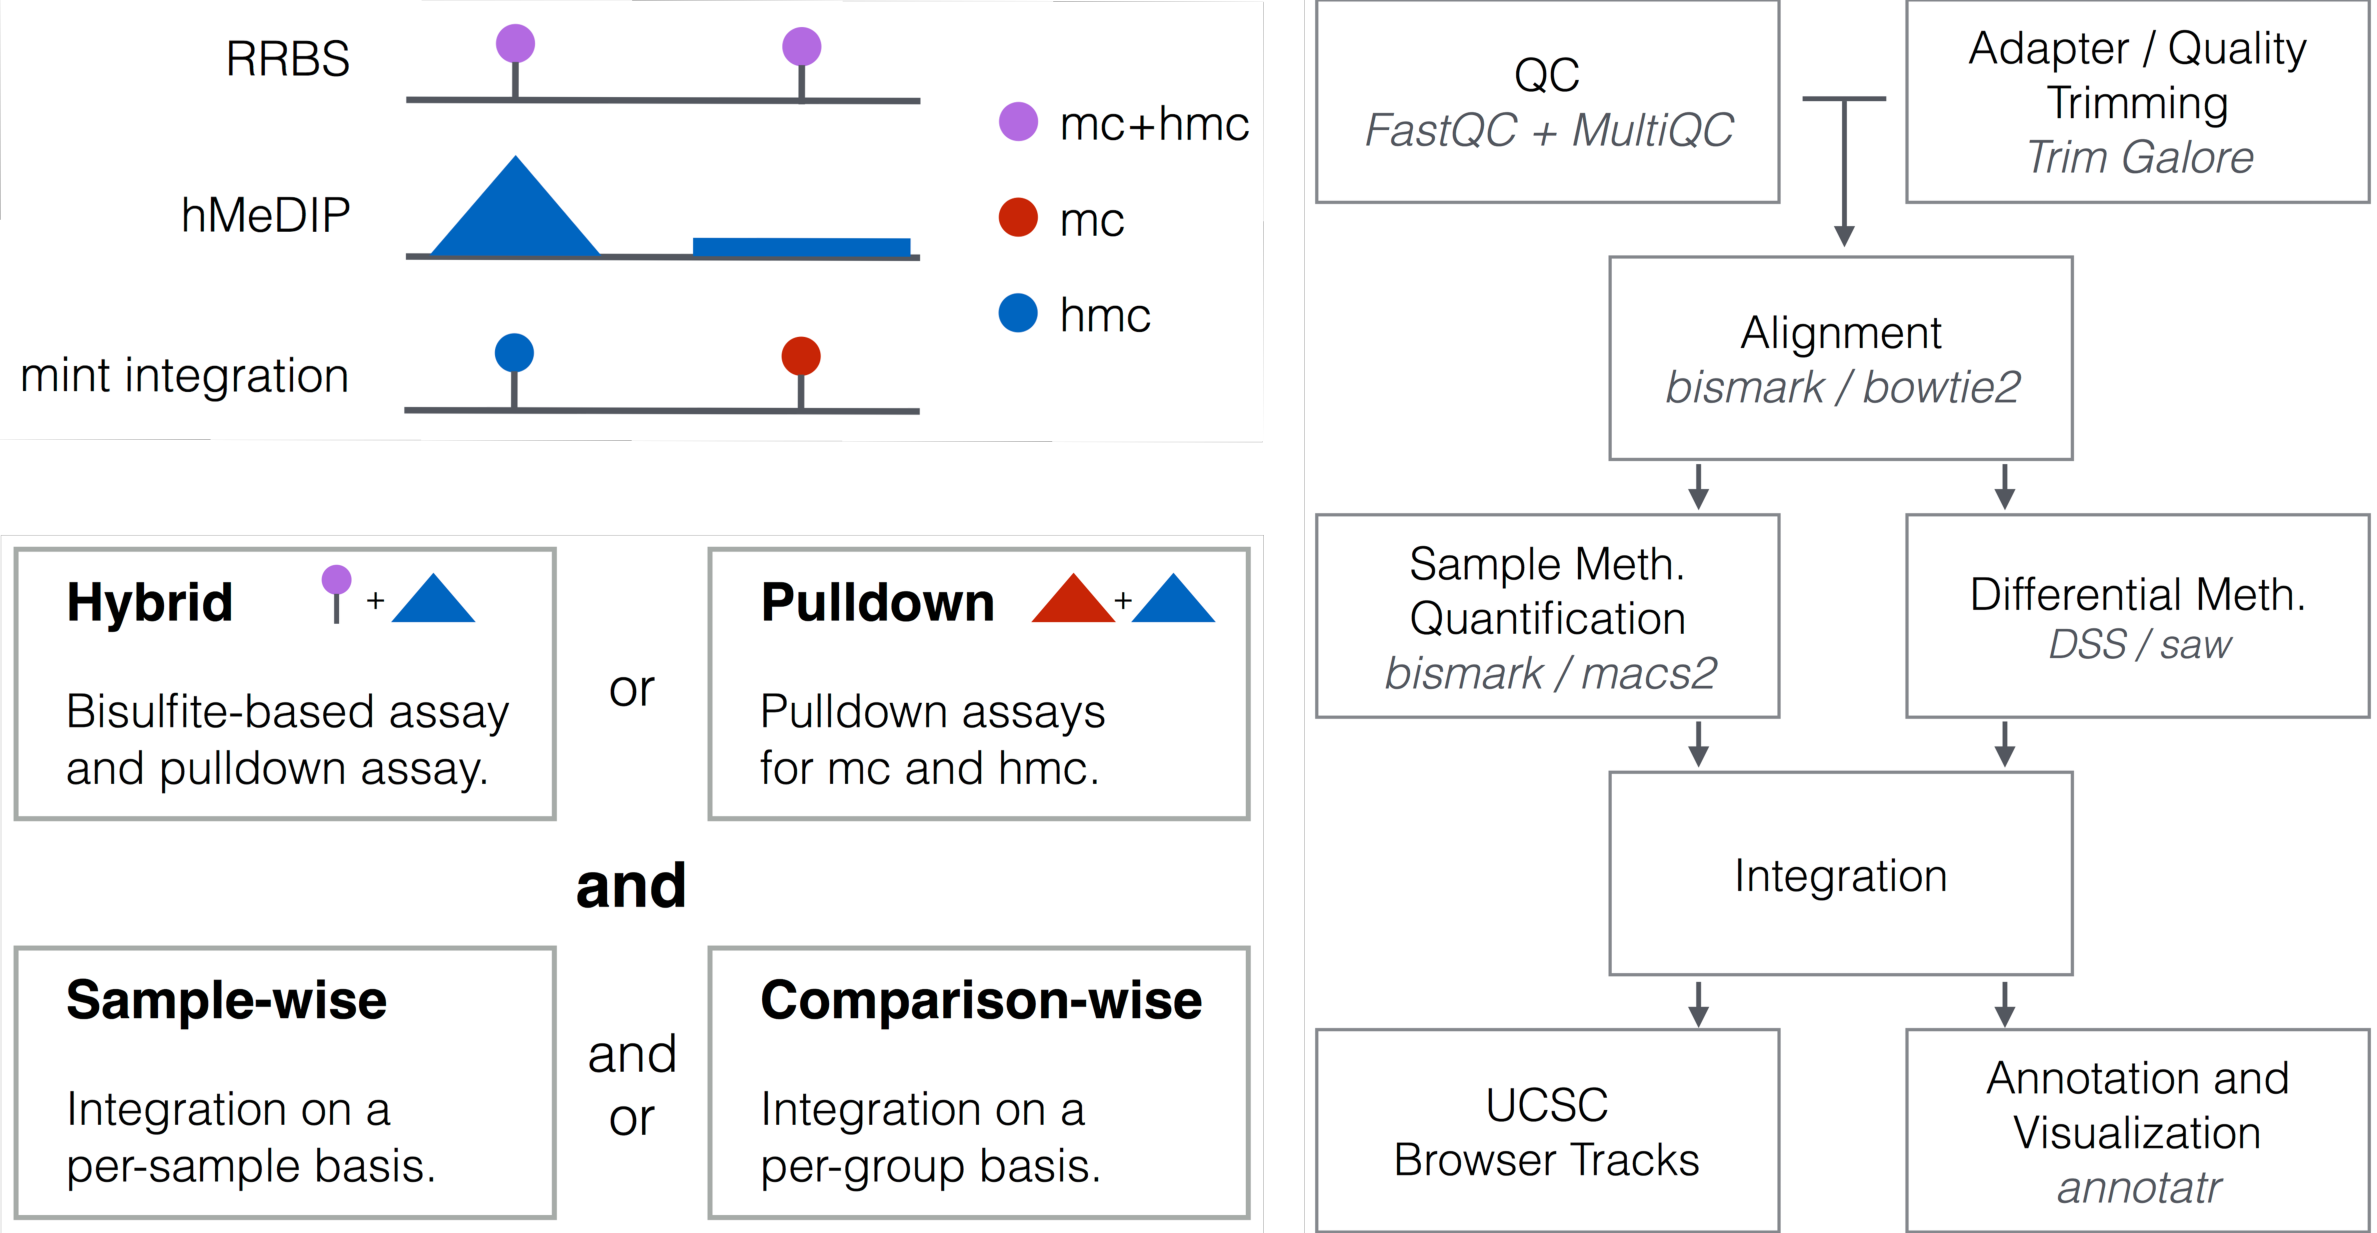
\includegraphics[width=1\textwidth]{chap5figs/figure5_1.pdf}
\caption[Conceptual overview of mint and implementation.]
{
% Rackham requires the figure list title matches the first sentence, so repeat that sentence here
\textbf{Conceptual overview of mint and implementation.} The concept behind 5mC and 5hmC integration. A summary of supported experimental setups and analyses. The overall mint workflow, with the primary tools used in each module.
}
\label{chap5:fig:1}
\end{figure}

\newpage

\begin{figure}[ht!]
\centering
% manually adjust the width of the figure
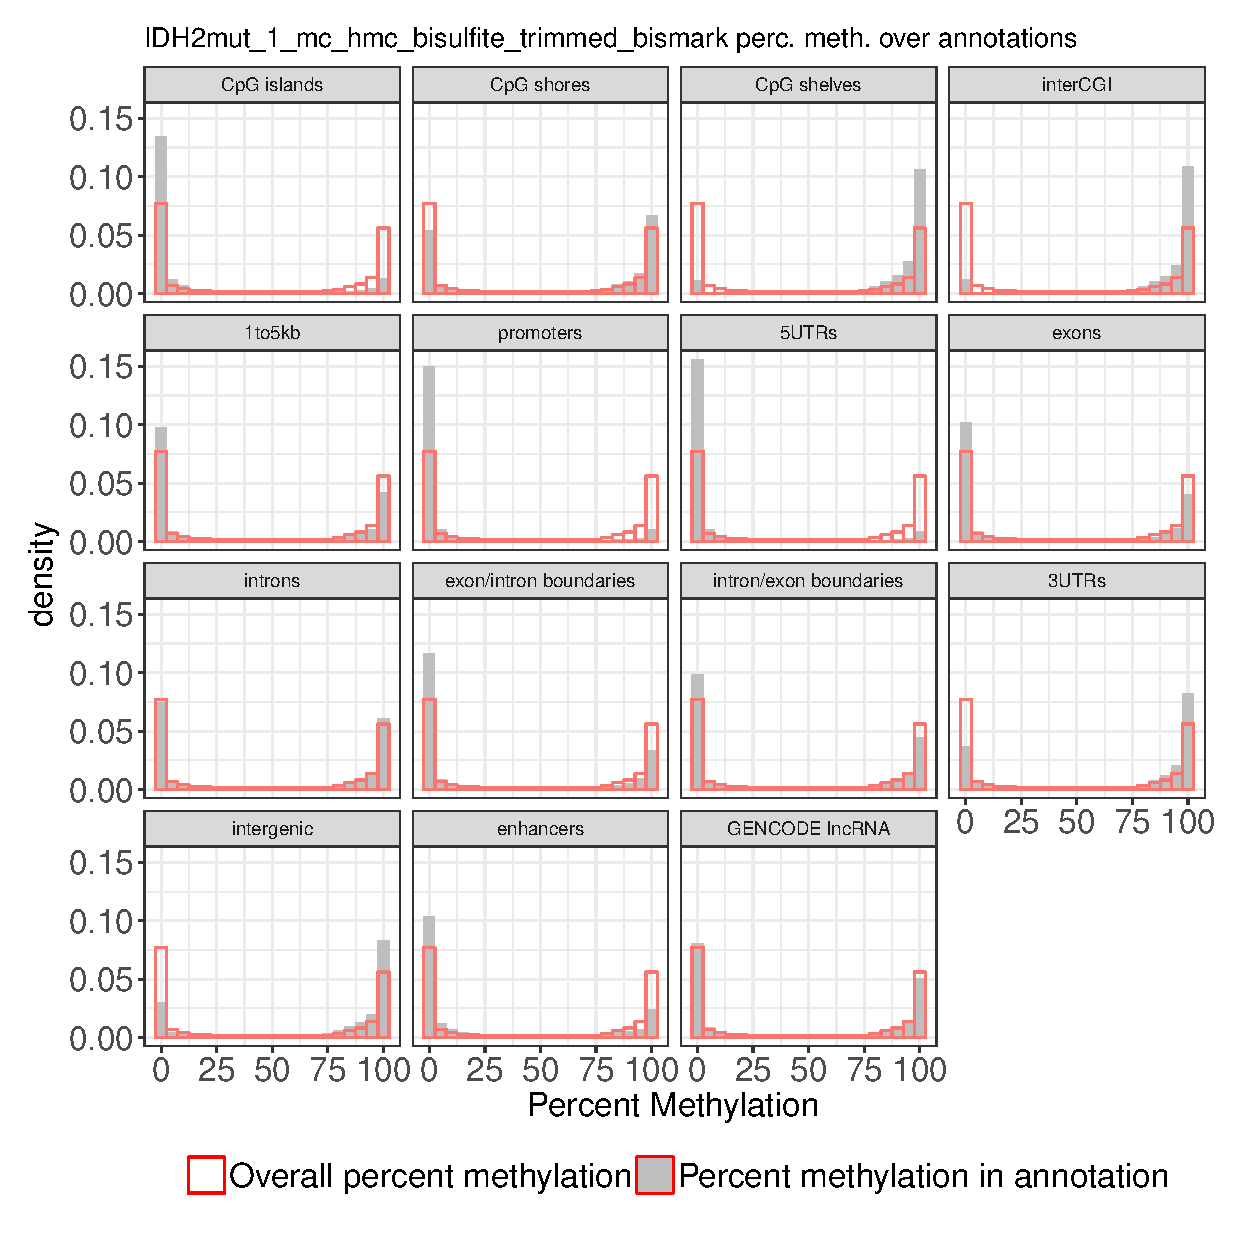
\includegraphics[width=1\textwidth]{chap5figs/figure5_2.eps}
\caption[The percent methylation in annotations from sample RRBS data.]
{
% Rackham requires the figure list title matches the first sentence, so repeat that sentence here
\textbf{The percent methylation in annotations from sample RRBS data.}
}
\label{chap5:fig:2}
\end{figure}

\newpage

\begin{figure}[ht!]
\centering
% manually adjust the width of the figure
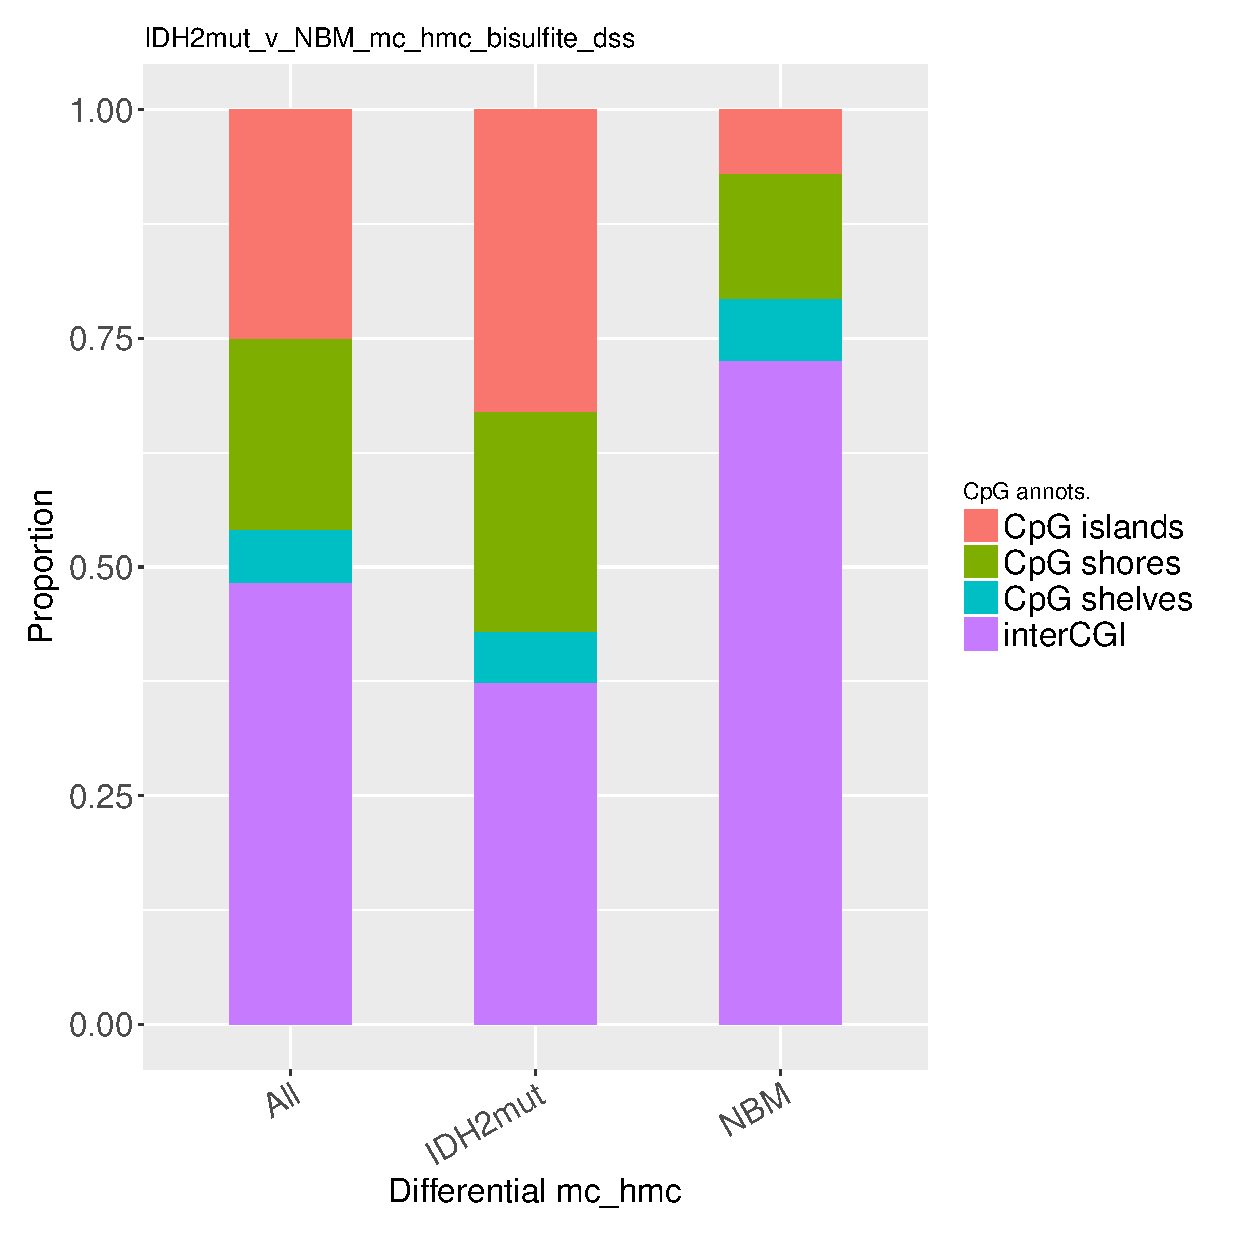
\includegraphics[width=1\textwidth]{chap5figs/figure5_3.eps}
\caption[The distribution of DhMRs from hMeSeal in CpG features.]
{
% Rackham requires the figure list title matches the first sentence, so repeat that sentence here
\textbf{The distribution of DhMRs from hMeSeal in CpG features.}
}
\label{chap5:fig:3}
\end{figure}

\newpage

\begin{figure}[ht!]
\centering
% manually adjust the width of the figure
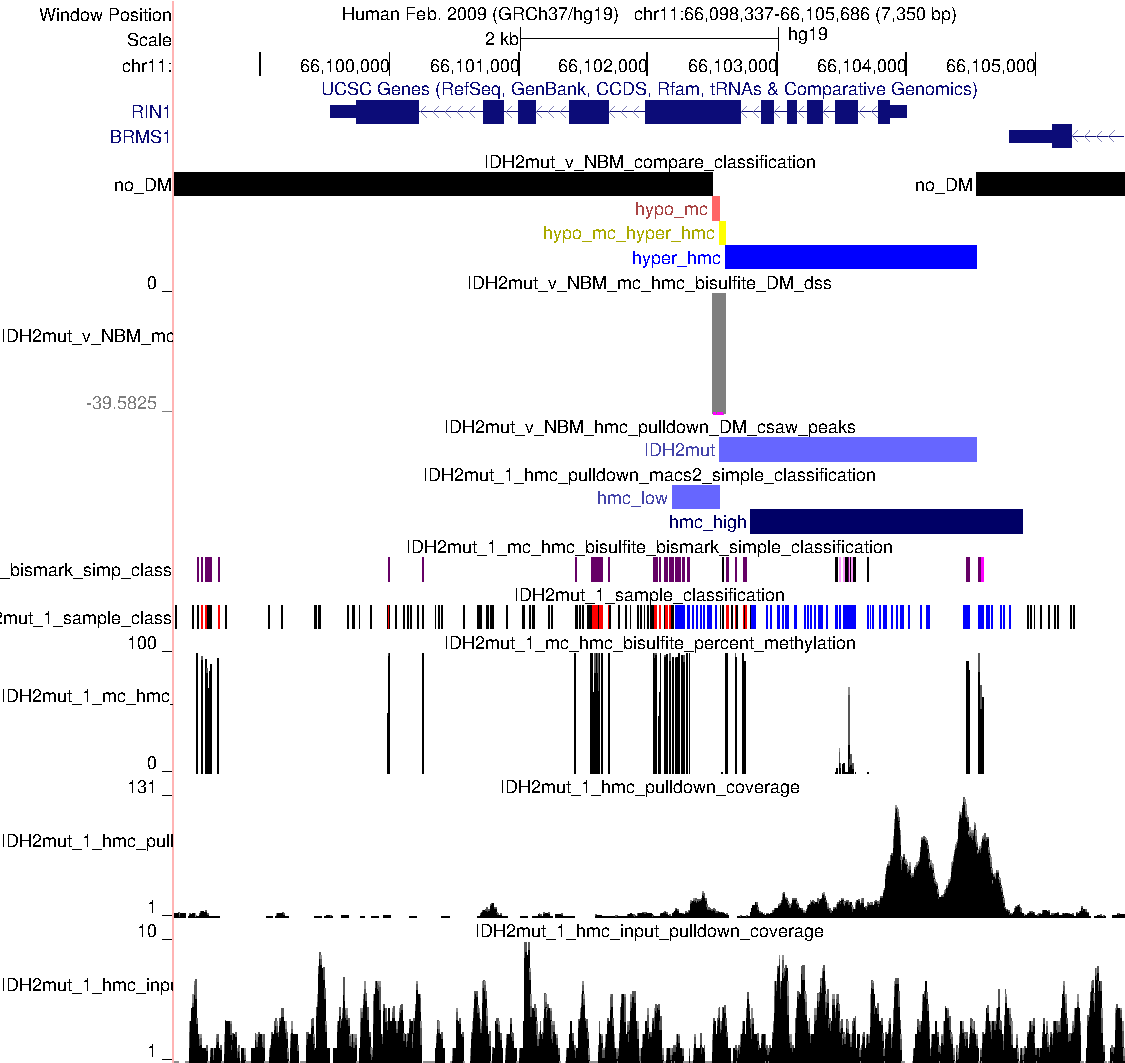
\includegraphics[width=1\textwidth]{chap5figs/figure5_4.pdf}
\caption[Example of UCSC Genome Browser tracks.]
{
% Rackham requires the figure list title matches the first sentence, so repeat that sentence here
\textbf{Example of UCSC Genome Browser tracks.} The RIN1 locus showing coordinated hypo 5mC and hyper 5hmC (yellow) in an internal exon and hyper 5hmC at the 5' end (blue).
}
\label{chap5:fig:4}
\end{figure}

\newpage

\begin{figure}[ht!]
\centering
% manually adjust the width of the figure
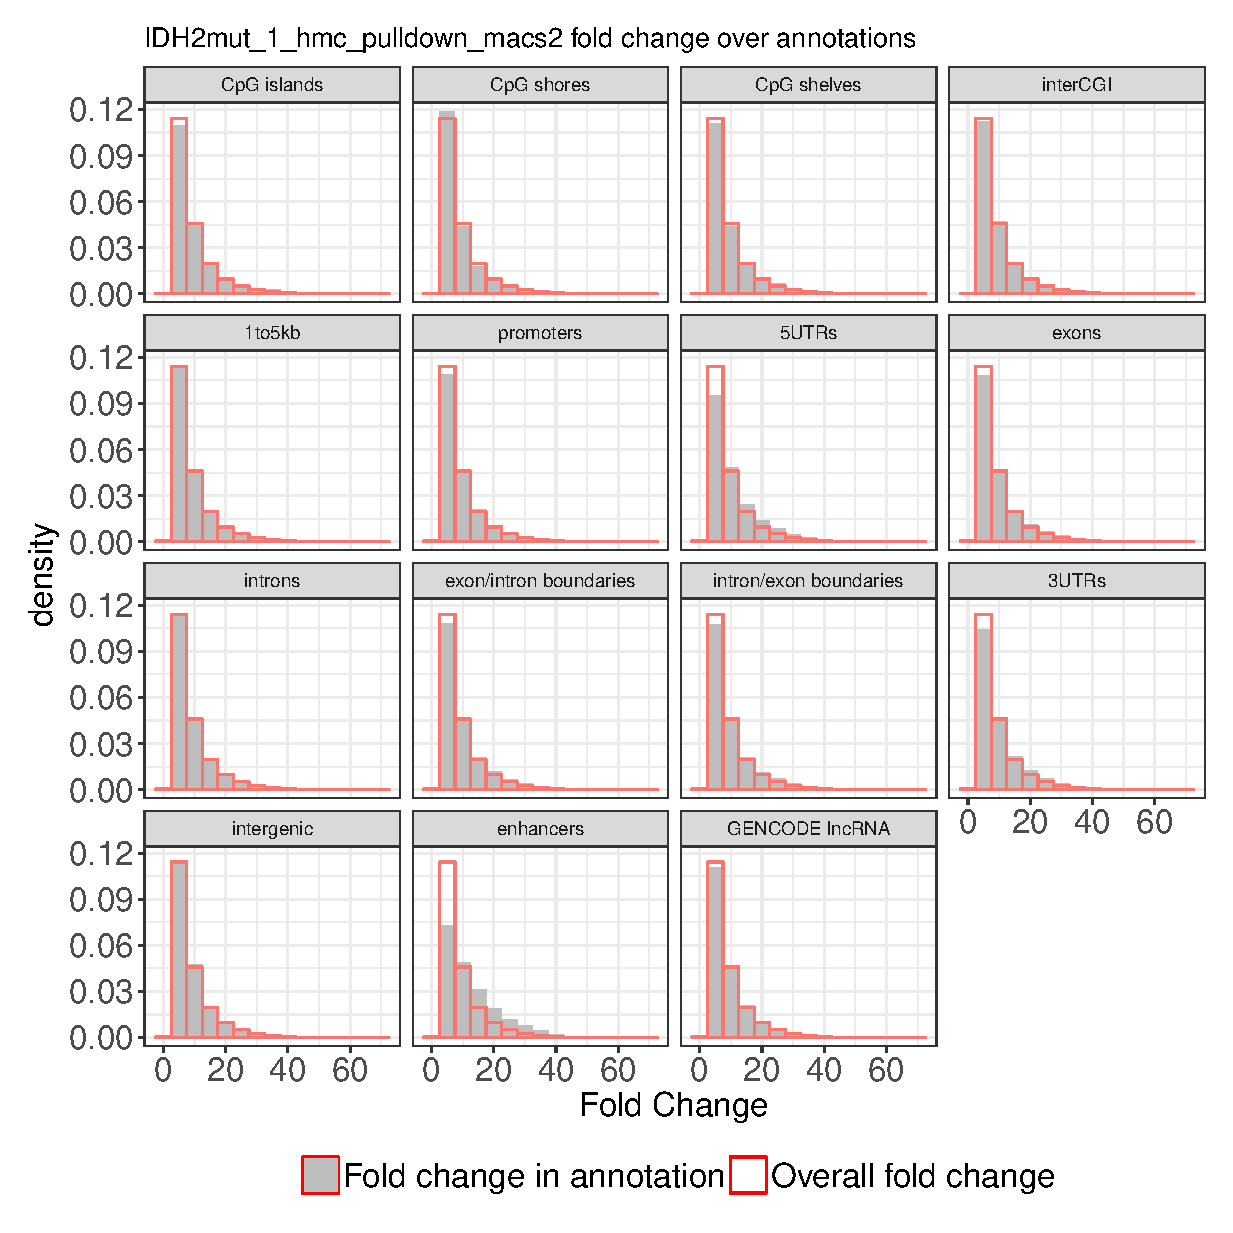
\includegraphics[width=1\textwidth]{chap5figs/figure5_5.eps}
\caption[Fold change of macs2 peaks measuring hydroxymethylation across genomic annotations.]
{
% Rackham requires the figure list title matches the first sentence, so repeat that sentence here
\textbf{Fold change of macs2 peaks measuring hydroxymethylation across genomic annotations.} Gray bars denote the fold change distribution for peaks annotated to the feature labeling the facet, and red outlines are the overall distribution of peak fold changes. Of note is the hyper-hydroxymethylation present in peaks annotated to enhancers and 5'UTRs compared to background.
}
\label{chap5:fig:5}
\end{figure}

\newpage

\begin{figure}[ht!]
\centering
% manually adjust the width of the figure
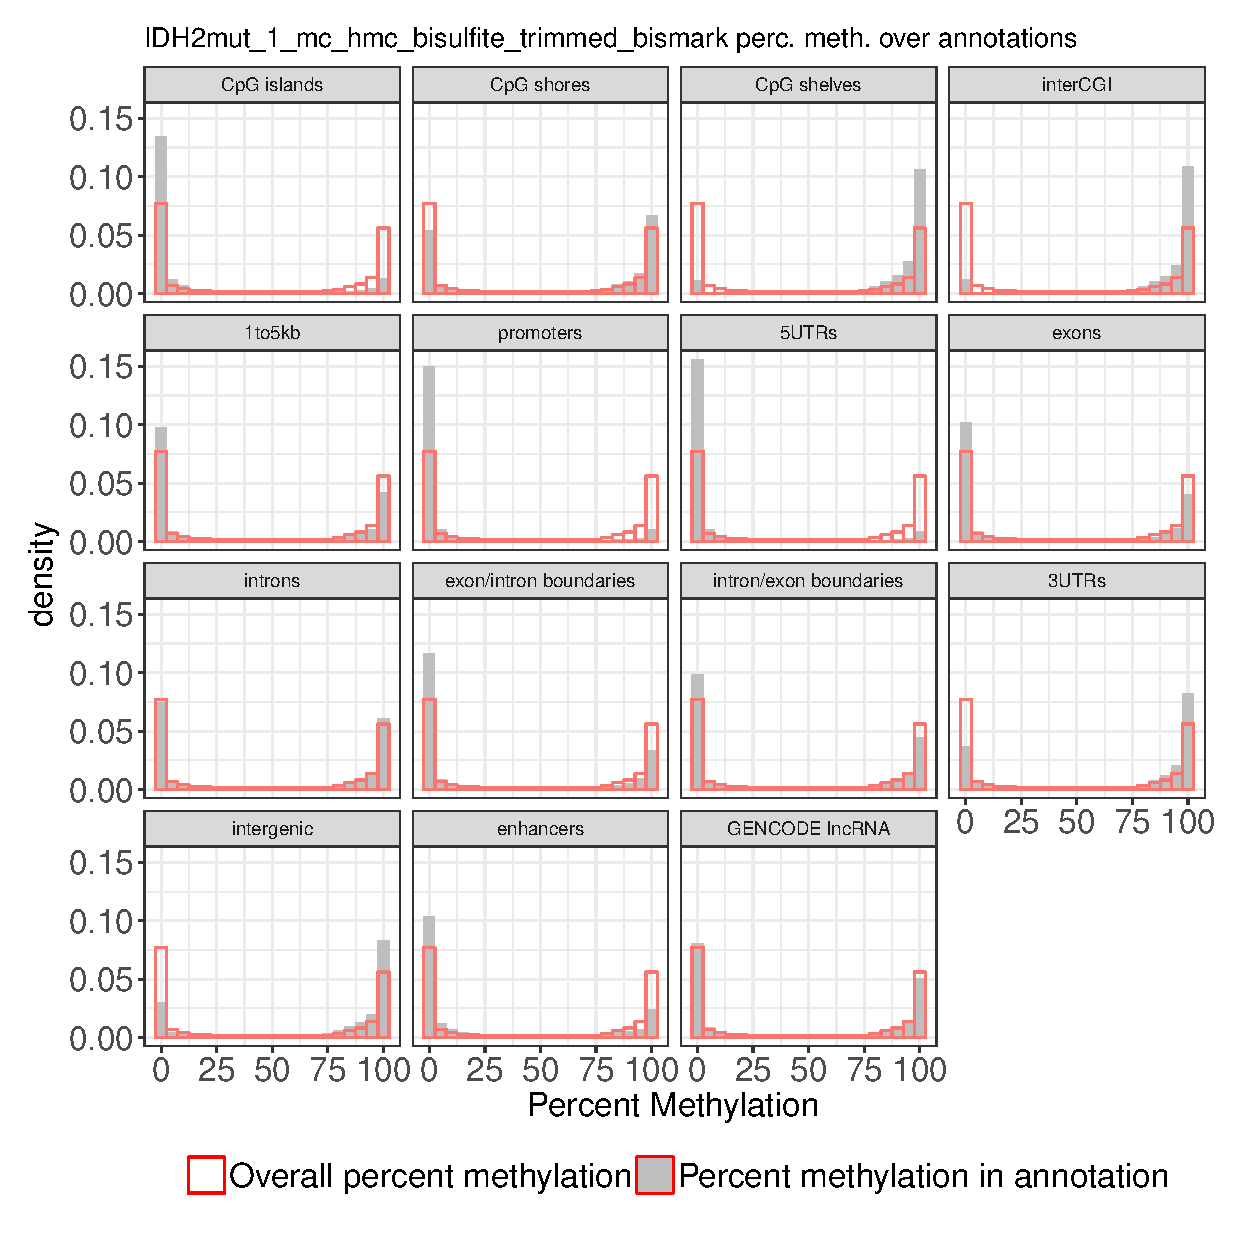
\includegraphics[width=1\textwidth]{chap5figs/figure5_6.eps}
\caption[Percent methylation of CpGs across genomic annotations.]
{
% Rackham requires the figure list title matches the first sentence, so repeat that sentence here
\textbf{Percent methylation of CpGs across genomic annotations.} Gray bars and red outlines are as in panel A. Of note is the hypo-methylation of CpGs annotated to enhancers and 5'UTRs relative to background, especially in light of corresponding hyper-hydroxymethylation.
}
\label{chap5:fig:6}
\end{figure}

\newpage

\begin{figure}[ht!]
\centering
% manually adjust the width of the figure
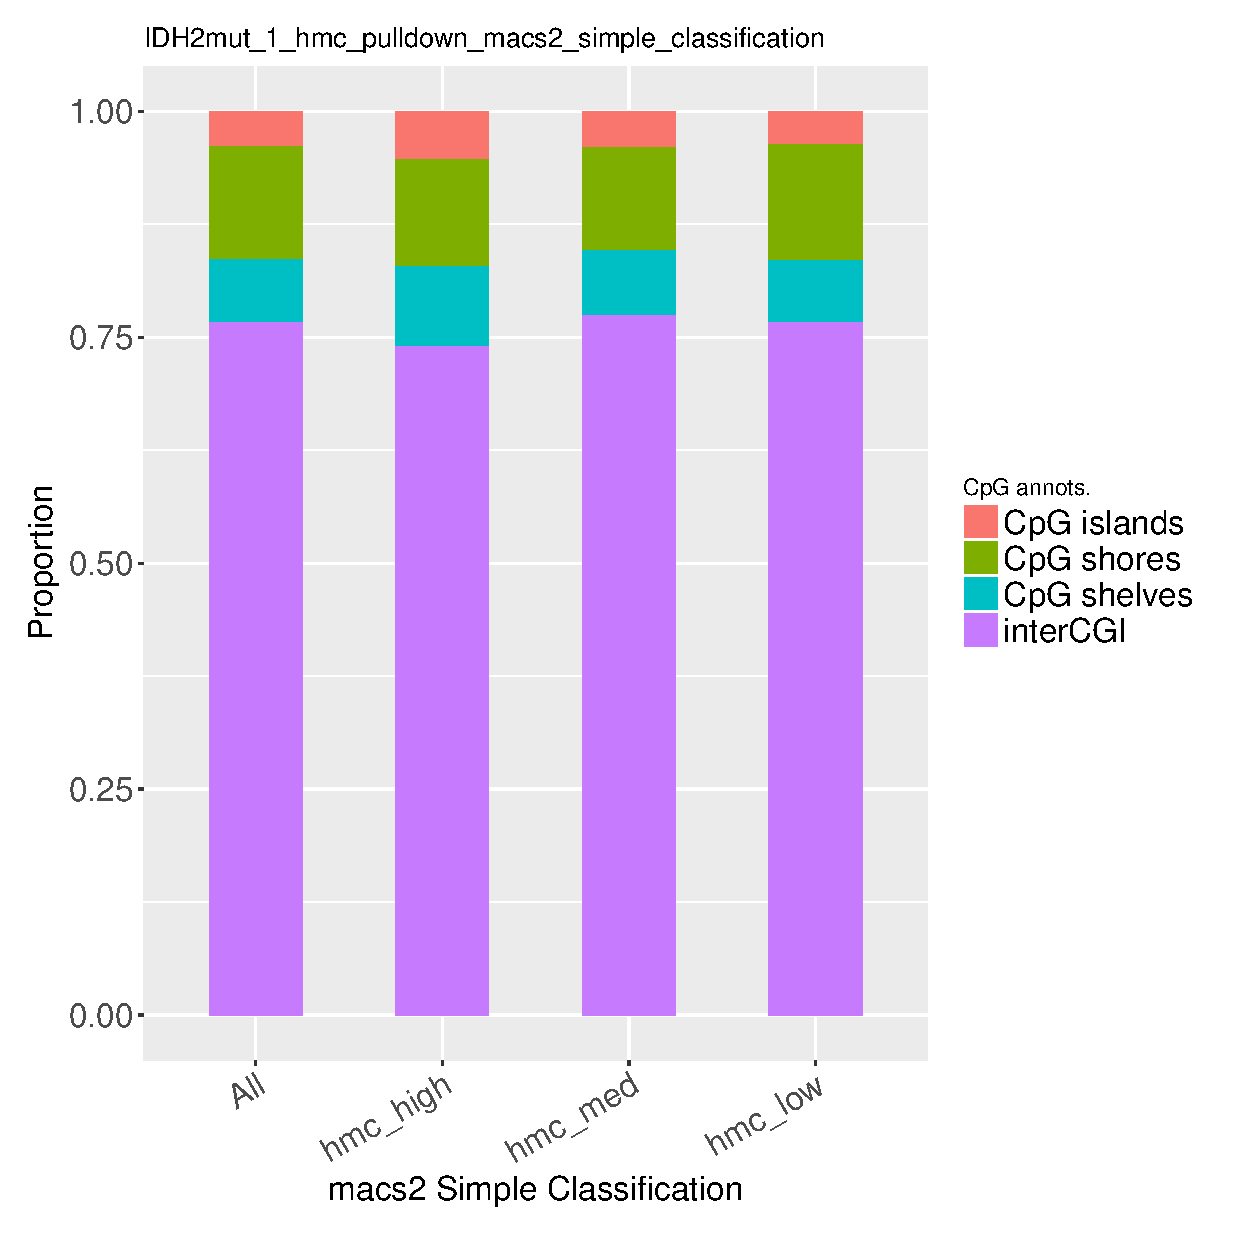
\includegraphics[width=1\textwidth]{chap5figs/figure5_7.eps}
\caption[Annotations of the simple classification across CpG features.]
{
% Rackham requires the figure list title matches the first sentence, so repeat that sentence here
\textbf{Annotations of the simple classification for hydroxymethylation across CpG features.} Classifications of hydroxymethylation are similarly distributed across CpG features regardless of peak strength.
}
\label{chap5:fig:7}
\end{figure}

\newpage

\begin{figure}[ht!]
\centering
% manually adjust the width of the figure
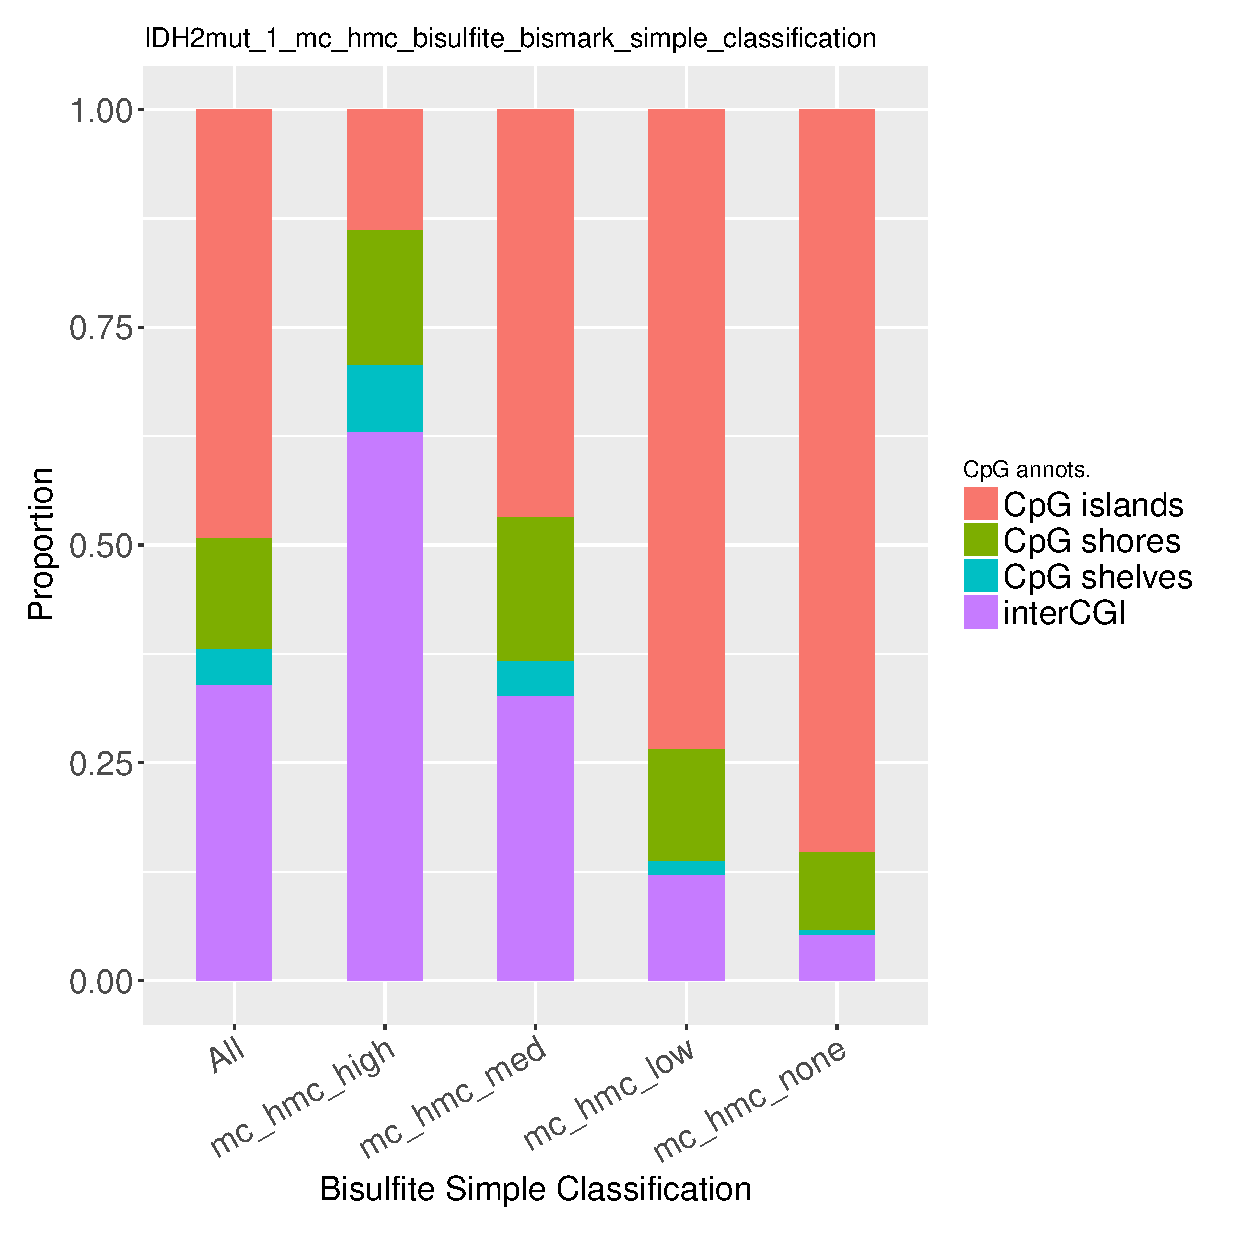
\includegraphics[width=1\textwidth]{chap5figs/figure5_8.eps}
\caption[Annotations of the simple classification.]
{
% Rackham requires the figure list title matches the first sentence, so repeat that sentence here
\textbf{Annotations of the simple classification for methylation across CpG features.} CpGs have different distributions across CpG features according to strength of methylation. In particular, as methylation weakens, it tends to be located more in CpG islands (orange), but less in CpG shelves (blue).
}
\label{chap5:fig:8}
\end{figure}

\newpage

\begin{figure}[ht!]
\centering
% manually adjust the width of the figure
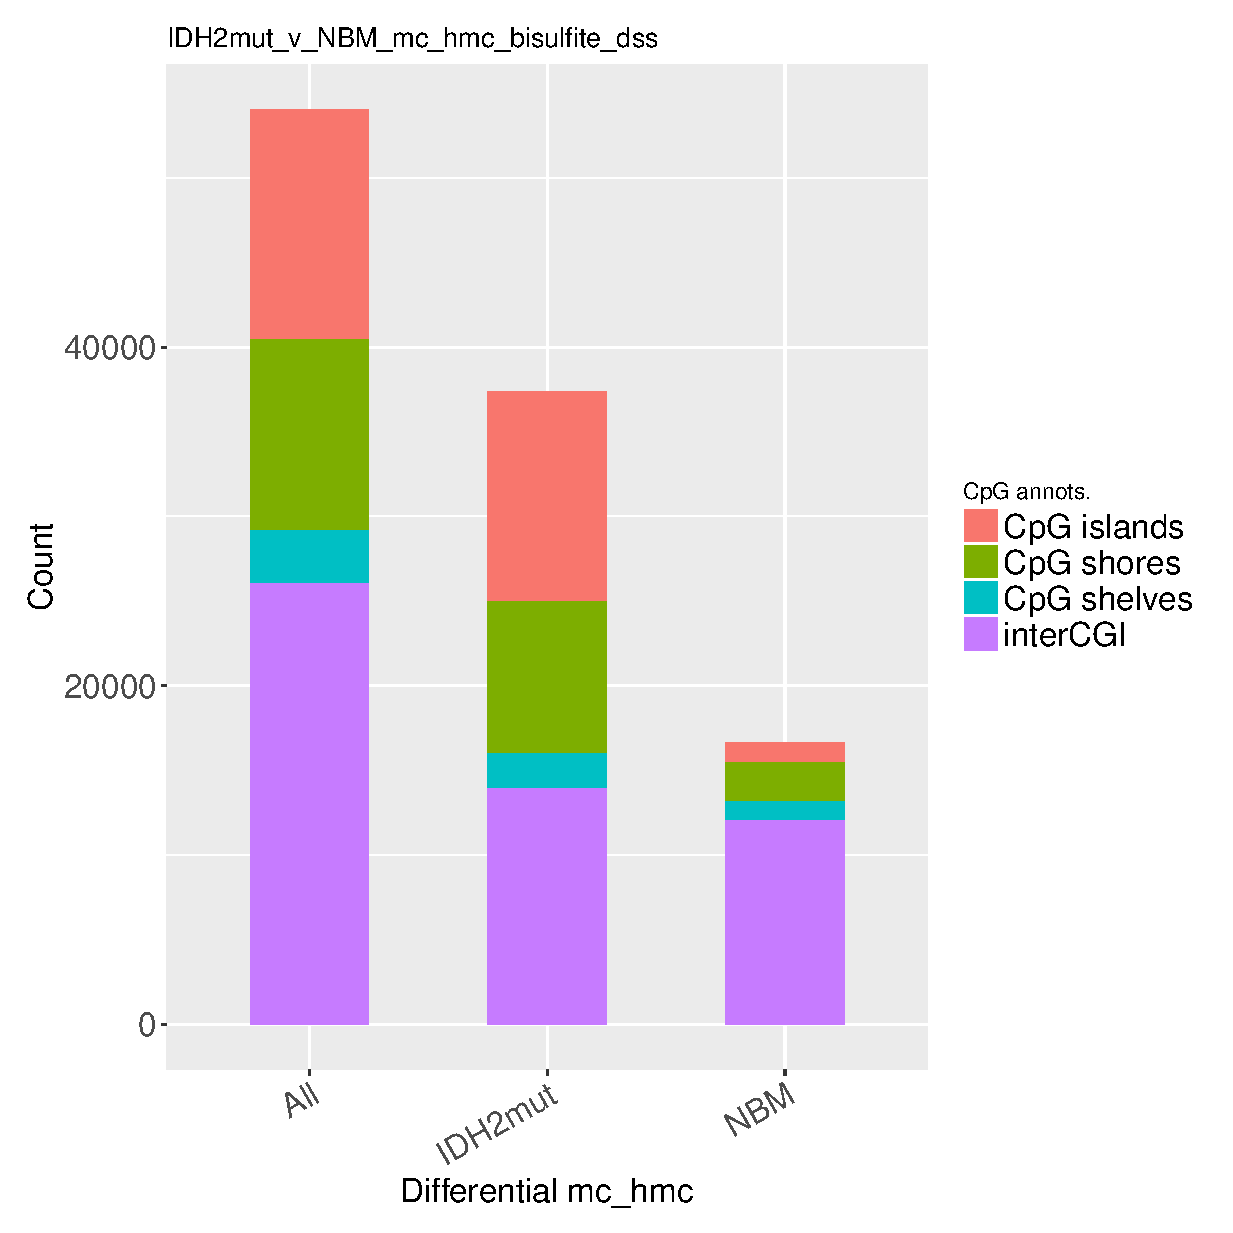
\includegraphics[width=1\textwidth]{chap5figs/figure5_9.eps}
\caption[Number of DMRs found by DSS, and annotated to CpG island features.]
{
% Rackham requires the figure list title matches the first sentence, so repeat that sentence here
\textbf{Number of DMRs found by DSS, and annotated to CpG island features.} The number of hyper-methylated DMRs in the IDH2 samples is greater than those in NBM samples, in line with previous findings.
}
\label{chap5:fig:9}
\end{figure}

\newpage

\begin{figure}[ht!]
\centering
% manually adjust the width of the figure
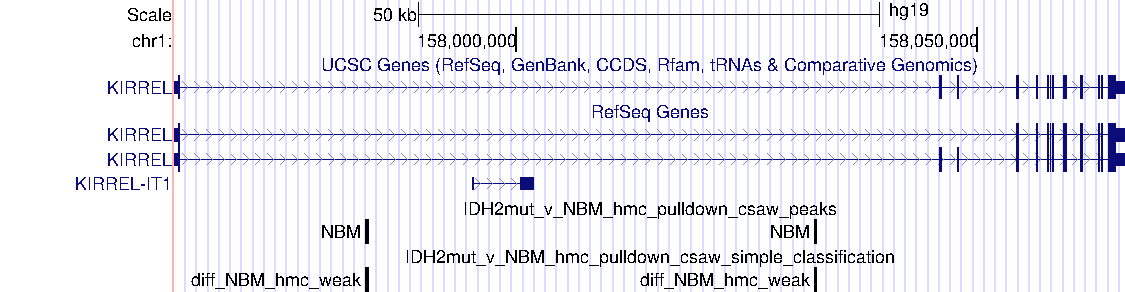
\includegraphics[width=1\textwidth]{chap5figs/figure5_10.pdf}
\caption[DhMRs at the KIRREL locus.]
{
% Rackham requires the figure list title matches the first sentence, so repeat that sentence here
\textbf{DhMRs at the KIRREL locus.} The Genome Browser with csaw track showing 'NBM' peaks (hypo-hydroxymethylated in IDH2 mutants) as was found in the paper originally describing the AML data.
}
\label{chap5:fig:10}
\end{figure}

\newpage

\begin{figure}[ht!]
\centering
% manually adjust the width of the figure
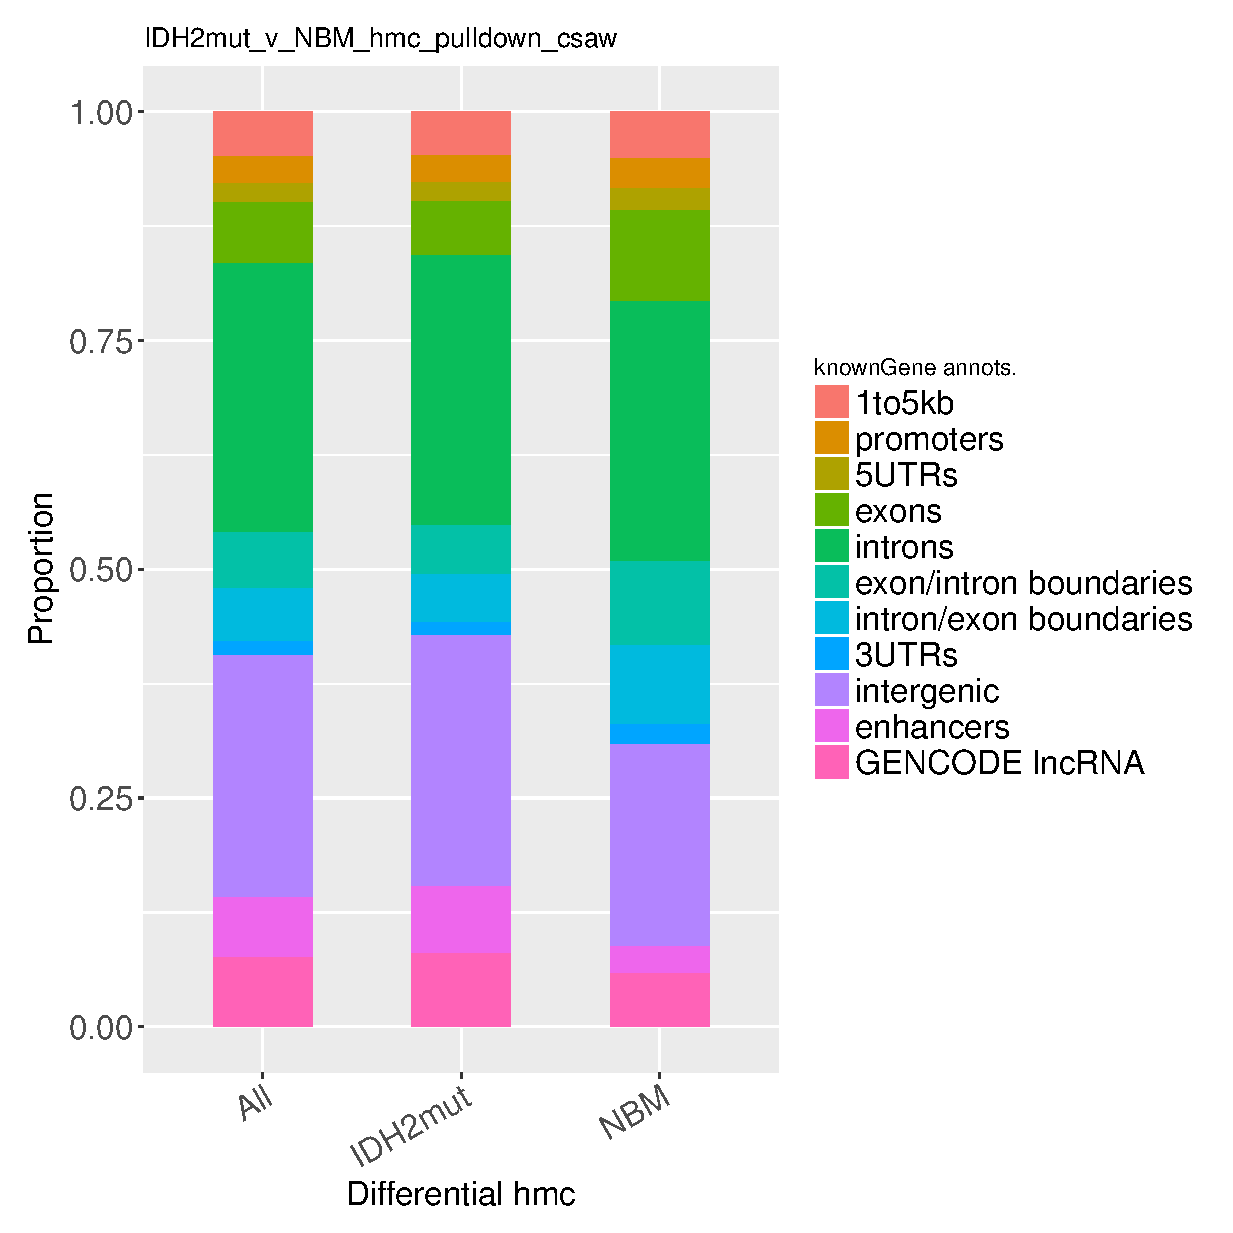
\includegraphics[width=1\textwidth]{chap5figs/figure5_11.eps}
\caption[DhMRs at genic annotations.]
{
% Rackham requires the figure list title matches the first sentence, so repeat that sentence here
\textbf{DhMRs at genic annotations.} Hypo-hydroxymethylated regions in IDH2 mutants occur more frequently at 5' ends of genes and exons than hyper-hydroxymethylated regions.
}
\label{chap5:fig:11}
\end{figure}

\newpage

\begin{figure}[ht!]
\centering
% manually adjust the width of the figure
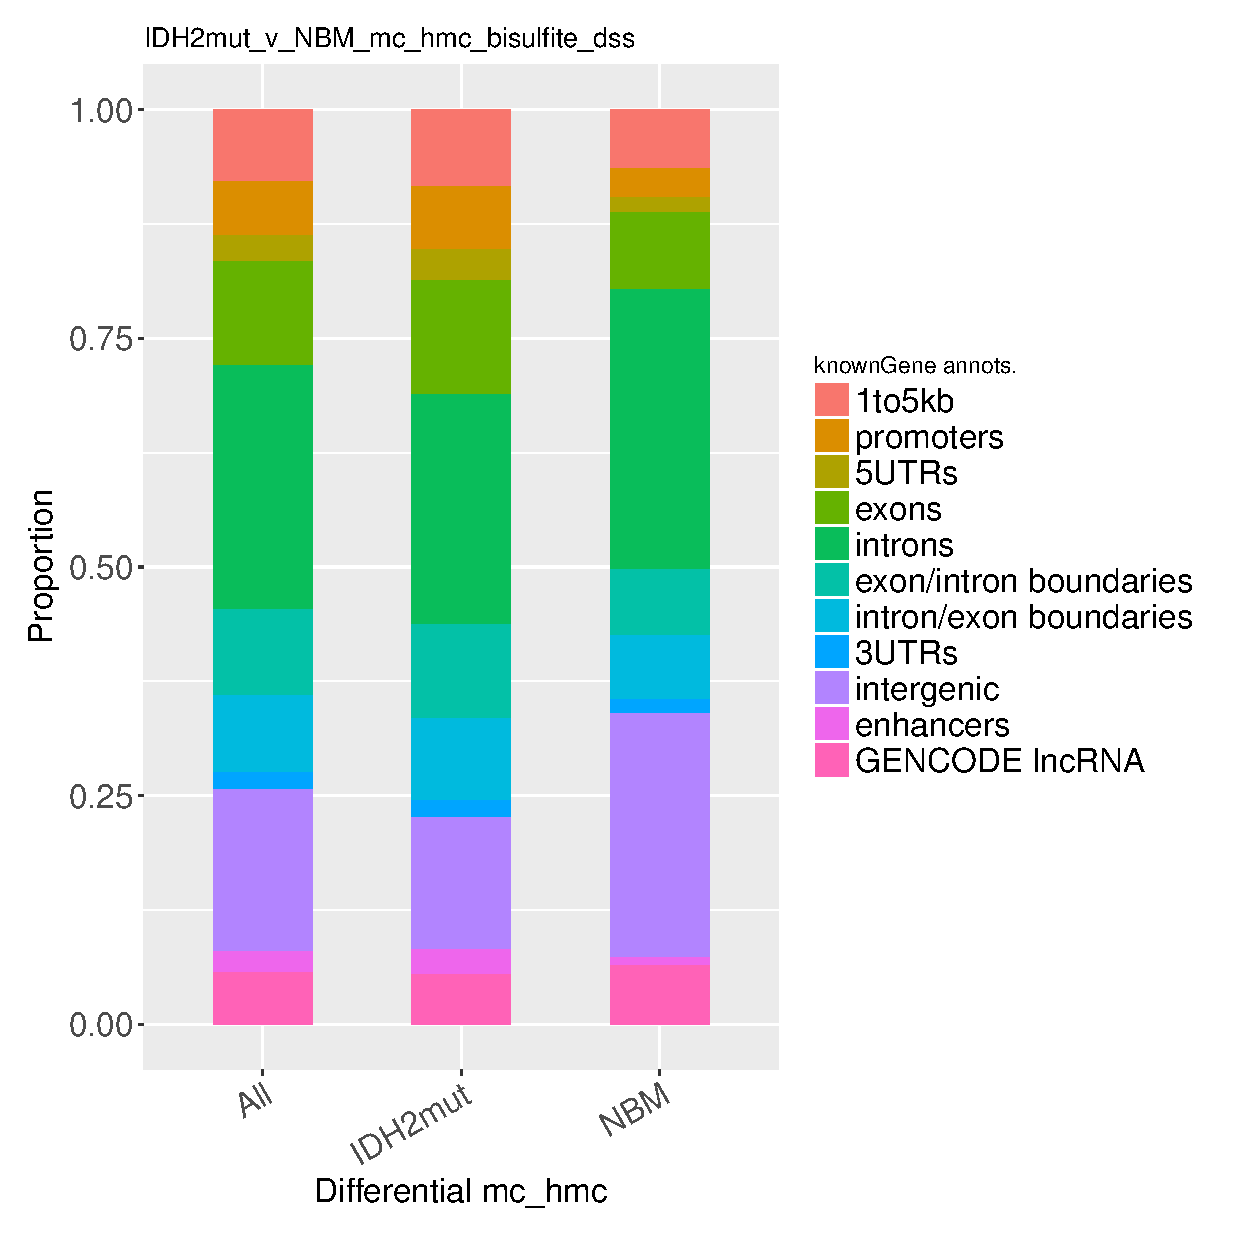
\includegraphics[width=1\textwidth]{chap5figs/figure5_12.eps}
\caption[DMRs at genic annotations.]
{
% Rackham requires the figure list title matches the first sentence, so repeat that sentence here
\textbf{DMRs at genic annotations.} Hyper-methylated regions in IDH2 mutants occur more frequently at 5' ends of genes and exons than hypo-methylated regions.
}
\label{chap5:fig:12}
\end{figure}

\newpage

\begin{figure}[ht!]
\centering
% manually adjust the width of the figure
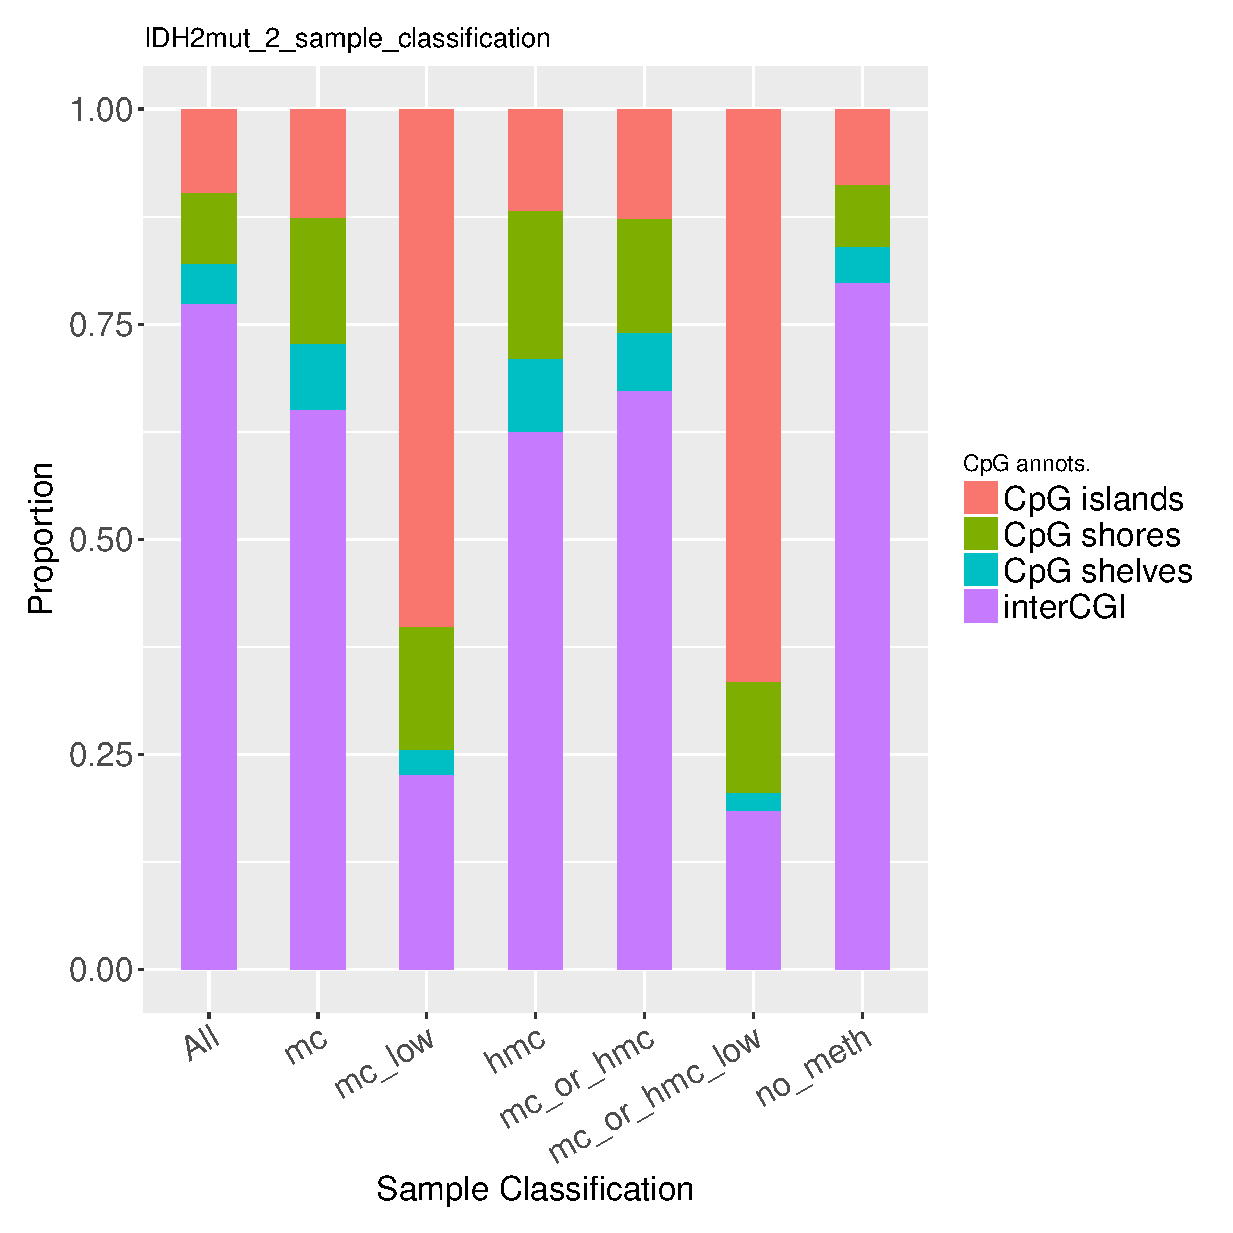
\includegraphics[width=1\textwidth]{chap5figs/figure5_14.eps}
\caption[Genomic annotation to CpG features for sample-wise classification of 5mC and 5hmC signals.]
{
% Rackham requires the figure list title matches the first sentence, so repeat that sentence here
\textbf{Genomic annotation to CpG features for sample-wise classification of 5mC and 5hmC signals.} In the IDH2mut\_2 sample, combined 5mC (mc and mc\_low) classifications occur more frequently in CpG islands (orange) than 5hmC.
}
\label{chap5:fig:14}
\end{figure}

\newpage

\begin{figure}[ht!]
\centering
% manually adjust the width of the figure
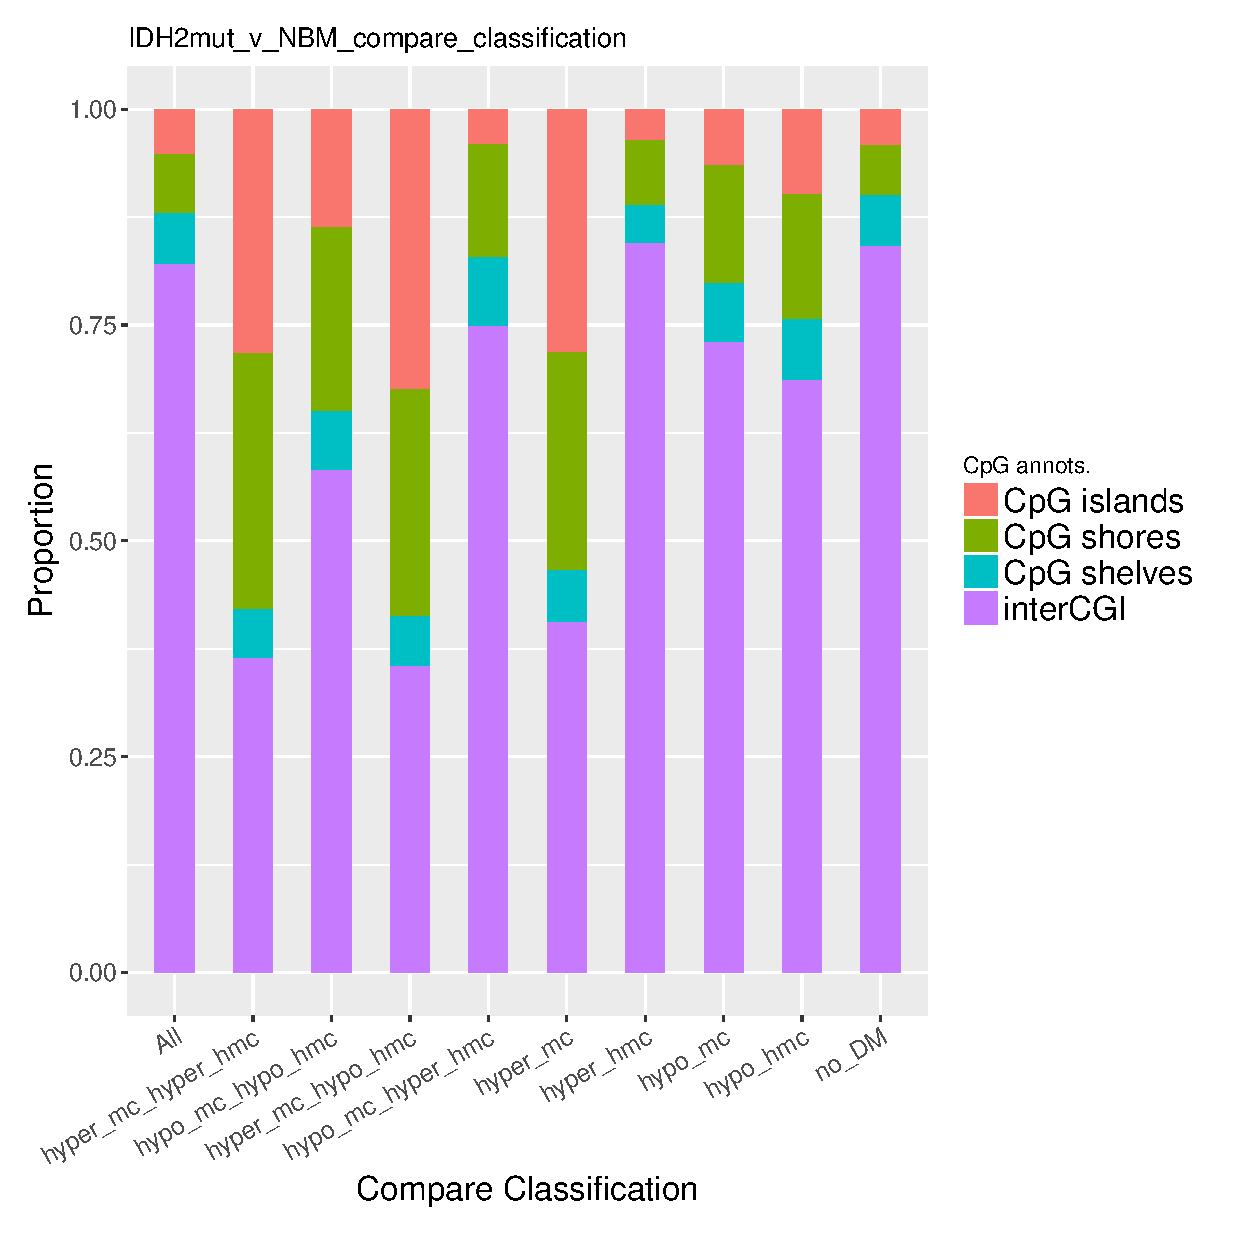
\includegraphics[width=1\textwidth]{chap5figs/figure5_15.eps}
\caption[Genomic annotation to CpG features of DhMR and DMR signal in the comparison of IDH2 mutant to NBM samples.]
{
% Rackham requires the figure list title matches the first sentence, so repeat that sentence here
\textbf{Genomic annotation to CpG features of DhMR and DMR signal in the comparison of IDH2 mutant to NBM samples.}
}
\label{chap5:fig:15}
\end{figure}

\newpage

\begin{figure}[ht!]
\centering
% manually adjust the width of the figure
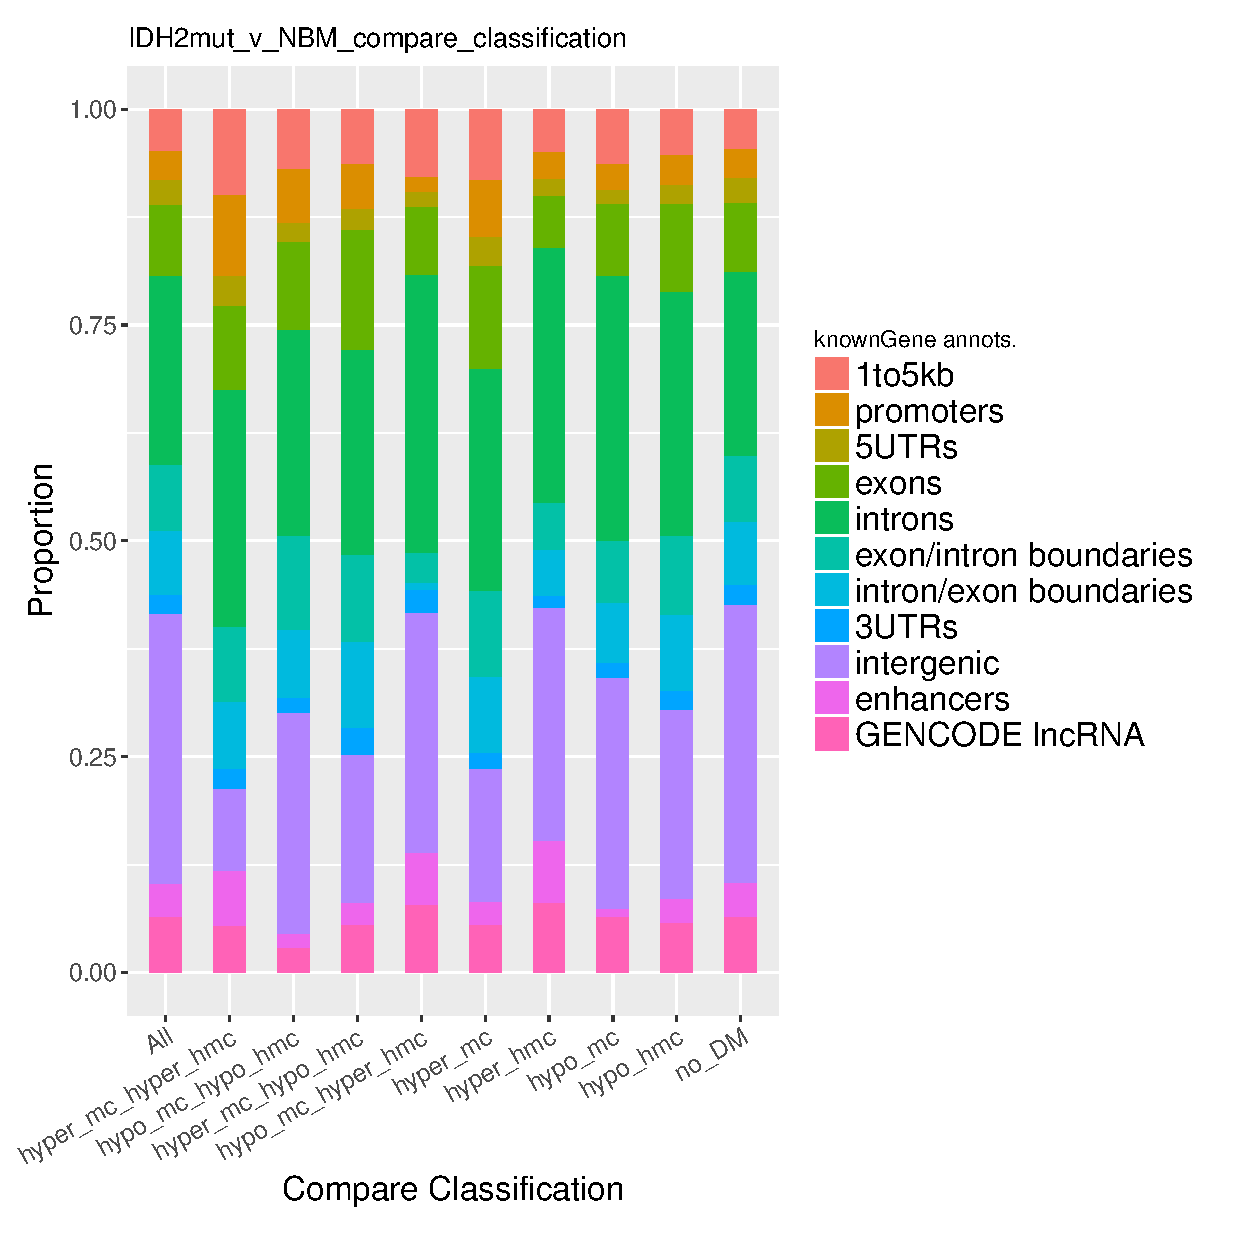
\includegraphics[width=1\textwidth]{chap5figs/figure5_16.eps}
\caption[Genomic annotation to genic features, enhancers, and GENCODE lncRNA of DhMR and DMR signal in the comparison of IDH2 mutant to NBM samples.]
{
% Rackham requires the figure list title matches the first sentence, so repeat that sentence here
\textbf{Genomic annotation to genic features, enhancers, and GENCODE lncRNA of DhMR and DMR signal in the comparison of IDH2 mutant to NBM samples.}
}
\label{chap5:fig:16}
\end{figure}

\newpage

\begin{figure}[ht!]
\centering
% manually adjust the width of the figure
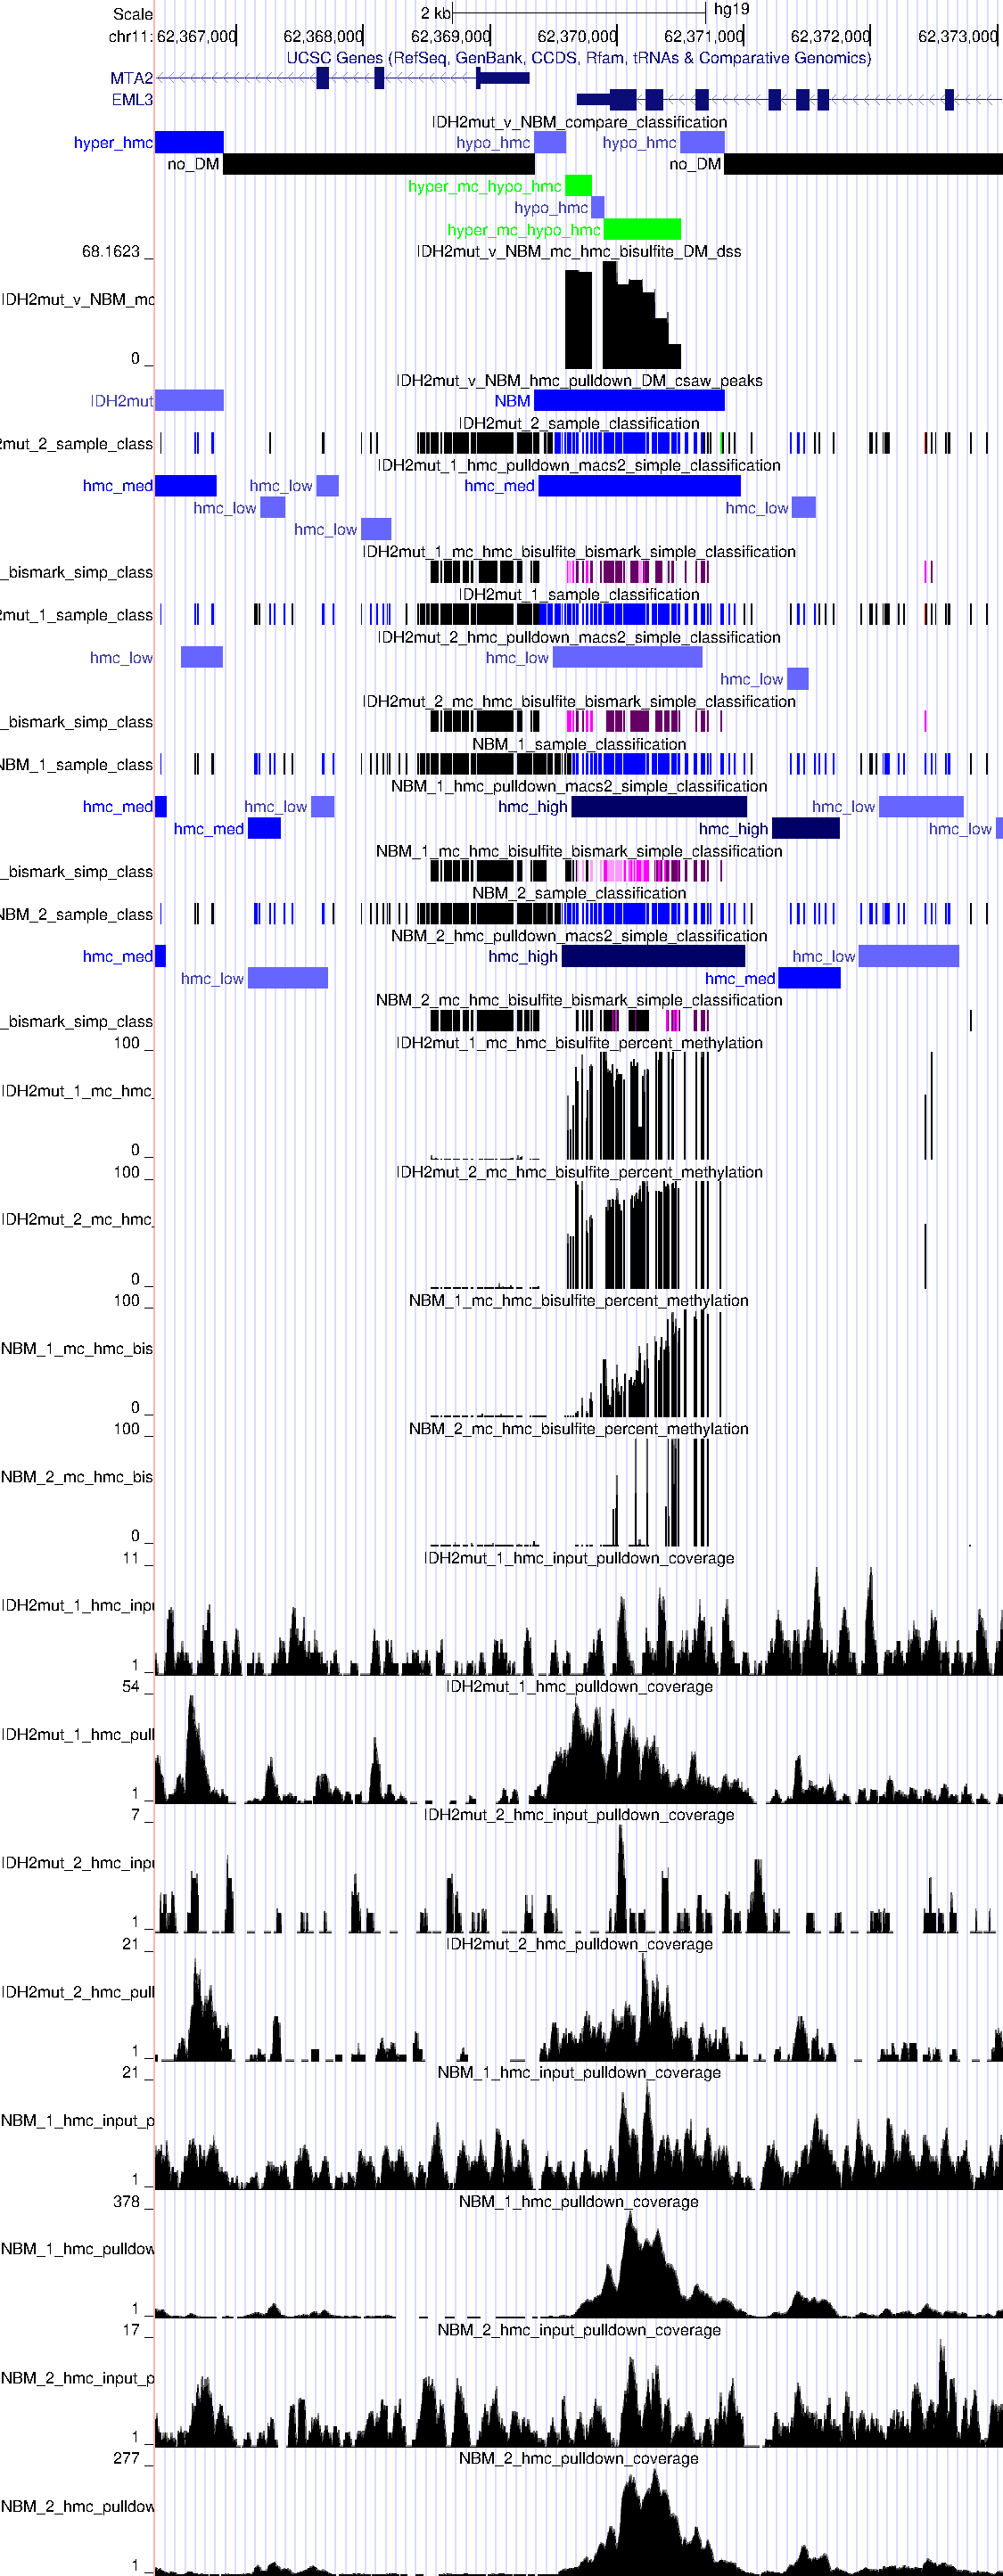
\includegraphics[width=0.5\textwidth]{chap5figs/figure5_17.pdf}
\caption[A display of the entire UCSC Genome Browser track hub.]
{
% Rackham requires the figure list title matches the first sentence, so repeat that sentence here
\textbf{A display of the entire UCSC Genome Browser track hub.} All tracks from the track hub are displayed for the a genomic region containing MTA2 and EML3, which shows simultaneous hypo-hydroxymethylation and hyper-methylation in IDH2 mutants. Tracks have a default grouping based on the track type, but are easily rearranged by the user. For example, the track from the compare\_classification module is grouped with the csaw and DSS tracks since the classification track is the intersection of the latter two.
}
\label{chap5:fig:17}
\end{figure}

\clearpage
\section*{Tables}
\begin{sidewaystable}[!ht]
\small
\centering
\begin{tabular}{lllllllllll}
\textbf{projectID} & \textbf{sampleID}          & \textbf{humanID} & \textbf{pulldown} & \textbf{bisulfite} & \textbf{mc} & \textbf{hmc} & \textbf{input} & \textbf{group} & \textbf{subject} & \textbf{age} \\
test\_hybrid       & IDH2mut\_1\_hmeseal        & IDH2mut\_1       & 1                 & 0                  & 0           & 1            & 0              & 1              & 1                & 3            \\
test\_hybrid       & IDH2mut\_2\_hmeseal        & IDH2mut\_2       & 1                 & 0                  & 0           & 1            & 0              & 1              & 2                & 3            \\
test\_hybrid       & IDH2mut\_1\_hmeseal\_input & IDH2mut\_1       & 1                 & 0                  & 0           & 1            & 1              & 1              & 1                & 3            \\
test\_hybrid       & IDH2mut\_2\_hmeseal\_input & IDH2mut\_2       & 1                 & 0                  & 0           & 1            & 1              & 1              & 2                & 3            \\
test\_hybrid       & IDH2mut\_1\_errbs          & IDH2mut\_1       & 0                 & 1                  & 1           & 1            & 0              & 1              & 1                & 3            \\
test\_hybrid       & IDH2mut\_2\_errbs          & IDH2mut\_2       & 0                 & 1                  & 1           & 1            & 0              & 1              & 2                & 3            \\
test\_hybrid       & NBM\_1\_hmeseal            & NBM\_1           & 1                 & 0                  & 0           & 1            & 0              & 0              & 1                & 10           \\
test\_hybrid       & NBM\_2\_hmeseal            & NBM\_2           & 1                 & 0                  & 0           & 1            & 0              & 0              & 2                & 10           \\
test\_hybrid       & NBM\_1\_hmeseal\_input     & NBM\_1           & 1                 & 0                  & 0           & 1            & 1              & 0              & 1                & 10           \\
test\_hybrid       & NBM\_2\_hmeseal\_input     & NBM\_2           & 1                 & 0                  & 0           & 1            & 1              & 0              & 2                & 10           \\
test\_hybrid       & NBM\_1\_errbs              & NBM\_1           & 0                 & 1                  & 1           & 1            & 0              & 0              & 1                & 10           \\
test\_hybrid       & NBM\_2\_errbs              & NBM\_2           & 0                 & 1                  & 1           & 1            & 0              & 0              & 2                & 10
\end{tabular}
\normalsize
\caption[Example of sample metadata and covariate information to be used in setting up a mint project.]
{
% Rackham requires the figure list title matches the first sentence, so repeat that sentence here
\textbf{Example of sample metadata and covariate information to be used in setting up a mint project.}
The table should be tab-delimited and placed in the mint/projects folder with a filename of the form [projectID]\_samples.txt. This ensures that the init.R initialization script looks at the proper metadata table for the project. The sampleID column will often not be human readable (i.e. automatically named .fastq.gz files provided by a sequencing core, GEO, or SRA). The humanID column is meant to connect human understandable names to the automatically generated IDs. The pulldown, bisulfite, mc, hmc, and input columns are binary where 0 means no and 1 means yes. In the example below, any bisulfite sample has a 1 in the mc and hmc columns to indicate that the platform (in this case ERRBS) cannot distinguish between them. The group column can contain multiple comma-separated numbers if a sample belongs to more than one group (e.g. '1,2'). Columns appearing after the group column are considered covariates to be used in the models used for differential methylation testing with csaw and DSS. Column headers for covariate columns must match the variables as they appear in the model and covariate columns of the comparisons table (Table \ref{chap5:table:2}).
}
\label{chap5:table:1}

\end{sidewaystable}

\newpage

\begin{sidewaystable}[!ht]
\centering
\tiny
\begin{tabular}{lllllllllllll}
\textbf{projectID} & \textbf{comparison}     & \textbf{pulldown} & \textbf{bisulfite} & \textbf{mc} & \textbf{hmc} & \textbf{input} & \textbf{model}        & \textbf{contrast} & \textbf{covariates} & \textbf{covIsNumeric} & \textbf{groups} & \textbf{interpretation} \\
test\_hybrid       & IDH2mut\_v\_NBM         & 1                 & 0                  & 0           & 1            & TRUE           & $\sim$1+group         & 0,1               & NA                  & 0                     & 0,1             & NBM,IDH2mut             \\
test\_hybrid       & IDH2mut\_v\_NBM         & 0                 & 1                  & 1           & 1            & FALSE          & $\sim$1+group         & 0,1               & NA                  & 0                     & 0,1             & NBM,IDH2mut             \\
test\_hybrid       & IDH2mut\_v\_NBM\_paired & 1                 & 0                  & 0           & 1            & TRUE           & $\sim$1+group+subject & 0,1,0             & subject             & 0                     & 0,1             & NBM,IDH2mut             \\
test\_hybrid       & IDH2mut\_v\_NBM\_paired & 0                 & 1                  & 1           & 1            & FALSE          & $\sim$1+group+subject & 0,1,0             & subject             & 0                     & 0,1             & NBM,IDH2mut             \\
test\_hybrid       & IDH2mut\_v\_NBM\_cont   & 1                 & 0                  & 0           & 1            & TRUE           & $\sim$1+group+age     & 0,1,0             & age                 & 1                     & 0,1             & NBM,IDH2mut             \\
test\_hybrid       & IDH2mut\_v\_NBM\_cont   & 0                 & 1                  & 1           & 1            & FALSE          & $\sim$1+group+age     & 0,1,0             & age                 & 1                     & 0,1             & NBM,IDH2mut
\end{tabular}
\normalsize
\caption[Example of comparison metadata and model information to be used in setting up a mint project.]
{
% Rackham requires the figure list title matches the first sentence, so repeat that sentence here
\textbf{Example of comparison metadata and model information to be used in setting up a mint project.}
The purpose of this table is to encode information needed for testing differential methylation with csaw and/or DSS with a filename of the form [projectID]\_comparisons.txt. The pulldown, bisulfite, mc, and hmc columns are as in Table \ref{chap5:table:1}. Here, the input column takes values of TRUE or FALSE and indicates whether the input for a comparison of IP data should be used to filter out windows for analysis in csaw. The model column is used to build the design matrix. The contrast column should be a binary vector indicating which coefficient from the model to test in csaw and DSS. The covariates column lists the covariates used in the model formula (comma-delimited if more than one and NA if none). The entries of this columns should also match the column headings in the sample matrix (Table \ref{chap5:table:1}). The covIsNumeric column indicates whether the covariate is numerical (1) or categorical (0). The groups column indicates the group numbers from the sample matrix (Table \ref{chap5:table:1}) to use for the test. The interpretation is a comma-delimited list indicating what interpretation to give to regions with logFC (csaw) or methdiff (DSS) $< 0$ (first entry) or $\geq 0$ (second entry).
}
\label{chap5:table:2}

\end{sidewaystable}

\newpage

\begin{sidewaystable}[!ht]
\small
\centering
\begin{tabular}{l|llll}
\textbf{A.}             & \textbf{hmc peak}    & \textbf{No hmc peak} & \textbf{No signal} &                    \\\hline
\textbf{High hmc + mc}  & hmc                  & mc                   & hmc or mc          &                    \\
\textbf{Low hmc + mc}   & hmc                  & mc (low)             & hmc or mc (low)    &                    \\
\textbf{No hmc + mc}    & hmc                  & no methylation       & no methylation     &                    \\
\textbf{No signal}      & hmc                  & no methylation       & unclassifiable     &                    \\\hline
\textbf{B.}             & \textbf{Hyper hmc}   & \textbf{Hypo hmc}    & \textbf{No DM}     & \textbf{No signal} \\\hline
\textbf{Hyper hmc + mc} & Hyper mc / Hyper hmc & Hyper mc / Hypo hmc  & Hyper mc           & Hyper mc           \\
\textbf{Hypo hmc + mc}  & Hypo mc / Hyper hmc  & Hypo mc / Hypo hmc   & Hypo mc            & Hypo mc            \\
\textbf{No DM}          & Hyper hmc            & Hypo hmc             & No DM              & No DM              \\
\textbf{No signal}      & Hyper hmc            & Hypo hmc             & No DM              & unclassifiable
\end{tabular}
\normalsize
\caption[Classification scheme for integrating methylation and hydroxymethylation data.]
{
% Rackham requires the figure list title matches the first sentence, so repeat that sentence here
\textbf{Classification scheme for integrating methylation and hydroxymethylation data.}
(A) The sample-wise classifier. Rows are classifications given to 5mC + 5hmC signal from WGBS or RRBS and columns are 5hmC signal from hMeDIP-seq or hMe-Seal. The classifier operates on the intersection of the two signal tracks. Regions of no signal are determined either by the lack of coverage (5mC + 5hmC from WGBS or RRBS) or a lack of input coverage (5hmC from hMeDIP-seq or hMe-Seal). (B) The comparison-wise classifier. Rows are classifications given to 5mC + 5hmC differential methylation signal from DSS. Columns are 5hmC differential methylation signal from csaw. The classifier operates on the intersection of the two signal tracks. Hyper/hypo is written with respect to condition 1 of the comparison.
}
\label{chap5:table:3}

\end{sidewaystable}


\chapter{Conclusion}
\label{conclusion}

\section{Conclusions}
\label{conclusions:general}

The maturation of high-throughput genomic, epigenomic, and metabolomic assays since the turn of the 21st century has enabled a multi-scale interrogation of basic research and clinical questions. The path from sequence reads and mass/charge ratios to knowledge requires an array of computational and statistical methods capable of performing quality control, separating signal from noise, testing hypotheses, and providing biological context. In this dissertation I have contributed to the field by building tools to functionally interpret epigenomic and metabolomic data, helping researchers better understand their experiments.

In Chapter \ref{chap2}, we introduced Broad-Enrich, a gene set enrichment tool designed specifically for ChIP-seq of histone modifications that uses a logistic regression model on the proportion of gene loci covered and corrects for a known bias related to the locus length of a gene. We demonstrated that Broad-Enrich has the correct Type I error rate across 55 diverse histone modification ChIP-seq experiments from the ENCODE project, whereas other tools such as Fisher's Exact Test and GREAT have inflated Type I error. The implication is that FET and GREAT return significant results even when no biological enrichment is present. We further demonstrated that the smoothing spline which corrects for the bias related to locus length is necessary for Broad-Enrich to achieve the correct Type I error. When comparing Broad-Enrich to FET using data sets with mutually correct Type I error, we find that in most cases Broad-Enrich has stronger enrichment signal. Moreover, by varying the proportion of genes with a peak and the proportion of each gene locus covered by a peak, we found Broad-Enrich has higher power than FET. Comparing Broad-Enrich to GREAT across six histone datasets from GM12878, we compared the relative ranking of gene set enrichments and found that Broad-Enrich finds more biologically relevant gene sets in the context of the lymphoblastoid cell line GM12878. Finally, we explored the effect of locus definition on Broad-Enrich results, and showed that selecting a locus definition according to prior knowledge of HM localization can lead to stronger enrichment results.

In Chapter \ref{chap3}, we introduced ConceptMetab, an interactive web tool for exploring metabolites and sets of metabolites. ConceptMetab leverages the KEGG Pathways to turn the familiar Gene Ontology into metabolite sets, which has not previously been done. Moreover, we leveraged previous work by colleagues to build a unique database linking metabolites to functions and diseases via the literature. In addition to building a database of metabolite sets, we calculated Fisher's Exact Test on all combinations of the sets to determine statistically significant overlap of metabolites. Users can explore the other metabolite sets with significant overlap in a variety of ways: as a table with summary information about the significance and number of overlaps (with links to display the metabolites in common), as a network where nodes are metabolite sets and edges represent signifcant overlap of metabolites, or as a heatmap to get a broad sense of which metabolites or groups of metabolites form the core of the intersection of many metabolite sets. We demonstrated the utility of ConceptMetab with a number of biological vignettes.

In Chapter \ref{chap4}, we introduced annotatr, an R package designed to annotate genomic regions to genomic annotations. We developed annotatr because existing tools were slower, less customizable, and lacking in visualization functions. In particular, we designed annotatr with a broad array of genomic annotations not available in many tools. In addition to standard genic and CpG island related annotations, we provide annotations to enhancers, chromatin states via chromHMM, lncRNA from GENCODE, and any data available in the AnnotationHub Bioconductor package. Importantly, annotatr returns all annotations for a region rather than one annotation according to a prioritization. This is an especially important feature because a region annotated to multiple annotations can help functional interpretation. Another feature unique to annotatr is its ability to visualize data associated with the genomic regions across the annotations. We demonstrated this feature with regions of differential methylation between two conditions. Together, the visualization and summarization functions included in annotatr provide an easy interface for users to explore their data, where tedious custom code would have been necessary.

In Chapter \ref{chap5}, we introduced mint, a flexible pipeline for processing, analyzing, integrating, and visualizing genome-wide 5mC and/or 5hmC data. The mint pipeline can use reads from one or many platforms, including bisulfite-conversion methods such as WGBS and RRBS measuring 5mC + 5hmC, and immunoprecipitation methods such as MeDIP-seq and hMeDIP-seq measuring 5mC and 5hmC, respectively. Quality control steps are performed from the outset, and summarized across all samples in a single web page. Reads are adapter and quality trimmed, and then aligned using an aligner appropriate for the sequencing platform. Methylation is quantified in the case of BS-based assays, and regions of methylation are found in the case of IP-based assays. Differential methylation can be determined under general design and with the use of numerical or categorical covariates. Finally, if an experiment is designed with the goal of integration, a genome segmentation is performed delineating regions of 5mC, 5hmC, both, or none on the basis of signal intersection. The results of most steps are annotated to genomic annotations to give biological context to the methylated and/or differentially methylated regions. Finally, a UCSC Genome Browser track hub is generated for the user to view sample-wise and comparison-wise data with any other data available from the UCSC Genome Browser. The mint pipeline is a powerful tool that automates the rather complicated task of analyzing DNA methylation and hydroxymethylation data from raw reads to integration and interpretation. It does so in a restartable and reproducible manner owing to its implementation in make, a well-established UNIX tool for handling complex workflows with file dependencies.

\section{Future Directions}
\label{future}

\subsection{Chapter \ref{chap2}: Broad-Enrich}
\label{broadenrich_conclusion}

There are essentially three ways to improve gene set enrichment (GSE) for genomic regions: 1) more accurately reflect the annotation of genes to biological processes and pathways, 2) more accurately reflect gene regulation represented by the locus definitions, and 3) use a model that maintains the expected type I error while improving the enrichment results in terms of biological relevance or increased power. In addition, GSE tools could be improved by the introduction of more interactive visualizations and diagnostic plots.

We have been working to more accurately reflect the regulation of genes captured by the locus definitions. In particular, we have been building and testing locus definitions that account for regulation from enhancers. The chipenrich R package includes relatively simple definitions accounting for regulation around the promoter (a fixed width around a TSS) and from within the coding elements of a gene body (exons and introns). In addition there are definitions such as 'nearest gene' and 'nearest TSS' that include the gene bodies, but extend beyond TSSs and TESs until the next TSS or TES. These definitions happen to allow for the possibility of enhancer regulation, but not explicitly by design, nor in an empirical way.

To explicitly account for enhancer regulation we are actively working on an approach connecting putative enhancer regions to their target genes. The putative enhancer regions are from chromHMM classifications \cite{Ernst:2012ii}, bi-directional nascent RNA transcription at non-annotated transcription start sites (TSS) with surrounding enhancer characteristics \cite{Andersson:2014bn}, and DNase hypersensitive sites \cite{Thurman:2012fe}). Enhancer regions can optionally be extended to capture more peaks for the downstream enrichment. The method of connecting enhancer regions to target genes uses both direct and indirect approaches. The direct approach is to use chromatin interaction analysis by paired-end tags (ChIA-PET) mediated by Pol2, Rad21 or CTCF (all proteins involved in enhancer-promoter DNA looping) to detect interacting chromatin regions. Indirect approaches include: 1) implicit regulation in CTCF mediated chromatin loops as described in \cite{Rao:2014eo}, nascent RNA transcription abundance correlation as in \cite{Thurman:2012fe}, and DNase hypersensitivity signal correlation as in \cite{Thurman:2012fe}. For enhancer regions that are not assigned by any of the aforementioned methods, we will build additional locus definitions where they are assigned to the gene with the nearest TSS.

The total number of combinations of 1) enhancer regions which are 2) extended or not extended, and 3) linked to target genes results in over one thousand possible combinations of enhancer definitions. Our first pass filter for which locus definitions to test further is based on the proportion of the genome covered by the definition, and the number of ChIP-seq peaks caught, on average, across dozens of ENCODE data sets. Those definitions with too high coverage, or too few peaks caught are undesirable.

Once desirable locus definitions are selected, we will evaluate the type I error rate of the corresponding enrichment tests, evaluate the biological relevance of their results, and compare the strength of enrichment to other locus definitions that could be construed to capture regulation by enhancers (nearest TSS or the regions further than 5kb from a TSS).

\subsection{Chapter \ref{chap3}: ConceptMetab}
\label{conceptmetab_conclusion}

ConceptMetab is first and foremost a database annotating metabolites to meaningful biological concepts and pathways. Uniquely, ConceptMetab includes metabolite sets related to diseases and many other Medical Subject Heading (MeSH) terms that are not available in other resources. A natural extension to ConceptMetab would be to allow users to provide a list of changed metabolites in an experiment (in PubChem or KEGG identifiers), and determine the sets in ConceptMetab which significantly overlap. Correspondingly, all of ConceptMetab's network and heatmap visualization tools would be available for the input set of changed metabolites. Current MSEA methods are still using Fisher's Exact Test \cite{LpezIbez:2016bt} combined with an FDR calculation for enrichment testing. ConceptMetab could easily be altered to run a user's list of changed metabolites using FET because the test is fast and easily implemented. One problem to deal with is the background set of metabolites to use. It has been noted that current metabolomics technologies can only detect 5-10\% of a sample's metabolome, but because the metabolite sets used for testing are based on experimental evidence which has the same limitations, this bias is thought to cancel out \cite{Xia:2010fv}. Another possible problem to consider is the presence of ubiquitous metabolites that appear in large numbers of sets (e.g. AMP and ATP). It may be desirable to weight their presence in inverse proportion to the number of metabolite sets they belong to in order to avoid too many false positives.

\subsection{Chapter \ref{chap4}: annotatr}
\label{annotatr_conclusion}

The annotatr package performs its task of annotating genomic regions to genomic annotations quickly and flexibly. In order to remain relevant, annotatr will need to keep current with new genome versions for the organisms it currently has. Moreover, the addition of more organisms, starting with the core model organisms would make the package more appealing to users outside of the human-mouse research axis. Another useful addition would be a function to query the table of annotations for those regions co-occurring in two desired annotations. This would quickly allow users to investigate methylation levels at CpG islands and promoters, for example, while knowing their genomic locations and gene information. This would be a companion feature to the useful visualization summarizing quantities over such co-occuring annotations (Figure \ref{chap4:fig:6}). Using our work in section \ref{broadenrich_conclusion}, we could also provide users with information about which genes are targeted by the enhancers their regions are annotated to. This will make the enhancer annotations more useful, and further help users interpret their data.

\subsection{Chapter \ref{chap5}: mint}
\label{mint_conclusion}

The mint pipeline streamlines the analysis of DNA methylation and hydroxymethylation data in a make framework that adds important components such as integration of 5mC and 5hmC signal, genomic annotations, and visualizations. The integration of RNA-seq gene expression data is of particular interest to understand how gene expression is changing in response to changes in 5mC and/or 5hmC. Similar to the approach of the methylation parts of the pipeline, we would use existing tools to start from raw RNA-seq reads and go through the analysis to differential expression, and then integrate the expression data with the methylation data. Given that our tests for differential methlylation (DSS and csaw) are capable of general designs with covariates, the same models could be used in edgeR \cite{Robinson:2010cw}, for example. Genes found to be differentially methylated would be cross-referenced with those found to be differentially expressed and the resulting table and corresponding quantities could be explored by the user. Moreover, additional visualizations could be generated. For example, the difference in methylation between groups across an annotation such as promoters could be plotted, separated by differential expression status. It has been observed that hydroxymethylation occurs at exon/intron boundaries \cite{Ehrlich:2014hj}, hinting at a possible role in differential splicing. Differentially methylated regions annotated to intron/exon boundaries (a built-in annotation in annotatr) could then be compared to differential isoform expression.

The mint pipeline could also be improved by annotating methlyation rates and differentially methylated CpGs or regions to transcription factor binding sites and aggregating methylation rates (or differences in methylation) within these sites. Doing so would enable users to investigate changed transcription factor binding between different groups, and would help predict which genes may be targeted by changes in methylation.

A technical change to mint that would increase usability and ease future maintenance would be a transition from make to snakemake. Snakemake is a Python variant of make, which allows the usage of any Python code in the execution of the pipeline. This enables the logic of the pipeline (i.e. which segments of the pipeline are run depending on the experimental setup) to be unified with the execution of the pipeline in a way that make does not easily allow. Moreover, snakemake is more easily run on high-performance computing clusters, which will make the mint pipeline more scalable as users include more samples in their analyses.

\section{Epilogue}

In this dissertation we have developed software tools to interpret data from epigenomics and metabolomics experiments. Each chapter embodies a different approach to facilitate this interpretation: Broad-Enrich focuses on interpreting broad genomic regions in terms of the pathways the regions may be regulating, ConceptMetab constructs a database for the exploration of biomedical concepts based on metabolites, annotatr provides genomic context for genomic regions with covariate data through annotation and visualization, and mint integrates data types and incorporates annotatr to help discern different roles for DNA methylation and hydroxymethylation. The integration of multiple data types will increase as the cost of omics experiments decreases, and this will necessitate robust tools capable of providing integrated context across the assays as well as integrative visualizations. The tools developed herein are initial steps in this crucial direction.


%\startappendices
%\label{appendix}
%\input{appendix}

\bibliography{bibliography}   % Use the BibTeX file ``biblio.bib''.

\end{document}
